% Created by tikzDevice version 0.12.6 on 2024-08-12 21:03:42
% !TEX encoding = UTF-8 Unicode
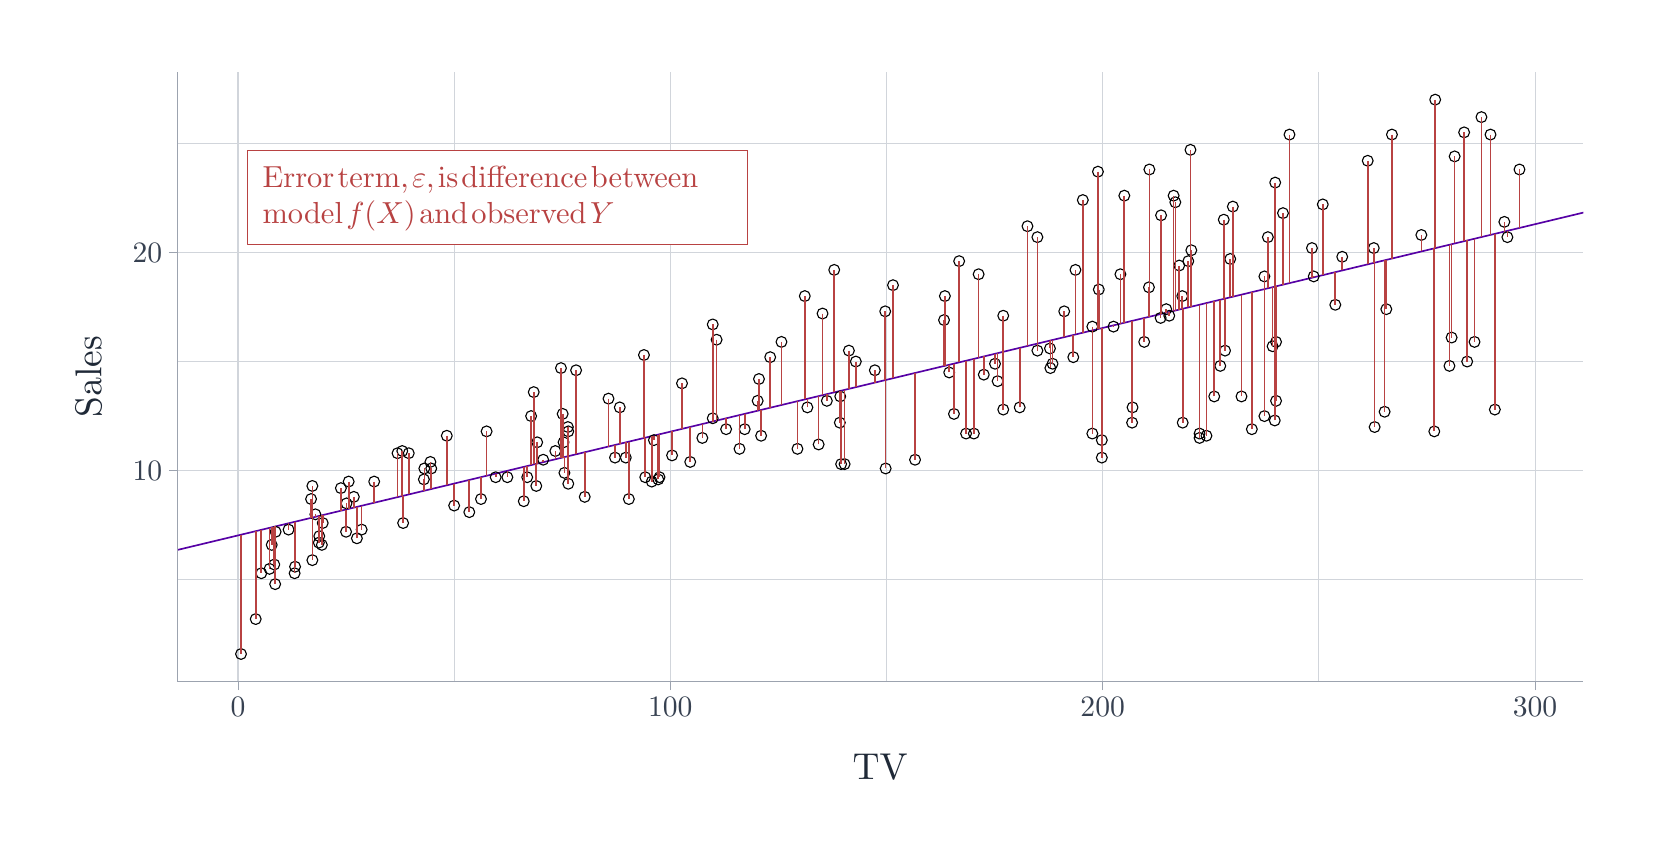
\begin{tikzpicture}[x=1pt,y=1pt]
\definecolor{fillColor}{RGB}{255,255,255}
\path[use as bounding box,fill=fillColor] (0,0) rectangle (578.16,289.08);
\begin{scope}
\path[clip] (  0.00,  0.00) rectangle (578.16,289.08);
\definecolor{drawColor}{RGB}{255,255,255}

\path[draw=drawColor,line width= 0.6pt,line join=round,line cap=round,fill=fillColor] (  0.00,  0.00) rectangle (578.16,289.08);
\end{scope}
\begin{scope}
\path[clip] ( 53.99, 52.74) rectangle (562.16,273.08);
\definecolor{drawColor}{RGB}{255,255,255}
\definecolor{fillColor}{RGB}{255,255,255}

\path[draw=drawColor,line width= 0.6pt,line join=round,line cap=round,fill=fillColor] ( 53.99, 52.74) rectangle (562.16,273.08);
\definecolor{drawColor}{RGB}{209,213,219}

\path[draw=drawColor,line width= 0.4pt,line join=round] ( 53.99, 89.57) --
	(562.16, 89.57);

\path[draw=drawColor,line width= 0.4pt,line join=round] ( 53.99,168.43) --
	(562.16,168.43);

\path[draw=drawColor,line width= 0.4pt,line join=round] ( 53.99,247.29) --
	(562.16,247.29);

\path[draw=drawColor,line width= 0.4pt,line join=round] (154.11, 52.74) --
	(154.11,273.08);

\path[draw=drawColor,line width= 0.4pt,line join=round] (310.34, 52.74) --
	(310.34,273.08);

\path[draw=drawColor,line width= 0.4pt,line join=round] (466.57, 52.74) --
	(466.57,273.08);

\path[draw=drawColor,line width= 0.4pt,line join=round] ( 53.99,129.00) --
	(562.16,129.00);

\path[draw=drawColor,line width= 0.4pt,line join=round] ( 53.99,207.86) --
	(562.16,207.86);

\path[draw=drawColor,line width= 0.4pt,line join=round] ( 75.99, 52.74) --
	( 75.99,273.08);

\path[draw=drawColor,line width= 0.4pt,line join=round] (232.22, 52.74) --
	(232.22,273.08);

\path[draw=drawColor,line width= 0.4pt,line join=round] (388.46, 52.74) --
	(388.46,273.08);

\path[draw=drawColor,line width= 0.4pt,line join=round] (544.69, 52.74) --
	(544.69,273.08);
\definecolor{drawColor}{RGB}{86,1,165}

\path[draw=drawColor,line width= 0.6pt,line join=round] (-454.18,-21.61) -- (1070.33,344.19);
\definecolor{drawColor}{RGB}{0,0,0}

\path[draw=drawColor,line width= 0.4pt,line join=round,line cap=round] (435.48,224.42) circle (  1.96);

\path[draw=drawColor,line width= 0.4pt,line join=round,line cap=round] (145.52,132.16) circle (  1.96);

\path[draw=drawColor,line width= 0.4pt,line join=round,line cap=round] (102.87,123.48) circle (  1.96);

\path[draw=drawColor,line width= 0.4pt,line join=round,line cap=round] (312.68,196.03) circle (  1.96);

\path[draw=drawColor,line width= 0.4pt,line join=round,line cap=round] (358.46,151.87) circle (  1.96);

\path[draw=drawColor,line width= 0.4pt,line join=round,line cap=round] ( 89.59,106.92) circle (  1.96);

\path[draw=drawColor,line width= 0.4pt,line join=round,line cap=round] (165.83,143.20) circle (  1.96);

\path[draw=drawColor,line width= 0.4pt,line join=round,line cap=round] (263.78,154.24) circle (  1.96);

\path[draw=drawColor,line width= 0.4pt,line join=round,line cap=round] ( 89.43, 88.00) circle (  1.96);

\path[draw=drawColor,line width= 0.4pt,line join=round,line cap=round] (388.14,133.73) circle (  1.96);

\path[draw=drawColor,line width= 0.4pt,line join=round,line cap=round] (179.26,117.96) circle (  1.96);

\path[draw=drawColor,line width= 0.4pt,line join=round,line cap=round] (411.42,187.36) circle (  1.96);

\path[draw=drawColor,line width= 0.4pt,line join=round,line cap=round] (113.18,122.69) circle (  1.96);

\path[draw=drawColor,line width= 0.4pt,line join=round,line cap=round] (228.32,126.64) circle (  1.96);

\path[draw=drawColor,line width= 0.4pt,line join=round,line cap=round] (394.86,199.98) circle (  1.96);

\path[draw=drawColor,line width= 0.4pt,line join=round,line cap=round] (381.27,226.79) circle (  1.96);

\path[draw=drawColor,line width= 0.4pt,line join=round,line cap=round] (181.92,148.72) circle (  1.96);

\path[draw=drawColor,line width= 0.4pt,line join=round,line cap=round] (515.63,242.56) circle (  1.96);

\path[draw=drawColor,line width= 0.4pt,line join=round,line cap=round] (184.11,139.25) circle (  1.96);

\path[draw=drawColor,line width= 0.4pt,line join=round,line cap=round] (306.12,165.28) circle (  1.96);

\path[draw=drawColor,line width= 0.4pt,line join=round,line cap=round] (417.20,192.09) circle (  1.96);

\path[draw=drawColor,line width= 0.4pt,line join=round,line cap=round] (446.89,148.72) circle (  1.96);

\path[draw=drawColor,line width= 0.4pt,line join=round,line cap=round] ( 96.62, 94.30) circle (  1.96);

\path[draw=drawColor,line width= 0.4pt,line join=round,line cap=round] (432.67,172.38) circle (  1.96);

\path[draw=drawColor,line width= 0.4pt,line join=round,line cap=round] (173.33,126.64) circle (  1.96);

\path[draw=drawColor,line width= 0.4pt,line join=round,line cap=round] (486.72,144.77) circle (  1.96);

\path[draw=drawColor,line width= 0.4pt,line join=round,line cap=round] (299.25,168.43) circle (  1.96);

\path[draw=drawColor,line width= 0.4pt,line join=round,line cap=round] (451.10,175.53) circle (  1.96);

\path[draw=drawColor,line width= 0.4pt,line join=round,line cap=round] (464.70,199.19) circle (  1.96);

\path[draw=drawColor,line width= 0.4pt,line join=round,line cap=round] (186.29,132.95) circle (  1.96);

\path[draw=drawColor,line width= 0.4pt,line join=round,line cap=round] (533.59,218.90) circle (  1.96);

\path[draw=drawColor,line width= 0.4pt,line join=round,line cap=round] (252.38,143.99) circle (  1.96);

\path[draw=drawColor,line width= 0.4pt,line join=round,line cap=round] (227.85,125.85) circle (  1.96);

\path[draw=drawColor,line width= 0.4pt,line join=round,line cap=round] (490.94,187.36) circle (  1.96);

\path[draw=drawColor,line width= 0.4pt,line join=round,line cap=round] (225.51,125.06) circle (  1.96);

\path[draw=drawColor,line width= 0.4pt,line join=round,line cap=round] (530.16,151.08) circle (  1.96);

\path[draw=drawColor,line width= 0.4pt,line join=round,line cap=round] (492.97,250.45) circle (  1.96);

\path[draw=drawColor,line width= 0.4pt,line join=round,line cap=round] (192.70,166.07) circle (  1.96);

\path[draw=drawColor,line width= 0.4pt,line join=round,line cap=round] (143.33,129.79) circle (  1.96);

\path[draw=drawColor,line width= 0.4pt,line join=round,line cap=round] (432.20,219.69) circle (  1.96);

\path[draw=drawColor,line width= 0.4pt,line join=round,line cap=round] (392.36,181.05) circle (  1.96);

\path[draw=drawColor,line width= 0.4pt,line join=round,line cap=round] (352.52,184.99) circle (  1.96);

\path[draw=drawColor,line width= 0.4pt,line join=round,line cap=round] (534.69,213.38) circle (  1.96);

\path[draw=drawColor,line width= 0.4pt,line join=round,line cap=round] (399.24,151.87) circle (  1.96);

\path[draw=drawColor,line width= 0.4pt,line join=round,line cap=round] (115.21,117.17) circle (  1.96);

\path[draw=drawColor,line width= 0.4pt,line join=round,line cap=round] (349.55,167.64) circle (  1.96);

\path[draw=drawColor,line width= 0.4pt,line join=round,line cap=round] (216.13,133.73) circle (  1.96);

\path[draw=drawColor,line width= 0.4pt,line join=round,line cap=round] (450.79,233.10) circle (  1.96);

\path[draw=drawColor,line width= 0.4pt,line join=round,line cap=round] (430.95,166.86) circle (  1.96);

\path[draw=drawColor,line width= 0.4pt,line join=round,line cap=round] (180.51,126.64) circle (  1.96);

\path[draw=drawColor,line width= 0.4pt,line join=round,line cap=round] (388.14,140.04) circle (  1.96);

\path[draw=drawColor,line width= 0.4pt,line join=round,line cap=round] (232.85,134.52) circle (  1.96);

\path[draw=drawColor,line width= 0.4pt,line join=round,line cap=round] (414.08,228.37) circle (  1.96);

\path[draw=drawColor,line width= 0.4pt,line join=round,line cap=round] (361.27,217.33) circle (  1.96);

\path[draw=drawColor,line width= 0.4pt,line join=round,line cap=round] (486.41,209.44) circle (  1.96);

\path[draw=drawColor,line width= 0.4pt,line join=round,line cap=round] (386.74,237.04) circle (  1.96);

\path[draw=drawColor,line width= 0.4pt,line join=round,line cap=round] ( 87.40, 93.52) circle (  1.96);

\path[draw=drawColor,line width= 0.4pt,line join=round,line cap=round] (288.78,154.24) circle (  1.96);

\path[draw=drawColor,line width= 0.4pt,line join=round,line cap=round] (405.33,237.83) circle (  1.96);

\path[draw=drawColor,line width= 0.4pt,line join=round,line cap=round] (405.17,195.25) circle (  1.96);

\path[draw=drawColor,line width= 0.4pt,line join=round,line cap=round] (159.58,114.02) circle (  1.96);

\path[draw=drawColor,line width= 0.4pt,line join=round,line cap=round] (484.22,240.98) circle (  1.96);

\path[draw=drawColor,line width= 0.4pt,line join=round,line cap=round] (449.85,173.95) circle (  1.96);

\path[draw=drawColor,line width= 0.4pt,line join=round,line cap=round] (236.44,160.55) circle (  1.96);

\path[draw=drawColor,line width= 0.4pt,line join=round,line cap=round] (280.81,192.09) circle (  1.96);

\path[draw=drawColor,line width= 0.4pt,line join=round,line cap=round] (183.79,123.48) circle (  1.96);

\path[draw=drawColor,line width= 0.4pt,line join=round,line cap=round] (125.21,125.06) circle (  1.96);

\path[draw=drawColor,line width= 0.4pt,line join=round,line cap=round] (293.62,155.82) circle (  1.96);

\path[draw=drawColor,line width= 0.4pt,line join=round,line cap=round] (446.89,199.19) circle (  1.96);

\path[draw=drawColor,line width= 0.4pt,line join=round,line cap=round] (414.70,226.00) circle (  1.96);

\path[draw=drawColor,line width= 0.4pt,line join=round,line cap=round] (387.05,194.46) circle (  1.96);

\path[draw=drawColor,line width= 0.4pt,line join=round,line cap=round] (247.54,147.93) circle (  1.96);

\path[draw=drawColor,line width= 0.4pt,line join=round,line cap=round] (117.86,119.54) circle (  1.96);

\path[draw=drawColor,line width= 0.4pt,line join=round,line cap=round] (278.16,136.89) circle (  1.96);

\path[draw=drawColor,line width= 0.4pt,line join=round,line cap=round] (409.39,184.20) circle (  1.96);

\path[draw=drawColor,line width= 0.4pt,line join=round,line cap=round] (102.40,118.75) circle (  1.96);

\path[draw=drawColor,line width= 0.4pt,line join=round,line cap=round] (118.96,104.56) circle (  1.96);

\path[draw=drawColor,line width= 0.4pt,line join=round,line cap=round] (264.25,162.12) circle (  1.96);

\path[draw=drawColor,line width= 0.4pt,line join=round,line cap=round] ( 84.43, 91.94) circle (  1.96);

\path[draw=drawColor,line width= 0.4pt,line join=round,line cap=round] (257.22,136.89) circle (  1.96);

\path[draw=drawColor,line width= 0.4pt,line join=round,line cap=round] (195.35,143.20) circle (  1.96);

\path[draw=drawColor,line width= 0.4pt,line join=round,line cap=round] (450.63,147.14) circle (  1.96);

\path[draw=drawColor,line width= 0.4pt,line join=round,line cap=round] (193.64,139.25) circle (  1.96);

\path[draw=drawColor,line width= 0.4pt,line join=round,line cap=round] (182.86,157.39) circle (  1.96);

\path[draw=drawColor,line width= 0.4pt,line join=round,line cap=round] (409.55,221.27) circle (  1.96);

\path[draw=drawColor,line width= 0.4pt,line join=round,line cap=round] (377.83,170.01) circle (  1.96);

\path[draw=drawColor,line width= 0.4pt,line join=round,line cap=round] (195.20,144.77) circle (  1.96);

\path[draw=drawColor,line width= 0.4pt,line join=round,line cap=round] (248.94,176.32) circle (  1.96);

\path[draw=drawColor,line width= 0.4pt,line join=round,line cap=round] (213.95,151.87) circle (  1.96);

\path[draw=drawColor,line width= 0.4pt,line join=round,line cap=round] (247.54,181.84) circle (  1.96);

\path[draw=drawColor,line width= 0.4pt,line join=round,line cap=round] (285.81,138.47) circle (  1.96);

\path[draw=drawColor,line width= 0.4pt,line join=round,line cap=round] (120.68,107.71) circle (  1.96);

\path[draw=drawColor,line width= 0.4pt,line join=round,line cap=round] (416.11,203.13) circle (  1.96);

\path[draw=drawColor,line width= 0.4pt,line join=round,line cap=round] (467.98,225.21) circle (  1.96);

\path[draw=drawColor,line width= 0.4pt,line join=round,line cap=round] (243.79,140.83) circle (  1.96);

\path[draw=drawColor,line width= 0.4pt,line join=round,line cap=round] (331.12,183.42) circle (  1.96);

\path[draw=drawColor,line width= 0.4pt,line join=round,line cap=round] (384.71,142.41) circle (  1.96);

\path[draw=drawColor,line width= 0.4pt,line join=round,line cap=round] (364.86,172.38) circle (  1.96);

\path[draw=drawColor,line width= 0.4pt,line join=round,line cap=round] (528.59,250.45) circle (  1.96);

\path[draw=drawColor,line width= 0.4pt,line join=round,line cap=round] (287.22,185.78) circle (  1.96);

\path[draw=drawColor,line width= 0.4pt,line join=round,line cap=round] (423.45,142.41) circle (  1.96);

\path[draw=drawColor,line width= 0.4pt,line join=round,line cap=round] (539.06,237.83) circle (  1.96);

\path[draw=drawColor,line width= 0.4pt,line join=round,line cap=round] (513.75,166.86) circle (  1.96);

\path[draw=drawColor,line width= 0.4pt,line join=round,line cap=round] (369.55,166.07) circle (  1.96);

\path[draw=drawColor,line width= 0.4pt,line join=round,line cap=round] (448.14,213.38) circle (  1.96);

\path[draw=drawColor,line width= 0.4pt,line join=round,line cap=round] (291.44,201.55) circle (  1.96);

\path[draw=drawColor,line width= 0.4pt,line join=round,line cap=round] (115.05,106.92) circle (  1.96);

\path[draw=drawColor,line width= 0.4pt,line join=round,line cap=round] (217.23,118.75) circle (  1.96);

\path[draw=drawColor,line width= 0.4pt,line join=round,line cap=round] ( 96.46, 91.94) circle (  1.96);

\path[draw=drawColor,line width= 0.4pt,line join=round,line cap=round] (475.01,206.29) circle (  1.96);

\path[draw=drawColor,line width= 0.4pt,line join=round,line cap=round] (428.76,155.82) circle (  1.96);

\path[draw=drawColor,line width= 0.4pt,line join=round,line cap=round] (453.60,222.06) circle (  1.96);

\path[draw=drawColor,line width= 0.4pt,line join=round,line cap=round] (350.49,161.34) circle (  1.96);

\path[draw=drawColor,line width= 0.4pt,line join=round,line cap=round] (403.45,175.53) circle (  1.96);

\path[draw=drawColor,line width= 0.4pt,line join=round,line cap=round] (198.17,165.28) circle (  1.96);

\path[draw=drawColor,line width= 0.4pt,line join=round,line cap=round] (193.32,149.51) circle (  1.96);

\path[draw=drawColor,line width= 0.4pt,line join=round,line cap=round] (293.47,146.35) circle (  1.96);

\path[draw=drawColor,line width= 0.4pt,line join=round,line cap=round] (195.35,124.27) circle (  1.96);

\path[draw=drawColor,line width= 0.4pt,line join=round,line cap=round] (272.38,175.53) circle (  1.96);

\path[draw=drawColor,line width= 0.4pt,line join=round,line cap=round] (106.30,102.19) circle (  1.96);

\path[draw=drawColor,line width= 0.4pt,line join=round,line cap=round] (296.75,172.38) circle (  1.96);

\path[draw=drawColor,line width= 0.4pt,line join=round,line cap=round] (105.37,105.34) circle (  1.96);

\path[draw=drawColor,line width= 0.4pt,line join=round,line cap=round] (425.95,141.62) circle (  1.96);

\path[draw=drawColor,line width= 0.4pt,line join=round,line cap=round] (268.31,170.01) circle (  1.96);

\path[draw=drawColor,line width= 0.4pt,line join=round,line cap=round] (434.54,205.50) circle (  1.96);

\path[draw=drawColor,line width= 0.4pt,line join=round,line cap=round] (212.23,133.73) circle (  1.96);

\path[draw=drawColor,line width= 0.4pt,line join=round,line cap=round] ( 88.18,102.19) circle (  1.96);

\path[draw=drawColor,line width= 0.4pt,line join=round,line cap=round] (201.29,119.54) circle (  1.96);

\path[draw=drawColor,line width= 0.4pt,line join=round,line cap=round] (420.17,244.93) circle (  1.96);

\path[draw=drawColor,line width= 0.4pt,line join=round,line cap=round] (169.11,126.64) circle (  1.96);

\path[draw=drawColor,line width= 0.4pt,line join=round,line cap=round] ( 77.09, 62.76) circle (  1.96);

\path[draw=drawColor,line width= 0.4pt,line join=round,line cap=round] (490.32,150.29) circle (  1.96);

\path[draw=drawColor,line width= 0.4pt,line join=round,line cap=round] ( 89.12, 95.09) circle (  1.96);

\path[draw=drawColor,line width= 0.4pt,line join=round,line cap=round] (419.39,204.71) circle (  1.96);

\path[draw=drawColor,line width= 0.4pt,line join=round,line cap=round] (133.64,135.31) circle (  1.96);

\path[draw=drawColor,line width= 0.4pt,line join=round,line cap=round] (151.45,141.62) circle (  1.96);

\path[draw=drawColor,line width= 0.4pt,line join=round,line cap=round] (115.99,125.06) circle (  1.96);

\path[draw=drawColor,line width= 0.4pt,line join=round,line cap=round] (503.60,214.17) circle (  1.96);

\path[draw=drawColor,line width= 0.4pt,line join=round,line cap=round] (143.17,125.85) circle (  1.96);

\path[draw=drawColor,line width= 0.4pt,line join=round,line cap=round] (364.86,213.38) circle (  1.96);

\path[draw=drawColor,line width= 0.4pt,line join=round,line cap=round] (190.67,136.10) circle (  1.96);

\path[draw=drawColor,line width= 0.4pt,line join=round,line cap=round] (378.61,201.55) circle (  1.96);

\path[draw=drawColor,line width= 0.4pt,line join=round,line cap=round] (420.48,208.65) circle (  1.96);

\path[draw=drawColor,line width= 0.4pt,line join=round,line cap=round] (239.41,132.16) circle (  1.96);

\path[draw=drawColor,line width= 0.4pt,line join=round,line cap=round] (226.29,140.04) circle (  1.96);

\path[draw=drawColor,line width= 0.4pt,line join=round,line cap=round] (295.19,131.37) circle (  1.96);

\path[draw=drawColor,line width= 0.4pt,line join=round,line cap=round] (451.10,154.24) circle (  1.96);

\path[draw=drawColor,line width= 0.4pt,line join=round,line cap=round] (455.95,250.45) circle (  1.96);

\path[draw=drawColor,line width= 0.4pt,line join=round,line cap=round] (135.36,136.10) circle (  1.96);

\path[draw=drawColor,line width= 0.4pt,line join=round,line cap=round] (145.83,129.79) circle (  1.96);

\path[draw=drawColor,line width= 0.4pt,line join=round,line cap=round] (514.53,177.11) circle (  1.96);

\path[draw=drawColor,line width= 0.4pt,line join=round,line cap=round] (265.03,141.62) circle (  1.96);

\path[draw=drawColor,line width= 0.4pt,line join=round,line cap=round] (384.71,181.05) circle (  1.96);

\path[draw=drawColor,line width= 0.4pt,line join=round,line cap=round] (343.62,199.98) circle (  1.96);

\path[draw=drawColor,line width= 0.4pt,line join=round,line cap=round] (369.40,173.16) circle (  1.96);

\path[draw=drawColor,line width= 0.4pt,line join=round,line cap=round] ( 82.40, 75.38) circle (  1.96);

\path[draw=drawColor,line width= 0.4pt,line join=round,line cap=round] (222.69,170.80) circle (  1.96);

\path[draw=drawColor,line width= 0.4pt,line join=round,line cap=round] (310.03,129.79) circle (  1.96);

\path[draw=drawColor,line width= 0.4pt,line join=round,line cap=round] ( 94.27,107.71) circle (  1.96);

\path[draw=drawColor,line width= 0.4pt,line join=round,line cap=round] (281.75,151.87) circle (  1.96);

\path[draw=drawColor,line width= 0.4pt,line join=round,line cap=round] (345.49,163.70) circle (  1.96);

\path[draw=drawColor,line width= 0.4pt,line join=round,line cap=round] (209.88,155.03) circle (  1.96);

\path[draw=drawColor,line width= 0.4pt,line join=round,line cap=round] (370.33,167.64) circle (  1.96);

\path[draw=drawColor,line width= 0.4pt,line join=round,line cap=round] (331.43,192.09) circle (  1.96);

\path[draw=drawColor,line width= 0.4pt,line join=round,line cap=round] (259.10,143.99) circle (  1.96);

\path[draw=drawColor,line width= 0.4pt,line join=round,line cap=round] (442.35,143.99) circle (  1.96);

\path[draw=drawColor,line width= 0.4pt,line join=round,line cap=round] (103.96,113.23) circle (  1.96);

\path[draw=drawColor,line width= 0.4pt,line join=round,line cap=round] (399.08,146.35) circle (  1.96);

\path[draw=drawColor,line width= 0.4pt,line join=round,line cap=round] (412.51,184.99) circle (  1.96);

\path[draw=drawColor,line width= 0.4pt,line join=round,line cap=round] (520.16,168.43) circle (  1.96);

\path[draw=drawColor,line width= 0.4pt,line join=round,line cap=round] (154.11,116.39) circle (  1.96);

\path[draw=drawColor,line width= 0.4pt,line join=round,line cap=round] (332.99,164.49) circle (  1.96);

\path[draw=drawColor,line width= 0.4pt,line join=round,line cap=round] (106.62,110.08) circle (  1.96);

\path[draw=drawColor,line width= 0.4pt,line join=round,line cap=round] (339.09,142.41) circle (  1.96);

\path[draw=drawColor,line width= 0.4pt,line join=round,line cap=round] (423.45,140.83) circle (  1.96);

\path[draw=drawColor,line width= 0.4pt,line join=round,line cap=round] (508.60,263.06) circle (  1.96);

\path[draw=drawColor,line width= 0.4pt,line join=round,line cap=round] (464.07,209.44) circle (  1.96);

\path[draw=drawColor,line width= 0.4pt,line join=round,line cap=round] (341.90,142.41) circle (  1.96);

\path[draw=drawColor,line width= 0.4pt,line join=round,line cap=round] (508.28,143.20) circle (  1.96);

\path[draw=drawColor,line width= 0.4pt,line join=round,line cap=round] (334.71,149.51) circle (  1.96);

\path[draw=drawColor,line width= 0.4pt,line join=round,line cap=round] (320.65,132.95) circle (  1.96);

\path[draw=drawColor,line width= 0.4pt,line join=round,line cap=round] (417.36,146.35) circle (  1.96);

\path[draw=drawColor,line width= 0.4pt,line join=round,line cap=round] (163.80,118.75) circle (  1.96);

\path[draw=drawColor,line width= 0.4pt,line join=round,line cap=round] (525.31,256.76) circle (  1.96);

\path[draw=drawColor,line width= 0.4pt,line join=round,line cap=round] (472.51,188.94) circle (  1.96);

\path[draw=drawColor,line width= 0.4pt,line join=round,line cap=round] (396.27,228.37) circle (  1.96);

\path[draw=drawColor,line width= 0.4pt,line join=round,line cap=round] (293.94,131.37) circle (  1.96);

\path[draw=drawColor,line width= 0.4pt,line join=round,line cap=round] (374.55,186.57) circle (  1.96);

\path[draw=drawColor,line width= 0.4pt,line join=round,line cap=round] (522.81,175.53) circle (  1.96);

\path[draw=drawColor,line width= 0.4pt,line join=round,line cap=round] (105.21,102.98) circle (  1.96);

\path[draw=drawColor,line width= 0.4pt,line join=round,line cap=round] (137.71,135.31) circle (  1.96);

\path[draw=drawColor,line width= 0.4pt,line join=round,line cap=round] (193.95,128.21) circle (  1.96);

\path[draw=drawColor,line width= 0.4pt,line join=round,line cap=round] (102.87, 96.67) circle (  1.96);

\path[draw=drawColor,line width= 0.4pt,line join=round,line cap=round] (336.59,204.71) circle (  1.96);

\path[draw=drawColor,line width= 0.4pt,line join=round,line cap=round] (309.87,186.57) circle (  1.96);

\path[draw=drawColor,line width= 0.4pt,line join=round,line cap=round] (135.67,110.08) circle (  1.96);

\path[draw=drawColor,line width= 0.4pt,line join=round,line cap=round] (223.16,126.64) circle (  1.96);

\path[draw=drawColor,line width= 0.4pt,line join=round,line cap=round] (352.52,151.08) circle (  1.96);

\path[draw=drawColor,line width= 0.4pt,line join=round,line cap=round] (519.06,251.24) circle (  1.96);

\path[draw=drawColor,line width= 0.4pt,line join=round,line cap=round] (438.61,155.82) circle (  1.96);
\definecolor{drawColor}{RGB}{184,66,66}

\path[draw=drawColor,line width= 0.6pt,line join=round] (435.48,224.42) -- (435.48,191.86);

\path[draw=drawColor,line width= 0.6pt,line join=round] (145.52,132.16) -- (145.52,122.28);

\path[draw=drawColor,line width= 0.6pt,line join=round] (102.87,123.48) -- (102.87,112.05);

\path[draw=drawColor,line width= 0.6pt,line join=round] (312.68,196.03) -- (312.68,162.40);

\path[draw=drawColor,line width= 0.6pt,line join=round] (358.46,151.87) -- (358.46,173.38);

\path[draw=drawColor,line width= 0.6pt,line join=round] ( 89.59,106.92) -- ( 89.59,108.86);

\path[draw=drawColor,line width= 0.6pt,line join=round] (165.83,143.20) -- (165.83,127.16);

\path[draw=drawColor,line width= 0.6pt,line join=round] (263.78,154.24) -- (263.78,150.66);

\path[draw=drawColor,line width= 0.6pt,line join=round] ( 89.43, 88.00) -- ( 89.43,108.83);

\path[draw=drawColor,line width= 0.6pt,line join=round] (388.14,133.73) -- (388.14,180.50);

\path[draw=drawColor,line width= 0.6pt,line join=round] (179.26,117.96) -- (179.26,130.38);

\path[draw=drawColor,line width= 0.6pt,line join=round] (411.42,187.36) -- (411.42,186.09);

\path[draw=drawColor,line width= 0.6pt,line join=round] (113.18,122.69) -- (113.18,114.52);

\path[draw=drawColor,line width= 0.6pt,line join=round] (228.32,126.64) -- (228.32,142.15);

\path[draw=drawColor,line width= 0.6pt,line join=round] (394.86,199.98) -- (394.86,182.11);

\path[draw=drawColor,line width= 0.6pt,line join=round] (381.27,226.79) -- (381.27,178.85);

\path[draw=drawColor,line width= 0.6pt,line join=round] (181.92,148.72) -- (181.92,131.02);

\path[draw=drawColor,line width= 0.6pt,line join=round] (515.63,242.56) -- (515.63,211.09);

\path[draw=drawColor,line width= 0.6pt,line join=round] (184.11,139.25) -- (184.11,131.54);

\path[draw=drawColor,line width= 0.6pt,line join=round] (306.12,165.28) -- (306.12,160.82);

\path[draw=drawColor,line width= 0.6pt,line join=round] (417.20,192.09) -- (417.20,187.47);

\path[draw=drawColor,line width= 0.6pt,line join=round] (446.89,148.72) -- (446.89,194.60);

\path[draw=drawColor,line width= 0.6pt,line join=round] ( 96.62, 94.30) -- ( 96.62,110.55);

\path[draw=drawColor,line width= 0.6pt,line join=round] (432.67,172.38) -- (432.67,191.19);

\path[draw=drawColor,line width= 0.6pt,line join=round] (173.33,126.64) -- (173.33,128.96);

\path[draw=drawColor,line width= 0.6pt,line join=round] (486.72,144.77) -- (486.72,204.16);

\path[draw=drawColor,line width= 0.6pt,line join=round] (299.25,168.43) -- (299.25,159.17);

\path[draw=drawColor,line width= 0.6pt,line join=round] (451.10,175.53) -- (451.10,195.61);

\path[draw=drawColor,line width= 0.6pt,line join=round] (464.70,199.19) -- (464.70,198.87);

\path[draw=drawColor,line width= 0.6pt,line join=round] (186.29,132.95) -- (186.29,132.07);

\path[draw=drawColor,line width= 0.6pt,line join=round] (533.59,218.90) -- (533.59,215.40);

\path[draw=drawColor,line width= 0.6pt,line join=round] (252.38,143.99) -- (252.38,147.92);

\path[draw=drawColor,line width= 0.6pt,line join=round] (227.85,125.85) -- (227.85,142.04);

\path[draw=drawColor,line width= 0.6pt,line join=round] (490.94,187.36) -- (490.94,205.17);

\path[draw=drawColor,line width= 0.6pt,line join=round] (225.51,125.06) -- (225.51,141.48);

\path[draw=drawColor,line width= 0.6pt,line join=round] (530.16,151.08) -- (530.16,214.58);

\path[draw=drawColor,line width= 0.6pt,line join=round] (492.97,250.45) -- (492.97,205.66);

\path[draw=drawColor,line width= 0.6pt,line join=round] (192.70,166.07) -- (192.70,133.60);

\path[draw=drawColor,line width= 0.6pt,line join=round] (143.33,129.79) -- (143.33,121.76);

\path[draw=drawColor,line width= 0.6pt,line join=round] (432.20,219.69) -- (432.20,191.07);

\path[draw=drawColor,line width= 0.6pt,line join=round] (392.36,181.05) -- (392.36,181.51);

\path[draw=drawColor,line width= 0.6pt,line join=round] (352.52,184.99) -- (352.52,171.95);

\path[draw=drawColor,line width= 0.6pt,line join=round] (534.69,213.38) -- (534.69,215.66);

\path[draw=drawColor,line width= 0.6pt,line join=round] (399.24,151.87) -- (399.24,183.16);

\path[draw=drawColor,line width= 0.6pt,line join=round] (115.21,117.17) -- (115.21,115.01);

\path[draw=drawColor,line width= 0.6pt,line join=round] (349.55,167.64) -- (349.55,171.24);

\path[draw=drawColor,line width= 0.6pt,line join=round] (216.13,133.73) -- (216.13,139.23);

\path[draw=drawColor,line width= 0.6pt,line join=round] (450.79,233.10) -- (450.79,195.53);

\path[draw=drawColor,line width= 0.6pt,line join=round] (430.95,166.86) -- (430.95,190.77);

\path[draw=drawColor,line width= 0.6pt,line join=round] (180.51,126.64) -- (180.51,130.68);

\path[draw=drawColor,line width= 0.6pt,line join=round] (388.14,140.04) -- (388.14,180.50);

\path[draw=drawColor,line width= 0.6pt,line join=round] (232.85,134.52) -- (232.85,143.24);

\path[draw=drawColor,line width= 0.6pt,line join=round] (414.08,228.37) -- (414.08,186.72);

\path[draw=drawColor,line width= 0.6pt,line join=round] (361.27,217.33) -- (361.27,174.05);

\path[draw=drawColor,line width= 0.6pt,line join=round] (486.41,209.44) -- (486.41,204.08);

\path[draw=drawColor,line width= 0.6pt,line join=round] (386.74,237.04) -- (386.74,180.16);

\path[draw=drawColor,line width= 0.6pt,line join=round] ( 87.40, 93.52) -- ( 87.40,108.34);

\path[draw=drawColor,line width= 0.6pt,line join=round] (288.78,154.24) -- (288.78,156.66);

\path[draw=drawColor,line width= 0.6pt,line join=round] (405.33,237.83) -- (405.33,184.63);

\path[draw=drawColor,line width= 0.6pt,line join=round] (405.17,195.25) -- (405.17,184.59);

\path[draw=drawColor,line width= 0.6pt,line join=round] (159.58,114.02) -- (159.58,125.66);

\path[draw=drawColor,line width= 0.6pt,line join=round] (484.22,240.98) -- (484.22,203.56);

\path[draw=drawColor,line width= 0.6pt,line join=round] (449.85,173.95) -- (449.85,195.31);

\path[draw=drawColor,line width= 0.6pt,line join=round] (236.44,160.55) -- (236.44,144.10);

\path[draw=drawColor,line width= 0.6pt,line join=round] (280.81,192.09) -- (280.81,154.75);

\path[draw=drawColor,line width= 0.6pt,line join=round] (183.79,123.48) -- (183.79,131.47);

\path[draw=drawColor,line width= 0.6pt,line join=round] (125.21,125.06) -- (125.21,117.41);

\path[draw=drawColor,line width= 0.6pt,line join=round] (293.62,155.82) -- (293.62,157.82);

\path[draw=drawColor,line width= 0.6pt,line join=round] (446.89,199.19) -- (446.89,194.60);

\path[draw=drawColor,line width= 0.6pt,line join=round] (414.70,226.00) -- (414.70,186.87);

\path[draw=drawColor,line width= 0.6pt,line join=round] (387.05,194.46) -- (387.05,180.24);

\path[draw=drawColor,line width= 0.6pt,line join=round] (247.54,147.93) -- (247.54,146.76);

\path[draw=drawColor,line width= 0.6pt,line join=round] (117.86,119.54) -- (117.86,115.65);

\path[draw=drawColor,line width= 0.6pt,line join=round] (278.16,136.89) -- (278.16,154.11);

\path[draw=drawColor,line width= 0.6pt,line join=round] (409.39,184.20) -- (409.39,185.60);

\path[draw=drawColor,line width= 0.6pt,line join=round] (102.40,118.75) -- (102.40,111.94);

\path[draw=drawColor,line width= 0.6pt,line join=round] (118.96,104.56) -- (118.96,115.91);

\path[draw=drawColor,line width= 0.6pt,line join=round] (264.25,162.12) -- (264.25,150.77);

\path[draw=drawColor,line width= 0.6pt,line join=round] ( 84.43, 91.94) -- ( 84.43,107.63);

\path[draw=drawColor,line width= 0.6pt,line join=round] (257.22,136.89) -- (257.22,149.09);

\path[draw=drawColor,line width= 0.6pt,line join=round] (195.35,143.20) -- (195.35,134.24);

\path[draw=drawColor,line width= 0.6pt,line join=round] (450.63,147.14) -- (450.63,195.50);

\path[draw=drawColor,line width= 0.6pt,line join=round] (193.64,139.25) -- (193.64,133.83);

\path[draw=drawColor,line width= 0.6pt,line join=round] (182.86,157.39) -- (182.86,131.24);

\path[draw=drawColor,line width= 0.6pt,line join=round] (409.55,221.27) -- (409.55,185.64);

\path[draw=drawColor,line width= 0.6pt,line join=round] (377.83,170.01) -- (377.83,178.03);

\path[draw=drawColor,line width= 0.6pt,line join=round] (195.20,144.77) -- (195.20,134.20);

\path[draw=drawColor,line width= 0.6pt,line join=round] (248.94,176.32) -- (248.94,147.10);

\path[draw=drawColor,line width= 0.6pt,line join=round] (213.95,151.87) -- (213.95,138.70);

\path[draw=drawColor,line width= 0.6pt,line join=round] (247.54,181.84) -- (247.54,146.76);

\path[draw=drawColor,line width= 0.6pt,line join=round] (285.81,138.47) -- (285.81,155.95);

\path[draw=drawColor,line width= 0.6pt,line join=round] (120.68,107.71) -- (120.68,116.32);

\path[draw=drawColor,line width= 0.6pt,line join=round] (416.11,203.13) -- (416.11,187.21);

\path[draw=drawColor,line width= 0.6pt,line join=round] (467.98,225.21) -- (467.98,199.66);

\path[draw=drawColor,line width= 0.6pt,line join=round] (243.79,140.83) -- (243.79,145.86);

\path[draw=drawColor,line width= 0.6pt,line join=round] (331.12,183.42) -- (331.12,166.82);

\path[draw=drawColor,line width= 0.6pt,line join=round] (384.71,142.41) -- (384.71,179.68);

\path[draw=drawColor,line width= 0.6pt,line join=round] (364.86,172.38) -- (364.86,174.92);

\path[draw=drawColor,line width= 0.6pt,line join=round] (528.59,250.45) -- (528.59,214.20);

\path[draw=drawColor,line width= 0.6pt,line join=round] (287.22,185.78) -- (287.22,156.28);

\path[draw=drawColor,line width= 0.6pt,line join=round] (423.45,142.41) -- (423.45,188.97);

\path[draw=drawColor,line width= 0.6pt,line join=round] (539.06,237.83) -- (539.06,216.71);

\path[draw=drawColor,line width= 0.6pt,line join=round] (513.75,166.86) -- (513.75,210.64);

\path[draw=drawColor,line width= 0.6pt,line join=round] (369.55,166.07) -- (369.55,176.04);

\path[draw=drawColor,line width= 0.6pt,line join=round] (448.14,213.38) -- (448.14,194.90);

\path[draw=drawColor,line width= 0.6pt,line join=round] (291.44,201.55) -- (291.44,157.30);

\path[draw=drawColor,line width= 0.6pt,line join=round] (115.05,106.92) -- (115.05,114.97);

\path[draw=drawColor,line width= 0.6pt,line join=round] (217.23,118.75) -- (217.23,139.49);

\path[draw=drawColor,line width= 0.6pt,line join=round] ( 96.46, 91.94) -- ( 96.46,110.51);

\path[draw=drawColor,line width= 0.6pt,line join=round] (475.01,206.29) -- (475.01,201.34);

\path[draw=drawColor,line width= 0.6pt,line join=round] (428.76,155.82) -- (428.76,190.25);

\path[draw=drawColor,line width= 0.6pt,line join=round] (453.60,222.06) -- (453.60,196.21);

\path[draw=drawColor,line width= 0.6pt,line join=round] (350.49,161.34) -- (350.49,171.47);

\path[draw=drawColor,line width= 0.6pt,line join=round] (403.45,175.53) -- (403.45,184.18);

\path[draw=drawColor,line width= 0.6pt,line join=round] (198.17,165.28) -- (198.17,134.92);

\path[draw=drawColor,line width= 0.6pt,line join=round] (193.32,149.51) -- (193.32,133.75);

\path[draw=drawColor,line width= 0.6pt,line join=round] (293.47,146.35) -- (293.47,157.78);

\path[draw=drawColor,line width= 0.6pt,line join=round] (195.35,124.27) -- (195.35,134.24);

\path[draw=drawColor,line width= 0.6pt,line join=round] (272.38,175.53) -- (272.38,152.72);

\path[draw=drawColor,line width= 0.6pt,line join=round] (106.30,102.19) -- (106.30,112.87);

\path[draw=drawColor,line width= 0.6pt,line join=round] (296.75,172.38) -- (296.75,158.57);

\path[draw=drawColor,line width= 0.6pt,line join=round] (105.37,105.34) -- (105.37,112.65);

\path[draw=drawColor,line width= 0.6pt,line join=round] (425.95,141.62) -- (425.95,189.57);

\path[draw=drawColor,line width= 0.6pt,line join=round] (268.31,170.01) -- (268.31,151.75);

\path[draw=drawColor,line width= 0.6pt,line join=round] (434.54,205.50) -- (434.54,191.64);

\path[draw=drawColor,line width= 0.6pt,line join=round] (212.23,133.73) -- (212.23,138.29);

\path[draw=drawColor,line width= 0.6pt,line join=round] ( 88.18,102.19) -- ( 88.18,108.53);

\path[draw=drawColor,line width= 0.6pt,line join=round] (201.29,119.54) -- (201.29,135.67);

\path[draw=drawColor,line width= 0.6pt,line join=round] (420.17,244.93) -- (420.17,188.19);

\path[draw=drawColor,line width= 0.6pt,line join=round] (169.11,126.64) -- (169.11,127.94);

\path[draw=drawColor,line width= 0.6pt,line join=round] ( 77.09, 62.76) -- ( 77.09,105.86);

\path[draw=drawColor,line width= 0.6pt,line join=round] (490.32,150.29) -- (490.32,205.02);

\path[draw=drawColor,line width= 0.6pt,line join=round] ( 89.12, 95.09) -- ( 89.12,108.75);

\path[draw=drawColor,line width= 0.6pt,line join=round] (419.39,204.71) -- (419.39,188.00);

\path[draw=drawColor,line width= 0.6pt,line join=round] (133.64,135.31) -- (133.64,119.43);

\path[draw=drawColor,line width= 0.6pt,line join=round] (151.45,141.62) -- (151.45,123.71);

\path[draw=drawColor,line width= 0.6pt,line join=round] (115.99,125.06) -- (115.99,115.20);

\path[draw=drawColor,line width= 0.6pt,line join=round] (503.60,214.17) -- (503.60,208.20);

\path[draw=drawColor,line width= 0.6pt,line join=round] (143.17,125.85) -- (143.17,121.72);

\path[draw=drawColor,line width= 0.6pt,line join=round] (364.86,213.38) -- (364.86,174.92);

\path[draw=drawColor,line width= 0.6pt,line join=round] (190.67,136.10) -- (190.67,133.12);

\path[draw=drawColor,line width= 0.6pt,line join=round] (378.61,201.55) -- (378.61,178.21);

\path[draw=drawColor,line width= 0.6pt,line join=round] (420.48,208.65) -- (420.48,188.26);

\path[draw=drawColor,line width= 0.6pt,line join=round] (239.41,132.16) -- (239.41,144.81);

\path[draw=drawColor,line width= 0.6pt,line join=round] (226.29,140.04) -- (226.29,141.66);

\path[draw=drawColor,line width= 0.6pt,line join=round] (295.19,131.37) -- (295.19,158.20);

\path[draw=drawColor,line width= 0.6pt,line join=round] (451.10,154.24) -- (451.10,195.61);

\path[draw=drawColor,line width= 0.6pt,line join=round] (455.95,250.45) -- (455.95,196.77);

\path[draw=drawColor,line width= 0.6pt,line join=round] (135.36,136.10) -- (135.36,119.85);

\path[draw=drawColor,line width= 0.6pt,line join=round] (145.83,129.79) -- (145.83,122.36);

\path[draw=drawColor,line width= 0.6pt,line join=round] (514.53,177.11) -- (514.53,210.83);

\path[draw=drawColor,line width= 0.6pt,line join=round] (265.03,141.62) -- (265.03,150.96);

\path[draw=drawColor,line width= 0.6pt,line join=round] (384.71,181.05) -- (384.71,179.68);

\path[draw=drawColor,line width= 0.6pt,line join=round] (343.62,199.98) -- (343.62,169.82);

\path[draw=drawColor,line width= 0.6pt,line join=round] (369.40,173.16) -- (369.40,176.00);

\path[draw=drawColor,line width= 0.6pt,line join=round] ( 82.40, 75.38) -- ( 82.40,107.14);

\path[draw=drawColor,line width= 0.6pt,line join=round] (222.69,170.80) -- (222.69,140.80);

\path[draw=drawColor,line width= 0.6pt,line join=round] (310.03,129.79) -- (310.03,161.76);

\path[draw=drawColor,line width= 0.6pt,line join=round] ( 94.27,107.71) -- ( 94.27,109.99);

\path[draw=drawColor,line width= 0.6pt,line join=round] (281.75,151.87) -- (281.75,154.97);

\path[draw=drawColor,line width= 0.6pt,line join=round] (345.49,163.70) -- (345.49,170.27);

\path[draw=drawColor,line width= 0.6pt,line join=round] (209.88,155.03) -- (209.88,137.73);

\path[draw=drawColor,line width= 0.6pt,line join=round] (370.33,167.64) -- (370.33,176.23);

\path[draw=drawColor,line width= 0.6pt,line join=round] (331.43,192.09) -- (331.43,166.89);

\path[draw=drawColor,line width= 0.6pt,line join=round] (259.10,143.99) -- (259.10,149.54);

\path[draw=drawColor,line width= 0.6pt,line join=round] (442.35,143.99) -- (442.35,193.51);

\path[draw=drawColor,line width= 0.6pt,line join=round] (103.96,113.23) -- (103.96,112.31);

\path[draw=drawColor,line width= 0.6pt,line join=round] (399.08,146.35) -- (399.08,183.13);

\path[draw=drawColor,line width= 0.6pt,line join=round] (412.51,184.99) -- (412.51,186.35);

\path[draw=drawColor,line width= 0.6pt,line join=round] (520.16,168.43) -- (520.16,212.18);

\path[draw=drawColor,line width= 0.6pt,line join=round] (154.11,116.39) -- (154.11,124.35);

\path[draw=drawColor,line width= 0.6pt,line join=round] (332.99,164.49) -- (332.99,167.27);

\path[draw=drawColor,line width= 0.6pt,line join=round] (106.62,110.08) -- (106.62,112.95);

\path[draw=drawColor,line width= 0.6pt,line join=round] (339.09,142.41) -- (339.09,168.73);

\path[draw=drawColor,line width= 0.6pt,line join=round] (423.45,140.83) -- (423.45,188.97);

\path[draw=drawColor,line width= 0.6pt,line join=round] (508.60,263.06) -- (508.60,209.40);

\path[draw=drawColor,line width= 0.6pt,line join=round] (464.07,209.44) -- (464.07,198.72);

\path[draw=drawColor,line width= 0.6pt,line join=round] (341.90,142.41) -- (341.90,169.41);

\path[draw=drawColor,line width= 0.6pt,line join=round] (508.28,143.20) -- (508.28,209.33);

\path[draw=drawColor,line width= 0.6pt,line join=round] (334.71,149.51) -- (334.71,167.68);

\path[draw=drawColor,line width= 0.6pt,line join=round] (320.65,132.95) -- (320.65,164.31);

\path[draw=drawColor,line width= 0.6pt,line join=round] (417.36,146.35) -- (417.36,187.51);

\path[draw=drawColor,line width= 0.6pt,line join=round] (163.80,118.75) -- (163.80,126.67);

\path[draw=drawColor,line width= 0.6pt,line join=round] (525.31,256.76) -- (525.31,213.42);

\path[draw=drawColor,line width= 0.6pt,line join=round] (472.51,188.94) -- (472.51,200.74);

\path[draw=drawColor,line width= 0.6pt,line join=round] (396.27,228.37) -- (396.27,182.45);

\path[draw=drawColor,line width= 0.6pt,line join=round] (293.94,131.37) -- (293.94,157.90);

\path[draw=drawColor,line width= 0.6pt,line join=round] (374.55,186.57) -- (374.55,177.24);

\path[draw=drawColor,line width= 0.6pt,line join=round] (522.81,175.53) -- (522.81,212.82);

\path[draw=drawColor,line width= 0.6pt,line join=round] (105.21,102.98) -- (105.21,112.61);

\path[draw=drawColor,line width= 0.6pt,line join=round] (137.71,135.31) -- (137.71,120.41);

\path[draw=drawColor,line width= 0.6pt,line join=round] (193.95,128.21) -- (193.95,133.90);

\path[draw=drawColor,line width= 0.6pt,line join=round] (102.87, 96.67) -- (102.87,112.05);

\path[draw=drawColor,line width= 0.6pt,line join=round] (336.59,204.71) -- (336.59,168.13);

\path[draw=drawColor,line width= 0.6pt,line join=round] (309.87,186.57) -- (309.87,161.72);

\path[draw=drawColor,line width= 0.6pt,line join=round] (135.67,110.08) -- (135.67,119.92);

\path[draw=drawColor,line width= 0.6pt,line join=round] (223.16,126.64) -- (223.16,140.91);

\path[draw=drawColor,line width= 0.6pt,line join=round] (352.52,151.08) -- (352.52,171.95);

\path[draw=drawColor,line width= 0.6pt,line join=round] (519.06,251.24) -- (519.06,211.92);

\path[draw=drawColor,line width= 0.6pt,line join=round] (438.61,155.82) -- (438.61,192.61);

\path[draw=drawColor,line width= 0.3pt,line join=round,line cap=round,fill=fillColor] ( 79.40,210.58) rectangle (260.07,244.58);

\node[text=drawColor,anchor=base west,inner sep=0pt, outer sep=0pt, scale=  1.10] at ( 84.90,231.47) {Error};

\node[text=drawColor,anchor=base west,inner sep=0pt, outer sep=0pt, scale=  1.10] at (112.00,231.47) {term,};

\node[text=drawColor,anchor=base west,inner sep=0pt, outer sep=0pt, scale=  1.10] at (138.89,231.47) {\(\varepsilon\),};

\node[text=drawColor,anchor=base west,inner sep=0pt, outer sep=0pt, scale=  1.10] at (148.20,231.47) {is};

\node[text=drawColor,anchor=base west,inner sep=0pt, outer sep=0pt, scale=  1.10] at (156.73,231.47) {difference};

\node[text=drawColor,anchor=base west,inner sep=0pt, outer sep=0pt, scale=  1.10] at (203.55,231.47) {between};

\node[text=drawColor,anchor=base west,inner sep=0pt, outer sep=0pt, scale=  1.10] at ( 84.90,218.23) {model};

\node[text=drawColor,anchor=base west,inner sep=0pt, outer sep=0pt, scale=  1.10] at (115.13,218.23) {\(f(X)\)};

\node[text=drawColor,anchor=base west,inner sep=0pt, outer sep=0pt, scale=  1.10] at (141.42,218.23) {and};

\node[text=drawColor,anchor=base west,inner sep=0pt, outer sep=0pt, scale=  1.10] at (160.31,218.23) {observed};

\node[text=drawColor,anchor=base west,inner sep=0pt, outer sep=0pt, scale=  1.10] at (203.20,218.23) {\(Y\)};
\end{scope}
\begin{scope}
\path[clip] ( 53.99, 52.74) rectangle (562.16,273.08);
\definecolor{drawColor}{RGB}{184,66,66}
\definecolor{fillColor}{RGB}{255,255,255}

\path[draw=drawColor,line width= 0.3pt,line join=round,line cap=round,fill=fillColor] ( 79.40,210.58) rectangle (260.07,244.58);

\node[text=drawColor,anchor=base west,inner sep=0pt, outer sep=0pt, scale=  1.10] at ( 84.90,231.47) {Error};

\node[text=drawColor,anchor=base west,inner sep=0pt, outer sep=0pt, scale=  1.10] at (112.00,231.47) {term,};

\node[text=drawColor,anchor=base west,inner sep=0pt, outer sep=0pt, scale=  1.10] at (138.89,231.47) {\(\varepsilon\),};

\node[text=drawColor,anchor=base west,inner sep=0pt, outer sep=0pt, scale=  1.10] at (148.20,231.47) {is};

\node[text=drawColor,anchor=base west,inner sep=0pt, outer sep=0pt, scale=  1.10] at (156.73,231.47) {difference};

\node[text=drawColor,anchor=base west,inner sep=0pt, outer sep=0pt, scale=  1.10] at (203.55,231.47) {between};

\node[text=drawColor,anchor=base west,inner sep=0pt, outer sep=0pt, scale=  1.10] at ( 84.90,218.23) {model};

\node[text=drawColor,anchor=base west,inner sep=0pt, outer sep=0pt, scale=  1.10] at (115.13,218.23) {\(f(X)\)};

\node[text=drawColor,anchor=base west,inner sep=0pt, outer sep=0pt, scale=  1.10] at (141.42,218.23) {and};

\node[text=drawColor,anchor=base west,inner sep=0pt, outer sep=0pt, scale=  1.10] at (160.31,218.23) {observed};

\node[text=drawColor,anchor=base west,inner sep=0pt, outer sep=0pt, scale=  1.10] at (203.20,218.23) {\(Y\)};
\end{scope}
\begin{scope}
\path[clip] ( 53.99, 52.74) rectangle (562.16,273.08);
\definecolor{drawColor}{RGB}{184,66,66}
\definecolor{fillColor}{RGB}{255,255,255}

\path[draw=drawColor,line width= 0.3pt,line join=round,line cap=round,fill=fillColor] ( 79.40,210.58) rectangle (260.07,244.58);

\node[text=drawColor,anchor=base west,inner sep=0pt, outer sep=0pt, scale=  1.10] at ( 84.90,231.47) {Error};

\node[text=drawColor,anchor=base west,inner sep=0pt, outer sep=0pt, scale=  1.10] at (112.00,231.47) {term,};

\node[text=drawColor,anchor=base west,inner sep=0pt, outer sep=0pt, scale=  1.10] at (138.89,231.47) {\(\varepsilon\),};

\node[text=drawColor,anchor=base west,inner sep=0pt, outer sep=0pt, scale=  1.10] at (148.20,231.47) {is};

\node[text=drawColor,anchor=base west,inner sep=0pt, outer sep=0pt, scale=  1.10] at (156.73,231.47) {difference};

\node[text=drawColor,anchor=base west,inner sep=0pt, outer sep=0pt, scale=  1.10] at (203.55,231.47) {between};

\node[text=drawColor,anchor=base west,inner sep=0pt, outer sep=0pt, scale=  1.10] at ( 84.90,218.23) {model};

\node[text=drawColor,anchor=base west,inner sep=0pt, outer sep=0pt, scale=  1.10] at (115.13,218.23) {\(f(X)\)};

\node[text=drawColor,anchor=base west,inner sep=0pt, outer sep=0pt, scale=  1.10] at (141.42,218.23) {and};

\node[text=drawColor,anchor=base west,inner sep=0pt, outer sep=0pt, scale=  1.10] at (160.31,218.23) {observed};

\node[text=drawColor,anchor=base west,inner sep=0pt, outer sep=0pt, scale=  1.10] at (203.20,218.23) {\(Y\)};
\end{scope}
\begin{scope}
\path[clip] ( 53.99, 52.74) rectangle (562.16,273.08);
\definecolor{drawColor}{RGB}{184,66,66}
\definecolor{fillColor}{RGB}{255,255,255}

\path[draw=drawColor,line width= 0.3pt,line join=round,line cap=round,fill=fillColor] ( 79.40,210.58) rectangle (260.07,244.58);

\node[text=drawColor,anchor=base west,inner sep=0pt, outer sep=0pt, scale=  1.10] at ( 84.90,231.47) {Error};

\node[text=drawColor,anchor=base west,inner sep=0pt, outer sep=0pt, scale=  1.10] at (112.00,231.47) {term,};

\node[text=drawColor,anchor=base west,inner sep=0pt, outer sep=0pt, scale=  1.10] at (138.89,231.47) {\(\varepsilon\),};

\node[text=drawColor,anchor=base west,inner sep=0pt, outer sep=0pt, scale=  1.10] at (148.20,231.47) {is};

\node[text=drawColor,anchor=base west,inner sep=0pt, outer sep=0pt, scale=  1.10] at (156.73,231.47) {difference};

\node[text=drawColor,anchor=base west,inner sep=0pt, outer sep=0pt, scale=  1.10] at (203.55,231.47) {between};

\node[text=drawColor,anchor=base west,inner sep=0pt, outer sep=0pt, scale=  1.10] at ( 84.90,218.23) {model};

\node[text=drawColor,anchor=base west,inner sep=0pt, outer sep=0pt, scale=  1.10] at (115.13,218.23) {\(f(X)\)};

\node[text=drawColor,anchor=base west,inner sep=0pt, outer sep=0pt, scale=  1.10] at (141.42,218.23) {and};

\node[text=drawColor,anchor=base west,inner sep=0pt, outer sep=0pt, scale=  1.10] at (160.31,218.23) {observed};

\node[text=drawColor,anchor=base west,inner sep=0pt, outer sep=0pt, scale=  1.10] at (203.20,218.23) {\(Y\)};
\end{scope}
\begin{scope}
\path[clip] ( 53.99, 52.74) rectangle (562.16,273.08);
\definecolor{drawColor}{RGB}{184,66,66}
\definecolor{fillColor}{RGB}{255,255,255}

\path[draw=drawColor,line width= 0.3pt,line join=round,line cap=round,fill=fillColor] ( 79.40,210.58) rectangle (260.07,244.58);

\node[text=drawColor,anchor=base west,inner sep=0pt, outer sep=0pt, scale=  1.10] at ( 84.90,231.47) {Error};

\node[text=drawColor,anchor=base west,inner sep=0pt, outer sep=0pt, scale=  1.10] at (112.00,231.47) {term,};

\node[text=drawColor,anchor=base west,inner sep=0pt, outer sep=0pt, scale=  1.10] at (138.89,231.47) {\(\varepsilon\),};

\node[text=drawColor,anchor=base west,inner sep=0pt, outer sep=0pt, scale=  1.10] at (148.20,231.47) {is};

\node[text=drawColor,anchor=base west,inner sep=0pt, outer sep=0pt, scale=  1.10] at (156.73,231.47) {difference};

\node[text=drawColor,anchor=base west,inner sep=0pt, outer sep=0pt, scale=  1.10] at (203.55,231.47) {between};

\node[text=drawColor,anchor=base west,inner sep=0pt, outer sep=0pt, scale=  1.10] at ( 84.90,218.23) {model};

\node[text=drawColor,anchor=base west,inner sep=0pt, outer sep=0pt, scale=  1.10] at (115.13,218.23) {\(f(X)\)};

\node[text=drawColor,anchor=base west,inner sep=0pt, outer sep=0pt, scale=  1.10] at (141.42,218.23) {and};

\node[text=drawColor,anchor=base west,inner sep=0pt, outer sep=0pt, scale=  1.10] at (160.31,218.23) {observed};

\node[text=drawColor,anchor=base west,inner sep=0pt, outer sep=0pt, scale=  1.10] at (203.20,218.23) {\(Y\)};
\end{scope}
\begin{scope}
\path[clip] ( 53.99, 52.74) rectangle (562.16,273.08);
\definecolor{drawColor}{RGB}{184,66,66}
\definecolor{fillColor}{RGB}{255,255,255}

\path[draw=drawColor,line width= 0.3pt,line join=round,line cap=round,fill=fillColor] ( 79.40,210.58) rectangle (260.07,244.58);

\node[text=drawColor,anchor=base west,inner sep=0pt, outer sep=0pt, scale=  1.10] at ( 84.90,231.47) {Error};

\node[text=drawColor,anchor=base west,inner sep=0pt, outer sep=0pt, scale=  1.10] at (112.00,231.47) {term,};

\node[text=drawColor,anchor=base west,inner sep=0pt, outer sep=0pt, scale=  1.10] at (138.89,231.47) {\(\varepsilon\),};

\node[text=drawColor,anchor=base west,inner sep=0pt, outer sep=0pt, scale=  1.10] at (148.20,231.47) {is};

\node[text=drawColor,anchor=base west,inner sep=0pt, outer sep=0pt, scale=  1.10] at (156.73,231.47) {difference};

\node[text=drawColor,anchor=base west,inner sep=0pt, outer sep=0pt, scale=  1.10] at (203.55,231.47) {between};

\node[text=drawColor,anchor=base west,inner sep=0pt, outer sep=0pt, scale=  1.10] at ( 84.90,218.23) {model};

\node[text=drawColor,anchor=base west,inner sep=0pt, outer sep=0pt, scale=  1.10] at (115.13,218.23) {\(f(X)\)};

\node[text=drawColor,anchor=base west,inner sep=0pt, outer sep=0pt, scale=  1.10] at (141.42,218.23) {and};

\node[text=drawColor,anchor=base west,inner sep=0pt, outer sep=0pt, scale=  1.10] at (160.31,218.23) {observed};

\node[text=drawColor,anchor=base west,inner sep=0pt, outer sep=0pt, scale=  1.10] at (203.20,218.23) {\(Y\)};
\end{scope}
\begin{scope}
\path[clip] ( 53.99, 52.74) rectangle (562.16,273.08);
\definecolor{drawColor}{RGB}{184,66,66}
\definecolor{fillColor}{RGB}{255,255,255}

\path[draw=drawColor,line width= 0.3pt,line join=round,line cap=round,fill=fillColor] ( 79.40,210.58) rectangle (260.07,244.58);

\node[text=drawColor,anchor=base west,inner sep=0pt, outer sep=0pt, scale=  1.10] at ( 84.90,231.47) {Error};

\node[text=drawColor,anchor=base west,inner sep=0pt, outer sep=0pt, scale=  1.10] at (112.00,231.47) {term,};

\node[text=drawColor,anchor=base west,inner sep=0pt, outer sep=0pt, scale=  1.10] at (138.89,231.47) {\(\varepsilon\),};

\node[text=drawColor,anchor=base west,inner sep=0pt, outer sep=0pt, scale=  1.10] at (148.20,231.47) {is};

\node[text=drawColor,anchor=base west,inner sep=0pt, outer sep=0pt, scale=  1.10] at (156.73,231.47) {difference};

\node[text=drawColor,anchor=base west,inner sep=0pt, outer sep=0pt, scale=  1.10] at (203.55,231.47) {between};

\node[text=drawColor,anchor=base west,inner sep=0pt, outer sep=0pt, scale=  1.10] at ( 84.90,218.23) {model};

\node[text=drawColor,anchor=base west,inner sep=0pt, outer sep=0pt, scale=  1.10] at (115.13,218.23) {\(f(X)\)};

\node[text=drawColor,anchor=base west,inner sep=0pt, outer sep=0pt, scale=  1.10] at (141.42,218.23) {and};

\node[text=drawColor,anchor=base west,inner sep=0pt, outer sep=0pt, scale=  1.10] at (160.31,218.23) {observed};

\node[text=drawColor,anchor=base west,inner sep=0pt, outer sep=0pt, scale=  1.10] at (203.20,218.23) {\(Y\)};
\end{scope}
\begin{scope}
\path[clip] ( 53.99, 52.74) rectangle (562.16,273.08);
\definecolor{drawColor}{RGB}{184,66,66}
\definecolor{fillColor}{RGB}{255,255,255}

\path[draw=drawColor,line width= 0.3pt,line join=round,line cap=round,fill=fillColor] ( 79.40,210.58) rectangle (260.07,244.58);

\node[text=drawColor,anchor=base west,inner sep=0pt, outer sep=0pt, scale=  1.10] at ( 84.90,231.47) {Error};

\node[text=drawColor,anchor=base west,inner sep=0pt, outer sep=0pt, scale=  1.10] at (112.00,231.47) {term,};

\node[text=drawColor,anchor=base west,inner sep=0pt, outer sep=0pt, scale=  1.10] at (138.89,231.47) {\(\varepsilon\),};

\node[text=drawColor,anchor=base west,inner sep=0pt, outer sep=0pt, scale=  1.10] at (148.20,231.47) {is};

\node[text=drawColor,anchor=base west,inner sep=0pt, outer sep=0pt, scale=  1.10] at (156.73,231.47) {difference};

\node[text=drawColor,anchor=base west,inner sep=0pt, outer sep=0pt, scale=  1.10] at (203.55,231.47) {between};

\node[text=drawColor,anchor=base west,inner sep=0pt, outer sep=0pt, scale=  1.10] at ( 84.90,218.23) {model};

\node[text=drawColor,anchor=base west,inner sep=0pt, outer sep=0pt, scale=  1.10] at (115.13,218.23) {\(f(X)\)};

\node[text=drawColor,anchor=base west,inner sep=0pt, outer sep=0pt, scale=  1.10] at (141.42,218.23) {and};

\node[text=drawColor,anchor=base west,inner sep=0pt, outer sep=0pt, scale=  1.10] at (160.31,218.23) {observed};

\node[text=drawColor,anchor=base west,inner sep=0pt, outer sep=0pt, scale=  1.10] at (203.20,218.23) {\(Y\)};
\end{scope}
\begin{scope}
\path[clip] ( 53.99, 52.74) rectangle (562.16,273.08);
\definecolor{drawColor}{RGB}{184,66,66}
\definecolor{fillColor}{RGB}{255,255,255}

\path[draw=drawColor,line width= 0.3pt,line join=round,line cap=round,fill=fillColor] ( 79.40,210.58) rectangle (260.07,244.58);

\node[text=drawColor,anchor=base west,inner sep=0pt, outer sep=0pt, scale=  1.10] at ( 84.90,231.47) {Error};

\node[text=drawColor,anchor=base west,inner sep=0pt, outer sep=0pt, scale=  1.10] at (112.00,231.47) {term,};

\node[text=drawColor,anchor=base west,inner sep=0pt, outer sep=0pt, scale=  1.10] at (138.89,231.47) {\(\varepsilon\),};

\node[text=drawColor,anchor=base west,inner sep=0pt, outer sep=0pt, scale=  1.10] at (148.20,231.47) {is};

\node[text=drawColor,anchor=base west,inner sep=0pt, outer sep=0pt, scale=  1.10] at (156.73,231.47) {difference};

\node[text=drawColor,anchor=base west,inner sep=0pt, outer sep=0pt, scale=  1.10] at (203.55,231.47) {between};

\node[text=drawColor,anchor=base west,inner sep=0pt, outer sep=0pt, scale=  1.10] at ( 84.90,218.23) {model};

\node[text=drawColor,anchor=base west,inner sep=0pt, outer sep=0pt, scale=  1.10] at (115.13,218.23) {\(f(X)\)};

\node[text=drawColor,anchor=base west,inner sep=0pt, outer sep=0pt, scale=  1.10] at (141.42,218.23) {and};

\node[text=drawColor,anchor=base west,inner sep=0pt, outer sep=0pt, scale=  1.10] at (160.31,218.23) {observed};

\node[text=drawColor,anchor=base west,inner sep=0pt, outer sep=0pt, scale=  1.10] at (203.20,218.23) {\(Y\)};
\end{scope}
\begin{scope}
\path[clip] ( 53.99, 52.74) rectangle (562.16,273.08);
\definecolor{drawColor}{RGB}{184,66,66}
\definecolor{fillColor}{RGB}{255,255,255}

\path[draw=drawColor,line width= 0.3pt,line join=round,line cap=round,fill=fillColor] ( 79.40,210.58) rectangle (260.07,244.58);

\node[text=drawColor,anchor=base west,inner sep=0pt, outer sep=0pt, scale=  1.10] at ( 84.90,231.47) {Error};

\node[text=drawColor,anchor=base west,inner sep=0pt, outer sep=0pt, scale=  1.10] at (112.00,231.47) {term,};

\node[text=drawColor,anchor=base west,inner sep=0pt, outer sep=0pt, scale=  1.10] at (138.89,231.47) {\(\varepsilon\),};

\node[text=drawColor,anchor=base west,inner sep=0pt, outer sep=0pt, scale=  1.10] at (148.20,231.47) {is};

\node[text=drawColor,anchor=base west,inner sep=0pt, outer sep=0pt, scale=  1.10] at (156.73,231.47) {difference};

\node[text=drawColor,anchor=base west,inner sep=0pt, outer sep=0pt, scale=  1.10] at (203.55,231.47) {between};

\node[text=drawColor,anchor=base west,inner sep=0pt, outer sep=0pt, scale=  1.10] at ( 84.90,218.23) {model};

\node[text=drawColor,anchor=base west,inner sep=0pt, outer sep=0pt, scale=  1.10] at (115.13,218.23) {\(f(X)\)};

\node[text=drawColor,anchor=base west,inner sep=0pt, outer sep=0pt, scale=  1.10] at (141.42,218.23) {and};

\node[text=drawColor,anchor=base west,inner sep=0pt, outer sep=0pt, scale=  1.10] at (160.31,218.23) {observed};

\node[text=drawColor,anchor=base west,inner sep=0pt, outer sep=0pt, scale=  1.10] at (203.20,218.23) {\(Y\)};
\end{scope}
\begin{scope}
\path[clip] ( 53.99, 52.74) rectangle (562.16,273.08);
\definecolor{drawColor}{RGB}{184,66,66}
\definecolor{fillColor}{RGB}{255,255,255}

\path[draw=drawColor,line width= 0.3pt,line join=round,line cap=round,fill=fillColor] ( 79.40,210.58) rectangle (260.07,244.58);

\node[text=drawColor,anchor=base west,inner sep=0pt, outer sep=0pt, scale=  1.10] at ( 84.90,231.47) {Error};

\node[text=drawColor,anchor=base west,inner sep=0pt, outer sep=0pt, scale=  1.10] at (112.00,231.47) {term,};

\node[text=drawColor,anchor=base west,inner sep=0pt, outer sep=0pt, scale=  1.10] at (138.89,231.47) {\(\varepsilon\),};

\node[text=drawColor,anchor=base west,inner sep=0pt, outer sep=0pt, scale=  1.10] at (148.20,231.47) {is};

\node[text=drawColor,anchor=base west,inner sep=0pt, outer sep=0pt, scale=  1.10] at (156.73,231.47) {difference};

\node[text=drawColor,anchor=base west,inner sep=0pt, outer sep=0pt, scale=  1.10] at (203.55,231.47) {between};

\node[text=drawColor,anchor=base west,inner sep=0pt, outer sep=0pt, scale=  1.10] at ( 84.90,218.23) {model};

\node[text=drawColor,anchor=base west,inner sep=0pt, outer sep=0pt, scale=  1.10] at (115.13,218.23) {\(f(X)\)};

\node[text=drawColor,anchor=base west,inner sep=0pt, outer sep=0pt, scale=  1.10] at (141.42,218.23) {and};

\node[text=drawColor,anchor=base west,inner sep=0pt, outer sep=0pt, scale=  1.10] at (160.31,218.23) {observed};

\node[text=drawColor,anchor=base west,inner sep=0pt, outer sep=0pt, scale=  1.10] at (203.20,218.23) {\(Y\)};
\end{scope}
\begin{scope}
\path[clip] ( 53.99, 52.74) rectangle (562.16,273.08);
\definecolor{drawColor}{RGB}{184,66,66}
\definecolor{fillColor}{RGB}{255,255,255}

\path[draw=drawColor,line width= 0.3pt,line join=round,line cap=round,fill=fillColor] ( 79.40,210.58) rectangle (260.07,244.58);

\node[text=drawColor,anchor=base west,inner sep=0pt, outer sep=0pt, scale=  1.10] at ( 84.90,231.47) {Error};

\node[text=drawColor,anchor=base west,inner sep=0pt, outer sep=0pt, scale=  1.10] at (112.00,231.47) {term,};

\node[text=drawColor,anchor=base west,inner sep=0pt, outer sep=0pt, scale=  1.10] at (138.89,231.47) {\(\varepsilon\),};

\node[text=drawColor,anchor=base west,inner sep=0pt, outer sep=0pt, scale=  1.10] at (148.20,231.47) {is};

\node[text=drawColor,anchor=base west,inner sep=0pt, outer sep=0pt, scale=  1.10] at (156.73,231.47) {difference};

\node[text=drawColor,anchor=base west,inner sep=0pt, outer sep=0pt, scale=  1.10] at (203.55,231.47) {between};

\node[text=drawColor,anchor=base west,inner sep=0pt, outer sep=0pt, scale=  1.10] at ( 84.90,218.23) {model};

\node[text=drawColor,anchor=base west,inner sep=0pt, outer sep=0pt, scale=  1.10] at (115.13,218.23) {\(f(X)\)};

\node[text=drawColor,anchor=base west,inner sep=0pt, outer sep=0pt, scale=  1.10] at (141.42,218.23) {and};

\node[text=drawColor,anchor=base west,inner sep=0pt, outer sep=0pt, scale=  1.10] at (160.31,218.23) {observed};

\node[text=drawColor,anchor=base west,inner sep=0pt, outer sep=0pt, scale=  1.10] at (203.20,218.23) {\(Y\)};
\end{scope}
\begin{scope}
\path[clip] ( 53.99, 52.74) rectangle (562.16,273.08);
\definecolor{drawColor}{RGB}{184,66,66}
\definecolor{fillColor}{RGB}{255,255,255}

\path[draw=drawColor,line width= 0.3pt,line join=round,line cap=round,fill=fillColor] ( 79.40,210.58) rectangle (260.07,244.58);

\node[text=drawColor,anchor=base west,inner sep=0pt, outer sep=0pt, scale=  1.10] at ( 84.90,231.47) {Error};

\node[text=drawColor,anchor=base west,inner sep=0pt, outer sep=0pt, scale=  1.10] at (112.00,231.47) {term,};

\node[text=drawColor,anchor=base west,inner sep=0pt, outer sep=0pt, scale=  1.10] at (138.89,231.47) {\(\varepsilon\),};

\node[text=drawColor,anchor=base west,inner sep=0pt, outer sep=0pt, scale=  1.10] at (148.20,231.47) {is};

\node[text=drawColor,anchor=base west,inner sep=0pt, outer sep=0pt, scale=  1.10] at (156.73,231.47) {difference};

\node[text=drawColor,anchor=base west,inner sep=0pt, outer sep=0pt, scale=  1.10] at (203.55,231.47) {between};

\node[text=drawColor,anchor=base west,inner sep=0pt, outer sep=0pt, scale=  1.10] at ( 84.90,218.23) {model};

\node[text=drawColor,anchor=base west,inner sep=0pt, outer sep=0pt, scale=  1.10] at (115.13,218.23) {\(f(X)\)};

\node[text=drawColor,anchor=base west,inner sep=0pt, outer sep=0pt, scale=  1.10] at (141.42,218.23) {and};

\node[text=drawColor,anchor=base west,inner sep=0pt, outer sep=0pt, scale=  1.10] at (160.31,218.23) {observed};

\node[text=drawColor,anchor=base west,inner sep=0pt, outer sep=0pt, scale=  1.10] at (203.20,218.23) {\(Y\)};
\end{scope}
\begin{scope}
\path[clip] ( 53.99, 52.74) rectangle (562.16,273.08);
\definecolor{drawColor}{RGB}{184,66,66}
\definecolor{fillColor}{RGB}{255,255,255}

\path[draw=drawColor,line width= 0.3pt,line join=round,line cap=round,fill=fillColor] ( 79.40,210.58) rectangle (260.07,244.58);

\node[text=drawColor,anchor=base west,inner sep=0pt, outer sep=0pt, scale=  1.10] at ( 84.90,231.47) {Error};

\node[text=drawColor,anchor=base west,inner sep=0pt, outer sep=0pt, scale=  1.10] at (112.00,231.47) {term,};

\node[text=drawColor,anchor=base west,inner sep=0pt, outer sep=0pt, scale=  1.10] at (138.89,231.47) {\(\varepsilon\),};

\node[text=drawColor,anchor=base west,inner sep=0pt, outer sep=0pt, scale=  1.10] at (148.20,231.47) {is};

\node[text=drawColor,anchor=base west,inner sep=0pt, outer sep=0pt, scale=  1.10] at (156.73,231.47) {difference};

\node[text=drawColor,anchor=base west,inner sep=0pt, outer sep=0pt, scale=  1.10] at (203.55,231.47) {between};

\node[text=drawColor,anchor=base west,inner sep=0pt, outer sep=0pt, scale=  1.10] at ( 84.90,218.23) {model};

\node[text=drawColor,anchor=base west,inner sep=0pt, outer sep=0pt, scale=  1.10] at (115.13,218.23) {\(f(X)\)};

\node[text=drawColor,anchor=base west,inner sep=0pt, outer sep=0pt, scale=  1.10] at (141.42,218.23) {and};

\node[text=drawColor,anchor=base west,inner sep=0pt, outer sep=0pt, scale=  1.10] at (160.31,218.23) {observed};

\node[text=drawColor,anchor=base west,inner sep=0pt, outer sep=0pt, scale=  1.10] at (203.20,218.23) {\(Y\)};
\end{scope}
\begin{scope}
\path[clip] ( 53.99, 52.74) rectangle (562.16,273.08);
\definecolor{drawColor}{RGB}{184,66,66}
\definecolor{fillColor}{RGB}{255,255,255}

\path[draw=drawColor,line width= 0.3pt,line join=round,line cap=round,fill=fillColor] ( 79.40,210.58) rectangle (260.07,244.58);

\node[text=drawColor,anchor=base west,inner sep=0pt, outer sep=0pt, scale=  1.10] at ( 84.90,231.47) {Error};

\node[text=drawColor,anchor=base west,inner sep=0pt, outer sep=0pt, scale=  1.10] at (112.00,231.47) {term,};

\node[text=drawColor,anchor=base west,inner sep=0pt, outer sep=0pt, scale=  1.10] at (138.89,231.47) {\(\varepsilon\),};

\node[text=drawColor,anchor=base west,inner sep=0pt, outer sep=0pt, scale=  1.10] at (148.20,231.47) {is};

\node[text=drawColor,anchor=base west,inner sep=0pt, outer sep=0pt, scale=  1.10] at (156.73,231.47) {difference};

\node[text=drawColor,anchor=base west,inner sep=0pt, outer sep=0pt, scale=  1.10] at (203.55,231.47) {between};

\node[text=drawColor,anchor=base west,inner sep=0pt, outer sep=0pt, scale=  1.10] at ( 84.90,218.23) {model};

\node[text=drawColor,anchor=base west,inner sep=0pt, outer sep=0pt, scale=  1.10] at (115.13,218.23) {\(f(X)\)};

\node[text=drawColor,anchor=base west,inner sep=0pt, outer sep=0pt, scale=  1.10] at (141.42,218.23) {and};

\node[text=drawColor,anchor=base west,inner sep=0pt, outer sep=0pt, scale=  1.10] at (160.31,218.23) {observed};

\node[text=drawColor,anchor=base west,inner sep=0pt, outer sep=0pt, scale=  1.10] at (203.20,218.23) {\(Y\)};
\end{scope}
\begin{scope}
\path[clip] ( 53.99, 52.74) rectangle (562.16,273.08);
\definecolor{drawColor}{RGB}{184,66,66}
\definecolor{fillColor}{RGB}{255,255,255}

\path[draw=drawColor,line width= 0.3pt,line join=round,line cap=round,fill=fillColor] ( 79.40,210.58) rectangle (260.07,244.58);

\node[text=drawColor,anchor=base west,inner sep=0pt, outer sep=0pt, scale=  1.10] at ( 84.90,231.47) {Error};

\node[text=drawColor,anchor=base west,inner sep=0pt, outer sep=0pt, scale=  1.10] at (112.00,231.47) {term,};

\node[text=drawColor,anchor=base west,inner sep=0pt, outer sep=0pt, scale=  1.10] at (138.89,231.47) {\(\varepsilon\),};

\node[text=drawColor,anchor=base west,inner sep=0pt, outer sep=0pt, scale=  1.10] at (148.20,231.47) {is};

\node[text=drawColor,anchor=base west,inner sep=0pt, outer sep=0pt, scale=  1.10] at (156.73,231.47) {difference};

\node[text=drawColor,anchor=base west,inner sep=0pt, outer sep=0pt, scale=  1.10] at (203.55,231.47) {between};

\node[text=drawColor,anchor=base west,inner sep=0pt, outer sep=0pt, scale=  1.10] at ( 84.90,218.23) {model};

\node[text=drawColor,anchor=base west,inner sep=0pt, outer sep=0pt, scale=  1.10] at (115.13,218.23) {\(f(X)\)};

\node[text=drawColor,anchor=base west,inner sep=0pt, outer sep=0pt, scale=  1.10] at (141.42,218.23) {and};

\node[text=drawColor,anchor=base west,inner sep=0pt, outer sep=0pt, scale=  1.10] at (160.31,218.23) {observed};

\node[text=drawColor,anchor=base west,inner sep=0pt, outer sep=0pt, scale=  1.10] at (203.20,218.23) {\(Y\)};
\end{scope}
\begin{scope}
\path[clip] ( 53.99, 52.74) rectangle (562.16,273.08);
\definecolor{drawColor}{RGB}{184,66,66}
\definecolor{fillColor}{RGB}{255,255,255}

\path[draw=drawColor,line width= 0.3pt,line join=round,line cap=round,fill=fillColor] ( 79.40,210.58) rectangle (260.07,244.58);

\node[text=drawColor,anchor=base west,inner sep=0pt, outer sep=0pt, scale=  1.10] at ( 84.90,231.47) {Error};

\node[text=drawColor,anchor=base west,inner sep=0pt, outer sep=0pt, scale=  1.10] at (112.00,231.47) {term,};

\node[text=drawColor,anchor=base west,inner sep=0pt, outer sep=0pt, scale=  1.10] at (138.89,231.47) {\(\varepsilon\),};

\node[text=drawColor,anchor=base west,inner sep=0pt, outer sep=0pt, scale=  1.10] at (148.20,231.47) {is};

\node[text=drawColor,anchor=base west,inner sep=0pt, outer sep=0pt, scale=  1.10] at (156.73,231.47) {difference};

\node[text=drawColor,anchor=base west,inner sep=0pt, outer sep=0pt, scale=  1.10] at (203.55,231.47) {between};

\node[text=drawColor,anchor=base west,inner sep=0pt, outer sep=0pt, scale=  1.10] at ( 84.90,218.23) {model};

\node[text=drawColor,anchor=base west,inner sep=0pt, outer sep=0pt, scale=  1.10] at (115.13,218.23) {\(f(X)\)};

\node[text=drawColor,anchor=base west,inner sep=0pt, outer sep=0pt, scale=  1.10] at (141.42,218.23) {and};

\node[text=drawColor,anchor=base west,inner sep=0pt, outer sep=0pt, scale=  1.10] at (160.31,218.23) {observed};

\node[text=drawColor,anchor=base west,inner sep=0pt, outer sep=0pt, scale=  1.10] at (203.20,218.23) {\(Y\)};
\end{scope}
\begin{scope}
\path[clip] ( 53.99, 52.74) rectangle (562.16,273.08);
\definecolor{drawColor}{RGB}{184,66,66}
\definecolor{fillColor}{RGB}{255,255,255}

\path[draw=drawColor,line width= 0.3pt,line join=round,line cap=round,fill=fillColor] ( 79.40,210.58) rectangle (260.07,244.58);

\node[text=drawColor,anchor=base west,inner sep=0pt, outer sep=0pt, scale=  1.10] at ( 84.90,231.47) {Error};

\node[text=drawColor,anchor=base west,inner sep=0pt, outer sep=0pt, scale=  1.10] at (112.00,231.47) {term,};

\node[text=drawColor,anchor=base west,inner sep=0pt, outer sep=0pt, scale=  1.10] at (138.89,231.47) {\(\varepsilon\),};

\node[text=drawColor,anchor=base west,inner sep=0pt, outer sep=0pt, scale=  1.10] at (148.20,231.47) {is};

\node[text=drawColor,anchor=base west,inner sep=0pt, outer sep=0pt, scale=  1.10] at (156.73,231.47) {difference};

\node[text=drawColor,anchor=base west,inner sep=0pt, outer sep=0pt, scale=  1.10] at (203.55,231.47) {between};

\node[text=drawColor,anchor=base west,inner sep=0pt, outer sep=0pt, scale=  1.10] at ( 84.90,218.23) {model};

\node[text=drawColor,anchor=base west,inner sep=0pt, outer sep=0pt, scale=  1.10] at (115.13,218.23) {\(f(X)\)};

\node[text=drawColor,anchor=base west,inner sep=0pt, outer sep=0pt, scale=  1.10] at (141.42,218.23) {and};

\node[text=drawColor,anchor=base west,inner sep=0pt, outer sep=0pt, scale=  1.10] at (160.31,218.23) {observed};

\node[text=drawColor,anchor=base west,inner sep=0pt, outer sep=0pt, scale=  1.10] at (203.20,218.23) {\(Y\)};
\end{scope}
\begin{scope}
\path[clip] ( 53.99, 52.74) rectangle (562.16,273.08);
\definecolor{drawColor}{RGB}{184,66,66}
\definecolor{fillColor}{RGB}{255,255,255}

\path[draw=drawColor,line width= 0.3pt,line join=round,line cap=round,fill=fillColor] ( 79.40,210.58) rectangle (260.07,244.58);

\node[text=drawColor,anchor=base west,inner sep=0pt, outer sep=0pt, scale=  1.10] at ( 84.90,231.47) {Error};

\node[text=drawColor,anchor=base west,inner sep=0pt, outer sep=0pt, scale=  1.10] at (112.00,231.47) {term,};

\node[text=drawColor,anchor=base west,inner sep=0pt, outer sep=0pt, scale=  1.10] at (138.89,231.47) {\(\varepsilon\),};

\node[text=drawColor,anchor=base west,inner sep=0pt, outer sep=0pt, scale=  1.10] at (148.20,231.47) {is};

\node[text=drawColor,anchor=base west,inner sep=0pt, outer sep=0pt, scale=  1.10] at (156.73,231.47) {difference};

\node[text=drawColor,anchor=base west,inner sep=0pt, outer sep=0pt, scale=  1.10] at (203.55,231.47) {between};

\node[text=drawColor,anchor=base west,inner sep=0pt, outer sep=0pt, scale=  1.10] at ( 84.90,218.23) {model};

\node[text=drawColor,anchor=base west,inner sep=0pt, outer sep=0pt, scale=  1.10] at (115.13,218.23) {\(f(X)\)};

\node[text=drawColor,anchor=base west,inner sep=0pt, outer sep=0pt, scale=  1.10] at (141.42,218.23) {and};

\node[text=drawColor,anchor=base west,inner sep=0pt, outer sep=0pt, scale=  1.10] at (160.31,218.23) {observed};

\node[text=drawColor,anchor=base west,inner sep=0pt, outer sep=0pt, scale=  1.10] at (203.20,218.23) {\(Y\)};
\end{scope}
\begin{scope}
\path[clip] ( 53.99, 52.74) rectangle (562.16,273.08);
\definecolor{drawColor}{RGB}{184,66,66}
\definecolor{fillColor}{RGB}{255,255,255}

\path[draw=drawColor,line width= 0.3pt,line join=round,line cap=round,fill=fillColor] ( 79.40,210.58) rectangle (260.07,244.58);

\node[text=drawColor,anchor=base west,inner sep=0pt, outer sep=0pt, scale=  1.10] at ( 84.90,231.47) {Error};

\node[text=drawColor,anchor=base west,inner sep=0pt, outer sep=0pt, scale=  1.10] at (112.00,231.47) {term,};

\node[text=drawColor,anchor=base west,inner sep=0pt, outer sep=0pt, scale=  1.10] at (138.89,231.47) {\(\varepsilon\),};

\node[text=drawColor,anchor=base west,inner sep=0pt, outer sep=0pt, scale=  1.10] at (148.20,231.47) {is};

\node[text=drawColor,anchor=base west,inner sep=0pt, outer sep=0pt, scale=  1.10] at (156.73,231.47) {difference};

\node[text=drawColor,anchor=base west,inner sep=0pt, outer sep=0pt, scale=  1.10] at (203.55,231.47) {between};

\node[text=drawColor,anchor=base west,inner sep=0pt, outer sep=0pt, scale=  1.10] at ( 84.90,218.23) {model};

\node[text=drawColor,anchor=base west,inner sep=0pt, outer sep=0pt, scale=  1.10] at (115.13,218.23) {\(f(X)\)};

\node[text=drawColor,anchor=base west,inner sep=0pt, outer sep=0pt, scale=  1.10] at (141.42,218.23) {and};

\node[text=drawColor,anchor=base west,inner sep=0pt, outer sep=0pt, scale=  1.10] at (160.31,218.23) {observed};

\node[text=drawColor,anchor=base west,inner sep=0pt, outer sep=0pt, scale=  1.10] at (203.20,218.23) {\(Y\)};
\end{scope}
\begin{scope}
\path[clip] ( 53.99, 52.74) rectangle (562.16,273.08);
\definecolor{drawColor}{RGB}{184,66,66}
\definecolor{fillColor}{RGB}{255,255,255}

\path[draw=drawColor,line width= 0.3pt,line join=round,line cap=round,fill=fillColor] ( 79.40,210.58) rectangle (260.07,244.58);

\node[text=drawColor,anchor=base west,inner sep=0pt, outer sep=0pt, scale=  1.10] at ( 84.90,231.47) {Error};

\node[text=drawColor,anchor=base west,inner sep=0pt, outer sep=0pt, scale=  1.10] at (112.00,231.47) {term,};

\node[text=drawColor,anchor=base west,inner sep=0pt, outer sep=0pt, scale=  1.10] at (138.89,231.47) {\(\varepsilon\),};

\node[text=drawColor,anchor=base west,inner sep=0pt, outer sep=0pt, scale=  1.10] at (148.20,231.47) {is};

\node[text=drawColor,anchor=base west,inner sep=0pt, outer sep=0pt, scale=  1.10] at (156.73,231.47) {difference};

\node[text=drawColor,anchor=base west,inner sep=0pt, outer sep=0pt, scale=  1.10] at (203.55,231.47) {between};

\node[text=drawColor,anchor=base west,inner sep=0pt, outer sep=0pt, scale=  1.10] at ( 84.90,218.23) {model};

\node[text=drawColor,anchor=base west,inner sep=0pt, outer sep=0pt, scale=  1.10] at (115.13,218.23) {\(f(X)\)};

\node[text=drawColor,anchor=base west,inner sep=0pt, outer sep=0pt, scale=  1.10] at (141.42,218.23) {and};

\node[text=drawColor,anchor=base west,inner sep=0pt, outer sep=0pt, scale=  1.10] at (160.31,218.23) {observed};

\node[text=drawColor,anchor=base west,inner sep=0pt, outer sep=0pt, scale=  1.10] at (203.20,218.23) {\(Y\)};
\end{scope}
\begin{scope}
\path[clip] ( 53.99, 52.74) rectangle (562.16,273.08);
\definecolor{drawColor}{RGB}{184,66,66}
\definecolor{fillColor}{RGB}{255,255,255}

\path[draw=drawColor,line width= 0.3pt,line join=round,line cap=round,fill=fillColor] ( 79.40,210.58) rectangle (260.07,244.58);

\node[text=drawColor,anchor=base west,inner sep=0pt, outer sep=0pt, scale=  1.10] at ( 84.90,231.47) {Error};

\node[text=drawColor,anchor=base west,inner sep=0pt, outer sep=0pt, scale=  1.10] at (112.00,231.47) {term,};

\node[text=drawColor,anchor=base west,inner sep=0pt, outer sep=0pt, scale=  1.10] at (138.89,231.47) {\(\varepsilon\),};

\node[text=drawColor,anchor=base west,inner sep=0pt, outer sep=0pt, scale=  1.10] at (148.20,231.47) {is};

\node[text=drawColor,anchor=base west,inner sep=0pt, outer sep=0pt, scale=  1.10] at (156.73,231.47) {difference};

\node[text=drawColor,anchor=base west,inner sep=0pt, outer sep=0pt, scale=  1.10] at (203.55,231.47) {between};

\node[text=drawColor,anchor=base west,inner sep=0pt, outer sep=0pt, scale=  1.10] at ( 84.90,218.23) {model};

\node[text=drawColor,anchor=base west,inner sep=0pt, outer sep=0pt, scale=  1.10] at (115.13,218.23) {\(f(X)\)};

\node[text=drawColor,anchor=base west,inner sep=0pt, outer sep=0pt, scale=  1.10] at (141.42,218.23) {and};

\node[text=drawColor,anchor=base west,inner sep=0pt, outer sep=0pt, scale=  1.10] at (160.31,218.23) {observed};

\node[text=drawColor,anchor=base west,inner sep=0pt, outer sep=0pt, scale=  1.10] at (203.20,218.23) {\(Y\)};
\end{scope}
\begin{scope}
\path[clip] ( 53.99, 52.74) rectangle (562.16,273.08);
\definecolor{drawColor}{RGB}{184,66,66}
\definecolor{fillColor}{RGB}{255,255,255}

\path[draw=drawColor,line width= 0.3pt,line join=round,line cap=round,fill=fillColor] ( 79.40,210.58) rectangle (260.07,244.58);

\node[text=drawColor,anchor=base west,inner sep=0pt, outer sep=0pt, scale=  1.10] at ( 84.90,231.47) {Error};

\node[text=drawColor,anchor=base west,inner sep=0pt, outer sep=0pt, scale=  1.10] at (112.00,231.47) {term,};

\node[text=drawColor,anchor=base west,inner sep=0pt, outer sep=0pt, scale=  1.10] at (138.89,231.47) {\(\varepsilon\),};

\node[text=drawColor,anchor=base west,inner sep=0pt, outer sep=0pt, scale=  1.10] at (148.20,231.47) {is};

\node[text=drawColor,anchor=base west,inner sep=0pt, outer sep=0pt, scale=  1.10] at (156.73,231.47) {difference};

\node[text=drawColor,anchor=base west,inner sep=0pt, outer sep=0pt, scale=  1.10] at (203.55,231.47) {between};

\node[text=drawColor,anchor=base west,inner sep=0pt, outer sep=0pt, scale=  1.10] at ( 84.90,218.23) {model};

\node[text=drawColor,anchor=base west,inner sep=0pt, outer sep=0pt, scale=  1.10] at (115.13,218.23) {\(f(X)\)};

\node[text=drawColor,anchor=base west,inner sep=0pt, outer sep=0pt, scale=  1.10] at (141.42,218.23) {and};

\node[text=drawColor,anchor=base west,inner sep=0pt, outer sep=0pt, scale=  1.10] at (160.31,218.23) {observed};

\node[text=drawColor,anchor=base west,inner sep=0pt, outer sep=0pt, scale=  1.10] at (203.20,218.23) {\(Y\)};
\end{scope}
\begin{scope}
\path[clip] ( 53.99, 52.74) rectangle (562.16,273.08);
\definecolor{drawColor}{RGB}{184,66,66}
\definecolor{fillColor}{RGB}{255,255,255}

\path[draw=drawColor,line width= 0.3pt,line join=round,line cap=round,fill=fillColor] ( 79.40,210.58) rectangle (260.07,244.58);

\node[text=drawColor,anchor=base west,inner sep=0pt, outer sep=0pt, scale=  1.10] at ( 84.90,231.47) {Error};

\node[text=drawColor,anchor=base west,inner sep=0pt, outer sep=0pt, scale=  1.10] at (112.00,231.47) {term,};

\node[text=drawColor,anchor=base west,inner sep=0pt, outer sep=0pt, scale=  1.10] at (138.89,231.47) {\(\varepsilon\),};

\node[text=drawColor,anchor=base west,inner sep=0pt, outer sep=0pt, scale=  1.10] at (148.20,231.47) {is};

\node[text=drawColor,anchor=base west,inner sep=0pt, outer sep=0pt, scale=  1.10] at (156.73,231.47) {difference};

\node[text=drawColor,anchor=base west,inner sep=0pt, outer sep=0pt, scale=  1.10] at (203.55,231.47) {between};

\node[text=drawColor,anchor=base west,inner sep=0pt, outer sep=0pt, scale=  1.10] at ( 84.90,218.23) {model};

\node[text=drawColor,anchor=base west,inner sep=0pt, outer sep=0pt, scale=  1.10] at (115.13,218.23) {\(f(X)\)};

\node[text=drawColor,anchor=base west,inner sep=0pt, outer sep=0pt, scale=  1.10] at (141.42,218.23) {and};

\node[text=drawColor,anchor=base west,inner sep=0pt, outer sep=0pt, scale=  1.10] at (160.31,218.23) {observed};

\node[text=drawColor,anchor=base west,inner sep=0pt, outer sep=0pt, scale=  1.10] at (203.20,218.23) {\(Y\)};
\end{scope}
\begin{scope}
\path[clip] ( 53.99, 52.74) rectangle (562.16,273.08);
\definecolor{drawColor}{RGB}{184,66,66}
\definecolor{fillColor}{RGB}{255,255,255}

\path[draw=drawColor,line width= 0.3pt,line join=round,line cap=round,fill=fillColor] ( 79.40,210.58) rectangle (260.07,244.58);

\node[text=drawColor,anchor=base west,inner sep=0pt, outer sep=0pt, scale=  1.10] at ( 84.90,231.47) {Error};

\node[text=drawColor,anchor=base west,inner sep=0pt, outer sep=0pt, scale=  1.10] at (112.00,231.47) {term,};

\node[text=drawColor,anchor=base west,inner sep=0pt, outer sep=0pt, scale=  1.10] at (138.89,231.47) {\(\varepsilon\),};

\node[text=drawColor,anchor=base west,inner sep=0pt, outer sep=0pt, scale=  1.10] at (148.20,231.47) {is};

\node[text=drawColor,anchor=base west,inner sep=0pt, outer sep=0pt, scale=  1.10] at (156.73,231.47) {difference};

\node[text=drawColor,anchor=base west,inner sep=0pt, outer sep=0pt, scale=  1.10] at (203.55,231.47) {between};

\node[text=drawColor,anchor=base west,inner sep=0pt, outer sep=0pt, scale=  1.10] at ( 84.90,218.23) {model};

\node[text=drawColor,anchor=base west,inner sep=0pt, outer sep=0pt, scale=  1.10] at (115.13,218.23) {\(f(X)\)};

\node[text=drawColor,anchor=base west,inner sep=0pt, outer sep=0pt, scale=  1.10] at (141.42,218.23) {and};

\node[text=drawColor,anchor=base west,inner sep=0pt, outer sep=0pt, scale=  1.10] at (160.31,218.23) {observed};

\node[text=drawColor,anchor=base west,inner sep=0pt, outer sep=0pt, scale=  1.10] at (203.20,218.23) {\(Y\)};
\end{scope}
\begin{scope}
\path[clip] ( 53.99, 52.74) rectangle (562.16,273.08);
\definecolor{drawColor}{RGB}{184,66,66}
\definecolor{fillColor}{RGB}{255,255,255}

\path[draw=drawColor,line width= 0.3pt,line join=round,line cap=round,fill=fillColor] ( 79.40,210.58) rectangle (260.07,244.58);

\node[text=drawColor,anchor=base west,inner sep=0pt, outer sep=0pt, scale=  1.10] at ( 84.90,231.47) {Error};

\node[text=drawColor,anchor=base west,inner sep=0pt, outer sep=0pt, scale=  1.10] at (112.00,231.47) {term,};

\node[text=drawColor,anchor=base west,inner sep=0pt, outer sep=0pt, scale=  1.10] at (138.89,231.47) {\(\varepsilon\),};

\node[text=drawColor,anchor=base west,inner sep=0pt, outer sep=0pt, scale=  1.10] at (148.20,231.47) {is};

\node[text=drawColor,anchor=base west,inner sep=0pt, outer sep=0pt, scale=  1.10] at (156.73,231.47) {difference};

\node[text=drawColor,anchor=base west,inner sep=0pt, outer sep=0pt, scale=  1.10] at (203.55,231.47) {between};

\node[text=drawColor,anchor=base west,inner sep=0pt, outer sep=0pt, scale=  1.10] at ( 84.90,218.23) {model};

\node[text=drawColor,anchor=base west,inner sep=0pt, outer sep=0pt, scale=  1.10] at (115.13,218.23) {\(f(X)\)};

\node[text=drawColor,anchor=base west,inner sep=0pt, outer sep=0pt, scale=  1.10] at (141.42,218.23) {and};

\node[text=drawColor,anchor=base west,inner sep=0pt, outer sep=0pt, scale=  1.10] at (160.31,218.23) {observed};

\node[text=drawColor,anchor=base west,inner sep=0pt, outer sep=0pt, scale=  1.10] at (203.20,218.23) {\(Y\)};
\end{scope}
\begin{scope}
\path[clip] ( 53.99, 52.74) rectangle (562.16,273.08);
\definecolor{drawColor}{RGB}{184,66,66}
\definecolor{fillColor}{RGB}{255,255,255}

\path[draw=drawColor,line width= 0.3pt,line join=round,line cap=round,fill=fillColor] ( 79.40,210.58) rectangle (260.07,244.58);

\node[text=drawColor,anchor=base west,inner sep=0pt, outer sep=0pt, scale=  1.10] at ( 84.90,231.47) {Error};

\node[text=drawColor,anchor=base west,inner sep=0pt, outer sep=0pt, scale=  1.10] at (112.00,231.47) {term,};

\node[text=drawColor,anchor=base west,inner sep=0pt, outer sep=0pt, scale=  1.10] at (138.89,231.47) {\(\varepsilon\),};

\node[text=drawColor,anchor=base west,inner sep=0pt, outer sep=0pt, scale=  1.10] at (148.20,231.47) {is};

\node[text=drawColor,anchor=base west,inner sep=0pt, outer sep=0pt, scale=  1.10] at (156.73,231.47) {difference};

\node[text=drawColor,anchor=base west,inner sep=0pt, outer sep=0pt, scale=  1.10] at (203.55,231.47) {between};

\node[text=drawColor,anchor=base west,inner sep=0pt, outer sep=0pt, scale=  1.10] at ( 84.90,218.23) {model};

\node[text=drawColor,anchor=base west,inner sep=0pt, outer sep=0pt, scale=  1.10] at (115.13,218.23) {\(f(X)\)};

\node[text=drawColor,anchor=base west,inner sep=0pt, outer sep=0pt, scale=  1.10] at (141.42,218.23) {and};

\node[text=drawColor,anchor=base west,inner sep=0pt, outer sep=0pt, scale=  1.10] at (160.31,218.23) {observed};

\node[text=drawColor,anchor=base west,inner sep=0pt, outer sep=0pt, scale=  1.10] at (203.20,218.23) {\(Y\)};
\end{scope}
\begin{scope}
\path[clip] ( 53.99, 52.74) rectangle (562.16,273.08);
\definecolor{drawColor}{RGB}{184,66,66}
\definecolor{fillColor}{RGB}{255,255,255}

\path[draw=drawColor,line width= 0.3pt,line join=round,line cap=round,fill=fillColor] ( 79.40,210.58) rectangle (260.07,244.58);

\node[text=drawColor,anchor=base west,inner sep=0pt, outer sep=0pt, scale=  1.10] at ( 84.90,231.47) {Error};

\node[text=drawColor,anchor=base west,inner sep=0pt, outer sep=0pt, scale=  1.10] at (112.00,231.47) {term,};

\node[text=drawColor,anchor=base west,inner sep=0pt, outer sep=0pt, scale=  1.10] at (138.89,231.47) {\(\varepsilon\),};

\node[text=drawColor,anchor=base west,inner sep=0pt, outer sep=0pt, scale=  1.10] at (148.20,231.47) {is};

\node[text=drawColor,anchor=base west,inner sep=0pt, outer sep=0pt, scale=  1.10] at (156.73,231.47) {difference};

\node[text=drawColor,anchor=base west,inner sep=0pt, outer sep=0pt, scale=  1.10] at (203.55,231.47) {between};

\node[text=drawColor,anchor=base west,inner sep=0pt, outer sep=0pt, scale=  1.10] at ( 84.90,218.23) {model};

\node[text=drawColor,anchor=base west,inner sep=0pt, outer sep=0pt, scale=  1.10] at (115.13,218.23) {\(f(X)\)};

\node[text=drawColor,anchor=base west,inner sep=0pt, outer sep=0pt, scale=  1.10] at (141.42,218.23) {and};

\node[text=drawColor,anchor=base west,inner sep=0pt, outer sep=0pt, scale=  1.10] at (160.31,218.23) {observed};

\node[text=drawColor,anchor=base west,inner sep=0pt, outer sep=0pt, scale=  1.10] at (203.20,218.23) {\(Y\)};
\end{scope}
\begin{scope}
\path[clip] ( 53.99, 52.74) rectangle (562.16,273.08);
\definecolor{drawColor}{RGB}{184,66,66}
\definecolor{fillColor}{RGB}{255,255,255}

\path[draw=drawColor,line width= 0.3pt,line join=round,line cap=round,fill=fillColor] ( 79.40,210.58) rectangle (260.07,244.58);

\node[text=drawColor,anchor=base west,inner sep=0pt, outer sep=0pt, scale=  1.10] at ( 84.90,231.47) {Error};

\node[text=drawColor,anchor=base west,inner sep=0pt, outer sep=0pt, scale=  1.10] at (112.00,231.47) {term,};

\node[text=drawColor,anchor=base west,inner sep=0pt, outer sep=0pt, scale=  1.10] at (138.89,231.47) {\(\varepsilon\),};

\node[text=drawColor,anchor=base west,inner sep=0pt, outer sep=0pt, scale=  1.10] at (148.20,231.47) {is};

\node[text=drawColor,anchor=base west,inner sep=0pt, outer sep=0pt, scale=  1.10] at (156.73,231.47) {difference};

\node[text=drawColor,anchor=base west,inner sep=0pt, outer sep=0pt, scale=  1.10] at (203.55,231.47) {between};

\node[text=drawColor,anchor=base west,inner sep=0pt, outer sep=0pt, scale=  1.10] at ( 84.90,218.23) {model};

\node[text=drawColor,anchor=base west,inner sep=0pt, outer sep=0pt, scale=  1.10] at (115.13,218.23) {\(f(X)\)};

\node[text=drawColor,anchor=base west,inner sep=0pt, outer sep=0pt, scale=  1.10] at (141.42,218.23) {and};

\node[text=drawColor,anchor=base west,inner sep=0pt, outer sep=0pt, scale=  1.10] at (160.31,218.23) {observed};

\node[text=drawColor,anchor=base west,inner sep=0pt, outer sep=0pt, scale=  1.10] at (203.20,218.23) {\(Y\)};
\end{scope}
\begin{scope}
\path[clip] ( 53.99, 52.74) rectangle (562.16,273.08);
\definecolor{drawColor}{RGB}{184,66,66}
\definecolor{fillColor}{RGB}{255,255,255}

\path[draw=drawColor,line width= 0.3pt,line join=round,line cap=round,fill=fillColor] ( 79.40,210.58) rectangle (260.07,244.58);

\node[text=drawColor,anchor=base west,inner sep=0pt, outer sep=0pt, scale=  1.10] at ( 84.90,231.47) {Error};

\node[text=drawColor,anchor=base west,inner sep=0pt, outer sep=0pt, scale=  1.10] at (112.00,231.47) {term,};

\node[text=drawColor,anchor=base west,inner sep=0pt, outer sep=0pt, scale=  1.10] at (138.89,231.47) {\(\varepsilon\),};

\node[text=drawColor,anchor=base west,inner sep=0pt, outer sep=0pt, scale=  1.10] at (148.20,231.47) {is};

\node[text=drawColor,anchor=base west,inner sep=0pt, outer sep=0pt, scale=  1.10] at (156.73,231.47) {difference};

\node[text=drawColor,anchor=base west,inner sep=0pt, outer sep=0pt, scale=  1.10] at (203.55,231.47) {between};

\node[text=drawColor,anchor=base west,inner sep=0pt, outer sep=0pt, scale=  1.10] at ( 84.90,218.23) {model};

\node[text=drawColor,anchor=base west,inner sep=0pt, outer sep=0pt, scale=  1.10] at (115.13,218.23) {\(f(X)\)};

\node[text=drawColor,anchor=base west,inner sep=0pt, outer sep=0pt, scale=  1.10] at (141.42,218.23) {and};

\node[text=drawColor,anchor=base west,inner sep=0pt, outer sep=0pt, scale=  1.10] at (160.31,218.23) {observed};

\node[text=drawColor,anchor=base west,inner sep=0pt, outer sep=0pt, scale=  1.10] at (203.20,218.23) {\(Y\)};
\end{scope}
\begin{scope}
\path[clip] ( 53.99, 52.74) rectangle (562.16,273.08);
\definecolor{drawColor}{RGB}{184,66,66}
\definecolor{fillColor}{RGB}{255,255,255}

\path[draw=drawColor,line width= 0.3pt,line join=round,line cap=round,fill=fillColor] ( 79.40,210.58) rectangle (260.07,244.58);

\node[text=drawColor,anchor=base west,inner sep=0pt, outer sep=0pt, scale=  1.10] at ( 84.90,231.47) {Error};

\node[text=drawColor,anchor=base west,inner sep=0pt, outer sep=0pt, scale=  1.10] at (112.00,231.47) {term,};

\node[text=drawColor,anchor=base west,inner sep=0pt, outer sep=0pt, scale=  1.10] at (138.89,231.47) {\(\varepsilon\),};

\node[text=drawColor,anchor=base west,inner sep=0pt, outer sep=0pt, scale=  1.10] at (148.20,231.47) {is};

\node[text=drawColor,anchor=base west,inner sep=0pt, outer sep=0pt, scale=  1.10] at (156.73,231.47) {difference};

\node[text=drawColor,anchor=base west,inner sep=0pt, outer sep=0pt, scale=  1.10] at (203.55,231.47) {between};

\node[text=drawColor,anchor=base west,inner sep=0pt, outer sep=0pt, scale=  1.10] at ( 84.90,218.23) {model};

\node[text=drawColor,anchor=base west,inner sep=0pt, outer sep=0pt, scale=  1.10] at (115.13,218.23) {\(f(X)\)};

\node[text=drawColor,anchor=base west,inner sep=0pt, outer sep=0pt, scale=  1.10] at (141.42,218.23) {and};

\node[text=drawColor,anchor=base west,inner sep=0pt, outer sep=0pt, scale=  1.10] at (160.31,218.23) {observed};

\node[text=drawColor,anchor=base west,inner sep=0pt, outer sep=0pt, scale=  1.10] at (203.20,218.23) {\(Y\)};
\end{scope}
\begin{scope}
\path[clip] ( 53.99, 52.74) rectangle (562.16,273.08);
\definecolor{drawColor}{RGB}{184,66,66}
\definecolor{fillColor}{RGB}{255,255,255}

\path[draw=drawColor,line width= 0.3pt,line join=round,line cap=round,fill=fillColor] ( 79.40,210.58) rectangle (260.07,244.58);

\node[text=drawColor,anchor=base west,inner sep=0pt, outer sep=0pt, scale=  1.10] at ( 84.90,231.47) {Error};

\node[text=drawColor,anchor=base west,inner sep=0pt, outer sep=0pt, scale=  1.10] at (112.00,231.47) {term,};

\node[text=drawColor,anchor=base west,inner sep=0pt, outer sep=0pt, scale=  1.10] at (138.89,231.47) {\(\varepsilon\),};

\node[text=drawColor,anchor=base west,inner sep=0pt, outer sep=0pt, scale=  1.10] at (148.20,231.47) {is};

\node[text=drawColor,anchor=base west,inner sep=0pt, outer sep=0pt, scale=  1.10] at (156.73,231.47) {difference};

\node[text=drawColor,anchor=base west,inner sep=0pt, outer sep=0pt, scale=  1.10] at (203.55,231.47) {between};

\node[text=drawColor,anchor=base west,inner sep=0pt, outer sep=0pt, scale=  1.10] at ( 84.90,218.23) {model};

\node[text=drawColor,anchor=base west,inner sep=0pt, outer sep=0pt, scale=  1.10] at (115.13,218.23) {\(f(X)\)};

\node[text=drawColor,anchor=base west,inner sep=0pt, outer sep=0pt, scale=  1.10] at (141.42,218.23) {and};

\node[text=drawColor,anchor=base west,inner sep=0pt, outer sep=0pt, scale=  1.10] at (160.31,218.23) {observed};

\node[text=drawColor,anchor=base west,inner sep=0pt, outer sep=0pt, scale=  1.10] at (203.20,218.23) {\(Y\)};
\end{scope}
\begin{scope}
\path[clip] ( 53.99, 52.74) rectangle (562.16,273.08);
\definecolor{drawColor}{RGB}{184,66,66}
\definecolor{fillColor}{RGB}{255,255,255}

\path[draw=drawColor,line width= 0.3pt,line join=round,line cap=round,fill=fillColor] ( 79.40,210.58) rectangle (260.07,244.58);

\node[text=drawColor,anchor=base west,inner sep=0pt, outer sep=0pt, scale=  1.10] at ( 84.90,231.47) {Error};

\node[text=drawColor,anchor=base west,inner sep=0pt, outer sep=0pt, scale=  1.10] at (112.00,231.47) {term,};

\node[text=drawColor,anchor=base west,inner sep=0pt, outer sep=0pt, scale=  1.10] at (138.89,231.47) {\(\varepsilon\),};

\node[text=drawColor,anchor=base west,inner sep=0pt, outer sep=0pt, scale=  1.10] at (148.20,231.47) {is};

\node[text=drawColor,anchor=base west,inner sep=0pt, outer sep=0pt, scale=  1.10] at (156.73,231.47) {difference};

\node[text=drawColor,anchor=base west,inner sep=0pt, outer sep=0pt, scale=  1.10] at (203.55,231.47) {between};

\node[text=drawColor,anchor=base west,inner sep=0pt, outer sep=0pt, scale=  1.10] at ( 84.90,218.23) {model};

\node[text=drawColor,anchor=base west,inner sep=0pt, outer sep=0pt, scale=  1.10] at (115.13,218.23) {\(f(X)\)};

\node[text=drawColor,anchor=base west,inner sep=0pt, outer sep=0pt, scale=  1.10] at (141.42,218.23) {and};

\node[text=drawColor,anchor=base west,inner sep=0pt, outer sep=0pt, scale=  1.10] at (160.31,218.23) {observed};

\node[text=drawColor,anchor=base west,inner sep=0pt, outer sep=0pt, scale=  1.10] at (203.20,218.23) {\(Y\)};
\end{scope}
\begin{scope}
\path[clip] ( 53.99, 52.74) rectangle (562.16,273.08);
\definecolor{drawColor}{RGB}{184,66,66}
\definecolor{fillColor}{RGB}{255,255,255}

\path[draw=drawColor,line width= 0.3pt,line join=round,line cap=round,fill=fillColor] ( 79.40,210.58) rectangle (260.07,244.58);

\node[text=drawColor,anchor=base west,inner sep=0pt, outer sep=0pt, scale=  1.10] at ( 84.90,231.47) {Error};

\node[text=drawColor,anchor=base west,inner sep=0pt, outer sep=0pt, scale=  1.10] at (112.00,231.47) {term,};

\node[text=drawColor,anchor=base west,inner sep=0pt, outer sep=0pt, scale=  1.10] at (138.89,231.47) {\(\varepsilon\),};

\node[text=drawColor,anchor=base west,inner sep=0pt, outer sep=0pt, scale=  1.10] at (148.20,231.47) {is};

\node[text=drawColor,anchor=base west,inner sep=0pt, outer sep=0pt, scale=  1.10] at (156.73,231.47) {difference};

\node[text=drawColor,anchor=base west,inner sep=0pt, outer sep=0pt, scale=  1.10] at (203.55,231.47) {between};

\node[text=drawColor,anchor=base west,inner sep=0pt, outer sep=0pt, scale=  1.10] at ( 84.90,218.23) {model};

\node[text=drawColor,anchor=base west,inner sep=0pt, outer sep=0pt, scale=  1.10] at (115.13,218.23) {\(f(X)\)};

\node[text=drawColor,anchor=base west,inner sep=0pt, outer sep=0pt, scale=  1.10] at (141.42,218.23) {and};

\node[text=drawColor,anchor=base west,inner sep=0pt, outer sep=0pt, scale=  1.10] at (160.31,218.23) {observed};

\node[text=drawColor,anchor=base west,inner sep=0pt, outer sep=0pt, scale=  1.10] at (203.20,218.23) {\(Y\)};
\end{scope}
\begin{scope}
\path[clip] ( 53.99, 52.74) rectangle (562.16,273.08);
\definecolor{drawColor}{RGB}{184,66,66}
\definecolor{fillColor}{RGB}{255,255,255}

\path[draw=drawColor,line width= 0.3pt,line join=round,line cap=round,fill=fillColor] ( 79.40,210.58) rectangle (260.07,244.58);

\node[text=drawColor,anchor=base west,inner sep=0pt, outer sep=0pt, scale=  1.10] at ( 84.90,231.47) {Error};

\node[text=drawColor,anchor=base west,inner sep=0pt, outer sep=0pt, scale=  1.10] at (112.00,231.47) {term,};

\node[text=drawColor,anchor=base west,inner sep=0pt, outer sep=0pt, scale=  1.10] at (138.89,231.47) {\(\varepsilon\),};

\node[text=drawColor,anchor=base west,inner sep=0pt, outer sep=0pt, scale=  1.10] at (148.20,231.47) {is};

\node[text=drawColor,anchor=base west,inner sep=0pt, outer sep=0pt, scale=  1.10] at (156.73,231.47) {difference};

\node[text=drawColor,anchor=base west,inner sep=0pt, outer sep=0pt, scale=  1.10] at (203.55,231.47) {between};

\node[text=drawColor,anchor=base west,inner sep=0pt, outer sep=0pt, scale=  1.10] at ( 84.90,218.23) {model};

\node[text=drawColor,anchor=base west,inner sep=0pt, outer sep=0pt, scale=  1.10] at (115.13,218.23) {\(f(X)\)};

\node[text=drawColor,anchor=base west,inner sep=0pt, outer sep=0pt, scale=  1.10] at (141.42,218.23) {and};

\node[text=drawColor,anchor=base west,inner sep=0pt, outer sep=0pt, scale=  1.10] at (160.31,218.23) {observed};

\node[text=drawColor,anchor=base west,inner sep=0pt, outer sep=0pt, scale=  1.10] at (203.20,218.23) {\(Y\)};
\end{scope}
\begin{scope}
\path[clip] ( 53.99, 52.74) rectangle (562.16,273.08);
\definecolor{drawColor}{RGB}{184,66,66}
\definecolor{fillColor}{RGB}{255,255,255}

\path[draw=drawColor,line width= 0.3pt,line join=round,line cap=round,fill=fillColor] ( 79.40,210.58) rectangle (260.07,244.58);

\node[text=drawColor,anchor=base west,inner sep=0pt, outer sep=0pt, scale=  1.10] at ( 84.90,231.47) {Error};

\node[text=drawColor,anchor=base west,inner sep=0pt, outer sep=0pt, scale=  1.10] at (112.00,231.47) {term,};

\node[text=drawColor,anchor=base west,inner sep=0pt, outer sep=0pt, scale=  1.10] at (138.89,231.47) {\(\varepsilon\),};

\node[text=drawColor,anchor=base west,inner sep=0pt, outer sep=0pt, scale=  1.10] at (148.20,231.47) {is};

\node[text=drawColor,anchor=base west,inner sep=0pt, outer sep=0pt, scale=  1.10] at (156.73,231.47) {difference};

\node[text=drawColor,anchor=base west,inner sep=0pt, outer sep=0pt, scale=  1.10] at (203.55,231.47) {between};

\node[text=drawColor,anchor=base west,inner sep=0pt, outer sep=0pt, scale=  1.10] at ( 84.90,218.23) {model};

\node[text=drawColor,anchor=base west,inner sep=0pt, outer sep=0pt, scale=  1.10] at (115.13,218.23) {\(f(X)\)};

\node[text=drawColor,anchor=base west,inner sep=0pt, outer sep=0pt, scale=  1.10] at (141.42,218.23) {and};

\node[text=drawColor,anchor=base west,inner sep=0pt, outer sep=0pt, scale=  1.10] at (160.31,218.23) {observed};

\node[text=drawColor,anchor=base west,inner sep=0pt, outer sep=0pt, scale=  1.10] at (203.20,218.23) {\(Y\)};
\end{scope}
\begin{scope}
\path[clip] ( 53.99, 52.74) rectangle (562.16,273.08);
\definecolor{drawColor}{RGB}{184,66,66}
\definecolor{fillColor}{RGB}{255,255,255}

\path[draw=drawColor,line width= 0.3pt,line join=round,line cap=round,fill=fillColor] ( 79.40,210.58) rectangle (260.07,244.58);

\node[text=drawColor,anchor=base west,inner sep=0pt, outer sep=0pt, scale=  1.10] at ( 84.90,231.47) {Error};

\node[text=drawColor,anchor=base west,inner sep=0pt, outer sep=0pt, scale=  1.10] at (112.00,231.47) {term,};

\node[text=drawColor,anchor=base west,inner sep=0pt, outer sep=0pt, scale=  1.10] at (138.89,231.47) {\(\varepsilon\),};

\node[text=drawColor,anchor=base west,inner sep=0pt, outer sep=0pt, scale=  1.10] at (148.20,231.47) {is};

\node[text=drawColor,anchor=base west,inner sep=0pt, outer sep=0pt, scale=  1.10] at (156.73,231.47) {difference};

\node[text=drawColor,anchor=base west,inner sep=0pt, outer sep=0pt, scale=  1.10] at (203.55,231.47) {between};

\node[text=drawColor,anchor=base west,inner sep=0pt, outer sep=0pt, scale=  1.10] at ( 84.90,218.23) {model};

\node[text=drawColor,anchor=base west,inner sep=0pt, outer sep=0pt, scale=  1.10] at (115.13,218.23) {\(f(X)\)};

\node[text=drawColor,anchor=base west,inner sep=0pt, outer sep=0pt, scale=  1.10] at (141.42,218.23) {and};

\node[text=drawColor,anchor=base west,inner sep=0pt, outer sep=0pt, scale=  1.10] at (160.31,218.23) {observed};

\node[text=drawColor,anchor=base west,inner sep=0pt, outer sep=0pt, scale=  1.10] at (203.20,218.23) {\(Y\)};
\end{scope}
\begin{scope}
\path[clip] ( 53.99, 52.74) rectangle (562.16,273.08);
\definecolor{drawColor}{RGB}{184,66,66}
\definecolor{fillColor}{RGB}{255,255,255}

\path[draw=drawColor,line width= 0.3pt,line join=round,line cap=round,fill=fillColor] ( 79.40,210.58) rectangle (260.07,244.58);

\node[text=drawColor,anchor=base west,inner sep=0pt, outer sep=0pt, scale=  1.10] at ( 84.90,231.47) {Error};

\node[text=drawColor,anchor=base west,inner sep=0pt, outer sep=0pt, scale=  1.10] at (112.00,231.47) {term,};

\node[text=drawColor,anchor=base west,inner sep=0pt, outer sep=0pt, scale=  1.10] at (138.89,231.47) {\(\varepsilon\),};

\node[text=drawColor,anchor=base west,inner sep=0pt, outer sep=0pt, scale=  1.10] at (148.20,231.47) {is};

\node[text=drawColor,anchor=base west,inner sep=0pt, outer sep=0pt, scale=  1.10] at (156.73,231.47) {difference};

\node[text=drawColor,anchor=base west,inner sep=0pt, outer sep=0pt, scale=  1.10] at (203.55,231.47) {between};

\node[text=drawColor,anchor=base west,inner sep=0pt, outer sep=0pt, scale=  1.10] at ( 84.90,218.23) {model};

\node[text=drawColor,anchor=base west,inner sep=0pt, outer sep=0pt, scale=  1.10] at (115.13,218.23) {\(f(X)\)};

\node[text=drawColor,anchor=base west,inner sep=0pt, outer sep=0pt, scale=  1.10] at (141.42,218.23) {and};

\node[text=drawColor,anchor=base west,inner sep=0pt, outer sep=0pt, scale=  1.10] at (160.31,218.23) {observed};

\node[text=drawColor,anchor=base west,inner sep=0pt, outer sep=0pt, scale=  1.10] at (203.20,218.23) {\(Y\)};
\end{scope}
\begin{scope}
\path[clip] ( 53.99, 52.74) rectangle (562.16,273.08);
\definecolor{drawColor}{RGB}{184,66,66}
\definecolor{fillColor}{RGB}{255,255,255}

\path[draw=drawColor,line width= 0.3pt,line join=round,line cap=round,fill=fillColor] ( 79.40,210.58) rectangle (260.07,244.58);

\node[text=drawColor,anchor=base west,inner sep=0pt, outer sep=0pt, scale=  1.10] at ( 84.90,231.47) {Error};

\node[text=drawColor,anchor=base west,inner sep=0pt, outer sep=0pt, scale=  1.10] at (112.00,231.47) {term,};

\node[text=drawColor,anchor=base west,inner sep=0pt, outer sep=0pt, scale=  1.10] at (138.89,231.47) {\(\varepsilon\),};

\node[text=drawColor,anchor=base west,inner sep=0pt, outer sep=0pt, scale=  1.10] at (148.20,231.47) {is};

\node[text=drawColor,anchor=base west,inner sep=0pt, outer sep=0pt, scale=  1.10] at (156.73,231.47) {difference};

\node[text=drawColor,anchor=base west,inner sep=0pt, outer sep=0pt, scale=  1.10] at (203.55,231.47) {between};

\node[text=drawColor,anchor=base west,inner sep=0pt, outer sep=0pt, scale=  1.10] at ( 84.90,218.23) {model};

\node[text=drawColor,anchor=base west,inner sep=0pt, outer sep=0pt, scale=  1.10] at (115.13,218.23) {\(f(X)\)};

\node[text=drawColor,anchor=base west,inner sep=0pt, outer sep=0pt, scale=  1.10] at (141.42,218.23) {and};

\node[text=drawColor,anchor=base west,inner sep=0pt, outer sep=0pt, scale=  1.10] at (160.31,218.23) {observed};

\node[text=drawColor,anchor=base west,inner sep=0pt, outer sep=0pt, scale=  1.10] at (203.20,218.23) {\(Y\)};
\end{scope}
\begin{scope}
\path[clip] ( 53.99, 52.74) rectangle (562.16,273.08);
\definecolor{drawColor}{RGB}{184,66,66}
\definecolor{fillColor}{RGB}{255,255,255}

\path[draw=drawColor,line width= 0.3pt,line join=round,line cap=round,fill=fillColor] ( 79.40,210.58) rectangle (260.07,244.58);

\node[text=drawColor,anchor=base west,inner sep=0pt, outer sep=0pt, scale=  1.10] at ( 84.90,231.47) {Error};

\node[text=drawColor,anchor=base west,inner sep=0pt, outer sep=0pt, scale=  1.10] at (112.00,231.47) {term,};

\node[text=drawColor,anchor=base west,inner sep=0pt, outer sep=0pt, scale=  1.10] at (138.89,231.47) {\(\varepsilon\),};

\node[text=drawColor,anchor=base west,inner sep=0pt, outer sep=0pt, scale=  1.10] at (148.20,231.47) {is};

\node[text=drawColor,anchor=base west,inner sep=0pt, outer sep=0pt, scale=  1.10] at (156.73,231.47) {difference};

\node[text=drawColor,anchor=base west,inner sep=0pt, outer sep=0pt, scale=  1.10] at (203.55,231.47) {between};

\node[text=drawColor,anchor=base west,inner sep=0pt, outer sep=0pt, scale=  1.10] at ( 84.90,218.23) {model};

\node[text=drawColor,anchor=base west,inner sep=0pt, outer sep=0pt, scale=  1.10] at (115.13,218.23) {\(f(X)\)};

\node[text=drawColor,anchor=base west,inner sep=0pt, outer sep=0pt, scale=  1.10] at (141.42,218.23) {and};

\node[text=drawColor,anchor=base west,inner sep=0pt, outer sep=0pt, scale=  1.10] at (160.31,218.23) {observed};

\node[text=drawColor,anchor=base west,inner sep=0pt, outer sep=0pt, scale=  1.10] at (203.20,218.23) {\(Y\)};
\end{scope}
\begin{scope}
\path[clip] ( 53.99, 52.74) rectangle (562.16,273.08);
\definecolor{drawColor}{RGB}{184,66,66}
\definecolor{fillColor}{RGB}{255,255,255}

\path[draw=drawColor,line width= 0.3pt,line join=round,line cap=round,fill=fillColor] ( 79.40,210.58) rectangle (260.07,244.58);

\node[text=drawColor,anchor=base west,inner sep=0pt, outer sep=0pt, scale=  1.10] at ( 84.90,231.47) {Error};

\node[text=drawColor,anchor=base west,inner sep=0pt, outer sep=0pt, scale=  1.10] at (112.00,231.47) {term,};

\node[text=drawColor,anchor=base west,inner sep=0pt, outer sep=0pt, scale=  1.10] at (138.89,231.47) {\(\varepsilon\),};

\node[text=drawColor,anchor=base west,inner sep=0pt, outer sep=0pt, scale=  1.10] at (148.20,231.47) {is};

\node[text=drawColor,anchor=base west,inner sep=0pt, outer sep=0pt, scale=  1.10] at (156.73,231.47) {difference};

\node[text=drawColor,anchor=base west,inner sep=0pt, outer sep=0pt, scale=  1.10] at (203.55,231.47) {between};

\node[text=drawColor,anchor=base west,inner sep=0pt, outer sep=0pt, scale=  1.10] at ( 84.90,218.23) {model};

\node[text=drawColor,anchor=base west,inner sep=0pt, outer sep=0pt, scale=  1.10] at (115.13,218.23) {\(f(X)\)};

\node[text=drawColor,anchor=base west,inner sep=0pt, outer sep=0pt, scale=  1.10] at (141.42,218.23) {and};

\node[text=drawColor,anchor=base west,inner sep=0pt, outer sep=0pt, scale=  1.10] at (160.31,218.23) {observed};

\node[text=drawColor,anchor=base west,inner sep=0pt, outer sep=0pt, scale=  1.10] at (203.20,218.23) {\(Y\)};
\end{scope}
\begin{scope}
\path[clip] ( 53.99, 52.74) rectangle (562.16,273.08);
\definecolor{drawColor}{RGB}{184,66,66}
\definecolor{fillColor}{RGB}{255,255,255}

\path[draw=drawColor,line width= 0.3pt,line join=round,line cap=round,fill=fillColor] ( 79.40,210.58) rectangle (260.07,244.58);

\node[text=drawColor,anchor=base west,inner sep=0pt, outer sep=0pt, scale=  1.10] at ( 84.90,231.47) {Error};

\node[text=drawColor,anchor=base west,inner sep=0pt, outer sep=0pt, scale=  1.10] at (112.00,231.47) {term,};

\node[text=drawColor,anchor=base west,inner sep=0pt, outer sep=0pt, scale=  1.10] at (138.89,231.47) {\(\varepsilon\),};

\node[text=drawColor,anchor=base west,inner sep=0pt, outer sep=0pt, scale=  1.10] at (148.20,231.47) {is};

\node[text=drawColor,anchor=base west,inner sep=0pt, outer sep=0pt, scale=  1.10] at (156.73,231.47) {difference};

\node[text=drawColor,anchor=base west,inner sep=0pt, outer sep=0pt, scale=  1.10] at (203.55,231.47) {between};

\node[text=drawColor,anchor=base west,inner sep=0pt, outer sep=0pt, scale=  1.10] at ( 84.90,218.23) {model};

\node[text=drawColor,anchor=base west,inner sep=0pt, outer sep=0pt, scale=  1.10] at (115.13,218.23) {\(f(X)\)};

\node[text=drawColor,anchor=base west,inner sep=0pt, outer sep=0pt, scale=  1.10] at (141.42,218.23) {and};

\node[text=drawColor,anchor=base west,inner sep=0pt, outer sep=0pt, scale=  1.10] at (160.31,218.23) {observed};

\node[text=drawColor,anchor=base west,inner sep=0pt, outer sep=0pt, scale=  1.10] at (203.20,218.23) {\(Y\)};
\end{scope}
\begin{scope}
\path[clip] ( 53.99, 52.74) rectangle (562.16,273.08);
\definecolor{drawColor}{RGB}{184,66,66}
\definecolor{fillColor}{RGB}{255,255,255}

\path[draw=drawColor,line width= 0.3pt,line join=round,line cap=round,fill=fillColor] ( 79.40,210.58) rectangle (260.07,244.58);

\node[text=drawColor,anchor=base west,inner sep=0pt, outer sep=0pt, scale=  1.10] at ( 84.90,231.47) {Error};

\node[text=drawColor,anchor=base west,inner sep=0pt, outer sep=0pt, scale=  1.10] at (112.00,231.47) {term,};

\node[text=drawColor,anchor=base west,inner sep=0pt, outer sep=0pt, scale=  1.10] at (138.89,231.47) {\(\varepsilon\),};

\node[text=drawColor,anchor=base west,inner sep=0pt, outer sep=0pt, scale=  1.10] at (148.20,231.47) {is};

\node[text=drawColor,anchor=base west,inner sep=0pt, outer sep=0pt, scale=  1.10] at (156.73,231.47) {difference};

\node[text=drawColor,anchor=base west,inner sep=0pt, outer sep=0pt, scale=  1.10] at (203.55,231.47) {between};

\node[text=drawColor,anchor=base west,inner sep=0pt, outer sep=0pt, scale=  1.10] at ( 84.90,218.23) {model};

\node[text=drawColor,anchor=base west,inner sep=0pt, outer sep=0pt, scale=  1.10] at (115.13,218.23) {\(f(X)\)};

\node[text=drawColor,anchor=base west,inner sep=0pt, outer sep=0pt, scale=  1.10] at (141.42,218.23) {and};

\node[text=drawColor,anchor=base west,inner sep=0pt, outer sep=0pt, scale=  1.10] at (160.31,218.23) {observed};

\node[text=drawColor,anchor=base west,inner sep=0pt, outer sep=0pt, scale=  1.10] at (203.20,218.23) {\(Y\)};
\end{scope}
\begin{scope}
\path[clip] ( 53.99, 52.74) rectangle (562.16,273.08);
\definecolor{drawColor}{RGB}{184,66,66}
\definecolor{fillColor}{RGB}{255,255,255}

\path[draw=drawColor,line width= 0.3pt,line join=round,line cap=round,fill=fillColor] ( 79.40,210.58) rectangle (260.07,244.58);

\node[text=drawColor,anchor=base west,inner sep=0pt, outer sep=0pt, scale=  1.10] at ( 84.90,231.47) {Error};

\node[text=drawColor,anchor=base west,inner sep=0pt, outer sep=0pt, scale=  1.10] at (112.00,231.47) {term,};

\node[text=drawColor,anchor=base west,inner sep=0pt, outer sep=0pt, scale=  1.10] at (138.89,231.47) {\(\varepsilon\),};

\node[text=drawColor,anchor=base west,inner sep=0pt, outer sep=0pt, scale=  1.10] at (148.20,231.47) {is};

\node[text=drawColor,anchor=base west,inner sep=0pt, outer sep=0pt, scale=  1.10] at (156.73,231.47) {difference};

\node[text=drawColor,anchor=base west,inner sep=0pt, outer sep=0pt, scale=  1.10] at (203.55,231.47) {between};

\node[text=drawColor,anchor=base west,inner sep=0pt, outer sep=0pt, scale=  1.10] at ( 84.90,218.23) {model};

\node[text=drawColor,anchor=base west,inner sep=0pt, outer sep=0pt, scale=  1.10] at (115.13,218.23) {\(f(X)\)};

\node[text=drawColor,anchor=base west,inner sep=0pt, outer sep=0pt, scale=  1.10] at (141.42,218.23) {and};

\node[text=drawColor,anchor=base west,inner sep=0pt, outer sep=0pt, scale=  1.10] at (160.31,218.23) {observed};

\node[text=drawColor,anchor=base west,inner sep=0pt, outer sep=0pt, scale=  1.10] at (203.20,218.23) {\(Y\)};
\end{scope}
\begin{scope}
\path[clip] ( 53.99, 52.74) rectangle (562.16,273.08);
\definecolor{drawColor}{RGB}{184,66,66}
\definecolor{fillColor}{RGB}{255,255,255}

\path[draw=drawColor,line width= 0.3pt,line join=round,line cap=round,fill=fillColor] ( 79.40,210.58) rectangle (260.07,244.58);

\node[text=drawColor,anchor=base west,inner sep=0pt, outer sep=0pt, scale=  1.10] at ( 84.90,231.47) {Error};

\node[text=drawColor,anchor=base west,inner sep=0pt, outer sep=0pt, scale=  1.10] at (112.00,231.47) {term,};

\node[text=drawColor,anchor=base west,inner sep=0pt, outer sep=0pt, scale=  1.10] at (138.89,231.47) {\(\varepsilon\),};

\node[text=drawColor,anchor=base west,inner sep=0pt, outer sep=0pt, scale=  1.10] at (148.20,231.47) {is};

\node[text=drawColor,anchor=base west,inner sep=0pt, outer sep=0pt, scale=  1.10] at (156.73,231.47) {difference};

\node[text=drawColor,anchor=base west,inner sep=0pt, outer sep=0pt, scale=  1.10] at (203.55,231.47) {between};

\node[text=drawColor,anchor=base west,inner sep=0pt, outer sep=0pt, scale=  1.10] at ( 84.90,218.23) {model};

\node[text=drawColor,anchor=base west,inner sep=0pt, outer sep=0pt, scale=  1.10] at (115.13,218.23) {\(f(X)\)};

\node[text=drawColor,anchor=base west,inner sep=0pt, outer sep=0pt, scale=  1.10] at (141.42,218.23) {and};

\node[text=drawColor,anchor=base west,inner sep=0pt, outer sep=0pt, scale=  1.10] at (160.31,218.23) {observed};

\node[text=drawColor,anchor=base west,inner sep=0pt, outer sep=0pt, scale=  1.10] at (203.20,218.23) {\(Y\)};
\end{scope}
\begin{scope}
\path[clip] ( 53.99, 52.74) rectangle (562.16,273.08);
\definecolor{drawColor}{RGB}{184,66,66}
\definecolor{fillColor}{RGB}{255,255,255}

\path[draw=drawColor,line width= 0.3pt,line join=round,line cap=round,fill=fillColor] ( 79.40,210.58) rectangle (260.07,244.58);

\node[text=drawColor,anchor=base west,inner sep=0pt, outer sep=0pt, scale=  1.10] at ( 84.90,231.47) {Error};

\node[text=drawColor,anchor=base west,inner sep=0pt, outer sep=0pt, scale=  1.10] at (112.00,231.47) {term,};

\node[text=drawColor,anchor=base west,inner sep=0pt, outer sep=0pt, scale=  1.10] at (138.89,231.47) {\(\varepsilon\),};

\node[text=drawColor,anchor=base west,inner sep=0pt, outer sep=0pt, scale=  1.10] at (148.20,231.47) {is};

\node[text=drawColor,anchor=base west,inner sep=0pt, outer sep=0pt, scale=  1.10] at (156.73,231.47) {difference};

\node[text=drawColor,anchor=base west,inner sep=0pt, outer sep=0pt, scale=  1.10] at (203.55,231.47) {between};

\node[text=drawColor,anchor=base west,inner sep=0pt, outer sep=0pt, scale=  1.10] at ( 84.90,218.23) {model};

\node[text=drawColor,anchor=base west,inner sep=0pt, outer sep=0pt, scale=  1.10] at (115.13,218.23) {\(f(X)\)};

\node[text=drawColor,anchor=base west,inner sep=0pt, outer sep=0pt, scale=  1.10] at (141.42,218.23) {and};

\node[text=drawColor,anchor=base west,inner sep=0pt, outer sep=0pt, scale=  1.10] at (160.31,218.23) {observed};

\node[text=drawColor,anchor=base west,inner sep=0pt, outer sep=0pt, scale=  1.10] at (203.20,218.23) {\(Y\)};
\end{scope}
\begin{scope}
\path[clip] ( 53.99, 52.74) rectangle (562.16,273.08);
\definecolor{drawColor}{RGB}{184,66,66}
\definecolor{fillColor}{RGB}{255,255,255}

\path[draw=drawColor,line width= 0.3pt,line join=round,line cap=round,fill=fillColor] ( 79.40,210.58) rectangle (260.07,244.58);

\node[text=drawColor,anchor=base west,inner sep=0pt, outer sep=0pt, scale=  1.10] at ( 84.90,231.47) {Error};

\node[text=drawColor,anchor=base west,inner sep=0pt, outer sep=0pt, scale=  1.10] at (112.00,231.47) {term,};

\node[text=drawColor,anchor=base west,inner sep=0pt, outer sep=0pt, scale=  1.10] at (138.89,231.47) {\(\varepsilon\),};

\node[text=drawColor,anchor=base west,inner sep=0pt, outer sep=0pt, scale=  1.10] at (148.20,231.47) {is};

\node[text=drawColor,anchor=base west,inner sep=0pt, outer sep=0pt, scale=  1.10] at (156.73,231.47) {difference};

\node[text=drawColor,anchor=base west,inner sep=0pt, outer sep=0pt, scale=  1.10] at (203.55,231.47) {between};

\node[text=drawColor,anchor=base west,inner sep=0pt, outer sep=0pt, scale=  1.10] at ( 84.90,218.23) {model};

\node[text=drawColor,anchor=base west,inner sep=0pt, outer sep=0pt, scale=  1.10] at (115.13,218.23) {\(f(X)\)};

\node[text=drawColor,anchor=base west,inner sep=0pt, outer sep=0pt, scale=  1.10] at (141.42,218.23) {and};

\node[text=drawColor,anchor=base west,inner sep=0pt, outer sep=0pt, scale=  1.10] at (160.31,218.23) {observed};

\node[text=drawColor,anchor=base west,inner sep=0pt, outer sep=0pt, scale=  1.10] at (203.20,218.23) {\(Y\)};
\end{scope}
\begin{scope}
\path[clip] ( 53.99, 52.74) rectangle (562.16,273.08);
\definecolor{drawColor}{RGB}{184,66,66}
\definecolor{fillColor}{RGB}{255,255,255}

\path[draw=drawColor,line width= 0.3pt,line join=round,line cap=round,fill=fillColor] ( 79.40,210.58) rectangle (260.07,244.58);

\node[text=drawColor,anchor=base west,inner sep=0pt, outer sep=0pt, scale=  1.10] at ( 84.90,231.47) {Error};

\node[text=drawColor,anchor=base west,inner sep=0pt, outer sep=0pt, scale=  1.10] at (112.00,231.47) {term,};

\node[text=drawColor,anchor=base west,inner sep=0pt, outer sep=0pt, scale=  1.10] at (138.89,231.47) {\(\varepsilon\),};

\node[text=drawColor,anchor=base west,inner sep=0pt, outer sep=0pt, scale=  1.10] at (148.20,231.47) {is};

\node[text=drawColor,anchor=base west,inner sep=0pt, outer sep=0pt, scale=  1.10] at (156.73,231.47) {difference};

\node[text=drawColor,anchor=base west,inner sep=0pt, outer sep=0pt, scale=  1.10] at (203.55,231.47) {between};

\node[text=drawColor,anchor=base west,inner sep=0pt, outer sep=0pt, scale=  1.10] at ( 84.90,218.23) {model};

\node[text=drawColor,anchor=base west,inner sep=0pt, outer sep=0pt, scale=  1.10] at (115.13,218.23) {\(f(X)\)};

\node[text=drawColor,anchor=base west,inner sep=0pt, outer sep=0pt, scale=  1.10] at (141.42,218.23) {and};

\node[text=drawColor,anchor=base west,inner sep=0pt, outer sep=0pt, scale=  1.10] at (160.31,218.23) {observed};

\node[text=drawColor,anchor=base west,inner sep=0pt, outer sep=0pt, scale=  1.10] at (203.20,218.23) {\(Y\)};
\end{scope}
\begin{scope}
\path[clip] ( 53.99, 52.74) rectangle (562.16,273.08);
\definecolor{drawColor}{RGB}{184,66,66}
\definecolor{fillColor}{RGB}{255,255,255}

\path[draw=drawColor,line width= 0.3pt,line join=round,line cap=round,fill=fillColor] ( 79.40,210.58) rectangle (260.07,244.58);

\node[text=drawColor,anchor=base west,inner sep=0pt, outer sep=0pt, scale=  1.10] at ( 84.90,231.47) {Error};

\node[text=drawColor,anchor=base west,inner sep=0pt, outer sep=0pt, scale=  1.10] at (112.00,231.47) {term,};

\node[text=drawColor,anchor=base west,inner sep=0pt, outer sep=0pt, scale=  1.10] at (138.89,231.47) {\(\varepsilon\),};

\node[text=drawColor,anchor=base west,inner sep=0pt, outer sep=0pt, scale=  1.10] at (148.20,231.47) {is};

\node[text=drawColor,anchor=base west,inner sep=0pt, outer sep=0pt, scale=  1.10] at (156.73,231.47) {difference};

\node[text=drawColor,anchor=base west,inner sep=0pt, outer sep=0pt, scale=  1.10] at (203.55,231.47) {between};

\node[text=drawColor,anchor=base west,inner sep=0pt, outer sep=0pt, scale=  1.10] at ( 84.90,218.23) {model};

\node[text=drawColor,anchor=base west,inner sep=0pt, outer sep=0pt, scale=  1.10] at (115.13,218.23) {\(f(X)\)};

\node[text=drawColor,anchor=base west,inner sep=0pt, outer sep=0pt, scale=  1.10] at (141.42,218.23) {and};

\node[text=drawColor,anchor=base west,inner sep=0pt, outer sep=0pt, scale=  1.10] at (160.31,218.23) {observed};

\node[text=drawColor,anchor=base west,inner sep=0pt, outer sep=0pt, scale=  1.10] at (203.20,218.23) {\(Y\)};
\end{scope}
\begin{scope}
\path[clip] ( 53.99, 52.74) rectangle (562.16,273.08);
\definecolor{drawColor}{RGB}{184,66,66}
\definecolor{fillColor}{RGB}{255,255,255}

\path[draw=drawColor,line width= 0.3pt,line join=round,line cap=round,fill=fillColor] ( 79.40,210.58) rectangle (260.07,244.58);

\node[text=drawColor,anchor=base west,inner sep=0pt, outer sep=0pt, scale=  1.10] at ( 84.90,231.47) {Error};

\node[text=drawColor,anchor=base west,inner sep=0pt, outer sep=0pt, scale=  1.10] at (112.00,231.47) {term,};

\node[text=drawColor,anchor=base west,inner sep=0pt, outer sep=0pt, scale=  1.10] at (138.89,231.47) {\(\varepsilon\),};

\node[text=drawColor,anchor=base west,inner sep=0pt, outer sep=0pt, scale=  1.10] at (148.20,231.47) {is};

\node[text=drawColor,anchor=base west,inner sep=0pt, outer sep=0pt, scale=  1.10] at (156.73,231.47) {difference};

\node[text=drawColor,anchor=base west,inner sep=0pt, outer sep=0pt, scale=  1.10] at (203.55,231.47) {between};

\node[text=drawColor,anchor=base west,inner sep=0pt, outer sep=0pt, scale=  1.10] at ( 84.90,218.23) {model};

\node[text=drawColor,anchor=base west,inner sep=0pt, outer sep=0pt, scale=  1.10] at (115.13,218.23) {\(f(X)\)};

\node[text=drawColor,anchor=base west,inner sep=0pt, outer sep=0pt, scale=  1.10] at (141.42,218.23) {and};

\node[text=drawColor,anchor=base west,inner sep=0pt, outer sep=0pt, scale=  1.10] at (160.31,218.23) {observed};

\node[text=drawColor,anchor=base west,inner sep=0pt, outer sep=0pt, scale=  1.10] at (203.20,218.23) {\(Y\)};
\end{scope}
\begin{scope}
\path[clip] ( 53.99, 52.74) rectangle (562.16,273.08);
\definecolor{drawColor}{RGB}{184,66,66}
\definecolor{fillColor}{RGB}{255,255,255}

\path[draw=drawColor,line width= 0.3pt,line join=round,line cap=round,fill=fillColor] ( 79.40,210.58) rectangle (260.07,244.58);

\node[text=drawColor,anchor=base west,inner sep=0pt, outer sep=0pt, scale=  1.10] at ( 84.90,231.47) {Error};

\node[text=drawColor,anchor=base west,inner sep=0pt, outer sep=0pt, scale=  1.10] at (112.00,231.47) {term,};

\node[text=drawColor,anchor=base west,inner sep=0pt, outer sep=0pt, scale=  1.10] at (138.89,231.47) {\(\varepsilon\),};

\node[text=drawColor,anchor=base west,inner sep=0pt, outer sep=0pt, scale=  1.10] at (148.20,231.47) {is};

\node[text=drawColor,anchor=base west,inner sep=0pt, outer sep=0pt, scale=  1.10] at (156.73,231.47) {difference};

\node[text=drawColor,anchor=base west,inner sep=0pt, outer sep=0pt, scale=  1.10] at (203.55,231.47) {between};

\node[text=drawColor,anchor=base west,inner sep=0pt, outer sep=0pt, scale=  1.10] at ( 84.90,218.23) {model};

\node[text=drawColor,anchor=base west,inner sep=0pt, outer sep=0pt, scale=  1.10] at (115.13,218.23) {\(f(X)\)};

\node[text=drawColor,anchor=base west,inner sep=0pt, outer sep=0pt, scale=  1.10] at (141.42,218.23) {and};

\node[text=drawColor,anchor=base west,inner sep=0pt, outer sep=0pt, scale=  1.10] at (160.31,218.23) {observed};

\node[text=drawColor,anchor=base west,inner sep=0pt, outer sep=0pt, scale=  1.10] at (203.20,218.23) {\(Y\)};
\end{scope}
\begin{scope}
\path[clip] ( 53.99, 52.74) rectangle (562.16,273.08);
\definecolor{drawColor}{RGB}{184,66,66}
\definecolor{fillColor}{RGB}{255,255,255}

\path[draw=drawColor,line width= 0.3pt,line join=round,line cap=round,fill=fillColor] ( 79.40,210.58) rectangle (260.07,244.58);

\node[text=drawColor,anchor=base west,inner sep=0pt, outer sep=0pt, scale=  1.10] at ( 84.90,231.47) {Error};

\node[text=drawColor,anchor=base west,inner sep=0pt, outer sep=0pt, scale=  1.10] at (112.00,231.47) {term,};

\node[text=drawColor,anchor=base west,inner sep=0pt, outer sep=0pt, scale=  1.10] at (138.89,231.47) {\(\varepsilon\),};

\node[text=drawColor,anchor=base west,inner sep=0pt, outer sep=0pt, scale=  1.10] at (148.20,231.47) {is};

\node[text=drawColor,anchor=base west,inner sep=0pt, outer sep=0pt, scale=  1.10] at (156.73,231.47) {difference};

\node[text=drawColor,anchor=base west,inner sep=0pt, outer sep=0pt, scale=  1.10] at (203.55,231.47) {between};

\node[text=drawColor,anchor=base west,inner sep=0pt, outer sep=0pt, scale=  1.10] at ( 84.90,218.23) {model};

\node[text=drawColor,anchor=base west,inner sep=0pt, outer sep=0pt, scale=  1.10] at (115.13,218.23) {\(f(X)\)};

\node[text=drawColor,anchor=base west,inner sep=0pt, outer sep=0pt, scale=  1.10] at (141.42,218.23) {and};

\node[text=drawColor,anchor=base west,inner sep=0pt, outer sep=0pt, scale=  1.10] at (160.31,218.23) {observed};

\node[text=drawColor,anchor=base west,inner sep=0pt, outer sep=0pt, scale=  1.10] at (203.20,218.23) {\(Y\)};
\end{scope}
\begin{scope}
\path[clip] ( 53.99, 52.74) rectangle (562.16,273.08);
\definecolor{drawColor}{RGB}{184,66,66}
\definecolor{fillColor}{RGB}{255,255,255}

\path[draw=drawColor,line width= 0.3pt,line join=round,line cap=round,fill=fillColor] ( 79.40,210.58) rectangle (260.07,244.58);

\node[text=drawColor,anchor=base west,inner sep=0pt, outer sep=0pt, scale=  1.10] at ( 84.90,231.47) {Error};

\node[text=drawColor,anchor=base west,inner sep=0pt, outer sep=0pt, scale=  1.10] at (112.00,231.47) {term,};

\node[text=drawColor,anchor=base west,inner sep=0pt, outer sep=0pt, scale=  1.10] at (138.89,231.47) {\(\varepsilon\),};

\node[text=drawColor,anchor=base west,inner sep=0pt, outer sep=0pt, scale=  1.10] at (148.20,231.47) {is};

\node[text=drawColor,anchor=base west,inner sep=0pt, outer sep=0pt, scale=  1.10] at (156.73,231.47) {difference};

\node[text=drawColor,anchor=base west,inner sep=0pt, outer sep=0pt, scale=  1.10] at (203.55,231.47) {between};

\node[text=drawColor,anchor=base west,inner sep=0pt, outer sep=0pt, scale=  1.10] at ( 84.90,218.23) {model};

\node[text=drawColor,anchor=base west,inner sep=0pt, outer sep=0pt, scale=  1.10] at (115.13,218.23) {\(f(X)\)};

\node[text=drawColor,anchor=base west,inner sep=0pt, outer sep=0pt, scale=  1.10] at (141.42,218.23) {and};

\node[text=drawColor,anchor=base west,inner sep=0pt, outer sep=0pt, scale=  1.10] at (160.31,218.23) {observed};

\node[text=drawColor,anchor=base west,inner sep=0pt, outer sep=0pt, scale=  1.10] at (203.20,218.23) {\(Y\)};
\end{scope}
\begin{scope}
\path[clip] ( 53.99, 52.74) rectangle (562.16,273.08);
\definecolor{drawColor}{RGB}{184,66,66}
\definecolor{fillColor}{RGB}{255,255,255}

\path[draw=drawColor,line width= 0.3pt,line join=round,line cap=round,fill=fillColor] ( 79.40,210.58) rectangle (260.07,244.58);

\node[text=drawColor,anchor=base west,inner sep=0pt, outer sep=0pt, scale=  1.10] at ( 84.90,231.47) {Error};

\node[text=drawColor,anchor=base west,inner sep=0pt, outer sep=0pt, scale=  1.10] at (112.00,231.47) {term,};

\node[text=drawColor,anchor=base west,inner sep=0pt, outer sep=0pt, scale=  1.10] at (138.89,231.47) {\(\varepsilon\),};

\node[text=drawColor,anchor=base west,inner sep=0pt, outer sep=0pt, scale=  1.10] at (148.20,231.47) {is};

\node[text=drawColor,anchor=base west,inner sep=0pt, outer sep=0pt, scale=  1.10] at (156.73,231.47) {difference};

\node[text=drawColor,anchor=base west,inner sep=0pt, outer sep=0pt, scale=  1.10] at (203.55,231.47) {between};

\node[text=drawColor,anchor=base west,inner sep=0pt, outer sep=0pt, scale=  1.10] at ( 84.90,218.23) {model};

\node[text=drawColor,anchor=base west,inner sep=0pt, outer sep=0pt, scale=  1.10] at (115.13,218.23) {\(f(X)\)};

\node[text=drawColor,anchor=base west,inner sep=0pt, outer sep=0pt, scale=  1.10] at (141.42,218.23) {and};

\node[text=drawColor,anchor=base west,inner sep=0pt, outer sep=0pt, scale=  1.10] at (160.31,218.23) {observed};

\node[text=drawColor,anchor=base west,inner sep=0pt, outer sep=0pt, scale=  1.10] at (203.20,218.23) {\(Y\)};
\end{scope}
\begin{scope}
\path[clip] ( 53.99, 52.74) rectangle (562.16,273.08);
\definecolor{drawColor}{RGB}{184,66,66}
\definecolor{fillColor}{RGB}{255,255,255}

\path[draw=drawColor,line width= 0.3pt,line join=round,line cap=round,fill=fillColor] ( 79.40,210.58) rectangle (260.07,244.58);

\node[text=drawColor,anchor=base west,inner sep=0pt, outer sep=0pt, scale=  1.10] at ( 84.90,231.47) {Error};

\node[text=drawColor,anchor=base west,inner sep=0pt, outer sep=0pt, scale=  1.10] at (112.00,231.47) {term,};

\node[text=drawColor,anchor=base west,inner sep=0pt, outer sep=0pt, scale=  1.10] at (138.89,231.47) {\(\varepsilon\),};

\node[text=drawColor,anchor=base west,inner sep=0pt, outer sep=0pt, scale=  1.10] at (148.20,231.47) {is};

\node[text=drawColor,anchor=base west,inner sep=0pt, outer sep=0pt, scale=  1.10] at (156.73,231.47) {difference};

\node[text=drawColor,anchor=base west,inner sep=0pt, outer sep=0pt, scale=  1.10] at (203.55,231.47) {between};

\node[text=drawColor,anchor=base west,inner sep=0pt, outer sep=0pt, scale=  1.10] at ( 84.90,218.23) {model};

\node[text=drawColor,anchor=base west,inner sep=0pt, outer sep=0pt, scale=  1.10] at (115.13,218.23) {\(f(X)\)};

\node[text=drawColor,anchor=base west,inner sep=0pt, outer sep=0pt, scale=  1.10] at (141.42,218.23) {and};

\node[text=drawColor,anchor=base west,inner sep=0pt, outer sep=0pt, scale=  1.10] at (160.31,218.23) {observed};

\node[text=drawColor,anchor=base west,inner sep=0pt, outer sep=0pt, scale=  1.10] at (203.20,218.23) {\(Y\)};
\end{scope}
\begin{scope}
\path[clip] ( 53.99, 52.74) rectangle (562.16,273.08);
\definecolor{drawColor}{RGB}{184,66,66}
\definecolor{fillColor}{RGB}{255,255,255}

\path[draw=drawColor,line width= 0.3pt,line join=round,line cap=round,fill=fillColor] ( 79.40,210.58) rectangle (260.07,244.58);

\node[text=drawColor,anchor=base west,inner sep=0pt, outer sep=0pt, scale=  1.10] at ( 84.90,231.47) {Error};

\node[text=drawColor,anchor=base west,inner sep=0pt, outer sep=0pt, scale=  1.10] at (112.00,231.47) {term,};

\node[text=drawColor,anchor=base west,inner sep=0pt, outer sep=0pt, scale=  1.10] at (138.89,231.47) {\(\varepsilon\),};

\node[text=drawColor,anchor=base west,inner sep=0pt, outer sep=0pt, scale=  1.10] at (148.20,231.47) {is};

\node[text=drawColor,anchor=base west,inner sep=0pt, outer sep=0pt, scale=  1.10] at (156.73,231.47) {difference};

\node[text=drawColor,anchor=base west,inner sep=0pt, outer sep=0pt, scale=  1.10] at (203.55,231.47) {between};

\node[text=drawColor,anchor=base west,inner sep=0pt, outer sep=0pt, scale=  1.10] at ( 84.90,218.23) {model};

\node[text=drawColor,anchor=base west,inner sep=0pt, outer sep=0pt, scale=  1.10] at (115.13,218.23) {\(f(X)\)};

\node[text=drawColor,anchor=base west,inner sep=0pt, outer sep=0pt, scale=  1.10] at (141.42,218.23) {and};

\node[text=drawColor,anchor=base west,inner sep=0pt, outer sep=0pt, scale=  1.10] at (160.31,218.23) {observed};

\node[text=drawColor,anchor=base west,inner sep=0pt, outer sep=0pt, scale=  1.10] at (203.20,218.23) {\(Y\)};
\end{scope}
\begin{scope}
\path[clip] ( 53.99, 52.74) rectangle (562.16,273.08);
\definecolor{drawColor}{RGB}{184,66,66}
\definecolor{fillColor}{RGB}{255,255,255}

\path[draw=drawColor,line width= 0.3pt,line join=round,line cap=round,fill=fillColor] ( 79.40,210.58) rectangle (260.07,244.58);

\node[text=drawColor,anchor=base west,inner sep=0pt, outer sep=0pt, scale=  1.10] at ( 84.90,231.47) {Error};

\node[text=drawColor,anchor=base west,inner sep=0pt, outer sep=0pt, scale=  1.10] at (112.00,231.47) {term,};

\node[text=drawColor,anchor=base west,inner sep=0pt, outer sep=0pt, scale=  1.10] at (138.89,231.47) {\(\varepsilon\),};

\node[text=drawColor,anchor=base west,inner sep=0pt, outer sep=0pt, scale=  1.10] at (148.20,231.47) {is};

\node[text=drawColor,anchor=base west,inner sep=0pt, outer sep=0pt, scale=  1.10] at (156.73,231.47) {difference};

\node[text=drawColor,anchor=base west,inner sep=0pt, outer sep=0pt, scale=  1.10] at (203.55,231.47) {between};

\node[text=drawColor,anchor=base west,inner sep=0pt, outer sep=0pt, scale=  1.10] at ( 84.90,218.23) {model};

\node[text=drawColor,anchor=base west,inner sep=0pt, outer sep=0pt, scale=  1.10] at (115.13,218.23) {\(f(X)\)};

\node[text=drawColor,anchor=base west,inner sep=0pt, outer sep=0pt, scale=  1.10] at (141.42,218.23) {and};

\node[text=drawColor,anchor=base west,inner sep=0pt, outer sep=0pt, scale=  1.10] at (160.31,218.23) {observed};

\node[text=drawColor,anchor=base west,inner sep=0pt, outer sep=0pt, scale=  1.10] at (203.20,218.23) {\(Y\)};
\end{scope}
\begin{scope}
\path[clip] ( 53.99, 52.74) rectangle (562.16,273.08);
\definecolor{drawColor}{RGB}{184,66,66}
\definecolor{fillColor}{RGB}{255,255,255}

\path[draw=drawColor,line width= 0.3pt,line join=round,line cap=round,fill=fillColor] ( 79.40,210.58) rectangle (260.07,244.58);

\node[text=drawColor,anchor=base west,inner sep=0pt, outer sep=0pt, scale=  1.10] at ( 84.90,231.47) {Error};

\node[text=drawColor,anchor=base west,inner sep=0pt, outer sep=0pt, scale=  1.10] at (112.00,231.47) {term,};

\node[text=drawColor,anchor=base west,inner sep=0pt, outer sep=0pt, scale=  1.10] at (138.89,231.47) {\(\varepsilon\),};

\node[text=drawColor,anchor=base west,inner sep=0pt, outer sep=0pt, scale=  1.10] at (148.20,231.47) {is};

\node[text=drawColor,anchor=base west,inner sep=0pt, outer sep=0pt, scale=  1.10] at (156.73,231.47) {difference};

\node[text=drawColor,anchor=base west,inner sep=0pt, outer sep=0pt, scale=  1.10] at (203.55,231.47) {between};

\node[text=drawColor,anchor=base west,inner sep=0pt, outer sep=0pt, scale=  1.10] at ( 84.90,218.23) {model};

\node[text=drawColor,anchor=base west,inner sep=0pt, outer sep=0pt, scale=  1.10] at (115.13,218.23) {\(f(X)\)};

\node[text=drawColor,anchor=base west,inner sep=0pt, outer sep=0pt, scale=  1.10] at (141.42,218.23) {and};

\node[text=drawColor,anchor=base west,inner sep=0pt, outer sep=0pt, scale=  1.10] at (160.31,218.23) {observed};

\node[text=drawColor,anchor=base west,inner sep=0pt, outer sep=0pt, scale=  1.10] at (203.20,218.23) {\(Y\)};
\end{scope}
\begin{scope}
\path[clip] ( 53.99, 52.74) rectangle (562.16,273.08);
\definecolor{drawColor}{RGB}{184,66,66}
\definecolor{fillColor}{RGB}{255,255,255}

\path[draw=drawColor,line width= 0.3pt,line join=round,line cap=round,fill=fillColor] ( 79.40,210.58) rectangle (260.07,244.58);

\node[text=drawColor,anchor=base west,inner sep=0pt, outer sep=0pt, scale=  1.10] at ( 84.90,231.47) {Error};

\node[text=drawColor,anchor=base west,inner sep=0pt, outer sep=0pt, scale=  1.10] at (112.00,231.47) {term,};

\node[text=drawColor,anchor=base west,inner sep=0pt, outer sep=0pt, scale=  1.10] at (138.89,231.47) {\(\varepsilon\),};

\node[text=drawColor,anchor=base west,inner sep=0pt, outer sep=0pt, scale=  1.10] at (148.20,231.47) {is};

\node[text=drawColor,anchor=base west,inner sep=0pt, outer sep=0pt, scale=  1.10] at (156.73,231.47) {difference};

\node[text=drawColor,anchor=base west,inner sep=0pt, outer sep=0pt, scale=  1.10] at (203.55,231.47) {between};

\node[text=drawColor,anchor=base west,inner sep=0pt, outer sep=0pt, scale=  1.10] at ( 84.90,218.23) {model};

\node[text=drawColor,anchor=base west,inner sep=0pt, outer sep=0pt, scale=  1.10] at (115.13,218.23) {\(f(X)\)};

\node[text=drawColor,anchor=base west,inner sep=0pt, outer sep=0pt, scale=  1.10] at (141.42,218.23) {and};

\node[text=drawColor,anchor=base west,inner sep=0pt, outer sep=0pt, scale=  1.10] at (160.31,218.23) {observed};

\node[text=drawColor,anchor=base west,inner sep=0pt, outer sep=0pt, scale=  1.10] at (203.20,218.23) {\(Y\)};
\end{scope}
\begin{scope}
\path[clip] ( 53.99, 52.74) rectangle (562.16,273.08);
\definecolor{drawColor}{RGB}{184,66,66}
\definecolor{fillColor}{RGB}{255,255,255}

\path[draw=drawColor,line width= 0.3pt,line join=round,line cap=round,fill=fillColor] ( 79.40,210.58) rectangle (260.07,244.58);

\node[text=drawColor,anchor=base west,inner sep=0pt, outer sep=0pt, scale=  1.10] at ( 84.90,231.47) {Error};

\node[text=drawColor,anchor=base west,inner sep=0pt, outer sep=0pt, scale=  1.10] at (112.00,231.47) {term,};

\node[text=drawColor,anchor=base west,inner sep=0pt, outer sep=0pt, scale=  1.10] at (138.89,231.47) {\(\varepsilon\),};

\node[text=drawColor,anchor=base west,inner sep=0pt, outer sep=0pt, scale=  1.10] at (148.20,231.47) {is};

\node[text=drawColor,anchor=base west,inner sep=0pt, outer sep=0pt, scale=  1.10] at (156.73,231.47) {difference};

\node[text=drawColor,anchor=base west,inner sep=0pt, outer sep=0pt, scale=  1.10] at (203.55,231.47) {between};

\node[text=drawColor,anchor=base west,inner sep=0pt, outer sep=0pt, scale=  1.10] at ( 84.90,218.23) {model};

\node[text=drawColor,anchor=base west,inner sep=0pt, outer sep=0pt, scale=  1.10] at (115.13,218.23) {\(f(X)\)};

\node[text=drawColor,anchor=base west,inner sep=0pt, outer sep=0pt, scale=  1.10] at (141.42,218.23) {and};

\node[text=drawColor,anchor=base west,inner sep=0pt, outer sep=0pt, scale=  1.10] at (160.31,218.23) {observed};

\node[text=drawColor,anchor=base west,inner sep=0pt, outer sep=0pt, scale=  1.10] at (203.20,218.23) {\(Y\)};
\end{scope}
\begin{scope}
\path[clip] ( 53.99, 52.74) rectangle (562.16,273.08);
\definecolor{drawColor}{RGB}{184,66,66}
\definecolor{fillColor}{RGB}{255,255,255}

\path[draw=drawColor,line width= 0.3pt,line join=round,line cap=round,fill=fillColor] ( 79.40,210.58) rectangle (260.07,244.58);

\node[text=drawColor,anchor=base west,inner sep=0pt, outer sep=0pt, scale=  1.10] at ( 84.90,231.47) {Error};

\node[text=drawColor,anchor=base west,inner sep=0pt, outer sep=0pt, scale=  1.10] at (112.00,231.47) {term,};

\node[text=drawColor,anchor=base west,inner sep=0pt, outer sep=0pt, scale=  1.10] at (138.89,231.47) {\(\varepsilon\),};

\node[text=drawColor,anchor=base west,inner sep=0pt, outer sep=0pt, scale=  1.10] at (148.20,231.47) {is};

\node[text=drawColor,anchor=base west,inner sep=0pt, outer sep=0pt, scale=  1.10] at (156.73,231.47) {difference};

\node[text=drawColor,anchor=base west,inner sep=0pt, outer sep=0pt, scale=  1.10] at (203.55,231.47) {between};

\node[text=drawColor,anchor=base west,inner sep=0pt, outer sep=0pt, scale=  1.10] at ( 84.90,218.23) {model};

\node[text=drawColor,anchor=base west,inner sep=0pt, outer sep=0pt, scale=  1.10] at (115.13,218.23) {\(f(X)\)};

\node[text=drawColor,anchor=base west,inner sep=0pt, outer sep=0pt, scale=  1.10] at (141.42,218.23) {and};

\node[text=drawColor,anchor=base west,inner sep=0pt, outer sep=0pt, scale=  1.10] at (160.31,218.23) {observed};

\node[text=drawColor,anchor=base west,inner sep=0pt, outer sep=0pt, scale=  1.10] at (203.20,218.23) {\(Y\)};
\end{scope}
\begin{scope}
\path[clip] ( 53.99, 52.74) rectangle (562.16,273.08);
\definecolor{drawColor}{RGB}{184,66,66}
\definecolor{fillColor}{RGB}{255,255,255}

\path[draw=drawColor,line width= 0.3pt,line join=round,line cap=round,fill=fillColor] ( 79.40,210.58) rectangle (260.07,244.58);

\node[text=drawColor,anchor=base west,inner sep=0pt, outer sep=0pt, scale=  1.10] at ( 84.90,231.47) {Error};

\node[text=drawColor,anchor=base west,inner sep=0pt, outer sep=0pt, scale=  1.10] at (112.00,231.47) {term,};

\node[text=drawColor,anchor=base west,inner sep=0pt, outer sep=0pt, scale=  1.10] at (138.89,231.47) {\(\varepsilon\),};

\node[text=drawColor,anchor=base west,inner sep=0pt, outer sep=0pt, scale=  1.10] at (148.20,231.47) {is};

\node[text=drawColor,anchor=base west,inner sep=0pt, outer sep=0pt, scale=  1.10] at (156.73,231.47) {difference};

\node[text=drawColor,anchor=base west,inner sep=0pt, outer sep=0pt, scale=  1.10] at (203.55,231.47) {between};

\node[text=drawColor,anchor=base west,inner sep=0pt, outer sep=0pt, scale=  1.10] at ( 84.90,218.23) {model};

\node[text=drawColor,anchor=base west,inner sep=0pt, outer sep=0pt, scale=  1.10] at (115.13,218.23) {\(f(X)\)};

\node[text=drawColor,anchor=base west,inner sep=0pt, outer sep=0pt, scale=  1.10] at (141.42,218.23) {and};

\node[text=drawColor,anchor=base west,inner sep=0pt, outer sep=0pt, scale=  1.10] at (160.31,218.23) {observed};

\node[text=drawColor,anchor=base west,inner sep=0pt, outer sep=0pt, scale=  1.10] at (203.20,218.23) {\(Y\)};
\end{scope}
\begin{scope}
\path[clip] ( 53.99, 52.74) rectangle (562.16,273.08);
\definecolor{drawColor}{RGB}{184,66,66}
\definecolor{fillColor}{RGB}{255,255,255}

\path[draw=drawColor,line width= 0.3pt,line join=round,line cap=round,fill=fillColor] ( 79.40,210.58) rectangle (260.07,244.58);

\node[text=drawColor,anchor=base west,inner sep=0pt, outer sep=0pt, scale=  1.10] at ( 84.90,231.47) {Error};

\node[text=drawColor,anchor=base west,inner sep=0pt, outer sep=0pt, scale=  1.10] at (112.00,231.47) {term,};

\node[text=drawColor,anchor=base west,inner sep=0pt, outer sep=0pt, scale=  1.10] at (138.89,231.47) {\(\varepsilon\),};

\node[text=drawColor,anchor=base west,inner sep=0pt, outer sep=0pt, scale=  1.10] at (148.20,231.47) {is};

\node[text=drawColor,anchor=base west,inner sep=0pt, outer sep=0pt, scale=  1.10] at (156.73,231.47) {difference};

\node[text=drawColor,anchor=base west,inner sep=0pt, outer sep=0pt, scale=  1.10] at (203.55,231.47) {between};

\node[text=drawColor,anchor=base west,inner sep=0pt, outer sep=0pt, scale=  1.10] at ( 84.90,218.23) {model};

\node[text=drawColor,anchor=base west,inner sep=0pt, outer sep=0pt, scale=  1.10] at (115.13,218.23) {\(f(X)\)};

\node[text=drawColor,anchor=base west,inner sep=0pt, outer sep=0pt, scale=  1.10] at (141.42,218.23) {and};

\node[text=drawColor,anchor=base west,inner sep=0pt, outer sep=0pt, scale=  1.10] at (160.31,218.23) {observed};

\node[text=drawColor,anchor=base west,inner sep=0pt, outer sep=0pt, scale=  1.10] at (203.20,218.23) {\(Y\)};
\end{scope}
\begin{scope}
\path[clip] ( 53.99, 52.74) rectangle (562.16,273.08);
\definecolor{drawColor}{RGB}{184,66,66}
\definecolor{fillColor}{RGB}{255,255,255}

\path[draw=drawColor,line width= 0.3pt,line join=round,line cap=round,fill=fillColor] ( 79.40,210.58) rectangle (260.07,244.58);

\node[text=drawColor,anchor=base west,inner sep=0pt, outer sep=0pt, scale=  1.10] at ( 84.90,231.47) {Error};

\node[text=drawColor,anchor=base west,inner sep=0pt, outer sep=0pt, scale=  1.10] at (112.00,231.47) {term,};

\node[text=drawColor,anchor=base west,inner sep=0pt, outer sep=0pt, scale=  1.10] at (138.89,231.47) {\(\varepsilon\),};

\node[text=drawColor,anchor=base west,inner sep=0pt, outer sep=0pt, scale=  1.10] at (148.20,231.47) {is};

\node[text=drawColor,anchor=base west,inner sep=0pt, outer sep=0pt, scale=  1.10] at (156.73,231.47) {difference};

\node[text=drawColor,anchor=base west,inner sep=0pt, outer sep=0pt, scale=  1.10] at (203.55,231.47) {between};

\node[text=drawColor,anchor=base west,inner sep=0pt, outer sep=0pt, scale=  1.10] at ( 84.90,218.23) {model};

\node[text=drawColor,anchor=base west,inner sep=0pt, outer sep=0pt, scale=  1.10] at (115.13,218.23) {\(f(X)\)};

\node[text=drawColor,anchor=base west,inner sep=0pt, outer sep=0pt, scale=  1.10] at (141.42,218.23) {and};

\node[text=drawColor,anchor=base west,inner sep=0pt, outer sep=0pt, scale=  1.10] at (160.31,218.23) {observed};

\node[text=drawColor,anchor=base west,inner sep=0pt, outer sep=0pt, scale=  1.10] at (203.20,218.23) {\(Y\)};
\end{scope}
\begin{scope}
\path[clip] ( 53.99, 52.74) rectangle (562.16,273.08);
\definecolor{drawColor}{RGB}{184,66,66}
\definecolor{fillColor}{RGB}{255,255,255}

\path[draw=drawColor,line width= 0.3pt,line join=round,line cap=round,fill=fillColor] ( 79.40,210.58) rectangle (260.07,244.58);

\node[text=drawColor,anchor=base west,inner sep=0pt, outer sep=0pt, scale=  1.10] at ( 84.90,231.47) {Error};

\node[text=drawColor,anchor=base west,inner sep=0pt, outer sep=0pt, scale=  1.10] at (112.00,231.47) {term,};

\node[text=drawColor,anchor=base west,inner sep=0pt, outer sep=0pt, scale=  1.10] at (138.89,231.47) {\(\varepsilon\),};

\node[text=drawColor,anchor=base west,inner sep=0pt, outer sep=0pt, scale=  1.10] at (148.20,231.47) {is};

\node[text=drawColor,anchor=base west,inner sep=0pt, outer sep=0pt, scale=  1.10] at (156.73,231.47) {difference};

\node[text=drawColor,anchor=base west,inner sep=0pt, outer sep=0pt, scale=  1.10] at (203.55,231.47) {between};

\node[text=drawColor,anchor=base west,inner sep=0pt, outer sep=0pt, scale=  1.10] at ( 84.90,218.23) {model};

\node[text=drawColor,anchor=base west,inner sep=0pt, outer sep=0pt, scale=  1.10] at (115.13,218.23) {\(f(X)\)};

\node[text=drawColor,anchor=base west,inner sep=0pt, outer sep=0pt, scale=  1.10] at (141.42,218.23) {and};

\node[text=drawColor,anchor=base west,inner sep=0pt, outer sep=0pt, scale=  1.10] at (160.31,218.23) {observed};

\node[text=drawColor,anchor=base west,inner sep=0pt, outer sep=0pt, scale=  1.10] at (203.20,218.23) {\(Y\)};
\end{scope}
\begin{scope}
\path[clip] ( 53.99, 52.74) rectangle (562.16,273.08);
\definecolor{drawColor}{RGB}{184,66,66}
\definecolor{fillColor}{RGB}{255,255,255}

\path[draw=drawColor,line width= 0.3pt,line join=round,line cap=round,fill=fillColor] ( 79.40,210.58) rectangle (260.07,244.58);

\node[text=drawColor,anchor=base west,inner sep=0pt, outer sep=0pt, scale=  1.10] at ( 84.90,231.47) {Error};

\node[text=drawColor,anchor=base west,inner sep=0pt, outer sep=0pt, scale=  1.10] at (112.00,231.47) {term,};

\node[text=drawColor,anchor=base west,inner sep=0pt, outer sep=0pt, scale=  1.10] at (138.89,231.47) {\(\varepsilon\),};

\node[text=drawColor,anchor=base west,inner sep=0pt, outer sep=0pt, scale=  1.10] at (148.20,231.47) {is};

\node[text=drawColor,anchor=base west,inner sep=0pt, outer sep=0pt, scale=  1.10] at (156.73,231.47) {difference};

\node[text=drawColor,anchor=base west,inner sep=0pt, outer sep=0pt, scale=  1.10] at (203.55,231.47) {between};

\node[text=drawColor,anchor=base west,inner sep=0pt, outer sep=0pt, scale=  1.10] at ( 84.90,218.23) {model};

\node[text=drawColor,anchor=base west,inner sep=0pt, outer sep=0pt, scale=  1.10] at (115.13,218.23) {\(f(X)\)};

\node[text=drawColor,anchor=base west,inner sep=0pt, outer sep=0pt, scale=  1.10] at (141.42,218.23) {and};

\node[text=drawColor,anchor=base west,inner sep=0pt, outer sep=0pt, scale=  1.10] at (160.31,218.23) {observed};

\node[text=drawColor,anchor=base west,inner sep=0pt, outer sep=0pt, scale=  1.10] at (203.20,218.23) {\(Y\)};
\end{scope}
\begin{scope}
\path[clip] ( 53.99, 52.74) rectangle (562.16,273.08);
\definecolor{drawColor}{RGB}{184,66,66}
\definecolor{fillColor}{RGB}{255,255,255}

\path[draw=drawColor,line width= 0.3pt,line join=round,line cap=round,fill=fillColor] ( 79.40,210.58) rectangle (260.07,244.58);

\node[text=drawColor,anchor=base west,inner sep=0pt, outer sep=0pt, scale=  1.10] at ( 84.90,231.47) {Error};

\node[text=drawColor,anchor=base west,inner sep=0pt, outer sep=0pt, scale=  1.10] at (112.00,231.47) {term,};

\node[text=drawColor,anchor=base west,inner sep=0pt, outer sep=0pt, scale=  1.10] at (138.89,231.47) {\(\varepsilon\),};

\node[text=drawColor,anchor=base west,inner sep=0pt, outer sep=0pt, scale=  1.10] at (148.20,231.47) {is};

\node[text=drawColor,anchor=base west,inner sep=0pt, outer sep=0pt, scale=  1.10] at (156.73,231.47) {difference};

\node[text=drawColor,anchor=base west,inner sep=0pt, outer sep=0pt, scale=  1.10] at (203.55,231.47) {between};

\node[text=drawColor,anchor=base west,inner sep=0pt, outer sep=0pt, scale=  1.10] at ( 84.90,218.23) {model};

\node[text=drawColor,anchor=base west,inner sep=0pt, outer sep=0pt, scale=  1.10] at (115.13,218.23) {\(f(X)\)};

\node[text=drawColor,anchor=base west,inner sep=0pt, outer sep=0pt, scale=  1.10] at (141.42,218.23) {and};

\node[text=drawColor,anchor=base west,inner sep=0pt, outer sep=0pt, scale=  1.10] at (160.31,218.23) {observed};

\node[text=drawColor,anchor=base west,inner sep=0pt, outer sep=0pt, scale=  1.10] at (203.20,218.23) {\(Y\)};
\end{scope}
\begin{scope}
\path[clip] ( 53.99, 52.74) rectangle (562.16,273.08);
\definecolor{drawColor}{RGB}{184,66,66}
\definecolor{fillColor}{RGB}{255,255,255}

\path[draw=drawColor,line width= 0.3pt,line join=round,line cap=round,fill=fillColor] ( 79.40,210.58) rectangle (260.07,244.58);

\node[text=drawColor,anchor=base west,inner sep=0pt, outer sep=0pt, scale=  1.10] at ( 84.90,231.47) {Error};

\node[text=drawColor,anchor=base west,inner sep=0pt, outer sep=0pt, scale=  1.10] at (112.00,231.47) {term,};

\node[text=drawColor,anchor=base west,inner sep=0pt, outer sep=0pt, scale=  1.10] at (138.89,231.47) {\(\varepsilon\),};

\node[text=drawColor,anchor=base west,inner sep=0pt, outer sep=0pt, scale=  1.10] at (148.20,231.47) {is};

\node[text=drawColor,anchor=base west,inner sep=0pt, outer sep=0pt, scale=  1.10] at (156.73,231.47) {difference};

\node[text=drawColor,anchor=base west,inner sep=0pt, outer sep=0pt, scale=  1.10] at (203.55,231.47) {between};

\node[text=drawColor,anchor=base west,inner sep=0pt, outer sep=0pt, scale=  1.10] at ( 84.90,218.23) {model};

\node[text=drawColor,anchor=base west,inner sep=0pt, outer sep=0pt, scale=  1.10] at (115.13,218.23) {\(f(X)\)};

\node[text=drawColor,anchor=base west,inner sep=0pt, outer sep=0pt, scale=  1.10] at (141.42,218.23) {and};

\node[text=drawColor,anchor=base west,inner sep=0pt, outer sep=0pt, scale=  1.10] at (160.31,218.23) {observed};

\node[text=drawColor,anchor=base west,inner sep=0pt, outer sep=0pt, scale=  1.10] at (203.20,218.23) {\(Y\)};
\end{scope}
\begin{scope}
\path[clip] ( 53.99, 52.74) rectangle (562.16,273.08);
\definecolor{drawColor}{RGB}{184,66,66}
\definecolor{fillColor}{RGB}{255,255,255}

\path[draw=drawColor,line width= 0.3pt,line join=round,line cap=round,fill=fillColor] ( 79.40,210.58) rectangle (260.07,244.58);

\node[text=drawColor,anchor=base west,inner sep=0pt, outer sep=0pt, scale=  1.10] at ( 84.90,231.47) {Error};

\node[text=drawColor,anchor=base west,inner sep=0pt, outer sep=0pt, scale=  1.10] at (112.00,231.47) {term,};

\node[text=drawColor,anchor=base west,inner sep=0pt, outer sep=0pt, scale=  1.10] at (138.89,231.47) {\(\varepsilon\),};

\node[text=drawColor,anchor=base west,inner sep=0pt, outer sep=0pt, scale=  1.10] at (148.20,231.47) {is};

\node[text=drawColor,anchor=base west,inner sep=0pt, outer sep=0pt, scale=  1.10] at (156.73,231.47) {difference};

\node[text=drawColor,anchor=base west,inner sep=0pt, outer sep=0pt, scale=  1.10] at (203.55,231.47) {between};

\node[text=drawColor,anchor=base west,inner sep=0pt, outer sep=0pt, scale=  1.10] at ( 84.90,218.23) {model};

\node[text=drawColor,anchor=base west,inner sep=0pt, outer sep=0pt, scale=  1.10] at (115.13,218.23) {\(f(X)\)};

\node[text=drawColor,anchor=base west,inner sep=0pt, outer sep=0pt, scale=  1.10] at (141.42,218.23) {and};

\node[text=drawColor,anchor=base west,inner sep=0pt, outer sep=0pt, scale=  1.10] at (160.31,218.23) {observed};

\node[text=drawColor,anchor=base west,inner sep=0pt, outer sep=0pt, scale=  1.10] at (203.20,218.23) {\(Y\)};
\end{scope}
\begin{scope}
\path[clip] ( 53.99, 52.74) rectangle (562.16,273.08);
\definecolor{drawColor}{RGB}{184,66,66}
\definecolor{fillColor}{RGB}{255,255,255}

\path[draw=drawColor,line width= 0.3pt,line join=round,line cap=round,fill=fillColor] ( 79.40,210.58) rectangle (260.07,244.58);

\node[text=drawColor,anchor=base west,inner sep=0pt, outer sep=0pt, scale=  1.10] at ( 84.90,231.47) {Error};

\node[text=drawColor,anchor=base west,inner sep=0pt, outer sep=0pt, scale=  1.10] at (112.00,231.47) {term,};

\node[text=drawColor,anchor=base west,inner sep=0pt, outer sep=0pt, scale=  1.10] at (138.89,231.47) {\(\varepsilon\),};

\node[text=drawColor,anchor=base west,inner sep=0pt, outer sep=0pt, scale=  1.10] at (148.20,231.47) {is};

\node[text=drawColor,anchor=base west,inner sep=0pt, outer sep=0pt, scale=  1.10] at (156.73,231.47) {difference};

\node[text=drawColor,anchor=base west,inner sep=0pt, outer sep=0pt, scale=  1.10] at (203.55,231.47) {between};

\node[text=drawColor,anchor=base west,inner sep=0pt, outer sep=0pt, scale=  1.10] at ( 84.90,218.23) {model};

\node[text=drawColor,anchor=base west,inner sep=0pt, outer sep=0pt, scale=  1.10] at (115.13,218.23) {\(f(X)\)};

\node[text=drawColor,anchor=base west,inner sep=0pt, outer sep=0pt, scale=  1.10] at (141.42,218.23) {and};

\node[text=drawColor,anchor=base west,inner sep=0pt, outer sep=0pt, scale=  1.10] at (160.31,218.23) {observed};

\node[text=drawColor,anchor=base west,inner sep=0pt, outer sep=0pt, scale=  1.10] at (203.20,218.23) {\(Y\)};
\end{scope}
\begin{scope}
\path[clip] ( 53.99, 52.74) rectangle (562.16,273.08);
\definecolor{drawColor}{RGB}{184,66,66}
\definecolor{fillColor}{RGB}{255,255,255}

\path[draw=drawColor,line width= 0.3pt,line join=round,line cap=round,fill=fillColor] ( 79.40,210.58) rectangle (260.07,244.58);

\node[text=drawColor,anchor=base west,inner sep=0pt, outer sep=0pt, scale=  1.10] at ( 84.90,231.47) {Error};

\node[text=drawColor,anchor=base west,inner sep=0pt, outer sep=0pt, scale=  1.10] at (112.00,231.47) {term,};

\node[text=drawColor,anchor=base west,inner sep=0pt, outer sep=0pt, scale=  1.10] at (138.89,231.47) {\(\varepsilon\),};

\node[text=drawColor,anchor=base west,inner sep=0pt, outer sep=0pt, scale=  1.10] at (148.20,231.47) {is};

\node[text=drawColor,anchor=base west,inner sep=0pt, outer sep=0pt, scale=  1.10] at (156.73,231.47) {difference};

\node[text=drawColor,anchor=base west,inner sep=0pt, outer sep=0pt, scale=  1.10] at (203.55,231.47) {between};

\node[text=drawColor,anchor=base west,inner sep=0pt, outer sep=0pt, scale=  1.10] at ( 84.90,218.23) {model};

\node[text=drawColor,anchor=base west,inner sep=0pt, outer sep=0pt, scale=  1.10] at (115.13,218.23) {\(f(X)\)};

\node[text=drawColor,anchor=base west,inner sep=0pt, outer sep=0pt, scale=  1.10] at (141.42,218.23) {and};

\node[text=drawColor,anchor=base west,inner sep=0pt, outer sep=0pt, scale=  1.10] at (160.31,218.23) {observed};

\node[text=drawColor,anchor=base west,inner sep=0pt, outer sep=0pt, scale=  1.10] at (203.20,218.23) {\(Y\)};
\end{scope}
\begin{scope}
\path[clip] ( 53.99, 52.74) rectangle (562.16,273.08);
\definecolor{drawColor}{RGB}{184,66,66}
\definecolor{fillColor}{RGB}{255,255,255}

\path[draw=drawColor,line width= 0.3pt,line join=round,line cap=round,fill=fillColor] ( 79.40,210.58) rectangle (260.07,244.58);

\node[text=drawColor,anchor=base west,inner sep=0pt, outer sep=0pt, scale=  1.10] at ( 84.90,231.47) {Error};

\node[text=drawColor,anchor=base west,inner sep=0pt, outer sep=0pt, scale=  1.10] at (112.00,231.47) {term,};

\node[text=drawColor,anchor=base west,inner sep=0pt, outer sep=0pt, scale=  1.10] at (138.89,231.47) {\(\varepsilon\),};

\node[text=drawColor,anchor=base west,inner sep=0pt, outer sep=0pt, scale=  1.10] at (148.20,231.47) {is};

\node[text=drawColor,anchor=base west,inner sep=0pt, outer sep=0pt, scale=  1.10] at (156.73,231.47) {difference};

\node[text=drawColor,anchor=base west,inner sep=0pt, outer sep=0pt, scale=  1.10] at (203.55,231.47) {between};

\node[text=drawColor,anchor=base west,inner sep=0pt, outer sep=0pt, scale=  1.10] at ( 84.90,218.23) {model};

\node[text=drawColor,anchor=base west,inner sep=0pt, outer sep=0pt, scale=  1.10] at (115.13,218.23) {\(f(X)\)};

\node[text=drawColor,anchor=base west,inner sep=0pt, outer sep=0pt, scale=  1.10] at (141.42,218.23) {and};

\node[text=drawColor,anchor=base west,inner sep=0pt, outer sep=0pt, scale=  1.10] at (160.31,218.23) {observed};

\node[text=drawColor,anchor=base west,inner sep=0pt, outer sep=0pt, scale=  1.10] at (203.20,218.23) {\(Y\)};
\end{scope}
\begin{scope}
\path[clip] ( 53.99, 52.74) rectangle (562.16,273.08);
\definecolor{drawColor}{RGB}{184,66,66}
\definecolor{fillColor}{RGB}{255,255,255}

\path[draw=drawColor,line width= 0.3pt,line join=round,line cap=round,fill=fillColor] ( 79.40,210.58) rectangle (260.07,244.58);

\node[text=drawColor,anchor=base west,inner sep=0pt, outer sep=0pt, scale=  1.10] at ( 84.90,231.47) {Error};

\node[text=drawColor,anchor=base west,inner sep=0pt, outer sep=0pt, scale=  1.10] at (112.00,231.47) {term,};

\node[text=drawColor,anchor=base west,inner sep=0pt, outer sep=0pt, scale=  1.10] at (138.89,231.47) {\(\varepsilon\),};

\node[text=drawColor,anchor=base west,inner sep=0pt, outer sep=0pt, scale=  1.10] at (148.20,231.47) {is};

\node[text=drawColor,anchor=base west,inner sep=0pt, outer sep=0pt, scale=  1.10] at (156.73,231.47) {difference};

\node[text=drawColor,anchor=base west,inner sep=0pt, outer sep=0pt, scale=  1.10] at (203.55,231.47) {between};

\node[text=drawColor,anchor=base west,inner sep=0pt, outer sep=0pt, scale=  1.10] at ( 84.90,218.23) {model};

\node[text=drawColor,anchor=base west,inner sep=0pt, outer sep=0pt, scale=  1.10] at (115.13,218.23) {\(f(X)\)};

\node[text=drawColor,anchor=base west,inner sep=0pt, outer sep=0pt, scale=  1.10] at (141.42,218.23) {and};

\node[text=drawColor,anchor=base west,inner sep=0pt, outer sep=0pt, scale=  1.10] at (160.31,218.23) {observed};

\node[text=drawColor,anchor=base west,inner sep=0pt, outer sep=0pt, scale=  1.10] at (203.20,218.23) {\(Y\)};
\end{scope}
\begin{scope}
\path[clip] ( 53.99, 52.74) rectangle (562.16,273.08);
\definecolor{drawColor}{RGB}{184,66,66}
\definecolor{fillColor}{RGB}{255,255,255}

\path[draw=drawColor,line width= 0.3pt,line join=round,line cap=round,fill=fillColor] ( 79.40,210.58) rectangle (260.07,244.58);

\node[text=drawColor,anchor=base west,inner sep=0pt, outer sep=0pt, scale=  1.10] at ( 84.90,231.47) {Error};

\node[text=drawColor,anchor=base west,inner sep=0pt, outer sep=0pt, scale=  1.10] at (112.00,231.47) {term,};

\node[text=drawColor,anchor=base west,inner sep=0pt, outer sep=0pt, scale=  1.10] at (138.89,231.47) {\(\varepsilon\),};

\node[text=drawColor,anchor=base west,inner sep=0pt, outer sep=0pt, scale=  1.10] at (148.20,231.47) {is};

\node[text=drawColor,anchor=base west,inner sep=0pt, outer sep=0pt, scale=  1.10] at (156.73,231.47) {difference};

\node[text=drawColor,anchor=base west,inner sep=0pt, outer sep=0pt, scale=  1.10] at (203.55,231.47) {between};

\node[text=drawColor,anchor=base west,inner sep=0pt, outer sep=0pt, scale=  1.10] at ( 84.90,218.23) {model};

\node[text=drawColor,anchor=base west,inner sep=0pt, outer sep=0pt, scale=  1.10] at (115.13,218.23) {\(f(X)\)};

\node[text=drawColor,anchor=base west,inner sep=0pt, outer sep=0pt, scale=  1.10] at (141.42,218.23) {and};

\node[text=drawColor,anchor=base west,inner sep=0pt, outer sep=0pt, scale=  1.10] at (160.31,218.23) {observed};

\node[text=drawColor,anchor=base west,inner sep=0pt, outer sep=0pt, scale=  1.10] at (203.20,218.23) {\(Y\)};
\end{scope}
\begin{scope}
\path[clip] ( 53.99, 52.74) rectangle (562.16,273.08);
\definecolor{drawColor}{RGB}{184,66,66}
\definecolor{fillColor}{RGB}{255,255,255}

\path[draw=drawColor,line width= 0.3pt,line join=round,line cap=round,fill=fillColor] ( 79.40,210.58) rectangle (260.07,244.58);

\node[text=drawColor,anchor=base west,inner sep=0pt, outer sep=0pt, scale=  1.10] at ( 84.90,231.47) {Error};

\node[text=drawColor,anchor=base west,inner sep=0pt, outer sep=0pt, scale=  1.10] at (112.00,231.47) {term,};

\node[text=drawColor,anchor=base west,inner sep=0pt, outer sep=0pt, scale=  1.10] at (138.89,231.47) {\(\varepsilon\),};

\node[text=drawColor,anchor=base west,inner sep=0pt, outer sep=0pt, scale=  1.10] at (148.20,231.47) {is};

\node[text=drawColor,anchor=base west,inner sep=0pt, outer sep=0pt, scale=  1.10] at (156.73,231.47) {difference};

\node[text=drawColor,anchor=base west,inner sep=0pt, outer sep=0pt, scale=  1.10] at (203.55,231.47) {between};

\node[text=drawColor,anchor=base west,inner sep=0pt, outer sep=0pt, scale=  1.10] at ( 84.90,218.23) {model};

\node[text=drawColor,anchor=base west,inner sep=0pt, outer sep=0pt, scale=  1.10] at (115.13,218.23) {\(f(X)\)};

\node[text=drawColor,anchor=base west,inner sep=0pt, outer sep=0pt, scale=  1.10] at (141.42,218.23) {and};

\node[text=drawColor,anchor=base west,inner sep=0pt, outer sep=0pt, scale=  1.10] at (160.31,218.23) {observed};

\node[text=drawColor,anchor=base west,inner sep=0pt, outer sep=0pt, scale=  1.10] at (203.20,218.23) {\(Y\)};
\end{scope}
\begin{scope}
\path[clip] ( 53.99, 52.74) rectangle (562.16,273.08);
\definecolor{drawColor}{RGB}{184,66,66}
\definecolor{fillColor}{RGB}{255,255,255}

\path[draw=drawColor,line width= 0.3pt,line join=round,line cap=round,fill=fillColor] ( 79.40,210.58) rectangle (260.07,244.58);

\node[text=drawColor,anchor=base west,inner sep=0pt, outer sep=0pt, scale=  1.10] at ( 84.90,231.47) {Error};

\node[text=drawColor,anchor=base west,inner sep=0pt, outer sep=0pt, scale=  1.10] at (112.00,231.47) {term,};

\node[text=drawColor,anchor=base west,inner sep=0pt, outer sep=0pt, scale=  1.10] at (138.89,231.47) {\(\varepsilon\),};

\node[text=drawColor,anchor=base west,inner sep=0pt, outer sep=0pt, scale=  1.10] at (148.20,231.47) {is};

\node[text=drawColor,anchor=base west,inner sep=0pt, outer sep=0pt, scale=  1.10] at (156.73,231.47) {difference};

\node[text=drawColor,anchor=base west,inner sep=0pt, outer sep=0pt, scale=  1.10] at (203.55,231.47) {between};

\node[text=drawColor,anchor=base west,inner sep=0pt, outer sep=0pt, scale=  1.10] at ( 84.90,218.23) {model};

\node[text=drawColor,anchor=base west,inner sep=0pt, outer sep=0pt, scale=  1.10] at (115.13,218.23) {\(f(X)\)};

\node[text=drawColor,anchor=base west,inner sep=0pt, outer sep=0pt, scale=  1.10] at (141.42,218.23) {and};

\node[text=drawColor,anchor=base west,inner sep=0pt, outer sep=0pt, scale=  1.10] at (160.31,218.23) {observed};

\node[text=drawColor,anchor=base west,inner sep=0pt, outer sep=0pt, scale=  1.10] at (203.20,218.23) {\(Y\)};
\end{scope}
\begin{scope}
\path[clip] ( 53.99, 52.74) rectangle (562.16,273.08);
\definecolor{drawColor}{RGB}{184,66,66}
\definecolor{fillColor}{RGB}{255,255,255}

\path[draw=drawColor,line width= 0.3pt,line join=round,line cap=round,fill=fillColor] ( 79.40,210.58) rectangle (260.07,244.58);

\node[text=drawColor,anchor=base west,inner sep=0pt, outer sep=0pt, scale=  1.10] at ( 84.90,231.47) {Error};

\node[text=drawColor,anchor=base west,inner sep=0pt, outer sep=0pt, scale=  1.10] at (112.00,231.47) {term,};

\node[text=drawColor,anchor=base west,inner sep=0pt, outer sep=0pt, scale=  1.10] at (138.89,231.47) {\(\varepsilon\),};

\node[text=drawColor,anchor=base west,inner sep=0pt, outer sep=0pt, scale=  1.10] at (148.20,231.47) {is};

\node[text=drawColor,anchor=base west,inner sep=0pt, outer sep=0pt, scale=  1.10] at (156.73,231.47) {difference};

\node[text=drawColor,anchor=base west,inner sep=0pt, outer sep=0pt, scale=  1.10] at (203.55,231.47) {between};

\node[text=drawColor,anchor=base west,inner sep=0pt, outer sep=0pt, scale=  1.10] at ( 84.90,218.23) {model};

\node[text=drawColor,anchor=base west,inner sep=0pt, outer sep=0pt, scale=  1.10] at (115.13,218.23) {\(f(X)\)};

\node[text=drawColor,anchor=base west,inner sep=0pt, outer sep=0pt, scale=  1.10] at (141.42,218.23) {and};

\node[text=drawColor,anchor=base west,inner sep=0pt, outer sep=0pt, scale=  1.10] at (160.31,218.23) {observed};

\node[text=drawColor,anchor=base west,inner sep=0pt, outer sep=0pt, scale=  1.10] at (203.20,218.23) {\(Y\)};
\end{scope}
\begin{scope}
\path[clip] ( 53.99, 52.74) rectangle (562.16,273.08);
\definecolor{drawColor}{RGB}{184,66,66}
\definecolor{fillColor}{RGB}{255,255,255}

\path[draw=drawColor,line width= 0.3pt,line join=round,line cap=round,fill=fillColor] ( 79.40,210.58) rectangle (260.07,244.58);

\node[text=drawColor,anchor=base west,inner sep=0pt, outer sep=0pt, scale=  1.10] at ( 84.90,231.47) {Error};

\node[text=drawColor,anchor=base west,inner sep=0pt, outer sep=0pt, scale=  1.10] at (112.00,231.47) {term,};

\node[text=drawColor,anchor=base west,inner sep=0pt, outer sep=0pt, scale=  1.10] at (138.89,231.47) {\(\varepsilon\),};

\node[text=drawColor,anchor=base west,inner sep=0pt, outer sep=0pt, scale=  1.10] at (148.20,231.47) {is};

\node[text=drawColor,anchor=base west,inner sep=0pt, outer sep=0pt, scale=  1.10] at (156.73,231.47) {difference};

\node[text=drawColor,anchor=base west,inner sep=0pt, outer sep=0pt, scale=  1.10] at (203.55,231.47) {between};

\node[text=drawColor,anchor=base west,inner sep=0pt, outer sep=0pt, scale=  1.10] at ( 84.90,218.23) {model};

\node[text=drawColor,anchor=base west,inner sep=0pt, outer sep=0pt, scale=  1.10] at (115.13,218.23) {\(f(X)\)};

\node[text=drawColor,anchor=base west,inner sep=0pt, outer sep=0pt, scale=  1.10] at (141.42,218.23) {and};

\node[text=drawColor,anchor=base west,inner sep=0pt, outer sep=0pt, scale=  1.10] at (160.31,218.23) {observed};

\node[text=drawColor,anchor=base west,inner sep=0pt, outer sep=0pt, scale=  1.10] at (203.20,218.23) {\(Y\)};
\end{scope}
\begin{scope}
\path[clip] ( 53.99, 52.74) rectangle (562.16,273.08);
\definecolor{drawColor}{RGB}{184,66,66}
\definecolor{fillColor}{RGB}{255,255,255}

\path[draw=drawColor,line width= 0.3pt,line join=round,line cap=round,fill=fillColor] ( 79.40,210.58) rectangle (260.07,244.58);

\node[text=drawColor,anchor=base west,inner sep=0pt, outer sep=0pt, scale=  1.10] at ( 84.90,231.47) {Error};

\node[text=drawColor,anchor=base west,inner sep=0pt, outer sep=0pt, scale=  1.10] at (112.00,231.47) {term,};

\node[text=drawColor,anchor=base west,inner sep=0pt, outer sep=0pt, scale=  1.10] at (138.89,231.47) {\(\varepsilon\),};

\node[text=drawColor,anchor=base west,inner sep=0pt, outer sep=0pt, scale=  1.10] at (148.20,231.47) {is};

\node[text=drawColor,anchor=base west,inner sep=0pt, outer sep=0pt, scale=  1.10] at (156.73,231.47) {difference};

\node[text=drawColor,anchor=base west,inner sep=0pt, outer sep=0pt, scale=  1.10] at (203.55,231.47) {between};

\node[text=drawColor,anchor=base west,inner sep=0pt, outer sep=0pt, scale=  1.10] at ( 84.90,218.23) {model};

\node[text=drawColor,anchor=base west,inner sep=0pt, outer sep=0pt, scale=  1.10] at (115.13,218.23) {\(f(X)\)};

\node[text=drawColor,anchor=base west,inner sep=0pt, outer sep=0pt, scale=  1.10] at (141.42,218.23) {and};

\node[text=drawColor,anchor=base west,inner sep=0pt, outer sep=0pt, scale=  1.10] at (160.31,218.23) {observed};

\node[text=drawColor,anchor=base west,inner sep=0pt, outer sep=0pt, scale=  1.10] at (203.20,218.23) {\(Y\)};
\end{scope}
\begin{scope}
\path[clip] ( 53.99, 52.74) rectangle (562.16,273.08);
\definecolor{drawColor}{RGB}{184,66,66}
\definecolor{fillColor}{RGB}{255,255,255}

\path[draw=drawColor,line width= 0.3pt,line join=round,line cap=round,fill=fillColor] ( 79.40,210.58) rectangle (260.07,244.58);

\node[text=drawColor,anchor=base west,inner sep=0pt, outer sep=0pt, scale=  1.10] at ( 84.90,231.47) {Error};

\node[text=drawColor,anchor=base west,inner sep=0pt, outer sep=0pt, scale=  1.10] at (112.00,231.47) {term,};

\node[text=drawColor,anchor=base west,inner sep=0pt, outer sep=0pt, scale=  1.10] at (138.89,231.47) {\(\varepsilon\),};

\node[text=drawColor,anchor=base west,inner sep=0pt, outer sep=0pt, scale=  1.10] at (148.20,231.47) {is};

\node[text=drawColor,anchor=base west,inner sep=0pt, outer sep=0pt, scale=  1.10] at (156.73,231.47) {difference};

\node[text=drawColor,anchor=base west,inner sep=0pt, outer sep=0pt, scale=  1.10] at (203.55,231.47) {between};

\node[text=drawColor,anchor=base west,inner sep=0pt, outer sep=0pt, scale=  1.10] at ( 84.90,218.23) {model};

\node[text=drawColor,anchor=base west,inner sep=0pt, outer sep=0pt, scale=  1.10] at (115.13,218.23) {\(f(X)\)};

\node[text=drawColor,anchor=base west,inner sep=0pt, outer sep=0pt, scale=  1.10] at (141.42,218.23) {and};

\node[text=drawColor,anchor=base west,inner sep=0pt, outer sep=0pt, scale=  1.10] at (160.31,218.23) {observed};

\node[text=drawColor,anchor=base west,inner sep=0pt, outer sep=0pt, scale=  1.10] at (203.20,218.23) {\(Y\)};
\end{scope}
\begin{scope}
\path[clip] ( 53.99, 52.74) rectangle (562.16,273.08);
\definecolor{drawColor}{RGB}{184,66,66}
\definecolor{fillColor}{RGB}{255,255,255}

\path[draw=drawColor,line width= 0.3pt,line join=round,line cap=round,fill=fillColor] ( 79.40,210.58) rectangle (260.07,244.58);

\node[text=drawColor,anchor=base west,inner sep=0pt, outer sep=0pt, scale=  1.10] at ( 84.90,231.47) {Error};

\node[text=drawColor,anchor=base west,inner sep=0pt, outer sep=0pt, scale=  1.10] at (112.00,231.47) {term,};

\node[text=drawColor,anchor=base west,inner sep=0pt, outer sep=0pt, scale=  1.10] at (138.89,231.47) {\(\varepsilon\),};

\node[text=drawColor,anchor=base west,inner sep=0pt, outer sep=0pt, scale=  1.10] at (148.20,231.47) {is};

\node[text=drawColor,anchor=base west,inner sep=0pt, outer sep=0pt, scale=  1.10] at (156.73,231.47) {difference};

\node[text=drawColor,anchor=base west,inner sep=0pt, outer sep=0pt, scale=  1.10] at (203.55,231.47) {between};

\node[text=drawColor,anchor=base west,inner sep=0pt, outer sep=0pt, scale=  1.10] at ( 84.90,218.23) {model};

\node[text=drawColor,anchor=base west,inner sep=0pt, outer sep=0pt, scale=  1.10] at (115.13,218.23) {\(f(X)\)};

\node[text=drawColor,anchor=base west,inner sep=0pt, outer sep=0pt, scale=  1.10] at (141.42,218.23) {and};

\node[text=drawColor,anchor=base west,inner sep=0pt, outer sep=0pt, scale=  1.10] at (160.31,218.23) {observed};

\node[text=drawColor,anchor=base west,inner sep=0pt, outer sep=0pt, scale=  1.10] at (203.20,218.23) {\(Y\)};
\end{scope}
\begin{scope}
\path[clip] ( 53.99, 52.74) rectangle (562.16,273.08);
\definecolor{drawColor}{RGB}{184,66,66}
\definecolor{fillColor}{RGB}{255,255,255}

\path[draw=drawColor,line width= 0.3pt,line join=round,line cap=round,fill=fillColor] ( 79.40,210.58) rectangle (260.07,244.58);

\node[text=drawColor,anchor=base west,inner sep=0pt, outer sep=0pt, scale=  1.10] at ( 84.90,231.47) {Error};

\node[text=drawColor,anchor=base west,inner sep=0pt, outer sep=0pt, scale=  1.10] at (112.00,231.47) {term,};

\node[text=drawColor,anchor=base west,inner sep=0pt, outer sep=0pt, scale=  1.10] at (138.89,231.47) {\(\varepsilon\),};

\node[text=drawColor,anchor=base west,inner sep=0pt, outer sep=0pt, scale=  1.10] at (148.20,231.47) {is};

\node[text=drawColor,anchor=base west,inner sep=0pt, outer sep=0pt, scale=  1.10] at (156.73,231.47) {difference};

\node[text=drawColor,anchor=base west,inner sep=0pt, outer sep=0pt, scale=  1.10] at (203.55,231.47) {between};

\node[text=drawColor,anchor=base west,inner sep=0pt, outer sep=0pt, scale=  1.10] at ( 84.90,218.23) {model};

\node[text=drawColor,anchor=base west,inner sep=0pt, outer sep=0pt, scale=  1.10] at (115.13,218.23) {\(f(X)\)};

\node[text=drawColor,anchor=base west,inner sep=0pt, outer sep=0pt, scale=  1.10] at (141.42,218.23) {and};

\node[text=drawColor,anchor=base west,inner sep=0pt, outer sep=0pt, scale=  1.10] at (160.31,218.23) {observed};

\node[text=drawColor,anchor=base west,inner sep=0pt, outer sep=0pt, scale=  1.10] at (203.20,218.23) {\(Y\)};
\end{scope}
\begin{scope}
\path[clip] ( 53.99, 52.74) rectangle (562.16,273.08);
\definecolor{drawColor}{RGB}{184,66,66}
\definecolor{fillColor}{RGB}{255,255,255}

\path[draw=drawColor,line width= 0.3pt,line join=round,line cap=round,fill=fillColor] ( 79.40,210.58) rectangle (260.07,244.58);

\node[text=drawColor,anchor=base west,inner sep=0pt, outer sep=0pt, scale=  1.10] at ( 84.90,231.47) {Error};

\node[text=drawColor,anchor=base west,inner sep=0pt, outer sep=0pt, scale=  1.10] at (112.00,231.47) {term,};

\node[text=drawColor,anchor=base west,inner sep=0pt, outer sep=0pt, scale=  1.10] at (138.89,231.47) {\(\varepsilon\),};

\node[text=drawColor,anchor=base west,inner sep=0pt, outer sep=0pt, scale=  1.10] at (148.20,231.47) {is};

\node[text=drawColor,anchor=base west,inner sep=0pt, outer sep=0pt, scale=  1.10] at (156.73,231.47) {difference};

\node[text=drawColor,anchor=base west,inner sep=0pt, outer sep=0pt, scale=  1.10] at (203.55,231.47) {between};

\node[text=drawColor,anchor=base west,inner sep=0pt, outer sep=0pt, scale=  1.10] at ( 84.90,218.23) {model};

\node[text=drawColor,anchor=base west,inner sep=0pt, outer sep=0pt, scale=  1.10] at (115.13,218.23) {\(f(X)\)};

\node[text=drawColor,anchor=base west,inner sep=0pt, outer sep=0pt, scale=  1.10] at (141.42,218.23) {and};

\node[text=drawColor,anchor=base west,inner sep=0pt, outer sep=0pt, scale=  1.10] at (160.31,218.23) {observed};

\node[text=drawColor,anchor=base west,inner sep=0pt, outer sep=0pt, scale=  1.10] at (203.20,218.23) {\(Y\)};
\end{scope}
\begin{scope}
\path[clip] ( 53.99, 52.74) rectangle (562.16,273.08);
\definecolor{drawColor}{RGB}{184,66,66}
\definecolor{fillColor}{RGB}{255,255,255}

\path[draw=drawColor,line width= 0.3pt,line join=round,line cap=round,fill=fillColor] ( 79.40,210.58) rectangle (260.07,244.58);

\node[text=drawColor,anchor=base west,inner sep=0pt, outer sep=0pt, scale=  1.10] at ( 84.90,231.47) {Error};

\node[text=drawColor,anchor=base west,inner sep=0pt, outer sep=0pt, scale=  1.10] at (112.00,231.47) {term,};

\node[text=drawColor,anchor=base west,inner sep=0pt, outer sep=0pt, scale=  1.10] at (138.89,231.47) {\(\varepsilon\),};

\node[text=drawColor,anchor=base west,inner sep=0pt, outer sep=0pt, scale=  1.10] at (148.20,231.47) {is};

\node[text=drawColor,anchor=base west,inner sep=0pt, outer sep=0pt, scale=  1.10] at (156.73,231.47) {difference};

\node[text=drawColor,anchor=base west,inner sep=0pt, outer sep=0pt, scale=  1.10] at (203.55,231.47) {between};

\node[text=drawColor,anchor=base west,inner sep=0pt, outer sep=0pt, scale=  1.10] at ( 84.90,218.23) {model};

\node[text=drawColor,anchor=base west,inner sep=0pt, outer sep=0pt, scale=  1.10] at (115.13,218.23) {\(f(X)\)};

\node[text=drawColor,anchor=base west,inner sep=0pt, outer sep=0pt, scale=  1.10] at (141.42,218.23) {and};

\node[text=drawColor,anchor=base west,inner sep=0pt, outer sep=0pt, scale=  1.10] at (160.31,218.23) {observed};

\node[text=drawColor,anchor=base west,inner sep=0pt, outer sep=0pt, scale=  1.10] at (203.20,218.23) {\(Y\)};
\end{scope}
\begin{scope}
\path[clip] ( 53.99, 52.74) rectangle (562.16,273.08);
\definecolor{drawColor}{RGB}{184,66,66}
\definecolor{fillColor}{RGB}{255,255,255}

\path[draw=drawColor,line width= 0.3pt,line join=round,line cap=round,fill=fillColor] ( 79.40,210.58) rectangle (260.07,244.58);

\node[text=drawColor,anchor=base west,inner sep=0pt, outer sep=0pt, scale=  1.10] at ( 84.90,231.47) {Error};

\node[text=drawColor,anchor=base west,inner sep=0pt, outer sep=0pt, scale=  1.10] at (112.00,231.47) {term,};

\node[text=drawColor,anchor=base west,inner sep=0pt, outer sep=0pt, scale=  1.10] at (138.89,231.47) {\(\varepsilon\),};

\node[text=drawColor,anchor=base west,inner sep=0pt, outer sep=0pt, scale=  1.10] at (148.20,231.47) {is};

\node[text=drawColor,anchor=base west,inner sep=0pt, outer sep=0pt, scale=  1.10] at (156.73,231.47) {difference};

\node[text=drawColor,anchor=base west,inner sep=0pt, outer sep=0pt, scale=  1.10] at (203.55,231.47) {between};

\node[text=drawColor,anchor=base west,inner sep=0pt, outer sep=0pt, scale=  1.10] at ( 84.90,218.23) {model};

\node[text=drawColor,anchor=base west,inner sep=0pt, outer sep=0pt, scale=  1.10] at (115.13,218.23) {\(f(X)\)};

\node[text=drawColor,anchor=base west,inner sep=0pt, outer sep=0pt, scale=  1.10] at (141.42,218.23) {and};

\node[text=drawColor,anchor=base west,inner sep=0pt, outer sep=0pt, scale=  1.10] at (160.31,218.23) {observed};

\node[text=drawColor,anchor=base west,inner sep=0pt, outer sep=0pt, scale=  1.10] at (203.20,218.23) {\(Y\)};
\end{scope}
\begin{scope}
\path[clip] ( 53.99, 52.74) rectangle (562.16,273.08);
\definecolor{drawColor}{RGB}{184,66,66}
\definecolor{fillColor}{RGB}{255,255,255}

\path[draw=drawColor,line width= 0.3pt,line join=round,line cap=round,fill=fillColor] ( 79.40,210.58) rectangle (260.07,244.58);

\node[text=drawColor,anchor=base west,inner sep=0pt, outer sep=0pt, scale=  1.10] at ( 84.90,231.47) {Error};

\node[text=drawColor,anchor=base west,inner sep=0pt, outer sep=0pt, scale=  1.10] at (112.00,231.47) {term,};

\node[text=drawColor,anchor=base west,inner sep=0pt, outer sep=0pt, scale=  1.10] at (138.89,231.47) {\(\varepsilon\),};

\node[text=drawColor,anchor=base west,inner sep=0pt, outer sep=0pt, scale=  1.10] at (148.20,231.47) {is};

\node[text=drawColor,anchor=base west,inner sep=0pt, outer sep=0pt, scale=  1.10] at (156.73,231.47) {difference};

\node[text=drawColor,anchor=base west,inner sep=0pt, outer sep=0pt, scale=  1.10] at (203.55,231.47) {between};

\node[text=drawColor,anchor=base west,inner sep=0pt, outer sep=0pt, scale=  1.10] at ( 84.90,218.23) {model};

\node[text=drawColor,anchor=base west,inner sep=0pt, outer sep=0pt, scale=  1.10] at (115.13,218.23) {\(f(X)\)};

\node[text=drawColor,anchor=base west,inner sep=0pt, outer sep=0pt, scale=  1.10] at (141.42,218.23) {and};

\node[text=drawColor,anchor=base west,inner sep=0pt, outer sep=0pt, scale=  1.10] at (160.31,218.23) {observed};

\node[text=drawColor,anchor=base west,inner sep=0pt, outer sep=0pt, scale=  1.10] at (203.20,218.23) {\(Y\)};
\end{scope}
\begin{scope}
\path[clip] ( 53.99, 52.74) rectangle (562.16,273.08);
\definecolor{drawColor}{RGB}{184,66,66}
\definecolor{fillColor}{RGB}{255,255,255}

\path[draw=drawColor,line width= 0.3pt,line join=round,line cap=round,fill=fillColor] ( 79.40,210.58) rectangle (260.07,244.58);

\node[text=drawColor,anchor=base west,inner sep=0pt, outer sep=0pt, scale=  1.10] at ( 84.90,231.47) {Error};

\node[text=drawColor,anchor=base west,inner sep=0pt, outer sep=0pt, scale=  1.10] at (112.00,231.47) {term,};

\node[text=drawColor,anchor=base west,inner sep=0pt, outer sep=0pt, scale=  1.10] at (138.89,231.47) {\(\varepsilon\),};

\node[text=drawColor,anchor=base west,inner sep=0pt, outer sep=0pt, scale=  1.10] at (148.20,231.47) {is};

\node[text=drawColor,anchor=base west,inner sep=0pt, outer sep=0pt, scale=  1.10] at (156.73,231.47) {difference};

\node[text=drawColor,anchor=base west,inner sep=0pt, outer sep=0pt, scale=  1.10] at (203.55,231.47) {between};

\node[text=drawColor,anchor=base west,inner sep=0pt, outer sep=0pt, scale=  1.10] at ( 84.90,218.23) {model};

\node[text=drawColor,anchor=base west,inner sep=0pt, outer sep=0pt, scale=  1.10] at (115.13,218.23) {\(f(X)\)};

\node[text=drawColor,anchor=base west,inner sep=0pt, outer sep=0pt, scale=  1.10] at (141.42,218.23) {and};

\node[text=drawColor,anchor=base west,inner sep=0pt, outer sep=0pt, scale=  1.10] at (160.31,218.23) {observed};

\node[text=drawColor,anchor=base west,inner sep=0pt, outer sep=0pt, scale=  1.10] at (203.20,218.23) {\(Y\)};
\end{scope}
\begin{scope}
\path[clip] ( 53.99, 52.74) rectangle (562.16,273.08);
\definecolor{drawColor}{RGB}{184,66,66}
\definecolor{fillColor}{RGB}{255,255,255}

\path[draw=drawColor,line width= 0.3pt,line join=round,line cap=round,fill=fillColor] ( 79.40,210.58) rectangle (260.07,244.58);

\node[text=drawColor,anchor=base west,inner sep=0pt, outer sep=0pt, scale=  1.10] at ( 84.90,231.47) {Error};

\node[text=drawColor,anchor=base west,inner sep=0pt, outer sep=0pt, scale=  1.10] at (112.00,231.47) {term,};

\node[text=drawColor,anchor=base west,inner sep=0pt, outer sep=0pt, scale=  1.10] at (138.89,231.47) {\(\varepsilon\),};

\node[text=drawColor,anchor=base west,inner sep=0pt, outer sep=0pt, scale=  1.10] at (148.20,231.47) {is};

\node[text=drawColor,anchor=base west,inner sep=0pt, outer sep=0pt, scale=  1.10] at (156.73,231.47) {difference};

\node[text=drawColor,anchor=base west,inner sep=0pt, outer sep=0pt, scale=  1.10] at (203.55,231.47) {between};

\node[text=drawColor,anchor=base west,inner sep=0pt, outer sep=0pt, scale=  1.10] at ( 84.90,218.23) {model};

\node[text=drawColor,anchor=base west,inner sep=0pt, outer sep=0pt, scale=  1.10] at (115.13,218.23) {\(f(X)\)};

\node[text=drawColor,anchor=base west,inner sep=0pt, outer sep=0pt, scale=  1.10] at (141.42,218.23) {and};

\node[text=drawColor,anchor=base west,inner sep=0pt, outer sep=0pt, scale=  1.10] at (160.31,218.23) {observed};

\node[text=drawColor,anchor=base west,inner sep=0pt, outer sep=0pt, scale=  1.10] at (203.20,218.23) {\(Y\)};
\end{scope}
\begin{scope}
\path[clip] ( 53.99, 52.74) rectangle (562.16,273.08);
\definecolor{drawColor}{RGB}{184,66,66}
\definecolor{fillColor}{RGB}{255,255,255}

\path[draw=drawColor,line width= 0.3pt,line join=round,line cap=round,fill=fillColor] ( 79.40,210.58) rectangle (260.07,244.58);

\node[text=drawColor,anchor=base west,inner sep=0pt, outer sep=0pt, scale=  1.10] at ( 84.90,231.47) {Error};

\node[text=drawColor,anchor=base west,inner sep=0pt, outer sep=0pt, scale=  1.10] at (112.00,231.47) {term,};

\node[text=drawColor,anchor=base west,inner sep=0pt, outer sep=0pt, scale=  1.10] at (138.89,231.47) {\(\varepsilon\),};

\node[text=drawColor,anchor=base west,inner sep=0pt, outer sep=0pt, scale=  1.10] at (148.20,231.47) {is};

\node[text=drawColor,anchor=base west,inner sep=0pt, outer sep=0pt, scale=  1.10] at (156.73,231.47) {difference};

\node[text=drawColor,anchor=base west,inner sep=0pt, outer sep=0pt, scale=  1.10] at (203.55,231.47) {between};

\node[text=drawColor,anchor=base west,inner sep=0pt, outer sep=0pt, scale=  1.10] at ( 84.90,218.23) {model};

\node[text=drawColor,anchor=base west,inner sep=0pt, outer sep=0pt, scale=  1.10] at (115.13,218.23) {\(f(X)\)};

\node[text=drawColor,anchor=base west,inner sep=0pt, outer sep=0pt, scale=  1.10] at (141.42,218.23) {and};

\node[text=drawColor,anchor=base west,inner sep=0pt, outer sep=0pt, scale=  1.10] at (160.31,218.23) {observed};

\node[text=drawColor,anchor=base west,inner sep=0pt, outer sep=0pt, scale=  1.10] at (203.20,218.23) {\(Y\)};
\end{scope}
\begin{scope}
\path[clip] ( 53.99, 52.74) rectangle (562.16,273.08);
\definecolor{drawColor}{RGB}{184,66,66}
\definecolor{fillColor}{RGB}{255,255,255}

\path[draw=drawColor,line width= 0.3pt,line join=round,line cap=round,fill=fillColor] ( 79.40,210.58) rectangle (260.07,244.58);

\node[text=drawColor,anchor=base west,inner sep=0pt, outer sep=0pt, scale=  1.10] at ( 84.90,231.47) {Error};

\node[text=drawColor,anchor=base west,inner sep=0pt, outer sep=0pt, scale=  1.10] at (112.00,231.47) {term,};

\node[text=drawColor,anchor=base west,inner sep=0pt, outer sep=0pt, scale=  1.10] at (138.89,231.47) {\(\varepsilon\),};

\node[text=drawColor,anchor=base west,inner sep=0pt, outer sep=0pt, scale=  1.10] at (148.20,231.47) {is};

\node[text=drawColor,anchor=base west,inner sep=0pt, outer sep=0pt, scale=  1.10] at (156.73,231.47) {difference};

\node[text=drawColor,anchor=base west,inner sep=0pt, outer sep=0pt, scale=  1.10] at (203.55,231.47) {between};

\node[text=drawColor,anchor=base west,inner sep=0pt, outer sep=0pt, scale=  1.10] at ( 84.90,218.23) {model};

\node[text=drawColor,anchor=base west,inner sep=0pt, outer sep=0pt, scale=  1.10] at (115.13,218.23) {\(f(X)\)};

\node[text=drawColor,anchor=base west,inner sep=0pt, outer sep=0pt, scale=  1.10] at (141.42,218.23) {and};

\node[text=drawColor,anchor=base west,inner sep=0pt, outer sep=0pt, scale=  1.10] at (160.31,218.23) {observed};

\node[text=drawColor,anchor=base west,inner sep=0pt, outer sep=0pt, scale=  1.10] at (203.20,218.23) {\(Y\)};
\end{scope}
\begin{scope}
\path[clip] ( 53.99, 52.74) rectangle (562.16,273.08);
\definecolor{drawColor}{RGB}{184,66,66}
\definecolor{fillColor}{RGB}{255,255,255}

\path[draw=drawColor,line width= 0.3pt,line join=round,line cap=round,fill=fillColor] ( 79.40,210.58) rectangle (260.07,244.58);

\node[text=drawColor,anchor=base west,inner sep=0pt, outer sep=0pt, scale=  1.10] at ( 84.90,231.47) {Error};

\node[text=drawColor,anchor=base west,inner sep=0pt, outer sep=0pt, scale=  1.10] at (112.00,231.47) {term,};

\node[text=drawColor,anchor=base west,inner sep=0pt, outer sep=0pt, scale=  1.10] at (138.89,231.47) {\(\varepsilon\),};

\node[text=drawColor,anchor=base west,inner sep=0pt, outer sep=0pt, scale=  1.10] at (148.20,231.47) {is};

\node[text=drawColor,anchor=base west,inner sep=0pt, outer sep=0pt, scale=  1.10] at (156.73,231.47) {difference};

\node[text=drawColor,anchor=base west,inner sep=0pt, outer sep=0pt, scale=  1.10] at (203.55,231.47) {between};

\node[text=drawColor,anchor=base west,inner sep=0pt, outer sep=0pt, scale=  1.10] at ( 84.90,218.23) {model};

\node[text=drawColor,anchor=base west,inner sep=0pt, outer sep=0pt, scale=  1.10] at (115.13,218.23) {\(f(X)\)};

\node[text=drawColor,anchor=base west,inner sep=0pt, outer sep=0pt, scale=  1.10] at (141.42,218.23) {and};

\node[text=drawColor,anchor=base west,inner sep=0pt, outer sep=0pt, scale=  1.10] at (160.31,218.23) {observed};

\node[text=drawColor,anchor=base west,inner sep=0pt, outer sep=0pt, scale=  1.10] at (203.20,218.23) {\(Y\)};
\end{scope}
\begin{scope}
\path[clip] ( 53.99, 52.74) rectangle (562.16,273.08);
\definecolor{drawColor}{RGB}{184,66,66}
\definecolor{fillColor}{RGB}{255,255,255}

\path[draw=drawColor,line width= 0.3pt,line join=round,line cap=round,fill=fillColor] ( 79.40,210.58) rectangle (260.07,244.58);

\node[text=drawColor,anchor=base west,inner sep=0pt, outer sep=0pt, scale=  1.10] at ( 84.90,231.47) {Error};

\node[text=drawColor,anchor=base west,inner sep=0pt, outer sep=0pt, scale=  1.10] at (112.00,231.47) {term,};

\node[text=drawColor,anchor=base west,inner sep=0pt, outer sep=0pt, scale=  1.10] at (138.89,231.47) {\(\varepsilon\),};

\node[text=drawColor,anchor=base west,inner sep=0pt, outer sep=0pt, scale=  1.10] at (148.20,231.47) {is};

\node[text=drawColor,anchor=base west,inner sep=0pt, outer sep=0pt, scale=  1.10] at (156.73,231.47) {difference};

\node[text=drawColor,anchor=base west,inner sep=0pt, outer sep=0pt, scale=  1.10] at (203.55,231.47) {between};

\node[text=drawColor,anchor=base west,inner sep=0pt, outer sep=0pt, scale=  1.10] at ( 84.90,218.23) {model};

\node[text=drawColor,anchor=base west,inner sep=0pt, outer sep=0pt, scale=  1.10] at (115.13,218.23) {\(f(X)\)};

\node[text=drawColor,anchor=base west,inner sep=0pt, outer sep=0pt, scale=  1.10] at (141.42,218.23) {and};

\node[text=drawColor,anchor=base west,inner sep=0pt, outer sep=0pt, scale=  1.10] at (160.31,218.23) {observed};

\node[text=drawColor,anchor=base west,inner sep=0pt, outer sep=0pt, scale=  1.10] at (203.20,218.23) {\(Y\)};
\end{scope}
\begin{scope}
\path[clip] ( 53.99, 52.74) rectangle (562.16,273.08);
\definecolor{drawColor}{RGB}{184,66,66}
\definecolor{fillColor}{RGB}{255,255,255}

\path[draw=drawColor,line width= 0.3pt,line join=round,line cap=round,fill=fillColor] ( 79.40,210.58) rectangle (260.07,244.58);

\node[text=drawColor,anchor=base west,inner sep=0pt, outer sep=0pt, scale=  1.10] at ( 84.90,231.47) {Error};

\node[text=drawColor,anchor=base west,inner sep=0pt, outer sep=0pt, scale=  1.10] at (112.00,231.47) {term,};

\node[text=drawColor,anchor=base west,inner sep=0pt, outer sep=0pt, scale=  1.10] at (138.89,231.47) {\(\varepsilon\),};

\node[text=drawColor,anchor=base west,inner sep=0pt, outer sep=0pt, scale=  1.10] at (148.20,231.47) {is};

\node[text=drawColor,anchor=base west,inner sep=0pt, outer sep=0pt, scale=  1.10] at (156.73,231.47) {difference};

\node[text=drawColor,anchor=base west,inner sep=0pt, outer sep=0pt, scale=  1.10] at (203.55,231.47) {between};

\node[text=drawColor,anchor=base west,inner sep=0pt, outer sep=0pt, scale=  1.10] at ( 84.90,218.23) {model};

\node[text=drawColor,anchor=base west,inner sep=0pt, outer sep=0pt, scale=  1.10] at (115.13,218.23) {\(f(X)\)};

\node[text=drawColor,anchor=base west,inner sep=0pt, outer sep=0pt, scale=  1.10] at (141.42,218.23) {and};

\node[text=drawColor,anchor=base west,inner sep=0pt, outer sep=0pt, scale=  1.10] at (160.31,218.23) {observed};

\node[text=drawColor,anchor=base west,inner sep=0pt, outer sep=0pt, scale=  1.10] at (203.20,218.23) {\(Y\)};
\end{scope}
\begin{scope}
\path[clip] ( 53.99, 52.74) rectangle (562.16,273.08);
\definecolor{drawColor}{RGB}{184,66,66}
\definecolor{fillColor}{RGB}{255,255,255}

\path[draw=drawColor,line width= 0.3pt,line join=round,line cap=round,fill=fillColor] ( 79.40,210.58) rectangle (260.07,244.58);

\node[text=drawColor,anchor=base west,inner sep=0pt, outer sep=0pt, scale=  1.10] at ( 84.90,231.47) {Error};

\node[text=drawColor,anchor=base west,inner sep=0pt, outer sep=0pt, scale=  1.10] at (112.00,231.47) {term,};

\node[text=drawColor,anchor=base west,inner sep=0pt, outer sep=0pt, scale=  1.10] at (138.89,231.47) {\(\varepsilon\),};

\node[text=drawColor,anchor=base west,inner sep=0pt, outer sep=0pt, scale=  1.10] at (148.20,231.47) {is};

\node[text=drawColor,anchor=base west,inner sep=0pt, outer sep=0pt, scale=  1.10] at (156.73,231.47) {difference};

\node[text=drawColor,anchor=base west,inner sep=0pt, outer sep=0pt, scale=  1.10] at (203.55,231.47) {between};

\node[text=drawColor,anchor=base west,inner sep=0pt, outer sep=0pt, scale=  1.10] at ( 84.90,218.23) {model};

\node[text=drawColor,anchor=base west,inner sep=0pt, outer sep=0pt, scale=  1.10] at (115.13,218.23) {\(f(X)\)};

\node[text=drawColor,anchor=base west,inner sep=0pt, outer sep=0pt, scale=  1.10] at (141.42,218.23) {and};

\node[text=drawColor,anchor=base west,inner sep=0pt, outer sep=0pt, scale=  1.10] at (160.31,218.23) {observed};

\node[text=drawColor,anchor=base west,inner sep=0pt, outer sep=0pt, scale=  1.10] at (203.20,218.23) {\(Y\)};
\end{scope}
\begin{scope}
\path[clip] ( 53.99, 52.74) rectangle (562.16,273.08);
\definecolor{drawColor}{RGB}{184,66,66}
\definecolor{fillColor}{RGB}{255,255,255}

\path[draw=drawColor,line width= 0.3pt,line join=round,line cap=round,fill=fillColor] ( 79.40,210.58) rectangle (260.07,244.58);

\node[text=drawColor,anchor=base west,inner sep=0pt, outer sep=0pt, scale=  1.10] at ( 84.90,231.47) {Error};

\node[text=drawColor,anchor=base west,inner sep=0pt, outer sep=0pt, scale=  1.10] at (112.00,231.47) {term,};

\node[text=drawColor,anchor=base west,inner sep=0pt, outer sep=0pt, scale=  1.10] at (138.89,231.47) {\(\varepsilon\),};

\node[text=drawColor,anchor=base west,inner sep=0pt, outer sep=0pt, scale=  1.10] at (148.20,231.47) {is};

\node[text=drawColor,anchor=base west,inner sep=0pt, outer sep=0pt, scale=  1.10] at (156.73,231.47) {difference};

\node[text=drawColor,anchor=base west,inner sep=0pt, outer sep=0pt, scale=  1.10] at (203.55,231.47) {between};

\node[text=drawColor,anchor=base west,inner sep=0pt, outer sep=0pt, scale=  1.10] at ( 84.90,218.23) {model};

\node[text=drawColor,anchor=base west,inner sep=0pt, outer sep=0pt, scale=  1.10] at (115.13,218.23) {\(f(X)\)};

\node[text=drawColor,anchor=base west,inner sep=0pt, outer sep=0pt, scale=  1.10] at (141.42,218.23) {and};

\node[text=drawColor,anchor=base west,inner sep=0pt, outer sep=0pt, scale=  1.10] at (160.31,218.23) {observed};

\node[text=drawColor,anchor=base west,inner sep=0pt, outer sep=0pt, scale=  1.10] at (203.20,218.23) {\(Y\)};
\end{scope}
\begin{scope}
\path[clip] ( 53.99, 52.74) rectangle (562.16,273.08);
\definecolor{drawColor}{RGB}{184,66,66}
\definecolor{fillColor}{RGB}{255,255,255}

\path[draw=drawColor,line width= 0.3pt,line join=round,line cap=round,fill=fillColor] ( 79.40,210.58) rectangle (260.07,244.58);

\node[text=drawColor,anchor=base west,inner sep=0pt, outer sep=0pt, scale=  1.10] at ( 84.90,231.47) {Error};

\node[text=drawColor,anchor=base west,inner sep=0pt, outer sep=0pt, scale=  1.10] at (112.00,231.47) {term,};

\node[text=drawColor,anchor=base west,inner sep=0pt, outer sep=0pt, scale=  1.10] at (138.89,231.47) {\(\varepsilon\),};

\node[text=drawColor,anchor=base west,inner sep=0pt, outer sep=0pt, scale=  1.10] at (148.20,231.47) {is};

\node[text=drawColor,anchor=base west,inner sep=0pt, outer sep=0pt, scale=  1.10] at (156.73,231.47) {difference};

\node[text=drawColor,anchor=base west,inner sep=0pt, outer sep=0pt, scale=  1.10] at (203.55,231.47) {between};

\node[text=drawColor,anchor=base west,inner sep=0pt, outer sep=0pt, scale=  1.10] at ( 84.90,218.23) {model};

\node[text=drawColor,anchor=base west,inner sep=0pt, outer sep=0pt, scale=  1.10] at (115.13,218.23) {\(f(X)\)};

\node[text=drawColor,anchor=base west,inner sep=0pt, outer sep=0pt, scale=  1.10] at (141.42,218.23) {and};

\node[text=drawColor,anchor=base west,inner sep=0pt, outer sep=0pt, scale=  1.10] at (160.31,218.23) {observed};

\node[text=drawColor,anchor=base west,inner sep=0pt, outer sep=0pt, scale=  1.10] at (203.20,218.23) {\(Y\)};
\end{scope}
\begin{scope}
\path[clip] ( 53.99, 52.74) rectangle (562.16,273.08);
\definecolor{drawColor}{RGB}{184,66,66}
\definecolor{fillColor}{RGB}{255,255,255}

\path[draw=drawColor,line width= 0.3pt,line join=round,line cap=round,fill=fillColor] ( 79.40,210.58) rectangle (260.07,244.58);

\node[text=drawColor,anchor=base west,inner sep=0pt, outer sep=0pt, scale=  1.10] at ( 84.90,231.47) {Error};

\node[text=drawColor,anchor=base west,inner sep=0pt, outer sep=0pt, scale=  1.10] at (112.00,231.47) {term,};

\node[text=drawColor,anchor=base west,inner sep=0pt, outer sep=0pt, scale=  1.10] at (138.89,231.47) {\(\varepsilon\),};

\node[text=drawColor,anchor=base west,inner sep=0pt, outer sep=0pt, scale=  1.10] at (148.20,231.47) {is};

\node[text=drawColor,anchor=base west,inner sep=0pt, outer sep=0pt, scale=  1.10] at (156.73,231.47) {difference};

\node[text=drawColor,anchor=base west,inner sep=0pt, outer sep=0pt, scale=  1.10] at (203.55,231.47) {between};

\node[text=drawColor,anchor=base west,inner sep=0pt, outer sep=0pt, scale=  1.10] at ( 84.90,218.23) {model};

\node[text=drawColor,anchor=base west,inner sep=0pt, outer sep=0pt, scale=  1.10] at (115.13,218.23) {\(f(X)\)};

\node[text=drawColor,anchor=base west,inner sep=0pt, outer sep=0pt, scale=  1.10] at (141.42,218.23) {and};

\node[text=drawColor,anchor=base west,inner sep=0pt, outer sep=0pt, scale=  1.10] at (160.31,218.23) {observed};

\node[text=drawColor,anchor=base west,inner sep=0pt, outer sep=0pt, scale=  1.10] at (203.20,218.23) {\(Y\)};
\end{scope}
\begin{scope}
\path[clip] ( 53.99, 52.74) rectangle (562.16,273.08);
\definecolor{drawColor}{RGB}{184,66,66}
\definecolor{fillColor}{RGB}{255,255,255}

\path[draw=drawColor,line width= 0.3pt,line join=round,line cap=round,fill=fillColor] ( 79.40,210.58) rectangle (260.07,244.58);

\node[text=drawColor,anchor=base west,inner sep=0pt, outer sep=0pt, scale=  1.10] at ( 84.90,231.47) {Error};

\node[text=drawColor,anchor=base west,inner sep=0pt, outer sep=0pt, scale=  1.10] at (112.00,231.47) {term,};

\node[text=drawColor,anchor=base west,inner sep=0pt, outer sep=0pt, scale=  1.10] at (138.89,231.47) {\(\varepsilon\),};

\node[text=drawColor,anchor=base west,inner sep=0pt, outer sep=0pt, scale=  1.10] at (148.20,231.47) {is};

\node[text=drawColor,anchor=base west,inner sep=0pt, outer sep=0pt, scale=  1.10] at (156.73,231.47) {difference};

\node[text=drawColor,anchor=base west,inner sep=0pt, outer sep=0pt, scale=  1.10] at (203.55,231.47) {between};

\node[text=drawColor,anchor=base west,inner sep=0pt, outer sep=0pt, scale=  1.10] at ( 84.90,218.23) {model};

\node[text=drawColor,anchor=base west,inner sep=0pt, outer sep=0pt, scale=  1.10] at (115.13,218.23) {\(f(X)\)};

\node[text=drawColor,anchor=base west,inner sep=0pt, outer sep=0pt, scale=  1.10] at (141.42,218.23) {and};

\node[text=drawColor,anchor=base west,inner sep=0pt, outer sep=0pt, scale=  1.10] at (160.31,218.23) {observed};

\node[text=drawColor,anchor=base west,inner sep=0pt, outer sep=0pt, scale=  1.10] at (203.20,218.23) {\(Y\)};
\end{scope}
\begin{scope}
\path[clip] ( 53.99, 52.74) rectangle (562.16,273.08);
\definecolor{drawColor}{RGB}{184,66,66}
\definecolor{fillColor}{RGB}{255,255,255}

\path[draw=drawColor,line width= 0.3pt,line join=round,line cap=round,fill=fillColor] ( 79.40,210.58) rectangle (260.07,244.58);

\node[text=drawColor,anchor=base west,inner sep=0pt, outer sep=0pt, scale=  1.10] at ( 84.90,231.47) {Error};

\node[text=drawColor,anchor=base west,inner sep=0pt, outer sep=0pt, scale=  1.10] at (112.00,231.47) {term,};

\node[text=drawColor,anchor=base west,inner sep=0pt, outer sep=0pt, scale=  1.10] at (138.89,231.47) {\(\varepsilon\),};

\node[text=drawColor,anchor=base west,inner sep=0pt, outer sep=0pt, scale=  1.10] at (148.20,231.47) {is};

\node[text=drawColor,anchor=base west,inner sep=0pt, outer sep=0pt, scale=  1.10] at (156.73,231.47) {difference};

\node[text=drawColor,anchor=base west,inner sep=0pt, outer sep=0pt, scale=  1.10] at (203.55,231.47) {between};

\node[text=drawColor,anchor=base west,inner sep=0pt, outer sep=0pt, scale=  1.10] at ( 84.90,218.23) {model};

\node[text=drawColor,anchor=base west,inner sep=0pt, outer sep=0pt, scale=  1.10] at (115.13,218.23) {\(f(X)\)};

\node[text=drawColor,anchor=base west,inner sep=0pt, outer sep=0pt, scale=  1.10] at (141.42,218.23) {and};

\node[text=drawColor,anchor=base west,inner sep=0pt, outer sep=0pt, scale=  1.10] at (160.31,218.23) {observed};

\node[text=drawColor,anchor=base west,inner sep=0pt, outer sep=0pt, scale=  1.10] at (203.20,218.23) {\(Y\)};
\end{scope}
\begin{scope}
\path[clip] ( 53.99, 52.74) rectangle (562.16,273.08);
\definecolor{drawColor}{RGB}{184,66,66}
\definecolor{fillColor}{RGB}{255,255,255}

\path[draw=drawColor,line width= 0.3pt,line join=round,line cap=round,fill=fillColor] ( 79.40,210.58) rectangle (260.07,244.58);

\node[text=drawColor,anchor=base west,inner sep=0pt, outer sep=0pt, scale=  1.10] at ( 84.90,231.47) {Error};

\node[text=drawColor,anchor=base west,inner sep=0pt, outer sep=0pt, scale=  1.10] at (112.00,231.47) {term,};

\node[text=drawColor,anchor=base west,inner sep=0pt, outer sep=0pt, scale=  1.10] at (138.89,231.47) {\(\varepsilon\),};

\node[text=drawColor,anchor=base west,inner sep=0pt, outer sep=0pt, scale=  1.10] at (148.20,231.47) {is};

\node[text=drawColor,anchor=base west,inner sep=0pt, outer sep=0pt, scale=  1.10] at (156.73,231.47) {difference};

\node[text=drawColor,anchor=base west,inner sep=0pt, outer sep=0pt, scale=  1.10] at (203.55,231.47) {between};

\node[text=drawColor,anchor=base west,inner sep=0pt, outer sep=0pt, scale=  1.10] at ( 84.90,218.23) {model};

\node[text=drawColor,anchor=base west,inner sep=0pt, outer sep=0pt, scale=  1.10] at (115.13,218.23) {\(f(X)\)};

\node[text=drawColor,anchor=base west,inner sep=0pt, outer sep=0pt, scale=  1.10] at (141.42,218.23) {and};

\node[text=drawColor,anchor=base west,inner sep=0pt, outer sep=0pt, scale=  1.10] at (160.31,218.23) {observed};

\node[text=drawColor,anchor=base west,inner sep=0pt, outer sep=0pt, scale=  1.10] at (203.20,218.23) {\(Y\)};
\end{scope}
\begin{scope}
\path[clip] ( 53.99, 52.74) rectangle (562.16,273.08);
\definecolor{drawColor}{RGB}{184,66,66}
\definecolor{fillColor}{RGB}{255,255,255}

\path[draw=drawColor,line width= 0.3pt,line join=round,line cap=round,fill=fillColor] ( 79.40,210.58) rectangle (260.07,244.58);

\node[text=drawColor,anchor=base west,inner sep=0pt, outer sep=0pt, scale=  1.10] at ( 84.90,231.47) {Error};

\node[text=drawColor,anchor=base west,inner sep=0pt, outer sep=0pt, scale=  1.10] at (112.00,231.47) {term,};

\node[text=drawColor,anchor=base west,inner sep=0pt, outer sep=0pt, scale=  1.10] at (138.89,231.47) {\(\varepsilon\),};

\node[text=drawColor,anchor=base west,inner sep=0pt, outer sep=0pt, scale=  1.10] at (148.20,231.47) {is};

\node[text=drawColor,anchor=base west,inner sep=0pt, outer sep=0pt, scale=  1.10] at (156.73,231.47) {difference};

\node[text=drawColor,anchor=base west,inner sep=0pt, outer sep=0pt, scale=  1.10] at (203.55,231.47) {between};

\node[text=drawColor,anchor=base west,inner sep=0pt, outer sep=0pt, scale=  1.10] at ( 84.90,218.23) {model};

\node[text=drawColor,anchor=base west,inner sep=0pt, outer sep=0pt, scale=  1.10] at (115.13,218.23) {\(f(X)\)};

\node[text=drawColor,anchor=base west,inner sep=0pt, outer sep=0pt, scale=  1.10] at (141.42,218.23) {and};

\node[text=drawColor,anchor=base west,inner sep=0pt, outer sep=0pt, scale=  1.10] at (160.31,218.23) {observed};

\node[text=drawColor,anchor=base west,inner sep=0pt, outer sep=0pt, scale=  1.10] at (203.20,218.23) {\(Y\)};
\end{scope}
\begin{scope}
\path[clip] ( 53.99, 52.74) rectangle (562.16,273.08);
\definecolor{drawColor}{RGB}{184,66,66}
\definecolor{fillColor}{RGB}{255,255,255}

\path[draw=drawColor,line width= 0.3pt,line join=round,line cap=round,fill=fillColor] ( 79.40,210.58) rectangle (260.07,244.58);

\node[text=drawColor,anchor=base west,inner sep=0pt, outer sep=0pt, scale=  1.10] at ( 84.90,231.47) {Error};

\node[text=drawColor,anchor=base west,inner sep=0pt, outer sep=0pt, scale=  1.10] at (112.00,231.47) {term,};

\node[text=drawColor,anchor=base west,inner sep=0pt, outer sep=0pt, scale=  1.10] at (138.89,231.47) {\(\varepsilon\),};

\node[text=drawColor,anchor=base west,inner sep=0pt, outer sep=0pt, scale=  1.10] at (148.20,231.47) {is};

\node[text=drawColor,anchor=base west,inner sep=0pt, outer sep=0pt, scale=  1.10] at (156.73,231.47) {difference};

\node[text=drawColor,anchor=base west,inner sep=0pt, outer sep=0pt, scale=  1.10] at (203.55,231.47) {between};

\node[text=drawColor,anchor=base west,inner sep=0pt, outer sep=0pt, scale=  1.10] at ( 84.90,218.23) {model};

\node[text=drawColor,anchor=base west,inner sep=0pt, outer sep=0pt, scale=  1.10] at (115.13,218.23) {\(f(X)\)};

\node[text=drawColor,anchor=base west,inner sep=0pt, outer sep=0pt, scale=  1.10] at (141.42,218.23) {and};

\node[text=drawColor,anchor=base west,inner sep=0pt, outer sep=0pt, scale=  1.10] at (160.31,218.23) {observed};

\node[text=drawColor,anchor=base west,inner sep=0pt, outer sep=0pt, scale=  1.10] at (203.20,218.23) {\(Y\)};
\end{scope}
\begin{scope}
\path[clip] ( 53.99, 52.74) rectangle (562.16,273.08);
\definecolor{drawColor}{RGB}{184,66,66}
\definecolor{fillColor}{RGB}{255,255,255}

\path[draw=drawColor,line width= 0.3pt,line join=round,line cap=round,fill=fillColor] ( 79.40,210.58) rectangle (260.07,244.58);

\node[text=drawColor,anchor=base west,inner sep=0pt, outer sep=0pt, scale=  1.10] at ( 84.90,231.47) {Error};

\node[text=drawColor,anchor=base west,inner sep=0pt, outer sep=0pt, scale=  1.10] at (112.00,231.47) {term,};

\node[text=drawColor,anchor=base west,inner sep=0pt, outer sep=0pt, scale=  1.10] at (138.89,231.47) {\(\varepsilon\),};

\node[text=drawColor,anchor=base west,inner sep=0pt, outer sep=0pt, scale=  1.10] at (148.20,231.47) {is};

\node[text=drawColor,anchor=base west,inner sep=0pt, outer sep=0pt, scale=  1.10] at (156.73,231.47) {difference};

\node[text=drawColor,anchor=base west,inner sep=0pt, outer sep=0pt, scale=  1.10] at (203.55,231.47) {between};

\node[text=drawColor,anchor=base west,inner sep=0pt, outer sep=0pt, scale=  1.10] at ( 84.90,218.23) {model};

\node[text=drawColor,anchor=base west,inner sep=0pt, outer sep=0pt, scale=  1.10] at (115.13,218.23) {\(f(X)\)};

\node[text=drawColor,anchor=base west,inner sep=0pt, outer sep=0pt, scale=  1.10] at (141.42,218.23) {and};

\node[text=drawColor,anchor=base west,inner sep=0pt, outer sep=0pt, scale=  1.10] at (160.31,218.23) {observed};

\node[text=drawColor,anchor=base west,inner sep=0pt, outer sep=0pt, scale=  1.10] at (203.20,218.23) {\(Y\)};
\end{scope}
\begin{scope}
\path[clip] ( 53.99, 52.74) rectangle (562.16,273.08);
\definecolor{drawColor}{RGB}{184,66,66}
\definecolor{fillColor}{RGB}{255,255,255}

\path[draw=drawColor,line width= 0.3pt,line join=round,line cap=round,fill=fillColor] ( 79.40,210.58) rectangle (260.07,244.58);

\node[text=drawColor,anchor=base west,inner sep=0pt, outer sep=0pt, scale=  1.10] at ( 84.90,231.47) {Error};

\node[text=drawColor,anchor=base west,inner sep=0pt, outer sep=0pt, scale=  1.10] at (112.00,231.47) {term,};

\node[text=drawColor,anchor=base west,inner sep=0pt, outer sep=0pt, scale=  1.10] at (138.89,231.47) {\(\varepsilon\),};

\node[text=drawColor,anchor=base west,inner sep=0pt, outer sep=0pt, scale=  1.10] at (148.20,231.47) {is};

\node[text=drawColor,anchor=base west,inner sep=0pt, outer sep=0pt, scale=  1.10] at (156.73,231.47) {difference};

\node[text=drawColor,anchor=base west,inner sep=0pt, outer sep=0pt, scale=  1.10] at (203.55,231.47) {between};

\node[text=drawColor,anchor=base west,inner sep=0pt, outer sep=0pt, scale=  1.10] at ( 84.90,218.23) {model};

\node[text=drawColor,anchor=base west,inner sep=0pt, outer sep=0pt, scale=  1.10] at (115.13,218.23) {\(f(X)\)};

\node[text=drawColor,anchor=base west,inner sep=0pt, outer sep=0pt, scale=  1.10] at (141.42,218.23) {and};

\node[text=drawColor,anchor=base west,inner sep=0pt, outer sep=0pt, scale=  1.10] at (160.31,218.23) {observed};

\node[text=drawColor,anchor=base west,inner sep=0pt, outer sep=0pt, scale=  1.10] at (203.20,218.23) {\(Y\)};
\end{scope}
\begin{scope}
\path[clip] ( 53.99, 52.74) rectangle (562.16,273.08);
\definecolor{drawColor}{RGB}{184,66,66}
\definecolor{fillColor}{RGB}{255,255,255}

\path[draw=drawColor,line width= 0.3pt,line join=round,line cap=round,fill=fillColor] ( 79.40,210.58) rectangle (260.07,244.58);

\node[text=drawColor,anchor=base west,inner sep=0pt, outer sep=0pt, scale=  1.10] at ( 84.90,231.47) {Error};

\node[text=drawColor,anchor=base west,inner sep=0pt, outer sep=0pt, scale=  1.10] at (112.00,231.47) {term,};

\node[text=drawColor,anchor=base west,inner sep=0pt, outer sep=0pt, scale=  1.10] at (138.89,231.47) {\(\varepsilon\),};

\node[text=drawColor,anchor=base west,inner sep=0pt, outer sep=0pt, scale=  1.10] at (148.20,231.47) {is};

\node[text=drawColor,anchor=base west,inner sep=0pt, outer sep=0pt, scale=  1.10] at (156.73,231.47) {difference};

\node[text=drawColor,anchor=base west,inner sep=0pt, outer sep=0pt, scale=  1.10] at (203.55,231.47) {between};

\node[text=drawColor,anchor=base west,inner sep=0pt, outer sep=0pt, scale=  1.10] at ( 84.90,218.23) {model};

\node[text=drawColor,anchor=base west,inner sep=0pt, outer sep=0pt, scale=  1.10] at (115.13,218.23) {\(f(X)\)};

\node[text=drawColor,anchor=base west,inner sep=0pt, outer sep=0pt, scale=  1.10] at (141.42,218.23) {and};

\node[text=drawColor,anchor=base west,inner sep=0pt, outer sep=0pt, scale=  1.10] at (160.31,218.23) {observed};

\node[text=drawColor,anchor=base west,inner sep=0pt, outer sep=0pt, scale=  1.10] at (203.20,218.23) {\(Y\)};
\end{scope}
\begin{scope}
\path[clip] ( 53.99, 52.74) rectangle (562.16,273.08);
\definecolor{drawColor}{RGB}{184,66,66}
\definecolor{fillColor}{RGB}{255,255,255}

\path[draw=drawColor,line width= 0.3pt,line join=round,line cap=round,fill=fillColor] ( 79.40,210.58) rectangle (260.07,244.58);

\node[text=drawColor,anchor=base west,inner sep=0pt, outer sep=0pt, scale=  1.10] at ( 84.90,231.47) {Error};

\node[text=drawColor,anchor=base west,inner sep=0pt, outer sep=0pt, scale=  1.10] at (112.00,231.47) {term,};

\node[text=drawColor,anchor=base west,inner sep=0pt, outer sep=0pt, scale=  1.10] at (138.89,231.47) {\(\varepsilon\),};

\node[text=drawColor,anchor=base west,inner sep=0pt, outer sep=0pt, scale=  1.10] at (148.20,231.47) {is};

\node[text=drawColor,anchor=base west,inner sep=0pt, outer sep=0pt, scale=  1.10] at (156.73,231.47) {difference};

\node[text=drawColor,anchor=base west,inner sep=0pt, outer sep=0pt, scale=  1.10] at (203.55,231.47) {between};

\node[text=drawColor,anchor=base west,inner sep=0pt, outer sep=0pt, scale=  1.10] at ( 84.90,218.23) {model};

\node[text=drawColor,anchor=base west,inner sep=0pt, outer sep=0pt, scale=  1.10] at (115.13,218.23) {\(f(X)\)};

\node[text=drawColor,anchor=base west,inner sep=0pt, outer sep=0pt, scale=  1.10] at (141.42,218.23) {and};

\node[text=drawColor,anchor=base west,inner sep=0pt, outer sep=0pt, scale=  1.10] at (160.31,218.23) {observed};

\node[text=drawColor,anchor=base west,inner sep=0pt, outer sep=0pt, scale=  1.10] at (203.20,218.23) {\(Y\)};
\end{scope}
\begin{scope}
\path[clip] ( 53.99, 52.74) rectangle (562.16,273.08);
\definecolor{drawColor}{RGB}{184,66,66}
\definecolor{fillColor}{RGB}{255,255,255}

\path[draw=drawColor,line width= 0.3pt,line join=round,line cap=round,fill=fillColor] ( 79.40,210.58) rectangle (260.07,244.58);

\node[text=drawColor,anchor=base west,inner sep=0pt, outer sep=0pt, scale=  1.10] at ( 84.90,231.47) {Error};

\node[text=drawColor,anchor=base west,inner sep=0pt, outer sep=0pt, scale=  1.10] at (112.00,231.47) {term,};

\node[text=drawColor,anchor=base west,inner sep=0pt, outer sep=0pt, scale=  1.10] at (138.89,231.47) {\(\varepsilon\),};

\node[text=drawColor,anchor=base west,inner sep=0pt, outer sep=0pt, scale=  1.10] at (148.20,231.47) {is};

\node[text=drawColor,anchor=base west,inner sep=0pt, outer sep=0pt, scale=  1.10] at (156.73,231.47) {difference};

\node[text=drawColor,anchor=base west,inner sep=0pt, outer sep=0pt, scale=  1.10] at (203.55,231.47) {between};

\node[text=drawColor,anchor=base west,inner sep=0pt, outer sep=0pt, scale=  1.10] at ( 84.90,218.23) {model};

\node[text=drawColor,anchor=base west,inner sep=0pt, outer sep=0pt, scale=  1.10] at (115.13,218.23) {\(f(X)\)};

\node[text=drawColor,anchor=base west,inner sep=0pt, outer sep=0pt, scale=  1.10] at (141.42,218.23) {and};

\node[text=drawColor,anchor=base west,inner sep=0pt, outer sep=0pt, scale=  1.10] at (160.31,218.23) {observed};

\node[text=drawColor,anchor=base west,inner sep=0pt, outer sep=0pt, scale=  1.10] at (203.20,218.23) {\(Y\)};
\end{scope}
\begin{scope}
\path[clip] ( 53.99, 52.74) rectangle (562.16,273.08);
\definecolor{drawColor}{RGB}{184,66,66}
\definecolor{fillColor}{RGB}{255,255,255}

\path[draw=drawColor,line width= 0.3pt,line join=round,line cap=round,fill=fillColor] ( 79.40,210.58) rectangle (260.07,244.58);

\node[text=drawColor,anchor=base west,inner sep=0pt, outer sep=0pt, scale=  1.10] at ( 84.90,231.47) {Error};

\node[text=drawColor,anchor=base west,inner sep=0pt, outer sep=0pt, scale=  1.10] at (112.00,231.47) {term,};

\node[text=drawColor,anchor=base west,inner sep=0pt, outer sep=0pt, scale=  1.10] at (138.89,231.47) {\(\varepsilon\),};

\node[text=drawColor,anchor=base west,inner sep=0pt, outer sep=0pt, scale=  1.10] at (148.20,231.47) {is};

\node[text=drawColor,anchor=base west,inner sep=0pt, outer sep=0pt, scale=  1.10] at (156.73,231.47) {difference};

\node[text=drawColor,anchor=base west,inner sep=0pt, outer sep=0pt, scale=  1.10] at (203.55,231.47) {between};

\node[text=drawColor,anchor=base west,inner sep=0pt, outer sep=0pt, scale=  1.10] at ( 84.90,218.23) {model};

\node[text=drawColor,anchor=base west,inner sep=0pt, outer sep=0pt, scale=  1.10] at (115.13,218.23) {\(f(X)\)};

\node[text=drawColor,anchor=base west,inner sep=0pt, outer sep=0pt, scale=  1.10] at (141.42,218.23) {and};

\node[text=drawColor,anchor=base west,inner sep=0pt, outer sep=0pt, scale=  1.10] at (160.31,218.23) {observed};

\node[text=drawColor,anchor=base west,inner sep=0pt, outer sep=0pt, scale=  1.10] at (203.20,218.23) {\(Y\)};
\end{scope}
\begin{scope}
\path[clip] ( 53.99, 52.74) rectangle (562.16,273.08);
\definecolor{drawColor}{RGB}{184,66,66}
\definecolor{fillColor}{RGB}{255,255,255}

\path[draw=drawColor,line width= 0.3pt,line join=round,line cap=round,fill=fillColor] ( 79.40,210.58) rectangle (260.07,244.58);

\node[text=drawColor,anchor=base west,inner sep=0pt, outer sep=0pt, scale=  1.10] at ( 84.90,231.47) {Error};

\node[text=drawColor,anchor=base west,inner sep=0pt, outer sep=0pt, scale=  1.10] at (112.00,231.47) {term,};

\node[text=drawColor,anchor=base west,inner sep=0pt, outer sep=0pt, scale=  1.10] at (138.89,231.47) {\(\varepsilon\),};

\node[text=drawColor,anchor=base west,inner sep=0pt, outer sep=0pt, scale=  1.10] at (148.20,231.47) {is};

\node[text=drawColor,anchor=base west,inner sep=0pt, outer sep=0pt, scale=  1.10] at (156.73,231.47) {difference};

\node[text=drawColor,anchor=base west,inner sep=0pt, outer sep=0pt, scale=  1.10] at (203.55,231.47) {between};

\node[text=drawColor,anchor=base west,inner sep=0pt, outer sep=0pt, scale=  1.10] at ( 84.90,218.23) {model};

\node[text=drawColor,anchor=base west,inner sep=0pt, outer sep=0pt, scale=  1.10] at (115.13,218.23) {\(f(X)\)};

\node[text=drawColor,anchor=base west,inner sep=0pt, outer sep=0pt, scale=  1.10] at (141.42,218.23) {and};

\node[text=drawColor,anchor=base west,inner sep=0pt, outer sep=0pt, scale=  1.10] at (160.31,218.23) {observed};

\node[text=drawColor,anchor=base west,inner sep=0pt, outer sep=0pt, scale=  1.10] at (203.20,218.23) {\(Y\)};
\end{scope}
\begin{scope}
\path[clip] ( 53.99, 52.74) rectangle (562.16,273.08);
\definecolor{drawColor}{RGB}{184,66,66}
\definecolor{fillColor}{RGB}{255,255,255}

\path[draw=drawColor,line width= 0.3pt,line join=round,line cap=round,fill=fillColor] ( 79.40,210.58) rectangle (260.07,244.58);

\node[text=drawColor,anchor=base west,inner sep=0pt, outer sep=0pt, scale=  1.10] at ( 84.90,231.47) {Error};

\node[text=drawColor,anchor=base west,inner sep=0pt, outer sep=0pt, scale=  1.10] at (112.00,231.47) {term,};

\node[text=drawColor,anchor=base west,inner sep=0pt, outer sep=0pt, scale=  1.10] at (138.89,231.47) {\(\varepsilon\),};

\node[text=drawColor,anchor=base west,inner sep=0pt, outer sep=0pt, scale=  1.10] at (148.20,231.47) {is};

\node[text=drawColor,anchor=base west,inner sep=0pt, outer sep=0pt, scale=  1.10] at (156.73,231.47) {difference};

\node[text=drawColor,anchor=base west,inner sep=0pt, outer sep=0pt, scale=  1.10] at (203.55,231.47) {between};

\node[text=drawColor,anchor=base west,inner sep=0pt, outer sep=0pt, scale=  1.10] at ( 84.90,218.23) {model};

\node[text=drawColor,anchor=base west,inner sep=0pt, outer sep=0pt, scale=  1.10] at (115.13,218.23) {\(f(X)\)};

\node[text=drawColor,anchor=base west,inner sep=0pt, outer sep=0pt, scale=  1.10] at (141.42,218.23) {and};

\node[text=drawColor,anchor=base west,inner sep=0pt, outer sep=0pt, scale=  1.10] at (160.31,218.23) {observed};

\node[text=drawColor,anchor=base west,inner sep=0pt, outer sep=0pt, scale=  1.10] at (203.20,218.23) {\(Y\)};
\end{scope}
\begin{scope}
\path[clip] ( 53.99, 52.74) rectangle (562.16,273.08);
\definecolor{drawColor}{RGB}{184,66,66}
\definecolor{fillColor}{RGB}{255,255,255}

\path[draw=drawColor,line width= 0.3pt,line join=round,line cap=round,fill=fillColor] ( 79.40,210.58) rectangle (260.07,244.58);

\node[text=drawColor,anchor=base west,inner sep=0pt, outer sep=0pt, scale=  1.10] at ( 84.90,231.47) {Error};

\node[text=drawColor,anchor=base west,inner sep=0pt, outer sep=0pt, scale=  1.10] at (112.00,231.47) {term,};

\node[text=drawColor,anchor=base west,inner sep=0pt, outer sep=0pt, scale=  1.10] at (138.89,231.47) {\(\varepsilon\),};

\node[text=drawColor,anchor=base west,inner sep=0pt, outer sep=0pt, scale=  1.10] at (148.20,231.47) {is};

\node[text=drawColor,anchor=base west,inner sep=0pt, outer sep=0pt, scale=  1.10] at (156.73,231.47) {difference};

\node[text=drawColor,anchor=base west,inner sep=0pt, outer sep=0pt, scale=  1.10] at (203.55,231.47) {between};

\node[text=drawColor,anchor=base west,inner sep=0pt, outer sep=0pt, scale=  1.10] at ( 84.90,218.23) {model};

\node[text=drawColor,anchor=base west,inner sep=0pt, outer sep=0pt, scale=  1.10] at (115.13,218.23) {\(f(X)\)};

\node[text=drawColor,anchor=base west,inner sep=0pt, outer sep=0pt, scale=  1.10] at (141.42,218.23) {and};

\node[text=drawColor,anchor=base west,inner sep=0pt, outer sep=0pt, scale=  1.10] at (160.31,218.23) {observed};

\node[text=drawColor,anchor=base west,inner sep=0pt, outer sep=0pt, scale=  1.10] at (203.20,218.23) {\(Y\)};
\end{scope}
\begin{scope}
\path[clip] ( 53.99, 52.74) rectangle (562.16,273.08);
\definecolor{drawColor}{RGB}{184,66,66}
\definecolor{fillColor}{RGB}{255,255,255}

\path[draw=drawColor,line width= 0.3pt,line join=round,line cap=round,fill=fillColor] ( 79.40,210.58) rectangle (260.07,244.58);

\node[text=drawColor,anchor=base west,inner sep=0pt, outer sep=0pt, scale=  1.10] at ( 84.90,231.47) {Error};

\node[text=drawColor,anchor=base west,inner sep=0pt, outer sep=0pt, scale=  1.10] at (112.00,231.47) {term,};

\node[text=drawColor,anchor=base west,inner sep=0pt, outer sep=0pt, scale=  1.10] at (138.89,231.47) {\(\varepsilon\),};

\node[text=drawColor,anchor=base west,inner sep=0pt, outer sep=0pt, scale=  1.10] at (148.20,231.47) {is};

\node[text=drawColor,anchor=base west,inner sep=0pt, outer sep=0pt, scale=  1.10] at (156.73,231.47) {difference};

\node[text=drawColor,anchor=base west,inner sep=0pt, outer sep=0pt, scale=  1.10] at (203.55,231.47) {between};

\node[text=drawColor,anchor=base west,inner sep=0pt, outer sep=0pt, scale=  1.10] at ( 84.90,218.23) {model};

\node[text=drawColor,anchor=base west,inner sep=0pt, outer sep=0pt, scale=  1.10] at (115.13,218.23) {\(f(X)\)};

\node[text=drawColor,anchor=base west,inner sep=0pt, outer sep=0pt, scale=  1.10] at (141.42,218.23) {and};

\node[text=drawColor,anchor=base west,inner sep=0pt, outer sep=0pt, scale=  1.10] at (160.31,218.23) {observed};

\node[text=drawColor,anchor=base west,inner sep=0pt, outer sep=0pt, scale=  1.10] at (203.20,218.23) {\(Y\)};
\end{scope}
\begin{scope}
\path[clip] ( 53.99, 52.74) rectangle (562.16,273.08);
\definecolor{drawColor}{RGB}{184,66,66}
\definecolor{fillColor}{RGB}{255,255,255}

\path[draw=drawColor,line width= 0.3pt,line join=round,line cap=round,fill=fillColor] ( 79.40,210.58) rectangle (260.07,244.58);

\node[text=drawColor,anchor=base west,inner sep=0pt, outer sep=0pt, scale=  1.10] at ( 84.90,231.47) {Error};

\node[text=drawColor,anchor=base west,inner sep=0pt, outer sep=0pt, scale=  1.10] at (112.00,231.47) {term,};

\node[text=drawColor,anchor=base west,inner sep=0pt, outer sep=0pt, scale=  1.10] at (138.89,231.47) {\(\varepsilon\),};

\node[text=drawColor,anchor=base west,inner sep=0pt, outer sep=0pt, scale=  1.10] at (148.20,231.47) {is};

\node[text=drawColor,anchor=base west,inner sep=0pt, outer sep=0pt, scale=  1.10] at (156.73,231.47) {difference};

\node[text=drawColor,anchor=base west,inner sep=0pt, outer sep=0pt, scale=  1.10] at (203.55,231.47) {between};

\node[text=drawColor,anchor=base west,inner sep=0pt, outer sep=0pt, scale=  1.10] at ( 84.90,218.23) {model};

\node[text=drawColor,anchor=base west,inner sep=0pt, outer sep=0pt, scale=  1.10] at (115.13,218.23) {\(f(X)\)};

\node[text=drawColor,anchor=base west,inner sep=0pt, outer sep=0pt, scale=  1.10] at (141.42,218.23) {and};

\node[text=drawColor,anchor=base west,inner sep=0pt, outer sep=0pt, scale=  1.10] at (160.31,218.23) {observed};

\node[text=drawColor,anchor=base west,inner sep=0pt, outer sep=0pt, scale=  1.10] at (203.20,218.23) {\(Y\)};
\end{scope}
\begin{scope}
\path[clip] ( 53.99, 52.74) rectangle (562.16,273.08);
\definecolor{drawColor}{RGB}{184,66,66}
\definecolor{fillColor}{RGB}{255,255,255}

\path[draw=drawColor,line width= 0.3pt,line join=round,line cap=round,fill=fillColor] ( 79.40,210.58) rectangle (260.07,244.58);

\node[text=drawColor,anchor=base west,inner sep=0pt, outer sep=0pt, scale=  1.10] at ( 84.90,231.47) {Error};

\node[text=drawColor,anchor=base west,inner sep=0pt, outer sep=0pt, scale=  1.10] at (112.00,231.47) {term,};

\node[text=drawColor,anchor=base west,inner sep=0pt, outer sep=0pt, scale=  1.10] at (138.89,231.47) {\(\varepsilon\),};

\node[text=drawColor,anchor=base west,inner sep=0pt, outer sep=0pt, scale=  1.10] at (148.20,231.47) {is};

\node[text=drawColor,anchor=base west,inner sep=0pt, outer sep=0pt, scale=  1.10] at (156.73,231.47) {difference};

\node[text=drawColor,anchor=base west,inner sep=0pt, outer sep=0pt, scale=  1.10] at (203.55,231.47) {between};

\node[text=drawColor,anchor=base west,inner sep=0pt, outer sep=0pt, scale=  1.10] at ( 84.90,218.23) {model};

\node[text=drawColor,anchor=base west,inner sep=0pt, outer sep=0pt, scale=  1.10] at (115.13,218.23) {\(f(X)\)};

\node[text=drawColor,anchor=base west,inner sep=0pt, outer sep=0pt, scale=  1.10] at (141.42,218.23) {and};

\node[text=drawColor,anchor=base west,inner sep=0pt, outer sep=0pt, scale=  1.10] at (160.31,218.23) {observed};

\node[text=drawColor,anchor=base west,inner sep=0pt, outer sep=0pt, scale=  1.10] at (203.20,218.23) {\(Y\)};
\end{scope}
\begin{scope}
\path[clip] ( 53.99, 52.74) rectangle (562.16,273.08);
\definecolor{drawColor}{RGB}{184,66,66}
\definecolor{fillColor}{RGB}{255,255,255}

\path[draw=drawColor,line width= 0.3pt,line join=round,line cap=round,fill=fillColor] ( 79.40,210.58) rectangle (260.07,244.58);

\node[text=drawColor,anchor=base west,inner sep=0pt, outer sep=0pt, scale=  1.10] at ( 84.90,231.47) {Error};

\node[text=drawColor,anchor=base west,inner sep=0pt, outer sep=0pt, scale=  1.10] at (112.00,231.47) {term,};

\node[text=drawColor,anchor=base west,inner sep=0pt, outer sep=0pt, scale=  1.10] at (138.89,231.47) {\(\varepsilon\),};

\node[text=drawColor,anchor=base west,inner sep=0pt, outer sep=0pt, scale=  1.10] at (148.20,231.47) {is};

\node[text=drawColor,anchor=base west,inner sep=0pt, outer sep=0pt, scale=  1.10] at (156.73,231.47) {difference};

\node[text=drawColor,anchor=base west,inner sep=0pt, outer sep=0pt, scale=  1.10] at (203.55,231.47) {between};

\node[text=drawColor,anchor=base west,inner sep=0pt, outer sep=0pt, scale=  1.10] at ( 84.90,218.23) {model};

\node[text=drawColor,anchor=base west,inner sep=0pt, outer sep=0pt, scale=  1.10] at (115.13,218.23) {\(f(X)\)};

\node[text=drawColor,anchor=base west,inner sep=0pt, outer sep=0pt, scale=  1.10] at (141.42,218.23) {and};

\node[text=drawColor,anchor=base west,inner sep=0pt, outer sep=0pt, scale=  1.10] at (160.31,218.23) {observed};

\node[text=drawColor,anchor=base west,inner sep=0pt, outer sep=0pt, scale=  1.10] at (203.20,218.23) {\(Y\)};
\end{scope}
\begin{scope}
\path[clip] ( 53.99, 52.74) rectangle (562.16,273.08);
\definecolor{drawColor}{RGB}{184,66,66}
\definecolor{fillColor}{RGB}{255,255,255}

\path[draw=drawColor,line width= 0.3pt,line join=round,line cap=round,fill=fillColor] ( 79.40,210.58) rectangle (260.07,244.58);

\node[text=drawColor,anchor=base west,inner sep=0pt, outer sep=0pt, scale=  1.10] at ( 84.90,231.47) {Error};

\node[text=drawColor,anchor=base west,inner sep=0pt, outer sep=0pt, scale=  1.10] at (112.00,231.47) {term,};

\node[text=drawColor,anchor=base west,inner sep=0pt, outer sep=0pt, scale=  1.10] at (138.89,231.47) {\(\varepsilon\),};

\node[text=drawColor,anchor=base west,inner sep=0pt, outer sep=0pt, scale=  1.10] at (148.20,231.47) {is};

\node[text=drawColor,anchor=base west,inner sep=0pt, outer sep=0pt, scale=  1.10] at (156.73,231.47) {difference};

\node[text=drawColor,anchor=base west,inner sep=0pt, outer sep=0pt, scale=  1.10] at (203.55,231.47) {between};

\node[text=drawColor,anchor=base west,inner sep=0pt, outer sep=0pt, scale=  1.10] at ( 84.90,218.23) {model};

\node[text=drawColor,anchor=base west,inner sep=0pt, outer sep=0pt, scale=  1.10] at (115.13,218.23) {\(f(X)\)};

\node[text=drawColor,anchor=base west,inner sep=0pt, outer sep=0pt, scale=  1.10] at (141.42,218.23) {and};

\node[text=drawColor,anchor=base west,inner sep=0pt, outer sep=0pt, scale=  1.10] at (160.31,218.23) {observed};

\node[text=drawColor,anchor=base west,inner sep=0pt, outer sep=0pt, scale=  1.10] at (203.20,218.23) {\(Y\)};
\end{scope}
\begin{scope}
\path[clip] ( 53.99, 52.74) rectangle (562.16,273.08);
\definecolor{drawColor}{RGB}{184,66,66}
\definecolor{fillColor}{RGB}{255,255,255}

\path[draw=drawColor,line width= 0.3pt,line join=round,line cap=round,fill=fillColor] ( 79.40,210.58) rectangle (260.07,244.58);

\node[text=drawColor,anchor=base west,inner sep=0pt, outer sep=0pt, scale=  1.10] at ( 84.90,231.47) {Error};

\node[text=drawColor,anchor=base west,inner sep=0pt, outer sep=0pt, scale=  1.10] at (112.00,231.47) {term,};

\node[text=drawColor,anchor=base west,inner sep=0pt, outer sep=0pt, scale=  1.10] at (138.89,231.47) {\(\varepsilon\),};

\node[text=drawColor,anchor=base west,inner sep=0pt, outer sep=0pt, scale=  1.10] at (148.20,231.47) {is};

\node[text=drawColor,anchor=base west,inner sep=0pt, outer sep=0pt, scale=  1.10] at (156.73,231.47) {difference};

\node[text=drawColor,anchor=base west,inner sep=0pt, outer sep=0pt, scale=  1.10] at (203.55,231.47) {between};

\node[text=drawColor,anchor=base west,inner sep=0pt, outer sep=0pt, scale=  1.10] at ( 84.90,218.23) {model};

\node[text=drawColor,anchor=base west,inner sep=0pt, outer sep=0pt, scale=  1.10] at (115.13,218.23) {\(f(X)\)};

\node[text=drawColor,anchor=base west,inner sep=0pt, outer sep=0pt, scale=  1.10] at (141.42,218.23) {and};

\node[text=drawColor,anchor=base west,inner sep=0pt, outer sep=0pt, scale=  1.10] at (160.31,218.23) {observed};

\node[text=drawColor,anchor=base west,inner sep=0pt, outer sep=0pt, scale=  1.10] at (203.20,218.23) {\(Y\)};
\end{scope}
\begin{scope}
\path[clip] ( 53.99, 52.74) rectangle (562.16,273.08);
\definecolor{drawColor}{RGB}{184,66,66}
\definecolor{fillColor}{RGB}{255,255,255}

\path[draw=drawColor,line width= 0.3pt,line join=round,line cap=round,fill=fillColor] ( 79.40,210.58) rectangle (260.07,244.58);

\node[text=drawColor,anchor=base west,inner sep=0pt, outer sep=0pt, scale=  1.10] at ( 84.90,231.47) {Error};

\node[text=drawColor,anchor=base west,inner sep=0pt, outer sep=0pt, scale=  1.10] at (112.00,231.47) {term,};

\node[text=drawColor,anchor=base west,inner sep=0pt, outer sep=0pt, scale=  1.10] at (138.89,231.47) {\(\varepsilon\),};

\node[text=drawColor,anchor=base west,inner sep=0pt, outer sep=0pt, scale=  1.10] at (148.20,231.47) {is};

\node[text=drawColor,anchor=base west,inner sep=0pt, outer sep=0pt, scale=  1.10] at (156.73,231.47) {difference};

\node[text=drawColor,anchor=base west,inner sep=0pt, outer sep=0pt, scale=  1.10] at (203.55,231.47) {between};

\node[text=drawColor,anchor=base west,inner sep=0pt, outer sep=0pt, scale=  1.10] at ( 84.90,218.23) {model};

\node[text=drawColor,anchor=base west,inner sep=0pt, outer sep=0pt, scale=  1.10] at (115.13,218.23) {\(f(X)\)};

\node[text=drawColor,anchor=base west,inner sep=0pt, outer sep=0pt, scale=  1.10] at (141.42,218.23) {and};

\node[text=drawColor,anchor=base west,inner sep=0pt, outer sep=0pt, scale=  1.10] at (160.31,218.23) {observed};

\node[text=drawColor,anchor=base west,inner sep=0pt, outer sep=0pt, scale=  1.10] at (203.20,218.23) {\(Y\)};
\end{scope}
\begin{scope}
\path[clip] ( 53.99, 52.74) rectangle (562.16,273.08);
\definecolor{drawColor}{RGB}{184,66,66}
\definecolor{fillColor}{RGB}{255,255,255}

\path[draw=drawColor,line width= 0.3pt,line join=round,line cap=round,fill=fillColor] ( 79.40,210.58) rectangle (260.07,244.58);

\node[text=drawColor,anchor=base west,inner sep=0pt, outer sep=0pt, scale=  1.10] at ( 84.90,231.47) {Error};

\node[text=drawColor,anchor=base west,inner sep=0pt, outer sep=0pt, scale=  1.10] at (112.00,231.47) {term,};

\node[text=drawColor,anchor=base west,inner sep=0pt, outer sep=0pt, scale=  1.10] at (138.89,231.47) {\(\varepsilon\),};

\node[text=drawColor,anchor=base west,inner sep=0pt, outer sep=0pt, scale=  1.10] at (148.20,231.47) {is};

\node[text=drawColor,anchor=base west,inner sep=0pt, outer sep=0pt, scale=  1.10] at (156.73,231.47) {difference};

\node[text=drawColor,anchor=base west,inner sep=0pt, outer sep=0pt, scale=  1.10] at (203.55,231.47) {between};

\node[text=drawColor,anchor=base west,inner sep=0pt, outer sep=0pt, scale=  1.10] at ( 84.90,218.23) {model};

\node[text=drawColor,anchor=base west,inner sep=0pt, outer sep=0pt, scale=  1.10] at (115.13,218.23) {\(f(X)\)};

\node[text=drawColor,anchor=base west,inner sep=0pt, outer sep=0pt, scale=  1.10] at (141.42,218.23) {and};

\node[text=drawColor,anchor=base west,inner sep=0pt, outer sep=0pt, scale=  1.10] at (160.31,218.23) {observed};

\node[text=drawColor,anchor=base west,inner sep=0pt, outer sep=0pt, scale=  1.10] at (203.20,218.23) {\(Y\)};
\end{scope}
\begin{scope}
\path[clip] ( 53.99, 52.74) rectangle (562.16,273.08);
\definecolor{drawColor}{RGB}{184,66,66}
\definecolor{fillColor}{RGB}{255,255,255}

\path[draw=drawColor,line width= 0.3pt,line join=round,line cap=round,fill=fillColor] ( 79.40,210.58) rectangle (260.07,244.58);

\node[text=drawColor,anchor=base west,inner sep=0pt, outer sep=0pt, scale=  1.10] at ( 84.90,231.47) {Error};

\node[text=drawColor,anchor=base west,inner sep=0pt, outer sep=0pt, scale=  1.10] at (112.00,231.47) {term,};

\node[text=drawColor,anchor=base west,inner sep=0pt, outer sep=0pt, scale=  1.10] at (138.89,231.47) {\(\varepsilon\),};

\node[text=drawColor,anchor=base west,inner sep=0pt, outer sep=0pt, scale=  1.10] at (148.20,231.47) {is};

\node[text=drawColor,anchor=base west,inner sep=0pt, outer sep=0pt, scale=  1.10] at (156.73,231.47) {difference};

\node[text=drawColor,anchor=base west,inner sep=0pt, outer sep=0pt, scale=  1.10] at (203.55,231.47) {between};

\node[text=drawColor,anchor=base west,inner sep=0pt, outer sep=0pt, scale=  1.10] at ( 84.90,218.23) {model};

\node[text=drawColor,anchor=base west,inner sep=0pt, outer sep=0pt, scale=  1.10] at (115.13,218.23) {\(f(X)\)};

\node[text=drawColor,anchor=base west,inner sep=0pt, outer sep=0pt, scale=  1.10] at (141.42,218.23) {and};

\node[text=drawColor,anchor=base west,inner sep=0pt, outer sep=0pt, scale=  1.10] at (160.31,218.23) {observed};

\node[text=drawColor,anchor=base west,inner sep=0pt, outer sep=0pt, scale=  1.10] at (203.20,218.23) {\(Y\)};
\end{scope}
\begin{scope}
\path[clip] ( 53.99, 52.74) rectangle (562.16,273.08);
\definecolor{drawColor}{RGB}{184,66,66}
\definecolor{fillColor}{RGB}{255,255,255}

\path[draw=drawColor,line width= 0.3pt,line join=round,line cap=round,fill=fillColor] ( 79.40,210.58) rectangle (260.07,244.58);

\node[text=drawColor,anchor=base west,inner sep=0pt, outer sep=0pt, scale=  1.10] at ( 84.90,231.47) {Error};

\node[text=drawColor,anchor=base west,inner sep=0pt, outer sep=0pt, scale=  1.10] at (112.00,231.47) {term,};

\node[text=drawColor,anchor=base west,inner sep=0pt, outer sep=0pt, scale=  1.10] at (138.89,231.47) {\(\varepsilon\),};

\node[text=drawColor,anchor=base west,inner sep=0pt, outer sep=0pt, scale=  1.10] at (148.20,231.47) {is};

\node[text=drawColor,anchor=base west,inner sep=0pt, outer sep=0pt, scale=  1.10] at (156.73,231.47) {difference};

\node[text=drawColor,anchor=base west,inner sep=0pt, outer sep=0pt, scale=  1.10] at (203.55,231.47) {between};

\node[text=drawColor,anchor=base west,inner sep=0pt, outer sep=0pt, scale=  1.10] at ( 84.90,218.23) {model};

\node[text=drawColor,anchor=base west,inner sep=0pt, outer sep=0pt, scale=  1.10] at (115.13,218.23) {\(f(X)\)};

\node[text=drawColor,anchor=base west,inner sep=0pt, outer sep=0pt, scale=  1.10] at (141.42,218.23) {and};

\node[text=drawColor,anchor=base west,inner sep=0pt, outer sep=0pt, scale=  1.10] at (160.31,218.23) {observed};

\node[text=drawColor,anchor=base west,inner sep=0pt, outer sep=0pt, scale=  1.10] at (203.20,218.23) {\(Y\)};
\end{scope}
\begin{scope}
\path[clip] ( 53.99, 52.74) rectangle (562.16,273.08);
\definecolor{drawColor}{RGB}{184,66,66}
\definecolor{fillColor}{RGB}{255,255,255}

\path[draw=drawColor,line width= 0.3pt,line join=round,line cap=round,fill=fillColor] ( 79.40,210.58) rectangle (260.07,244.58);

\node[text=drawColor,anchor=base west,inner sep=0pt, outer sep=0pt, scale=  1.10] at ( 84.90,231.47) {Error};

\node[text=drawColor,anchor=base west,inner sep=0pt, outer sep=0pt, scale=  1.10] at (112.00,231.47) {term,};

\node[text=drawColor,anchor=base west,inner sep=0pt, outer sep=0pt, scale=  1.10] at (138.89,231.47) {\(\varepsilon\),};

\node[text=drawColor,anchor=base west,inner sep=0pt, outer sep=0pt, scale=  1.10] at (148.20,231.47) {is};

\node[text=drawColor,anchor=base west,inner sep=0pt, outer sep=0pt, scale=  1.10] at (156.73,231.47) {difference};

\node[text=drawColor,anchor=base west,inner sep=0pt, outer sep=0pt, scale=  1.10] at (203.55,231.47) {between};

\node[text=drawColor,anchor=base west,inner sep=0pt, outer sep=0pt, scale=  1.10] at ( 84.90,218.23) {model};

\node[text=drawColor,anchor=base west,inner sep=0pt, outer sep=0pt, scale=  1.10] at (115.13,218.23) {\(f(X)\)};

\node[text=drawColor,anchor=base west,inner sep=0pt, outer sep=0pt, scale=  1.10] at (141.42,218.23) {and};

\node[text=drawColor,anchor=base west,inner sep=0pt, outer sep=0pt, scale=  1.10] at (160.31,218.23) {observed};

\node[text=drawColor,anchor=base west,inner sep=0pt, outer sep=0pt, scale=  1.10] at (203.20,218.23) {\(Y\)};
\end{scope}
\begin{scope}
\path[clip] ( 53.99, 52.74) rectangle (562.16,273.08);
\definecolor{drawColor}{RGB}{184,66,66}
\definecolor{fillColor}{RGB}{255,255,255}

\path[draw=drawColor,line width= 0.3pt,line join=round,line cap=round,fill=fillColor] ( 79.40,210.58) rectangle (260.07,244.58);

\node[text=drawColor,anchor=base west,inner sep=0pt, outer sep=0pt, scale=  1.10] at ( 84.90,231.47) {Error};

\node[text=drawColor,anchor=base west,inner sep=0pt, outer sep=0pt, scale=  1.10] at (112.00,231.47) {term,};

\node[text=drawColor,anchor=base west,inner sep=0pt, outer sep=0pt, scale=  1.10] at (138.89,231.47) {\(\varepsilon\),};

\node[text=drawColor,anchor=base west,inner sep=0pt, outer sep=0pt, scale=  1.10] at (148.20,231.47) {is};

\node[text=drawColor,anchor=base west,inner sep=0pt, outer sep=0pt, scale=  1.10] at (156.73,231.47) {difference};

\node[text=drawColor,anchor=base west,inner sep=0pt, outer sep=0pt, scale=  1.10] at (203.55,231.47) {between};

\node[text=drawColor,anchor=base west,inner sep=0pt, outer sep=0pt, scale=  1.10] at ( 84.90,218.23) {model};

\node[text=drawColor,anchor=base west,inner sep=0pt, outer sep=0pt, scale=  1.10] at (115.13,218.23) {\(f(X)\)};

\node[text=drawColor,anchor=base west,inner sep=0pt, outer sep=0pt, scale=  1.10] at (141.42,218.23) {and};

\node[text=drawColor,anchor=base west,inner sep=0pt, outer sep=0pt, scale=  1.10] at (160.31,218.23) {observed};

\node[text=drawColor,anchor=base west,inner sep=0pt, outer sep=0pt, scale=  1.10] at (203.20,218.23) {\(Y\)};
\end{scope}
\begin{scope}
\path[clip] ( 53.99, 52.74) rectangle (562.16,273.08);
\definecolor{drawColor}{RGB}{184,66,66}
\definecolor{fillColor}{RGB}{255,255,255}

\path[draw=drawColor,line width= 0.3pt,line join=round,line cap=round,fill=fillColor] ( 79.40,210.58) rectangle (260.07,244.58);

\node[text=drawColor,anchor=base west,inner sep=0pt, outer sep=0pt, scale=  1.10] at ( 84.90,231.47) {Error};

\node[text=drawColor,anchor=base west,inner sep=0pt, outer sep=0pt, scale=  1.10] at (112.00,231.47) {term,};

\node[text=drawColor,anchor=base west,inner sep=0pt, outer sep=0pt, scale=  1.10] at (138.89,231.47) {\(\varepsilon\),};

\node[text=drawColor,anchor=base west,inner sep=0pt, outer sep=0pt, scale=  1.10] at (148.20,231.47) {is};

\node[text=drawColor,anchor=base west,inner sep=0pt, outer sep=0pt, scale=  1.10] at (156.73,231.47) {difference};

\node[text=drawColor,anchor=base west,inner sep=0pt, outer sep=0pt, scale=  1.10] at (203.55,231.47) {between};

\node[text=drawColor,anchor=base west,inner sep=0pt, outer sep=0pt, scale=  1.10] at ( 84.90,218.23) {model};

\node[text=drawColor,anchor=base west,inner sep=0pt, outer sep=0pt, scale=  1.10] at (115.13,218.23) {\(f(X)\)};

\node[text=drawColor,anchor=base west,inner sep=0pt, outer sep=0pt, scale=  1.10] at (141.42,218.23) {and};

\node[text=drawColor,anchor=base west,inner sep=0pt, outer sep=0pt, scale=  1.10] at (160.31,218.23) {observed};

\node[text=drawColor,anchor=base west,inner sep=0pt, outer sep=0pt, scale=  1.10] at (203.20,218.23) {\(Y\)};
\end{scope}
\begin{scope}
\path[clip] ( 53.99, 52.74) rectangle (562.16,273.08);
\definecolor{drawColor}{RGB}{184,66,66}
\definecolor{fillColor}{RGB}{255,255,255}

\path[draw=drawColor,line width= 0.3pt,line join=round,line cap=round,fill=fillColor] ( 79.40,210.58) rectangle (260.07,244.58);

\node[text=drawColor,anchor=base west,inner sep=0pt, outer sep=0pt, scale=  1.10] at ( 84.90,231.47) {Error};

\node[text=drawColor,anchor=base west,inner sep=0pt, outer sep=0pt, scale=  1.10] at (112.00,231.47) {term,};

\node[text=drawColor,anchor=base west,inner sep=0pt, outer sep=0pt, scale=  1.10] at (138.89,231.47) {\(\varepsilon\),};

\node[text=drawColor,anchor=base west,inner sep=0pt, outer sep=0pt, scale=  1.10] at (148.20,231.47) {is};

\node[text=drawColor,anchor=base west,inner sep=0pt, outer sep=0pt, scale=  1.10] at (156.73,231.47) {difference};

\node[text=drawColor,anchor=base west,inner sep=0pt, outer sep=0pt, scale=  1.10] at (203.55,231.47) {between};

\node[text=drawColor,anchor=base west,inner sep=0pt, outer sep=0pt, scale=  1.10] at ( 84.90,218.23) {model};

\node[text=drawColor,anchor=base west,inner sep=0pt, outer sep=0pt, scale=  1.10] at (115.13,218.23) {\(f(X)\)};

\node[text=drawColor,anchor=base west,inner sep=0pt, outer sep=0pt, scale=  1.10] at (141.42,218.23) {and};

\node[text=drawColor,anchor=base west,inner sep=0pt, outer sep=0pt, scale=  1.10] at (160.31,218.23) {observed};

\node[text=drawColor,anchor=base west,inner sep=0pt, outer sep=0pt, scale=  1.10] at (203.20,218.23) {\(Y\)};
\end{scope}
\begin{scope}
\path[clip] ( 53.99, 52.74) rectangle (562.16,273.08);
\definecolor{drawColor}{RGB}{184,66,66}
\definecolor{fillColor}{RGB}{255,255,255}

\path[draw=drawColor,line width= 0.3pt,line join=round,line cap=round,fill=fillColor] ( 79.40,210.58) rectangle (260.07,244.58);

\node[text=drawColor,anchor=base west,inner sep=0pt, outer sep=0pt, scale=  1.10] at ( 84.90,231.47) {Error};

\node[text=drawColor,anchor=base west,inner sep=0pt, outer sep=0pt, scale=  1.10] at (112.00,231.47) {term,};

\node[text=drawColor,anchor=base west,inner sep=0pt, outer sep=0pt, scale=  1.10] at (138.89,231.47) {\(\varepsilon\),};

\node[text=drawColor,anchor=base west,inner sep=0pt, outer sep=0pt, scale=  1.10] at (148.20,231.47) {is};

\node[text=drawColor,anchor=base west,inner sep=0pt, outer sep=0pt, scale=  1.10] at (156.73,231.47) {difference};

\node[text=drawColor,anchor=base west,inner sep=0pt, outer sep=0pt, scale=  1.10] at (203.55,231.47) {between};

\node[text=drawColor,anchor=base west,inner sep=0pt, outer sep=0pt, scale=  1.10] at ( 84.90,218.23) {model};

\node[text=drawColor,anchor=base west,inner sep=0pt, outer sep=0pt, scale=  1.10] at (115.13,218.23) {\(f(X)\)};

\node[text=drawColor,anchor=base west,inner sep=0pt, outer sep=0pt, scale=  1.10] at (141.42,218.23) {and};

\node[text=drawColor,anchor=base west,inner sep=0pt, outer sep=0pt, scale=  1.10] at (160.31,218.23) {observed};

\node[text=drawColor,anchor=base west,inner sep=0pt, outer sep=0pt, scale=  1.10] at (203.20,218.23) {\(Y\)};
\end{scope}
\begin{scope}
\path[clip] ( 53.99, 52.74) rectangle (562.16,273.08);
\definecolor{drawColor}{RGB}{184,66,66}
\definecolor{fillColor}{RGB}{255,255,255}

\path[draw=drawColor,line width= 0.3pt,line join=round,line cap=round,fill=fillColor] ( 79.40,210.58) rectangle (260.07,244.58);

\node[text=drawColor,anchor=base west,inner sep=0pt, outer sep=0pt, scale=  1.10] at ( 84.90,231.47) {Error};

\node[text=drawColor,anchor=base west,inner sep=0pt, outer sep=0pt, scale=  1.10] at (112.00,231.47) {term,};

\node[text=drawColor,anchor=base west,inner sep=0pt, outer sep=0pt, scale=  1.10] at (138.89,231.47) {\(\varepsilon\),};

\node[text=drawColor,anchor=base west,inner sep=0pt, outer sep=0pt, scale=  1.10] at (148.20,231.47) {is};

\node[text=drawColor,anchor=base west,inner sep=0pt, outer sep=0pt, scale=  1.10] at (156.73,231.47) {difference};

\node[text=drawColor,anchor=base west,inner sep=0pt, outer sep=0pt, scale=  1.10] at (203.55,231.47) {between};

\node[text=drawColor,anchor=base west,inner sep=0pt, outer sep=0pt, scale=  1.10] at ( 84.90,218.23) {model};

\node[text=drawColor,anchor=base west,inner sep=0pt, outer sep=0pt, scale=  1.10] at (115.13,218.23) {\(f(X)\)};

\node[text=drawColor,anchor=base west,inner sep=0pt, outer sep=0pt, scale=  1.10] at (141.42,218.23) {and};

\node[text=drawColor,anchor=base west,inner sep=0pt, outer sep=0pt, scale=  1.10] at (160.31,218.23) {observed};

\node[text=drawColor,anchor=base west,inner sep=0pt, outer sep=0pt, scale=  1.10] at (203.20,218.23) {\(Y\)};
\end{scope}
\begin{scope}
\path[clip] ( 53.99, 52.74) rectangle (562.16,273.08);
\definecolor{drawColor}{RGB}{184,66,66}
\definecolor{fillColor}{RGB}{255,255,255}

\path[draw=drawColor,line width= 0.3pt,line join=round,line cap=round,fill=fillColor] ( 79.40,210.58) rectangle (260.07,244.58);

\node[text=drawColor,anchor=base west,inner sep=0pt, outer sep=0pt, scale=  1.10] at ( 84.90,231.47) {Error};

\node[text=drawColor,anchor=base west,inner sep=0pt, outer sep=0pt, scale=  1.10] at (112.00,231.47) {term,};

\node[text=drawColor,anchor=base west,inner sep=0pt, outer sep=0pt, scale=  1.10] at (138.89,231.47) {\(\varepsilon\),};

\node[text=drawColor,anchor=base west,inner sep=0pt, outer sep=0pt, scale=  1.10] at (148.20,231.47) {is};

\node[text=drawColor,anchor=base west,inner sep=0pt, outer sep=0pt, scale=  1.10] at (156.73,231.47) {difference};

\node[text=drawColor,anchor=base west,inner sep=0pt, outer sep=0pt, scale=  1.10] at (203.55,231.47) {between};

\node[text=drawColor,anchor=base west,inner sep=0pt, outer sep=0pt, scale=  1.10] at ( 84.90,218.23) {model};

\node[text=drawColor,anchor=base west,inner sep=0pt, outer sep=0pt, scale=  1.10] at (115.13,218.23) {\(f(X)\)};

\node[text=drawColor,anchor=base west,inner sep=0pt, outer sep=0pt, scale=  1.10] at (141.42,218.23) {and};

\node[text=drawColor,anchor=base west,inner sep=0pt, outer sep=0pt, scale=  1.10] at (160.31,218.23) {observed};

\node[text=drawColor,anchor=base west,inner sep=0pt, outer sep=0pt, scale=  1.10] at (203.20,218.23) {\(Y\)};
\end{scope}
\begin{scope}
\path[clip] ( 53.99, 52.74) rectangle (562.16,273.08);
\definecolor{drawColor}{RGB}{184,66,66}
\definecolor{fillColor}{RGB}{255,255,255}

\path[draw=drawColor,line width= 0.3pt,line join=round,line cap=round,fill=fillColor] ( 79.40,210.58) rectangle (260.07,244.58);

\node[text=drawColor,anchor=base west,inner sep=0pt, outer sep=0pt, scale=  1.10] at ( 84.90,231.47) {Error};

\node[text=drawColor,anchor=base west,inner sep=0pt, outer sep=0pt, scale=  1.10] at (112.00,231.47) {term,};

\node[text=drawColor,anchor=base west,inner sep=0pt, outer sep=0pt, scale=  1.10] at (138.89,231.47) {\(\varepsilon\),};

\node[text=drawColor,anchor=base west,inner sep=0pt, outer sep=0pt, scale=  1.10] at (148.20,231.47) {is};

\node[text=drawColor,anchor=base west,inner sep=0pt, outer sep=0pt, scale=  1.10] at (156.73,231.47) {difference};

\node[text=drawColor,anchor=base west,inner sep=0pt, outer sep=0pt, scale=  1.10] at (203.55,231.47) {between};

\node[text=drawColor,anchor=base west,inner sep=0pt, outer sep=0pt, scale=  1.10] at ( 84.90,218.23) {model};

\node[text=drawColor,anchor=base west,inner sep=0pt, outer sep=0pt, scale=  1.10] at (115.13,218.23) {\(f(X)\)};

\node[text=drawColor,anchor=base west,inner sep=0pt, outer sep=0pt, scale=  1.10] at (141.42,218.23) {and};

\node[text=drawColor,anchor=base west,inner sep=0pt, outer sep=0pt, scale=  1.10] at (160.31,218.23) {observed};

\node[text=drawColor,anchor=base west,inner sep=0pt, outer sep=0pt, scale=  1.10] at (203.20,218.23) {\(Y\)};
\end{scope}
\begin{scope}
\path[clip] ( 53.99, 52.74) rectangle (562.16,273.08);
\definecolor{drawColor}{RGB}{184,66,66}
\definecolor{fillColor}{RGB}{255,255,255}

\path[draw=drawColor,line width= 0.3pt,line join=round,line cap=round,fill=fillColor] ( 79.40,210.58) rectangle (260.07,244.58);

\node[text=drawColor,anchor=base west,inner sep=0pt, outer sep=0pt, scale=  1.10] at ( 84.90,231.47) {Error};

\node[text=drawColor,anchor=base west,inner sep=0pt, outer sep=0pt, scale=  1.10] at (112.00,231.47) {term,};

\node[text=drawColor,anchor=base west,inner sep=0pt, outer sep=0pt, scale=  1.10] at (138.89,231.47) {\(\varepsilon\),};

\node[text=drawColor,anchor=base west,inner sep=0pt, outer sep=0pt, scale=  1.10] at (148.20,231.47) {is};

\node[text=drawColor,anchor=base west,inner sep=0pt, outer sep=0pt, scale=  1.10] at (156.73,231.47) {difference};

\node[text=drawColor,anchor=base west,inner sep=0pt, outer sep=0pt, scale=  1.10] at (203.55,231.47) {between};

\node[text=drawColor,anchor=base west,inner sep=0pt, outer sep=0pt, scale=  1.10] at ( 84.90,218.23) {model};

\node[text=drawColor,anchor=base west,inner sep=0pt, outer sep=0pt, scale=  1.10] at (115.13,218.23) {\(f(X)\)};

\node[text=drawColor,anchor=base west,inner sep=0pt, outer sep=0pt, scale=  1.10] at (141.42,218.23) {and};

\node[text=drawColor,anchor=base west,inner sep=0pt, outer sep=0pt, scale=  1.10] at (160.31,218.23) {observed};

\node[text=drawColor,anchor=base west,inner sep=0pt, outer sep=0pt, scale=  1.10] at (203.20,218.23) {\(Y\)};
\end{scope}
\begin{scope}
\path[clip] ( 53.99, 52.74) rectangle (562.16,273.08);
\definecolor{drawColor}{RGB}{184,66,66}
\definecolor{fillColor}{RGB}{255,255,255}

\path[draw=drawColor,line width= 0.3pt,line join=round,line cap=round,fill=fillColor] ( 79.40,210.58) rectangle (260.07,244.58);

\node[text=drawColor,anchor=base west,inner sep=0pt, outer sep=0pt, scale=  1.10] at ( 84.90,231.47) {Error};

\node[text=drawColor,anchor=base west,inner sep=0pt, outer sep=0pt, scale=  1.10] at (112.00,231.47) {term,};

\node[text=drawColor,anchor=base west,inner sep=0pt, outer sep=0pt, scale=  1.10] at (138.89,231.47) {\(\varepsilon\),};

\node[text=drawColor,anchor=base west,inner sep=0pt, outer sep=0pt, scale=  1.10] at (148.20,231.47) {is};

\node[text=drawColor,anchor=base west,inner sep=0pt, outer sep=0pt, scale=  1.10] at (156.73,231.47) {difference};

\node[text=drawColor,anchor=base west,inner sep=0pt, outer sep=0pt, scale=  1.10] at (203.55,231.47) {between};

\node[text=drawColor,anchor=base west,inner sep=0pt, outer sep=0pt, scale=  1.10] at ( 84.90,218.23) {model};

\node[text=drawColor,anchor=base west,inner sep=0pt, outer sep=0pt, scale=  1.10] at (115.13,218.23) {\(f(X)\)};

\node[text=drawColor,anchor=base west,inner sep=0pt, outer sep=0pt, scale=  1.10] at (141.42,218.23) {and};

\node[text=drawColor,anchor=base west,inner sep=0pt, outer sep=0pt, scale=  1.10] at (160.31,218.23) {observed};

\node[text=drawColor,anchor=base west,inner sep=0pt, outer sep=0pt, scale=  1.10] at (203.20,218.23) {\(Y\)};
\end{scope}
\begin{scope}
\path[clip] ( 53.99, 52.74) rectangle (562.16,273.08);
\definecolor{drawColor}{RGB}{184,66,66}
\definecolor{fillColor}{RGB}{255,255,255}

\path[draw=drawColor,line width= 0.3pt,line join=round,line cap=round,fill=fillColor] ( 79.40,210.58) rectangle (260.07,244.58);

\node[text=drawColor,anchor=base west,inner sep=0pt, outer sep=0pt, scale=  1.10] at ( 84.90,231.47) {Error};

\node[text=drawColor,anchor=base west,inner sep=0pt, outer sep=0pt, scale=  1.10] at (112.00,231.47) {term,};

\node[text=drawColor,anchor=base west,inner sep=0pt, outer sep=0pt, scale=  1.10] at (138.89,231.47) {\(\varepsilon\),};

\node[text=drawColor,anchor=base west,inner sep=0pt, outer sep=0pt, scale=  1.10] at (148.20,231.47) {is};

\node[text=drawColor,anchor=base west,inner sep=0pt, outer sep=0pt, scale=  1.10] at (156.73,231.47) {difference};

\node[text=drawColor,anchor=base west,inner sep=0pt, outer sep=0pt, scale=  1.10] at (203.55,231.47) {between};

\node[text=drawColor,anchor=base west,inner sep=0pt, outer sep=0pt, scale=  1.10] at ( 84.90,218.23) {model};

\node[text=drawColor,anchor=base west,inner sep=0pt, outer sep=0pt, scale=  1.10] at (115.13,218.23) {\(f(X)\)};

\node[text=drawColor,anchor=base west,inner sep=0pt, outer sep=0pt, scale=  1.10] at (141.42,218.23) {and};

\node[text=drawColor,anchor=base west,inner sep=0pt, outer sep=0pt, scale=  1.10] at (160.31,218.23) {observed};

\node[text=drawColor,anchor=base west,inner sep=0pt, outer sep=0pt, scale=  1.10] at (203.20,218.23) {\(Y\)};
\end{scope}
\begin{scope}
\path[clip] ( 53.99, 52.74) rectangle (562.16,273.08);
\definecolor{drawColor}{RGB}{184,66,66}
\definecolor{fillColor}{RGB}{255,255,255}

\path[draw=drawColor,line width= 0.3pt,line join=round,line cap=round,fill=fillColor] ( 79.40,210.58) rectangle (260.07,244.58);

\node[text=drawColor,anchor=base west,inner sep=0pt, outer sep=0pt, scale=  1.10] at ( 84.90,231.47) {Error};

\node[text=drawColor,anchor=base west,inner sep=0pt, outer sep=0pt, scale=  1.10] at (112.00,231.47) {term,};

\node[text=drawColor,anchor=base west,inner sep=0pt, outer sep=0pt, scale=  1.10] at (138.89,231.47) {\(\varepsilon\),};

\node[text=drawColor,anchor=base west,inner sep=0pt, outer sep=0pt, scale=  1.10] at (148.20,231.47) {is};

\node[text=drawColor,anchor=base west,inner sep=0pt, outer sep=0pt, scale=  1.10] at (156.73,231.47) {difference};

\node[text=drawColor,anchor=base west,inner sep=0pt, outer sep=0pt, scale=  1.10] at (203.55,231.47) {between};

\node[text=drawColor,anchor=base west,inner sep=0pt, outer sep=0pt, scale=  1.10] at ( 84.90,218.23) {model};

\node[text=drawColor,anchor=base west,inner sep=0pt, outer sep=0pt, scale=  1.10] at (115.13,218.23) {\(f(X)\)};

\node[text=drawColor,anchor=base west,inner sep=0pt, outer sep=0pt, scale=  1.10] at (141.42,218.23) {and};

\node[text=drawColor,anchor=base west,inner sep=0pt, outer sep=0pt, scale=  1.10] at (160.31,218.23) {observed};

\node[text=drawColor,anchor=base west,inner sep=0pt, outer sep=0pt, scale=  1.10] at (203.20,218.23) {\(Y\)};
\end{scope}
\begin{scope}
\path[clip] ( 53.99, 52.74) rectangle (562.16,273.08);
\definecolor{drawColor}{RGB}{184,66,66}
\definecolor{fillColor}{RGB}{255,255,255}

\path[draw=drawColor,line width= 0.3pt,line join=round,line cap=round,fill=fillColor] ( 79.40,210.58) rectangle (260.07,244.58);

\node[text=drawColor,anchor=base west,inner sep=0pt, outer sep=0pt, scale=  1.10] at ( 84.90,231.47) {Error};

\node[text=drawColor,anchor=base west,inner sep=0pt, outer sep=0pt, scale=  1.10] at (112.00,231.47) {term,};

\node[text=drawColor,anchor=base west,inner sep=0pt, outer sep=0pt, scale=  1.10] at (138.89,231.47) {\(\varepsilon\),};

\node[text=drawColor,anchor=base west,inner sep=0pt, outer sep=0pt, scale=  1.10] at (148.20,231.47) {is};

\node[text=drawColor,anchor=base west,inner sep=0pt, outer sep=0pt, scale=  1.10] at (156.73,231.47) {difference};

\node[text=drawColor,anchor=base west,inner sep=0pt, outer sep=0pt, scale=  1.10] at (203.55,231.47) {between};

\node[text=drawColor,anchor=base west,inner sep=0pt, outer sep=0pt, scale=  1.10] at ( 84.90,218.23) {model};

\node[text=drawColor,anchor=base west,inner sep=0pt, outer sep=0pt, scale=  1.10] at (115.13,218.23) {\(f(X)\)};

\node[text=drawColor,anchor=base west,inner sep=0pt, outer sep=0pt, scale=  1.10] at (141.42,218.23) {and};

\node[text=drawColor,anchor=base west,inner sep=0pt, outer sep=0pt, scale=  1.10] at (160.31,218.23) {observed};

\node[text=drawColor,anchor=base west,inner sep=0pt, outer sep=0pt, scale=  1.10] at (203.20,218.23) {\(Y\)};
\end{scope}
\begin{scope}
\path[clip] ( 53.99, 52.74) rectangle (562.16,273.08);
\definecolor{drawColor}{RGB}{184,66,66}
\definecolor{fillColor}{RGB}{255,255,255}

\path[draw=drawColor,line width= 0.3pt,line join=round,line cap=round,fill=fillColor] ( 79.40,210.58) rectangle (260.07,244.58);

\node[text=drawColor,anchor=base west,inner sep=0pt, outer sep=0pt, scale=  1.10] at ( 84.90,231.47) {Error};

\node[text=drawColor,anchor=base west,inner sep=0pt, outer sep=0pt, scale=  1.10] at (112.00,231.47) {term,};

\node[text=drawColor,anchor=base west,inner sep=0pt, outer sep=0pt, scale=  1.10] at (138.89,231.47) {\(\varepsilon\),};

\node[text=drawColor,anchor=base west,inner sep=0pt, outer sep=0pt, scale=  1.10] at (148.20,231.47) {is};

\node[text=drawColor,anchor=base west,inner sep=0pt, outer sep=0pt, scale=  1.10] at (156.73,231.47) {difference};

\node[text=drawColor,anchor=base west,inner sep=0pt, outer sep=0pt, scale=  1.10] at (203.55,231.47) {between};

\node[text=drawColor,anchor=base west,inner sep=0pt, outer sep=0pt, scale=  1.10] at ( 84.90,218.23) {model};

\node[text=drawColor,anchor=base west,inner sep=0pt, outer sep=0pt, scale=  1.10] at (115.13,218.23) {\(f(X)\)};

\node[text=drawColor,anchor=base west,inner sep=0pt, outer sep=0pt, scale=  1.10] at (141.42,218.23) {and};

\node[text=drawColor,anchor=base west,inner sep=0pt, outer sep=0pt, scale=  1.10] at (160.31,218.23) {observed};

\node[text=drawColor,anchor=base west,inner sep=0pt, outer sep=0pt, scale=  1.10] at (203.20,218.23) {\(Y\)};
\end{scope}
\begin{scope}
\path[clip] ( 53.99, 52.74) rectangle (562.16,273.08);
\definecolor{drawColor}{RGB}{184,66,66}
\definecolor{fillColor}{RGB}{255,255,255}

\path[draw=drawColor,line width= 0.3pt,line join=round,line cap=round,fill=fillColor] ( 79.40,210.58) rectangle (260.07,244.58);

\node[text=drawColor,anchor=base west,inner sep=0pt, outer sep=0pt, scale=  1.10] at ( 84.90,231.47) {Error};

\node[text=drawColor,anchor=base west,inner sep=0pt, outer sep=0pt, scale=  1.10] at (112.00,231.47) {term,};

\node[text=drawColor,anchor=base west,inner sep=0pt, outer sep=0pt, scale=  1.10] at (138.89,231.47) {\(\varepsilon\),};

\node[text=drawColor,anchor=base west,inner sep=0pt, outer sep=0pt, scale=  1.10] at (148.20,231.47) {is};

\node[text=drawColor,anchor=base west,inner sep=0pt, outer sep=0pt, scale=  1.10] at (156.73,231.47) {difference};

\node[text=drawColor,anchor=base west,inner sep=0pt, outer sep=0pt, scale=  1.10] at (203.55,231.47) {between};

\node[text=drawColor,anchor=base west,inner sep=0pt, outer sep=0pt, scale=  1.10] at ( 84.90,218.23) {model};

\node[text=drawColor,anchor=base west,inner sep=0pt, outer sep=0pt, scale=  1.10] at (115.13,218.23) {\(f(X)\)};

\node[text=drawColor,anchor=base west,inner sep=0pt, outer sep=0pt, scale=  1.10] at (141.42,218.23) {and};

\node[text=drawColor,anchor=base west,inner sep=0pt, outer sep=0pt, scale=  1.10] at (160.31,218.23) {observed};

\node[text=drawColor,anchor=base west,inner sep=0pt, outer sep=0pt, scale=  1.10] at (203.20,218.23) {\(Y\)};
\end{scope}
\begin{scope}
\path[clip] ( 53.99, 52.74) rectangle (562.16,273.08);
\definecolor{drawColor}{RGB}{184,66,66}
\definecolor{fillColor}{RGB}{255,255,255}

\path[draw=drawColor,line width= 0.3pt,line join=round,line cap=round,fill=fillColor] ( 79.40,210.58) rectangle (260.07,244.58);

\node[text=drawColor,anchor=base west,inner sep=0pt, outer sep=0pt, scale=  1.10] at ( 84.90,231.47) {Error};

\node[text=drawColor,anchor=base west,inner sep=0pt, outer sep=0pt, scale=  1.10] at (112.00,231.47) {term,};

\node[text=drawColor,anchor=base west,inner sep=0pt, outer sep=0pt, scale=  1.10] at (138.89,231.47) {\(\varepsilon\),};

\node[text=drawColor,anchor=base west,inner sep=0pt, outer sep=0pt, scale=  1.10] at (148.20,231.47) {is};

\node[text=drawColor,anchor=base west,inner sep=0pt, outer sep=0pt, scale=  1.10] at (156.73,231.47) {difference};

\node[text=drawColor,anchor=base west,inner sep=0pt, outer sep=0pt, scale=  1.10] at (203.55,231.47) {between};

\node[text=drawColor,anchor=base west,inner sep=0pt, outer sep=0pt, scale=  1.10] at ( 84.90,218.23) {model};

\node[text=drawColor,anchor=base west,inner sep=0pt, outer sep=0pt, scale=  1.10] at (115.13,218.23) {\(f(X)\)};

\node[text=drawColor,anchor=base west,inner sep=0pt, outer sep=0pt, scale=  1.10] at (141.42,218.23) {and};

\node[text=drawColor,anchor=base west,inner sep=0pt, outer sep=0pt, scale=  1.10] at (160.31,218.23) {observed};

\node[text=drawColor,anchor=base west,inner sep=0pt, outer sep=0pt, scale=  1.10] at (203.20,218.23) {\(Y\)};
\end{scope}
\begin{scope}
\path[clip] ( 53.99, 52.74) rectangle (562.16,273.08);
\definecolor{drawColor}{RGB}{184,66,66}
\definecolor{fillColor}{RGB}{255,255,255}

\path[draw=drawColor,line width= 0.3pt,line join=round,line cap=round,fill=fillColor] ( 79.40,210.58) rectangle (260.07,244.58);

\node[text=drawColor,anchor=base west,inner sep=0pt, outer sep=0pt, scale=  1.10] at ( 84.90,231.47) {Error};

\node[text=drawColor,anchor=base west,inner sep=0pt, outer sep=0pt, scale=  1.10] at (112.00,231.47) {term,};

\node[text=drawColor,anchor=base west,inner sep=0pt, outer sep=0pt, scale=  1.10] at (138.89,231.47) {\(\varepsilon\),};

\node[text=drawColor,anchor=base west,inner sep=0pt, outer sep=0pt, scale=  1.10] at (148.20,231.47) {is};

\node[text=drawColor,anchor=base west,inner sep=0pt, outer sep=0pt, scale=  1.10] at (156.73,231.47) {difference};

\node[text=drawColor,anchor=base west,inner sep=0pt, outer sep=0pt, scale=  1.10] at (203.55,231.47) {between};

\node[text=drawColor,anchor=base west,inner sep=0pt, outer sep=0pt, scale=  1.10] at ( 84.90,218.23) {model};

\node[text=drawColor,anchor=base west,inner sep=0pt, outer sep=0pt, scale=  1.10] at (115.13,218.23) {\(f(X)\)};

\node[text=drawColor,anchor=base west,inner sep=0pt, outer sep=0pt, scale=  1.10] at (141.42,218.23) {and};

\node[text=drawColor,anchor=base west,inner sep=0pt, outer sep=0pt, scale=  1.10] at (160.31,218.23) {observed};

\node[text=drawColor,anchor=base west,inner sep=0pt, outer sep=0pt, scale=  1.10] at (203.20,218.23) {\(Y\)};
\end{scope}
\begin{scope}
\path[clip] ( 53.99, 52.74) rectangle (562.16,273.08);
\definecolor{drawColor}{RGB}{184,66,66}
\definecolor{fillColor}{RGB}{255,255,255}

\path[draw=drawColor,line width= 0.3pt,line join=round,line cap=round,fill=fillColor] ( 79.40,210.58) rectangle (260.07,244.58);

\node[text=drawColor,anchor=base west,inner sep=0pt, outer sep=0pt, scale=  1.10] at ( 84.90,231.47) {Error};

\node[text=drawColor,anchor=base west,inner sep=0pt, outer sep=0pt, scale=  1.10] at (112.00,231.47) {term,};

\node[text=drawColor,anchor=base west,inner sep=0pt, outer sep=0pt, scale=  1.10] at (138.89,231.47) {\(\varepsilon\),};

\node[text=drawColor,anchor=base west,inner sep=0pt, outer sep=0pt, scale=  1.10] at (148.20,231.47) {is};

\node[text=drawColor,anchor=base west,inner sep=0pt, outer sep=0pt, scale=  1.10] at (156.73,231.47) {difference};

\node[text=drawColor,anchor=base west,inner sep=0pt, outer sep=0pt, scale=  1.10] at (203.55,231.47) {between};

\node[text=drawColor,anchor=base west,inner sep=0pt, outer sep=0pt, scale=  1.10] at ( 84.90,218.23) {model};

\node[text=drawColor,anchor=base west,inner sep=0pt, outer sep=0pt, scale=  1.10] at (115.13,218.23) {\(f(X)\)};

\node[text=drawColor,anchor=base west,inner sep=0pt, outer sep=0pt, scale=  1.10] at (141.42,218.23) {and};

\node[text=drawColor,anchor=base west,inner sep=0pt, outer sep=0pt, scale=  1.10] at (160.31,218.23) {observed};

\node[text=drawColor,anchor=base west,inner sep=0pt, outer sep=0pt, scale=  1.10] at (203.20,218.23) {\(Y\)};
\end{scope}
\begin{scope}
\path[clip] ( 53.99, 52.74) rectangle (562.16,273.08);
\definecolor{drawColor}{RGB}{184,66,66}
\definecolor{fillColor}{RGB}{255,255,255}

\path[draw=drawColor,line width= 0.3pt,line join=round,line cap=round,fill=fillColor] ( 79.40,210.58) rectangle (260.07,244.58);

\node[text=drawColor,anchor=base west,inner sep=0pt, outer sep=0pt, scale=  1.10] at ( 84.90,231.47) {Error};

\node[text=drawColor,anchor=base west,inner sep=0pt, outer sep=0pt, scale=  1.10] at (112.00,231.47) {term,};

\node[text=drawColor,anchor=base west,inner sep=0pt, outer sep=0pt, scale=  1.10] at (138.89,231.47) {\(\varepsilon\),};

\node[text=drawColor,anchor=base west,inner sep=0pt, outer sep=0pt, scale=  1.10] at (148.20,231.47) {is};

\node[text=drawColor,anchor=base west,inner sep=0pt, outer sep=0pt, scale=  1.10] at (156.73,231.47) {difference};

\node[text=drawColor,anchor=base west,inner sep=0pt, outer sep=0pt, scale=  1.10] at (203.55,231.47) {between};

\node[text=drawColor,anchor=base west,inner sep=0pt, outer sep=0pt, scale=  1.10] at ( 84.90,218.23) {model};

\node[text=drawColor,anchor=base west,inner sep=0pt, outer sep=0pt, scale=  1.10] at (115.13,218.23) {\(f(X)\)};

\node[text=drawColor,anchor=base west,inner sep=0pt, outer sep=0pt, scale=  1.10] at (141.42,218.23) {and};

\node[text=drawColor,anchor=base west,inner sep=0pt, outer sep=0pt, scale=  1.10] at (160.31,218.23) {observed};

\node[text=drawColor,anchor=base west,inner sep=0pt, outer sep=0pt, scale=  1.10] at (203.20,218.23) {\(Y\)};
\end{scope}
\begin{scope}
\path[clip] ( 53.99, 52.74) rectangle (562.16,273.08);
\definecolor{drawColor}{RGB}{184,66,66}
\definecolor{fillColor}{RGB}{255,255,255}

\path[draw=drawColor,line width= 0.3pt,line join=round,line cap=round,fill=fillColor] ( 79.40,210.58) rectangle (260.07,244.58);

\node[text=drawColor,anchor=base west,inner sep=0pt, outer sep=0pt, scale=  1.10] at ( 84.90,231.47) {Error};

\node[text=drawColor,anchor=base west,inner sep=0pt, outer sep=0pt, scale=  1.10] at (112.00,231.47) {term,};

\node[text=drawColor,anchor=base west,inner sep=0pt, outer sep=0pt, scale=  1.10] at (138.89,231.47) {\(\varepsilon\),};

\node[text=drawColor,anchor=base west,inner sep=0pt, outer sep=0pt, scale=  1.10] at (148.20,231.47) {is};

\node[text=drawColor,anchor=base west,inner sep=0pt, outer sep=0pt, scale=  1.10] at (156.73,231.47) {difference};

\node[text=drawColor,anchor=base west,inner sep=0pt, outer sep=0pt, scale=  1.10] at (203.55,231.47) {between};

\node[text=drawColor,anchor=base west,inner sep=0pt, outer sep=0pt, scale=  1.10] at ( 84.90,218.23) {model};

\node[text=drawColor,anchor=base west,inner sep=0pt, outer sep=0pt, scale=  1.10] at (115.13,218.23) {\(f(X)\)};

\node[text=drawColor,anchor=base west,inner sep=0pt, outer sep=0pt, scale=  1.10] at (141.42,218.23) {and};

\node[text=drawColor,anchor=base west,inner sep=0pt, outer sep=0pt, scale=  1.10] at (160.31,218.23) {observed};

\node[text=drawColor,anchor=base west,inner sep=0pt, outer sep=0pt, scale=  1.10] at (203.20,218.23) {\(Y\)};
\end{scope}
\begin{scope}
\path[clip] ( 53.99, 52.74) rectangle (562.16,273.08);
\definecolor{drawColor}{RGB}{184,66,66}
\definecolor{fillColor}{RGB}{255,255,255}

\path[draw=drawColor,line width= 0.3pt,line join=round,line cap=round,fill=fillColor] ( 79.40,210.58) rectangle (260.07,244.58);

\node[text=drawColor,anchor=base west,inner sep=0pt, outer sep=0pt, scale=  1.10] at ( 84.90,231.47) {Error};

\node[text=drawColor,anchor=base west,inner sep=0pt, outer sep=0pt, scale=  1.10] at (112.00,231.47) {term,};

\node[text=drawColor,anchor=base west,inner sep=0pt, outer sep=0pt, scale=  1.10] at (138.89,231.47) {\(\varepsilon\),};

\node[text=drawColor,anchor=base west,inner sep=0pt, outer sep=0pt, scale=  1.10] at (148.20,231.47) {is};

\node[text=drawColor,anchor=base west,inner sep=0pt, outer sep=0pt, scale=  1.10] at (156.73,231.47) {difference};

\node[text=drawColor,anchor=base west,inner sep=0pt, outer sep=0pt, scale=  1.10] at (203.55,231.47) {between};

\node[text=drawColor,anchor=base west,inner sep=0pt, outer sep=0pt, scale=  1.10] at ( 84.90,218.23) {model};

\node[text=drawColor,anchor=base west,inner sep=0pt, outer sep=0pt, scale=  1.10] at (115.13,218.23) {\(f(X)\)};

\node[text=drawColor,anchor=base west,inner sep=0pt, outer sep=0pt, scale=  1.10] at (141.42,218.23) {and};

\node[text=drawColor,anchor=base west,inner sep=0pt, outer sep=0pt, scale=  1.10] at (160.31,218.23) {observed};

\node[text=drawColor,anchor=base west,inner sep=0pt, outer sep=0pt, scale=  1.10] at (203.20,218.23) {\(Y\)};
\end{scope}
\begin{scope}
\path[clip] ( 53.99, 52.74) rectangle (562.16,273.08);
\definecolor{drawColor}{RGB}{184,66,66}
\definecolor{fillColor}{RGB}{255,255,255}

\path[draw=drawColor,line width= 0.3pt,line join=round,line cap=round,fill=fillColor] ( 79.40,210.58) rectangle (260.07,244.58);

\node[text=drawColor,anchor=base west,inner sep=0pt, outer sep=0pt, scale=  1.10] at ( 84.90,231.47) {Error};

\node[text=drawColor,anchor=base west,inner sep=0pt, outer sep=0pt, scale=  1.10] at (112.00,231.47) {term,};

\node[text=drawColor,anchor=base west,inner sep=0pt, outer sep=0pt, scale=  1.10] at (138.89,231.47) {\(\varepsilon\),};

\node[text=drawColor,anchor=base west,inner sep=0pt, outer sep=0pt, scale=  1.10] at (148.20,231.47) {is};

\node[text=drawColor,anchor=base west,inner sep=0pt, outer sep=0pt, scale=  1.10] at (156.73,231.47) {difference};

\node[text=drawColor,anchor=base west,inner sep=0pt, outer sep=0pt, scale=  1.10] at (203.55,231.47) {between};

\node[text=drawColor,anchor=base west,inner sep=0pt, outer sep=0pt, scale=  1.10] at ( 84.90,218.23) {model};

\node[text=drawColor,anchor=base west,inner sep=0pt, outer sep=0pt, scale=  1.10] at (115.13,218.23) {\(f(X)\)};

\node[text=drawColor,anchor=base west,inner sep=0pt, outer sep=0pt, scale=  1.10] at (141.42,218.23) {and};

\node[text=drawColor,anchor=base west,inner sep=0pt, outer sep=0pt, scale=  1.10] at (160.31,218.23) {observed};

\node[text=drawColor,anchor=base west,inner sep=0pt, outer sep=0pt, scale=  1.10] at (203.20,218.23) {\(Y\)};
\end{scope}
\begin{scope}
\path[clip] ( 53.99, 52.74) rectangle (562.16,273.08);
\definecolor{drawColor}{RGB}{184,66,66}
\definecolor{fillColor}{RGB}{255,255,255}

\path[draw=drawColor,line width= 0.3pt,line join=round,line cap=round,fill=fillColor] ( 79.40,210.58) rectangle (260.07,244.58);

\node[text=drawColor,anchor=base west,inner sep=0pt, outer sep=0pt, scale=  1.10] at ( 84.90,231.47) {Error};

\node[text=drawColor,anchor=base west,inner sep=0pt, outer sep=0pt, scale=  1.10] at (112.00,231.47) {term,};

\node[text=drawColor,anchor=base west,inner sep=0pt, outer sep=0pt, scale=  1.10] at (138.89,231.47) {\(\varepsilon\),};

\node[text=drawColor,anchor=base west,inner sep=0pt, outer sep=0pt, scale=  1.10] at (148.20,231.47) {is};

\node[text=drawColor,anchor=base west,inner sep=0pt, outer sep=0pt, scale=  1.10] at (156.73,231.47) {difference};

\node[text=drawColor,anchor=base west,inner sep=0pt, outer sep=0pt, scale=  1.10] at (203.55,231.47) {between};

\node[text=drawColor,anchor=base west,inner sep=0pt, outer sep=0pt, scale=  1.10] at ( 84.90,218.23) {model};

\node[text=drawColor,anchor=base west,inner sep=0pt, outer sep=0pt, scale=  1.10] at (115.13,218.23) {\(f(X)\)};

\node[text=drawColor,anchor=base west,inner sep=0pt, outer sep=0pt, scale=  1.10] at (141.42,218.23) {and};

\node[text=drawColor,anchor=base west,inner sep=0pt, outer sep=0pt, scale=  1.10] at (160.31,218.23) {observed};

\node[text=drawColor,anchor=base west,inner sep=0pt, outer sep=0pt, scale=  1.10] at (203.20,218.23) {\(Y\)};
\end{scope}
\begin{scope}
\path[clip] ( 53.99, 52.74) rectangle (562.16,273.08);
\definecolor{drawColor}{RGB}{184,66,66}
\definecolor{fillColor}{RGB}{255,255,255}

\path[draw=drawColor,line width= 0.3pt,line join=round,line cap=round,fill=fillColor] ( 79.40,210.58) rectangle (260.07,244.58);

\node[text=drawColor,anchor=base west,inner sep=0pt, outer sep=0pt, scale=  1.10] at ( 84.90,231.47) {Error};

\node[text=drawColor,anchor=base west,inner sep=0pt, outer sep=0pt, scale=  1.10] at (112.00,231.47) {term,};

\node[text=drawColor,anchor=base west,inner sep=0pt, outer sep=0pt, scale=  1.10] at (138.89,231.47) {\(\varepsilon\),};

\node[text=drawColor,anchor=base west,inner sep=0pt, outer sep=0pt, scale=  1.10] at (148.20,231.47) {is};

\node[text=drawColor,anchor=base west,inner sep=0pt, outer sep=0pt, scale=  1.10] at (156.73,231.47) {difference};

\node[text=drawColor,anchor=base west,inner sep=0pt, outer sep=0pt, scale=  1.10] at (203.55,231.47) {between};

\node[text=drawColor,anchor=base west,inner sep=0pt, outer sep=0pt, scale=  1.10] at ( 84.90,218.23) {model};

\node[text=drawColor,anchor=base west,inner sep=0pt, outer sep=0pt, scale=  1.10] at (115.13,218.23) {\(f(X)\)};

\node[text=drawColor,anchor=base west,inner sep=0pt, outer sep=0pt, scale=  1.10] at (141.42,218.23) {and};

\node[text=drawColor,anchor=base west,inner sep=0pt, outer sep=0pt, scale=  1.10] at (160.31,218.23) {observed};

\node[text=drawColor,anchor=base west,inner sep=0pt, outer sep=0pt, scale=  1.10] at (203.20,218.23) {\(Y\)};
\end{scope}
\begin{scope}
\path[clip] ( 53.99, 52.74) rectangle (562.16,273.08);
\definecolor{drawColor}{RGB}{184,66,66}
\definecolor{fillColor}{RGB}{255,255,255}

\path[draw=drawColor,line width= 0.3pt,line join=round,line cap=round,fill=fillColor] ( 79.40,210.58) rectangle (260.07,244.58);

\node[text=drawColor,anchor=base west,inner sep=0pt, outer sep=0pt, scale=  1.10] at ( 84.90,231.47) {Error};

\node[text=drawColor,anchor=base west,inner sep=0pt, outer sep=0pt, scale=  1.10] at (112.00,231.47) {term,};

\node[text=drawColor,anchor=base west,inner sep=0pt, outer sep=0pt, scale=  1.10] at (138.89,231.47) {\(\varepsilon\),};

\node[text=drawColor,anchor=base west,inner sep=0pt, outer sep=0pt, scale=  1.10] at (148.20,231.47) {is};

\node[text=drawColor,anchor=base west,inner sep=0pt, outer sep=0pt, scale=  1.10] at (156.73,231.47) {difference};

\node[text=drawColor,anchor=base west,inner sep=0pt, outer sep=0pt, scale=  1.10] at (203.55,231.47) {between};

\node[text=drawColor,anchor=base west,inner sep=0pt, outer sep=0pt, scale=  1.10] at ( 84.90,218.23) {model};

\node[text=drawColor,anchor=base west,inner sep=0pt, outer sep=0pt, scale=  1.10] at (115.13,218.23) {\(f(X)\)};

\node[text=drawColor,anchor=base west,inner sep=0pt, outer sep=0pt, scale=  1.10] at (141.42,218.23) {and};

\node[text=drawColor,anchor=base west,inner sep=0pt, outer sep=0pt, scale=  1.10] at (160.31,218.23) {observed};

\node[text=drawColor,anchor=base west,inner sep=0pt, outer sep=0pt, scale=  1.10] at (203.20,218.23) {\(Y\)};
\end{scope}
\begin{scope}
\path[clip] ( 53.99, 52.74) rectangle (562.16,273.08);
\definecolor{drawColor}{RGB}{184,66,66}
\definecolor{fillColor}{RGB}{255,255,255}

\path[draw=drawColor,line width= 0.3pt,line join=round,line cap=round,fill=fillColor] ( 79.40,210.58) rectangle (260.07,244.58);

\node[text=drawColor,anchor=base west,inner sep=0pt, outer sep=0pt, scale=  1.10] at ( 84.90,231.47) {Error};

\node[text=drawColor,anchor=base west,inner sep=0pt, outer sep=0pt, scale=  1.10] at (112.00,231.47) {term,};

\node[text=drawColor,anchor=base west,inner sep=0pt, outer sep=0pt, scale=  1.10] at (138.89,231.47) {\(\varepsilon\),};

\node[text=drawColor,anchor=base west,inner sep=0pt, outer sep=0pt, scale=  1.10] at (148.20,231.47) {is};

\node[text=drawColor,anchor=base west,inner sep=0pt, outer sep=0pt, scale=  1.10] at (156.73,231.47) {difference};

\node[text=drawColor,anchor=base west,inner sep=0pt, outer sep=0pt, scale=  1.10] at (203.55,231.47) {between};

\node[text=drawColor,anchor=base west,inner sep=0pt, outer sep=0pt, scale=  1.10] at ( 84.90,218.23) {model};

\node[text=drawColor,anchor=base west,inner sep=0pt, outer sep=0pt, scale=  1.10] at (115.13,218.23) {\(f(X)\)};

\node[text=drawColor,anchor=base west,inner sep=0pt, outer sep=0pt, scale=  1.10] at (141.42,218.23) {and};

\node[text=drawColor,anchor=base west,inner sep=0pt, outer sep=0pt, scale=  1.10] at (160.31,218.23) {observed};

\node[text=drawColor,anchor=base west,inner sep=0pt, outer sep=0pt, scale=  1.10] at (203.20,218.23) {\(Y\)};
\end{scope}
\begin{scope}
\path[clip] ( 53.99, 52.74) rectangle (562.16,273.08);
\definecolor{drawColor}{RGB}{184,66,66}
\definecolor{fillColor}{RGB}{255,255,255}

\path[draw=drawColor,line width= 0.3pt,line join=round,line cap=round,fill=fillColor] ( 79.40,210.58) rectangle (260.07,244.58);

\node[text=drawColor,anchor=base west,inner sep=0pt, outer sep=0pt, scale=  1.10] at ( 84.90,231.47) {Error};

\node[text=drawColor,anchor=base west,inner sep=0pt, outer sep=0pt, scale=  1.10] at (112.00,231.47) {term,};

\node[text=drawColor,anchor=base west,inner sep=0pt, outer sep=0pt, scale=  1.10] at (138.89,231.47) {\(\varepsilon\),};

\node[text=drawColor,anchor=base west,inner sep=0pt, outer sep=0pt, scale=  1.10] at (148.20,231.47) {is};

\node[text=drawColor,anchor=base west,inner sep=0pt, outer sep=0pt, scale=  1.10] at (156.73,231.47) {difference};

\node[text=drawColor,anchor=base west,inner sep=0pt, outer sep=0pt, scale=  1.10] at (203.55,231.47) {between};

\node[text=drawColor,anchor=base west,inner sep=0pt, outer sep=0pt, scale=  1.10] at ( 84.90,218.23) {model};

\node[text=drawColor,anchor=base west,inner sep=0pt, outer sep=0pt, scale=  1.10] at (115.13,218.23) {\(f(X)\)};

\node[text=drawColor,anchor=base west,inner sep=0pt, outer sep=0pt, scale=  1.10] at (141.42,218.23) {and};

\node[text=drawColor,anchor=base west,inner sep=0pt, outer sep=0pt, scale=  1.10] at (160.31,218.23) {observed};

\node[text=drawColor,anchor=base west,inner sep=0pt, outer sep=0pt, scale=  1.10] at (203.20,218.23) {\(Y\)};
\end{scope}
\begin{scope}
\path[clip] ( 53.99, 52.74) rectangle (562.16,273.08);
\definecolor{drawColor}{RGB}{184,66,66}
\definecolor{fillColor}{RGB}{255,255,255}

\path[draw=drawColor,line width= 0.3pt,line join=round,line cap=round,fill=fillColor] ( 79.40,210.58) rectangle (260.07,244.58);

\node[text=drawColor,anchor=base west,inner sep=0pt, outer sep=0pt, scale=  1.10] at ( 84.90,231.47) {Error};

\node[text=drawColor,anchor=base west,inner sep=0pt, outer sep=0pt, scale=  1.10] at (112.00,231.47) {term,};

\node[text=drawColor,anchor=base west,inner sep=0pt, outer sep=0pt, scale=  1.10] at (138.89,231.47) {\(\varepsilon\),};

\node[text=drawColor,anchor=base west,inner sep=0pt, outer sep=0pt, scale=  1.10] at (148.20,231.47) {is};

\node[text=drawColor,anchor=base west,inner sep=0pt, outer sep=0pt, scale=  1.10] at (156.73,231.47) {difference};

\node[text=drawColor,anchor=base west,inner sep=0pt, outer sep=0pt, scale=  1.10] at (203.55,231.47) {between};

\node[text=drawColor,anchor=base west,inner sep=0pt, outer sep=0pt, scale=  1.10] at ( 84.90,218.23) {model};

\node[text=drawColor,anchor=base west,inner sep=0pt, outer sep=0pt, scale=  1.10] at (115.13,218.23) {\(f(X)\)};

\node[text=drawColor,anchor=base west,inner sep=0pt, outer sep=0pt, scale=  1.10] at (141.42,218.23) {and};

\node[text=drawColor,anchor=base west,inner sep=0pt, outer sep=0pt, scale=  1.10] at (160.31,218.23) {observed};

\node[text=drawColor,anchor=base west,inner sep=0pt, outer sep=0pt, scale=  1.10] at (203.20,218.23) {\(Y\)};
\end{scope}
\begin{scope}
\path[clip] ( 53.99, 52.74) rectangle (562.16,273.08);
\definecolor{drawColor}{RGB}{184,66,66}
\definecolor{fillColor}{RGB}{255,255,255}

\path[draw=drawColor,line width= 0.3pt,line join=round,line cap=round,fill=fillColor] ( 79.40,210.58) rectangle (260.07,244.58);

\node[text=drawColor,anchor=base west,inner sep=0pt, outer sep=0pt, scale=  1.10] at ( 84.90,231.47) {Error};

\node[text=drawColor,anchor=base west,inner sep=0pt, outer sep=0pt, scale=  1.10] at (112.00,231.47) {term,};

\node[text=drawColor,anchor=base west,inner sep=0pt, outer sep=0pt, scale=  1.10] at (138.89,231.47) {\(\varepsilon\),};

\node[text=drawColor,anchor=base west,inner sep=0pt, outer sep=0pt, scale=  1.10] at (148.20,231.47) {is};

\node[text=drawColor,anchor=base west,inner sep=0pt, outer sep=0pt, scale=  1.10] at (156.73,231.47) {difference};

\node[text=drawColor,anchor=base west,inner sep=0pt, outer sep=0pt, scale=  1.10] at (203.55,231.47) {between};

\node[text=drawColor,anchor=base west,inner sep=0pt, outer sep=0pt, scale=  1.10] at ( 84.90,218.23) {model};

\node[text=drawColor,anchor=base west,inner sep=0pt, outer sep=0pt, scale=  1.10] at (115.13,218.23) {\(f(X)\)};

\node[text=drawColor,anchor=base west,inner sep=0pt, outer sep=0pt, scale=  1.10] at (141.42,218.23) {and};

\node[text=drawColor,anchor=base west,inner sep=0pt, outer sep=0pt, scale=  1.10] at (160.31,218.23) {observed};

\node[text=drawColor,anchor=base west,inner sep=0pt, outer sep=0pt, scale=  1.10] at (203.20,218.23) {\(Y\)};
\end{scope}
\begin{scope}
\path[clip] ( 53.99, 52.74) rectangle (562.16,273.08);
\definecolor{drawColor}{RGB}{184,66,66}
\definecolor{fillColor}{RGB}{255,255,255}

\path[draw=drawColor,line width= 0.3pt,line join=round,line cap=round,fill=fillColor] ( 79.40,210.58) rectangle (260.07,244.58);

\node[text=drawColor,anchor=base west,inner sep=0pt, outer sep=0pt, scale=  1.10] at ( 84.90,231.47) {Error};

\node[text=drawColor,anchor=base west,inner sep=0pt, outer sep=0pt, scale=  1.10] at (112.00,231.47) {term,};

\node[text=drawColor,anchor=base west,inner sep=0pt, outer sep=0pt, scale=  1.10] at (138.89,231.47) {\(\varepsilon\),};

\node[text=drawColor,anchor=base west,inner sep=0pt, outer sep=0pt, scale=  1.10] at (148.20,231.47) {is};

\node[text=drawColor,anchor=base west,inner sep=0pt, outer sep=0pt, scale=  1.10] at (156.73,231.47) {difference};

\node[text=drawColor,anchor=base west,inner sep=0pt, outer sep=0pt, scale=  1.10] at (203.55,231.47) {between};

\node[text=drawColor,anchor=base west,inner sep=0pt, outer sep=0pt, scale=  1.10] at ( 84.90,218.23) {model};

\node[text=drawColor,anchor=base west,inner sep=0pt, outer sep=0pt, scale=  1.10] at (115.13,218.23) {\(f(X)\)};

\node[text=drawColor,anchor=base west,inner sep=0pt, outer sep=0pt, scale=  1.10] at (141.42,218.23) {and};

\node[text=drawColor,anchor=base west,inner sep=0pt, outer sep=0pt, scale=  1.10] at (160.31,218.23) {observed};

\node[text=drawColor,anchor=base west,inner sep=0pt, outer sep=0pt, scale=  1.10] at (203.20,218.23) {\(Y\)};
\end{scope}
\begin{scope}
\path[clip] ( 53.99, 52.74) rectangle (562.16,273.08);
\definecolor{drawColor}{RGB}{184,66,66}
\definecolor{fillColor}{RGB}{255,255,255}

\path[draw=drawColor,line width= 0.3pt,line join=round,line cap=round,fill=fillColor] ( 79.40,210.58) rectangle (260.07,244.58);

\node[text=drawColor,anchor=base west,inner sep=0pt, outer sep=0pt, scale=  1.10] at ( 84.90,231.47) {Error};

\node[text=drawColor,anchor=base west,inner sep=0pt, outer sep=0pt, scale=  1.10] at (112.00,231.47) {term,};

\node[text=drawColor,anchor=base west,inner sep=0pt, outer sep=0pt, scale=  1.10] at (138.89,231.47) {\(\varepsilon\),};

\node[text=drawColor,anchor=base west,inner sep=0pt, outer sep=0pt, scale=  1.10] at (148.20,231.47) {is};

\node[text=drawColor,anchor=base west,inner sep=0pt, outer sep=0pt, scale=  1.10] at (156.73,231.47) {difference};

\node[text=drawColor,anchor=base west,inner sep=0pt, outer sep=0pt, scale=  1.10] at (203.55,231.47) {between};

\node[text=drawColor,anchor=base west,inner sep=0pt, outer sep=0pt, scale=  1.10] at ( 84.90,218.23) {model};

\node[text=drawColor,anchor=base west,inner sep=0pt, outer sep=0pt, scale=  1.10] at (115.13,218.23) {\(f(X)\)};

\node[text=drawColor,anchor=base west,inner sep=0pt, outer sep=0pt, scale=  1.10] at (141.42,218.23) {and};

\node[text=drawColor,anchor=base west,inner sep=0pt, outer sep=0pt, scale=  1.10] at (160.31,218.23) {observed};

\node[text=drawColor,anchor=base west,inner sep=0pt, outer sep=0pt, scale=  1.10] at (203.20,218.23) {\(Y\)};
\end{scope}
\begin{scope}
\path[clip] ( 53.99, 52.74) rectangle (562.16,273.08);
\definecolor{drawColor}{RGB}{184,66,66}
\definecolor{fillColor}{RGB}{255,255,255}

\path[draw=drawColor,line width= 0.3pt,line join=round,line cap=round,fill=fillColor] ( 79.40,210.58) rectangle (260.07,244.58);

\node[text=drawColor,anchor=base west,inner sep=0pt, outer sep=0pt, scale=  1.10] at ( 84.90,231.47) {Error};

\node[text=drawColor,anchor=base west,inner sep=0pt, outer sep=0pt, scale=  1.10] at (112.00,231.47) {term,};

\node[text=drawColor,anchor=base west,inner sep=0pt, outer sep=0pt, scale=  1.10] at (138.89,231.47) {\(\varepsilon\),};

\node[text=drawColor,anchor=base west,inner sep=0pt, outer sep=0pt, scale=  1.10] at (148.20,231.47) {is};

\node[text=drawColor,anchor=base west,inner sep=0pt, outer sep=0pt, scale=  1.10] at (156.73,231.47) {difference};

\node[text=drawColor,anchor=base west,inner sep=0pt, outer sep=0pt, scale=  1.10] at (203.55,231.47) {between};

\node[text=drawColor,anchor=base west,inner sep=0pt, outer sep=0pt, scale=  1.10] at ( 84.90,218.23) {model};

\node[text=drawColor,anchor=base west,inner sep=0pt, outer sep=0pt, scale=  1.10] at (115.13,218.23) {\(f(X)\)};

\node[text=drawColor,anchor=base west,inner sep=0pt, outer sep=0pt, scale=  1.10] at (141.42,218.23) {and};

\node[text=drawColor,anchor=base west,inner sep=0pt, outer sep=0pt, scale=  1.10] at (160.31,218.23) {observed};

\node[text=drawColor,anchor=base west,inner sep=0pt, outer sep=0pt, scale=  1.10] at (203.20,218.23) {\(Y\)};
\end{scope}
\begin{scope}
\path[clip] ( 53.99, 52.74) rectangle (562.16,273.08);
\definecolor{drawColor}{RGB}{184,66,66}
\definecolor{fillColor}{RGB}{255,255,255}

\path[draw=drawColor,line width= 0.3pt,line join=round,line cap=round,fill=fillColor] ( 79.40,210.58) rectangle (260.07,244.58);

\node[text=drawColor,anchor=base west,inner sep=0pt, outer sep=0pt, scale=  1.10] at ( 84.90,231.47) {Error};

\node[text=drawColor,anchor=base west,inner sep=0pt, outer sep=0pt, scale=  1.10] at (112.00,231.47) {term,};

\node[text=drawColor,anchor=base west,inner sep=0pt, outer sep=0pt, scale=  1.10] at (138.89,231.47) {\(\varepsilon\),};

\node[text=drawColor,anchor=base west,inner sep=0pt, outer sep=0pt, scale=  1.10] at (148.20,231.47) {is};

\node[text=drawColor,anchor=base west,inner sep=0pt, outer sep=0pt, scale=  1.10] at (156.73,231.47) {difference};

\node[text=drawColor,anchor=base west,inner sep=0pt, outer sep=0pt, scale=  1.10] at (203.55,231.47) {between};

\node[text=drawColor,anchor=base west,inner sep=0pt, outer sep=0pt, scale=  1.10] at ( 84.90,218.23) {model};

\node[text=drawColor,anchor=base west,inner sep=0pt, outer sep=0pt, scale=  1.10] at (115.13,218.23) {\(f(X)\)};

\node[text=drawColor,anchor=base west,inner sep=0pt, outer sep=0pt, scale=  1.10] at (141.42,218.23) {and};

\node[text=drawColor,anchor=base west,inner sep=0pt, outer sep=0pt, scale=  1.10] at (160.31,218.23) {observed};

\node[text=drawColor,anchor=base west,inner sep=0pt, outer sep=0pt, scale=  1.10] at (203.20,218.23) {\(Y\)};
\end{scope}
\begin{scope}
\path[clip] ( 53.99, 52.74) rectangle (562.16,273.08);
\definecolor{drawColor}{RGB}{184,66,66}
\definecolor{fillColor}{RGB}{255,255,255}

\path[draw=drawColor,line width= 0.3pt,line join=round,line cap=round,fill=fillColor] ( 79.40,210.58) rectangle (260.07,244.58);

\node[text=drawColor,anchor=base west,inner sep=0pt, outer sep=0pt, scale=  1.10] at ( 84.90,231.47) {Error};

\node[text=drawColor,anchor=base west,inner sep=0pt, outer sep=0pt, scale=  1.10] at (112.00,231.47) {term,};

\node[text=drawColor,anchor=base west,inner sep=0pt, outer sep=0pt, scale=  1.10] at (138.89,231.47) {\(\varepsilon\),};

\node[text=drawColor,anchor=base west,inner sep=0pt, outer sep=0pt, scale=  1.10] at (148.20,231.47) {is};

\node[text=drawColor,anchor=base west,inner sep=0pt, outer sep=0pt, scale=  1.10] at (156.73,231.47) {difference};

\node[text=drawColor,anchor=base west,inner sep=0pt, outer sep=0pt, scale=  1.10] at (203.55,231.47) {between};

\node[text=drawColor,anchor=base west,inner sep=0pt, outer sep=0pt, scale=  1.10] at ( 84.90,218.23) {model};

\node[text=drawColor,anchor=base west,inner sep=0pt, outer sep=0pt, scale=  1.10] at (115.13,218.23) {\(f(X)\)};

\node[text=drawColor,anchor=base west,inner sep=0pt, outer sep=0pt, scale=  1.10] at (141.42,218.23) {and};

\node[text=drawColor,anchor=base west,inner sep=0pt, outer sep=0pt, scale=  1.10] at (160.31,218.23) {observed};

\node[text=drawColor,anchor=base west,inner sep=0pt, outer sep=0pt, scale=  1.10] at (203.20,218.23) {\(Y\)};
\end{scope}
\begin{scope}
\path[clip] ( 53.99, 52.74) rectangle (562.16,273.08);
\definecolor{drawColor}{RGB}{184,66,66}
\definecolor{fillColor}{RGB}{255,255,255}

\path[draw=drawColor,line width= 0.3pt,line join=round,line cap=round,fill=fillColor] ( 79.40,210.58) rectangle (260.07,244.58);

\node[text=drawColor,anchor=base west,inner sep=0pt, outer sep=0pt, scale=  1.10] at ( 84.90,231.47) {Error};

\node[text=drawColor,anchor=base west,inner sep=0pt, outer sep=0pt, scale=  1.10] at (112.00,231.47) {term,};

\node[text=drawColor,anchor=base west,inner sep=0pt, outer sep=0pt, scale=  1.10] at (138.89,231.47) {\(\varepsilon\),};

\node[text=drawColor,anchor=base west,inner sep=0pt, outer sep=0pt, scale=  1.10] at (148.20,231.47) {is};

\node[text=drawColor,anchor=base west,inner sep=0pt, outer sep=0pt, scale=  1.10] at (156.73,231.47) {difference};

\node[text=drawColor,anchor=base west,inner sep=0pt, outer sep=0pt, scale=  1.10] at (203.55,231.47) {between};

\node[text=drawColor,anchor=base west,inner sep=0pt, outer sep=0pt, scale=  1.10] at ( 84.90,218.23) {model};

\node[text=drawColor,anchor=base west,inner sep=0pt, outer sep=0pt, scale=  1.10] at (115.13,218.23) {\(f(X)\)};

\node[text=drawColor,anchor=base west,inner sep=0pt, outer sep=0pt, scale=  1.10] at (141.42,218.23) {and};

\node[text=drawColor,anchor=base west,inner sep=0pt, outer sep=0pt, scale=  1.10] at (160.31,218.23) {observed};

\node[text=drawColor,anchor=base west,inner sep=0pt, outer sep=0pt, scale=  1.10] at (203.20,218.23) {\(Y\)};
\end{scope}
\begin{scope}
\path[clip] ( 53.99, 52.74) rectangle (562.16,273.08);
\definecolor{drawColor}{RGB}{184,66,66}
\definecolor{fillColor}{RGB}{255,255,255}

\path[draw=drawColor,line width= 0.3pt,line join=round,line cap=round,fill=fillColor] ( 79.40,210.58) rectangle (260.07,244.58);

\node[text=drawColor,anchor=base west,inner sep=0pt, outer sep=0pt, scale=  1.10] at ( 84.90,231.47) {Error};

\node[text=drawColor,anchor=base west,inner sep=0pt, outer sep=0pt, scale=  1.10] at (112.00,231.47) {term,};

\node[text=drawColor,anchor=base west,inner sep=0pt, outer sep=0pt, scale=  1.10] at (138.89,231.47) {\(\varepsilon\),};

\node[text=drawColor,anchor=base west,inner sep=0pt, outer sep=0pt, scale=  1.10] at (148.20,231.47) {is};

\node[text=drawColor,anchor=base west,inner sep=0pt, outer sep=0pt, scale=  1.10] at (156.73,231.47) {difference};

\node[text=drawColor,anchor=base west,inner sep=0pt, outer sep=0pt, scale=  1.10] at (203.55,231.47) {between};

\node[text=drawColor,anchor=base west,inner sep=0pt, outer sep=0pt, scale=  1.10] at ( 84.90,218.23) {model};

\node[text=drawColor,anchor=base west,inner sep=0pt, outer sep=0pt, scale=  1.10] at (115.13,218.23) {\(f(X)\)};

\node[text=drawColor,anchor=base west,inner sep=0pt, outer sep=0pt, scale=  1.10] at (141.42,218.23) {and};

\node[text=drawColor,anchor=base west,inner sep=0pt, outer sep=0pt, scale=  1.10] at (160.31,218.23) {observed};

\node[text=drawColor,anchor=base west,inner sep=0pt, outer sep=0pt, scale=  1.10] at (203.20,218.23) {\(Y\)};
\end{scope}
\begin{scope}
\path[clip] ( 53.99, 52.74) rectangle (562.16,273.08);
\definecolor{drawColor}{RGB}{184,66,66}
\definecolor{fillColor}{RGB}{255,255,255}

\path[draw=drawColor,line width= 0.3pt,line join=round,line cap=round,fill=fillColor] ( 79.40,210.58) rectangle (260.07,244.58);

\node[text=drawColor,anchor=base west,inner sep=0pt, outer sep=0pt, scale=  1.10] at ( 84.90,231.47) {Error};

\node[text=drawColor,anchor=base west,inner sep=0pt, outer sep=0pt, scale=  1.10] at (112.00,231.47) {term,};

\node[text=drawColor,anchor=base west,inner sep=0pt, outer sep=0pt, scale=  1.10] at (138.89,231.47) {\(\varepsilon\),};

\node[text=drawColor,anchor=base west,inner sep=0pt, outer sep=0pt, scale=  1.10] at (148.20,231.47) {is};

\node[text=drawColor,anchor=base west,inner sep=0pt, outer sep=0pt, scale=  1.10] at (156.73,231.47) {difference};

\node[text=drawColor,anchor=base west,inner sep=0pt, outer sep=0pt, scale=  1.10] at (203.55,231.47) {between};

\node[text=drawColor,anchor=base west,inner sep=0pt, outer sep=0pt, scale=  1.10] at ( 84.90,218.23) {model};

\node[text=drawColor,anchor=base west,inner sep=0pt, outer sep=0pt, scale=  1.10] at (115.13,218.23) {\(f(X)\)};

\node[text=drawColor,anchor=base west,inner sep=0pt, outer sep=0pt, scale=  1.10] at (141.42,218.23) {and};

\node[text=drawColor,anchor=base west,inner sep=0pt, outer sep=0pt, scale=  1.10] at (160.31,218.23) {observed};

\node[text=drawColor,anchor=base west,inner sep=0pt, outer sep=0pt, scale=  1.10] at (203.20,218.23) {\(Y\)};
\end{scope}
\begin{scope}
\path[clip] ( 53.99, 52.74) rectangle (562.16,273.08);
\definecolor{drawColor}{RGB}{184,66,66}
\definecolor{fillColor}{RGB}{255,255,255}

\path[draw=drawColor,line width= 0.3pt,line join=round,line cap=round,fill=fillColor] ( 79.40,210.58) rectangle (260.07,244.58);

\node[text=drawColor,anchor=base west,inner sep=0pt, outer sep=0pt, scale=  1.10] at ( 84.90,231.47) {Error};

\node[text=drawColor,anchor=base west,inner sep=0pt, outer sep=0pt, scale=  1.10] at (112.00,231.47) {term,};

\node[text=drawColor,anchor=base west,inner sep=0pt, outer sep=0pt, scale=  1.10] at (138.89,231.47) {\(\varepsilon\),};

\node[text=drawColor,anchor=base west,inner sep=0pt, outer sep=0pt, scale=  1.10] at (148.20,231.47) {is};

\node[text=drawColor,anchor=base west,inner sep=0pt, outer sep=0pt, scale=  1.10] at (156.73,231.47) {difference};

\node[text=drawColor,anchor=base west,inner sep=0pt, outer sep=0pt, scale=  1.10] at (203.55,231.47) {between};

\node[text=drawColor,anchor=base west,inner sep=0pt, outer sep=0pt, scale=  1.10] at ( 84.90,218.23) {model};

\node[text=drawColor,anchor=base west,inner sep=0pt, outer sep=0pt, scale=  1.10] at (115.13,218.23) {\(f(X)\)};

\node[text=drawColor,anchor=base west,inner sep=0pt, outer sep=0pt, scale=  1.10] at (141.42,218.23) {and};

\node[text=drawColor,anchor=base west,inner sep=0pt, outer sep=0pt, scale=  1.10] at (160.31,218.23) {observed};

\node[text=drawColor,anchor=base west,inner sep=0pt, outer sep=0pt, scale=  1.10] at (203.20,218.23) {\(Y\)};
\end{scope}
\begin{scope}
\path[clip] ( 53.99, 52.74) rectangle (562.16,273.08);
\definecolor{drawColor}{RGB}{184,66,66}
\definecolor{fillColor}{RGB}{255,255,255}

\path[draw=drawColor,line width= 0.3pt,line join=round,line cap=round,fill=fillColor] ( 79.40,210.58) rectangle (260.07,244.58);

\node[text=drawColor,anchor=base west,inner sep=0pt, outer sep=0pt, scale=  1.10] at ( 84.90,231.47) {Error};

\node[text=drawColor,anchor=base west,inner sep=0pt, outer sep=0pt, scale=  1.10] at (112.00,231.47) {term,};

\node[text=drawColor,anchor=base west,inner sep=0pt, outer sep=0pt, scale=  1.10] at (138.89,231.47) {\(\varepsilon\),};

\node[text=drawColor,anchor=base west,inner sep=0pt, outer sep=0pt, scale=  1.10] at (148.20,231.47) {is};

\node[text=drawColor,anchor=base west,inner sep=0pt, outer sep=0pt, scale=  1.10] at (156.73,231.47) {difference};

\node[text=drawColor,anchor=base west,inner sep=0pt, outer sep=0pt, scale=  1.10] at (203.55,231.47) {between};

\node[text=drawColor,anchor=base west,inner sep=0pt, outer sep=0pt, scale=  1.10] at ( 84.90,218.23) {model};

\node[text=drawColor,anchor=base west,inner sep=0pt, outer sep=0pt, scale=  1.10] at (115.13,218.23) {\(f(X)\)};

\node[text=drawColor,anchor=base west,inner sep=0pt, outer sep=0pt, scale=  1.10] at (141.42,218.23) {and};

\node[text=drawColor,anchor=base west,inner sep=0pt, outer sep=0pt, scale=  1.10] at (160.31,218.23) {observed};

\node[text=drawColor,anchor=base west,inner sep=0pt, outer sep=0pt, scale=  1.10] at (203.20,218.23) {\(Y\)};
\end{scope}
\begin{scope}
\path[clip] ( 53.99, 52.74) rectangle (562.16,273.08);
\definecolor{drawColor}{RGB}{184,66,66}
\definecolor{fillColor}{RGB}{255,255,255}

\path[draw=drawColor,line width= 0.3pt,line join=round,line cap=round,fill=fillColor] ( 79.40,210.58) rectangle (260.07,244.58);

\node[text=drawColor,anchor=base west,inner sep=0pt, outer sep=0pt, scale=  1.10] at ( 84.90,231.47) {Error};

\node[text=drawColor,anchor=base west,inner sep=0pt, outer sep=0pt, scale=  1.10] at (112.00,231.47) {term,};

\node[text=drawColor,anchor=base west,inner sep=0pt, outer sep=0pt, scale=  1.10] at (138.89,231.47) {\(\varepsilon\),};

\node[text=drawColor,anchor=base west,inner sep=0pt, outer sep=0pt, scale=  1.10] at (148.20,231.47) {is};

\node[text=drawColor,anchor=base west,inner sep=0pt, outer sep=0pt, scale=  1.10] at (156.73,231.47) {difference};

\node[text=drawColor,anchor=base west,inner sep=0pt, outer sep=0pt, scale=  1.10] at (203.55,231.47) {between};

\node[text=drawColor,anchor=base west,inner sep=0pt, outer sep=0pt, scale=  1.10] at ( 84.90,218.23) {model};

\node[text=drawColor,anchor=base west,inner sep=0pt, outer sep=0pt, scale=  1.10] at (115.13,218.23) {\(f(X)\)};

\node[text=drawColor,anchor=base west,inner sep=0pt, outer sep=0pt, scale=  1.10] at (141.42,218.23) {and};

\node[text=drawColor,anchor=base west,inner sep=0pt, outer sep=0pt, scale=  1.10] at (160.31,218.23) {observed};

\node[text=drawColor,anchor=base west,inner sep=0pt, outer sep=0pt, scale=  1.10] at (203.20,218.23) {\(Y\)};
\end{scope}
\begin{scope}
\path[clip] ( 53.99, 52.74) rectangle (562.16,273.08);
\definecolor{drawColor}{RGB}{184,66,66}
\definecolor{fillColor}{RGB}{255,255,255}

\path[draw=drawColor,line width= 0.3pt,line join=round,line cap=round,fill=fillColor] ( 79.40,210.58) rectangle (260.07,244.58);

\node[text=drawColor,anchor=base west,inner sep=0pt, outer sep=0pt, scale=  1.10] at ( 84.90,231.47) {Error};

\node[text=drawColor,anchor=base west,inner sep=0pt, outer sep=0pt, scale=  1.10] at (112.00,231.47) {term,};

\node[text=drawColor,anchor=base west,inner sep=0pt, outer sep=0pt, scale=  1.10] at (138.89,231.47) {\(\varepsilon\),};

\node[text=drawColor,anchor=base west,inner sep=0pt, outer sep=0pt, scale=  1.10] at (148.20,231.47) {is};

\node[text=drawColor,anchor=base west,inner sep=0pt, outer sep=0pt, scale=  1.10] at (156.73,231.47) {difference};

\node[text=drawColor,anchor=base west,inner sep=0pt, outer sep=0pt, scale=  1.10] at (203.55,231.47) {between};

\node[text=drawColor,anchor=base west,inner sep=0pt, outer sep=0pt, scale=  1.10] at ( 84.90,218.23) {model};

\node[text=drawColor,anchor=base west,inner sep=0pt, outer sep=0pt, scale=  1.10] at (115.13,218.23) {\(f(X)\)};

\node[text=drawColor,anchor=base west,inner sep=0pt, outer sep=0pt, scale=  1.10] at (141.42,218.23) {and};

\node[text=drawColor,anchor=base west,inner sep=0pt, outer sep=0pt, scale=  1.10] at (160.31,218.23) {observed};

\node[text=drawColor,anchor=base west,inner sep=0pt, outer sep=0pt, scale=  1.10] at (203.20,218.23) {\(Y\)};
\end{scope}
\begin{scope}
\path[clip] ( 53.99, 52.74) rectangle (562.16,273.08);
\definecolor{drawColor}{RGB}{184,66,66}
\definecolor{fillColor}{RGB}{255,255,255}

\path[draw=drawColor,line width= 0.3pt,line join=round,line cap=round,fill=fillColor] ( 79.40,210.58) rectangle (260.07,244.58);

\node[text=drawColor,anchor=base west,inner sep=0pt, outer sep=0pt, scale=  1.10] at ( 84.90,231.47) {Error};

\node[text=drawColor,anchor=base west,inner sep=0pt, outer sep=0pt, scale=  1.10] at (112.00,231.47) {term,};

\node[text=drawColor,anchor=base west,inner sep=0pt, outer sep=0pt, scale=  1.10] at (138.89,231.47) {\(\varepsilon\),};

\node[text=drawColor,anchor=base west,inner sep=0pt, outer sep=0pt, scale=  1.10] at (148.20,231.47) {is};

\node[text=drawColor,anchor=base west,inner sep=0pt, outer sep=0pt, scale=  1.10] at (156.73,231.47) {difference};

\node[text=drawColor,anchor=base west,inner sep=0pt, outer sep=0pt, scale=  1.10] at (203.55,231.47) {between};

\node[text=drawColor,anchor=base west,inner sep=0pt, outer sep=0pt, scale=  1.10] at ( 84.90,218.23) {model};

\node[text=drawColor,anchor=base west,inner sep=0pt, outer sep=0pt, scale=  1.10] at (115.13,218.23) {\(f(X)\)};

\node[text=drawColor,anchor=base west,inner sep=0pt, outer sep=0pt, scale=  1.10] at (141.42,218.23) {and};

\node[text=drawColor,anchor=base west,inner sep=0pt, outer sep=0pt, scale=  1.10] at (160.31,218.23) {observed};

\node[text=drawColor,anchor=base west,inner sep=0pt, outer sep=0pt, scale=  1.10] at (203.20,218.23) {\(Y\)};
\end{scope}
\begin{scope}
\path[clip] ( 53.99, 52.74) rectangle (562.16,273.08);
\definecolor{drawColor}{RGB}{184,66,66}
\definecolor{fillColor}{RGB}{255,255,255}

\path[draw=drawColor,line width= 0.3pt,line join=round,line cap=round,fill=fillColor] ( 79.40,210.58) rectangle (260.07,244.58);

\node[text=drawColor,anchor=base west,inner sep=0pt, outer sep=0pt, scale=  1.10] at ( 84.90,231.47) {Error};

\node[text=drawColor,anchor=base west,inner sep=0pt, outer sep=0pt, scale=  1.10] at (112.00,231.47) {term,};

\node[text=drawColor,anchor=base west,inner sep=0pt, outer sep=0pt, scale=  1.10] at (138.89,231.47) {\(\varepsilon\),};

\node[text=drawColor,anchor=base west,inner sep=0pt, outer sep=0pt, scale=  1.10] at (148.20,231.47) {is};

\node[text=drawColor,anchor=base west,inner sep=0pt, outer sep=0pt, scale=  1.10] at (156.73,231.47) {difference};

\node[text=drawColor,anchor=base west,inner sep=0pt, outer sep=0pt, scale=  1.10] at (203.55,231.47) {between};

\node[text=drawColor,anchor=base west,inner sep=0pt, outer sep=0pt, scale=  1.10] at ( 84.90,218.23) {model};

\node[text=drawColor,anchor=base west,inner sep=0pt, outer sep=0pt, scale=  1.10] at (115.13,218.23) {\(f(X)\)};

\node[text=drawColor,anchor=base west,inner sep=0pt, outer sep=0pt, scale=  1.10] at (141.42,218.23) {and};

\node[text=drawColor,anchor=base west,inner sep=0pt, outer sep=0pt, scale=  1.10] at (160.31,218.23) {observed};

\node[text=drawColor,anchor=base west,inner sep=0pt, outer sep=0pt, scale=  1.10] at (203.20,218.23) {\(Y\)};
\end{scope}
\begin{scope}
\path[clip] ( 53.99, 52.74) rectangle (562.16,273.08);
\definecolor{drawColor}{RGB}{184,66,66}
\definecolor{fillColor}{RGB}{255,255,255}

\path[draw=drawColor,line width= 0.3pt,line join=round,line cap=round,fill=fillColor] ( 79.40,210.58) rectangle (260.07,244.58);

\node[text=drawColor,anchor=base west,inner sep=0pt, outer sep=0pt, scale=  1.10] at ( 84.90,231.47) {Error};

\node[text=drawColor,anchor=base west,inner sep=0pt, outer sep=0pt, scale=  1.10] at (112.00,231.47) {term,};

\node[text=drawColor,anchor=base west,inner sep=0pt, outer sep=0pt, scale=  1.10] at (138.89,231.47) {\(\varepsilon\),};

\node[text=drawColor,anchor=base west,inner sep=0pt, outer sep=0pt, scale=  1.10] at (148.20,231.47) {is};

\node[text=drawColor,anchor=base west,inner sep=0pt, outer sep=0pt, scale=  1.10] at (156.73,231.47) {difference};

\node[text=drawColor,anchor=base west,inner sep=0pt, outer sep=0pt, scale=  1.10] at (203.55,231.47) {between};

\node[text=drawColor,anchor=base west,inner sep=0pt, outer sep=0pt, scale=  1.10] at ( 84.90,218.23) {model};

\node[text=drawColor,anchor=base west,inner sep=0pt, outer sep=0pt, scale=  1.10] at (115.13,218.23) {\(f(X)\)};

\node[text=drawColor,anchor=base west,inner sep=0pt, outer sep=0pt, scale=  1.10] at (141.42,218.23) {and};

\node[text=drawColor,anchor=base west,inner sep=0pt, outer sep=0pt, scale=  1.10] at (160.31,218.23) {observed};

\node[text=drawColor,anchor=base west,inner sep=0pt, outer sep=0pt, scale=  1.10] at (203.20,218.23) {\(Y\)};
\end{scope}
\begin{scope}
\path[clip] ( 53.99, 52.74) rectangle (562.16,273.08);
\definecolor{drawColor}{RGB}{184,66,66}
\definecolor{fillColor}{RGB}{255,255,255}

\path[draw=drawColor,line width= 0.3pt,line join=round,line cap=round,fill=fillColor] ( 79.40,210.58) rectangle (260.07,244.58);

\node[text=drawColor,anchor=base west,inner sep=0pt, outer sep=0pt, scale=  1.10] at ( 84.90,231.47) {Error};

\node[text=drawColor,anchor=base west,inner sep=0pt, outer sep=0pt, scale=  1.10] at (112.00,231.47) {term,};

\node[text=drawColor,anchor=base west,inner sep=0pt, outer sep=0pt, scale=  1.10] at (138.89,231.47) {\(\varepsilon\),};

\node[text=drawColor,anchor=base west,inner sep=0pt, outer sep=0pt, scale=  1.10] at (148.20,231.47) {is};

\node[text=drawColor,anchor=base west,inner sep=0pt, outer sep=0pt, scale=  1.10] at (156.73,231.47) {difference};

\node[text=drawColor,anchor=base west,inner sep=0pt, outer sep=0pt, scale=  1.10] at (203.55,231.47) {between};

\node[text=drawColor,anchor=base west,inner sep=0pt, outer sep=0pt, scale=  1.10] at ( 84.90,218.23) {model};

\node[text=drawColor,anchor=base west,inner sep=0pt, outer sep=0pt, scale=  1.10] at (115.13,218.23) {\(f(X)\)};

\node[text=drawColor,anchor=base west,inner sep=0pt, outer sep=0pt, scale=  1.10] at (141.42,218.23) {and};

\node[text=drawColor,anchor=base west,inner sep=0pt, outer sep=0pt, scale=  1.10] at (160.31,218.23) {observed};

\node[text=drawColor,anchor=base west,inner sep=0pt, outer sep=0pt, scale=  1.10] at (203.20,218.23) {\(Y\)};
\end{scope}
\begin{scope}
\path[clip] ( 53.99, 52.74) rectangle (562.16,273.08);
\definecolor{drawColor}{RGB}{184,66,66}
\definecolor{fillColor}{RGB}{255,255,255}

\path[draw=drawColor,line width= 0.3pt,line join=round,line cap=round,fill=fillColor] ( 79.40,210.58) rectangle (260.07,244.58);

\node[text=drawColor,anchor=base west,inner sep=0pt, outer sep=0pt, scale=  1.10] at ( 84.90,231.47) {Error};

\node[text=drawColor,anchor=base west,inner sep=0pt, outer sep=0pt, scale=  1.10] at (112.00,231.47) {term,};

\node[text=drawColor,anchor=base west,inner sep=0pt, outer sep=0pt, scale=  1.10] at (138.89,231.47) {\(\varepsilon\),};

\node[text=drawColor,anchor=base west,inner sep=0pt, outer sep=0pt, scale=  1.10] at (148.20,231.47) {is};

\node[text=drawColor,anchor=base west,inner sep=0pt, outer sep=0pt, scale=  1.10] at (156.73,231.47) {difference};

\node[text=drawColor,anchor=base west,inner sep=0pt, outer sep=0pt, scale=  1.10] at (203.55,231.47) {between};

\node[text=drawColor,anchor=base west,inner sep=0pt, outer sep=0pt, scale=  1.10] at ( 84.90,218.23) {model};

\node[text=drawColor,anchor=base west,inner sep=0pt, outer sep=0pt, scale=  1.10] at (115.13,218.23) {\(f(X)\)};

\node[text=drawColor,anchor=base west,inner sep=0pt, outer sep=0pt, scale=  1.10] at (141.42,218.23) {and};

\node[text=drawColor,anchor=base west,inner sep=0pt, outer sep=0pt, scale=  1.10] at (160.31,218.23) {observed};

\node[text=drawColor,anchor=base west,inner sep=0pt, outer sep=0pt, scale=  1.10] at (203.20,218.23) {\(Y\)};
\end{scope}
\begin{scope}
\path[clip] ( 53.99, 52.74) rectangle (562.16,273.08);
\definecolor{drawColor}{RGB}{184,66,66}
\definecolor{fillColor}{RGB}{255,255,255}

\path[draw=drawColor,line width= 0.3pt,line join=round,line cap=round,fill=fillColor] ( 79.40,210.58) rectangle (260.07,244.58);

\node[text=drawColor,anchor=base west,inner sep=0pt, outer sep=0pt, scale=  1.10] at ( 84.90,231.47) {Error};

\node[text=drawColor,anchor=base west,inner sep=0pt, outer sep=0pt, scale=  1.10] at (112.00,231.47) {term,};

\node[text=drawColor,anchor=base west,inner sep=0pt, outer sep=0pt, scale=  1.10] at (138.89,231.47) {\(\varepsilon\),};

\node[text=drawColor,anchor=base west,inner sep=0pt, outer sep=0pt, scale=  1.10] at (148.20,231.47) {is};

\node[text=drawColor,anchor=base west,inner sep=0pt, outer sep=0pt, scale=  1.10] at (156.73,231.47) {difference};

\node[text=drawColor,anchor=base west,inner sep=0pt, outer sep=0pt, scale=  1.10] at (203.55,231.47) {between};

\node[text=drawColor,anchor=base west,inner sep=0pt, outer sep=0pt, scale=  1.10] at ( 84.90,218.23) {model};

\node[text=drawColor,anchor=base west,inner sep=0pt, outer sep=0pt, scale=  1.10] at (115.13,218.23) {\(f(X)\)};

\node[text=drawColor,anchor=base west,inner sep=0pt, outer sep=0pt, scale=  1.10] at (141.42,218.23) {and};

\node[text=drawColor,anchor=base west,inner sep=0pt, outer sep=0pt, scale=  1.10] at (160.31,218.23) {observed};

\node[text=drawColor,anchor=base west,inner sep=0pt, outer sep=0pt, scale=  1.10] at (203.20,218.23) {\(Y\)};
\end{scope}
\begin{scope}
\path[clip] ( 53.99, 52.74) rectangle (562.16,273.08);
\definecolor{drawColor}{RGB}{184,66,66}
\definecolor{fillColor}{RGB}{255,255,255}

\path[draw=drawColor,line width= 0.3pt,line join=round,line cap=round,fill=fillColor] ( 79.40,210.58) rectangle (260.07,244.58);

\node[text=drawColor,anchor=base west,inner sep=0pt, outer sep=0pt, scale=  1.10] at ( 84.90,231.47) {Error};

\node[text=drawColor,anchor=base west,inner sep=0pt, outer sep=0pt, scale=  1.10] at (112.00,231.47) {term,};

\node[text=drawColor,anchor=base west,inner sep=0pt, outer sep=0pt, scale=  1.10] at (138.89,231.47) {\(\varepsilon\),};

\node[text=drawColor,anchor=base west,inner sep=0pt, outer sep=0pt, scale=  1.10] at (148.20,231.47) {is};

\node[text=drawColor,anchor=base west,inner sep=0pt, outer sep=0pt, scale=  1.10] at (156.73,231.47) {difference};

\node[text=drawColor,anchor=base west,inner sep=0pt, outer sep=0pt, scale=  1.10] at (203.55,231.47) {between};

\node[text=drawColor,anchor=base west,inner sep=0pt, outer sep=0pt, scale=  1.10] at ( 84.90,218.23) {model};

\node[text=drawColor,anchor=base west,inner sep=0pt, outer sep=0pt, scale=  1.10] at (115.13,218.23) {\(f(X)\)};

\node[text=drawColor,anchor=base west,inner sep=0pt, outer sep=0pt, scale=  1.10] at (141.42,218.23) {and};

\node[text=drawColor,anchor=base west,inner sep=0pt, outer sep=0pt, scale=  1.10] at (160.31,218.23) {observed};

\node[text=drawColor,anchor=base west,inner sep=0pt, outer sep=0pt, scale=  1.10] at (203.20,218.23) {\(Y\)};
\end{scope}
\begin{scope}
\path[clip] ( 53.99, 52.74) rectangle (562.16,273.08);
\definecolor{drawColor}{RGB}{184,66,66}
\definecolor{fillColor}{RGB}{255,255,255}

\path[draw=drawColor,line width= 0.3pt,line join=round,line cap=round,fill=fillColor] ( 79.40,210.58) rectangle (260.07,244.58);

\node[text=drawColor,anchor=base west,inner sep=0pt, outer sep=0pt, scale=  1.10] at ( 84.90,231.47) {Error};

\node[text=drawColor,anchor=base west,inner sep=0pt, outer sep=0pt, scale=  1.10] at (112.00,231.47) {term,};

\node[text=drawColor,anchor=base west,inner sep=0pt, outer sep=0pt, scale=  1.10] at (138.89,231.47) {\(\varepsilon\),};

\node[text=drawColor,anchor=base west,inner sep=0pt, outer sep=0pt, scale=  1.10] at (148.20,231.47) {is};

\node[text=drawColor,anchor=base west,inner sep=0pt, outer sep=0pt, scale=  1.10] at (156.73,231.47) {difference};

\node[text=drawColor,anchor=base west,inner sep=0pt, outer sep=0pt, scale=  1.10] at (203.55,231.47) {between};

\node[text=drawColor,anchor=base west,inner sep=0pt, outer sep=0pt, scale=  1.10] at ( 84.90,218.23) {model};

\node[text=drawColor,anchor=base west,inner sep=0pt, outer sep=0pt, scale=  1.10] at (115.13,218.23) {\(f(X)\)};

\node[text=drawColor,anchor=base west,inner sep=0pt, outer sep=0pt, scale=  1.10] at (141.42,218.23) {and};

\node[text=drawColor,anchor=base west,inner sep=0pt, outer sep=0pt, scale=  1.10] at (160.31,218.23) {observed};

\node[text=drawColor,anchor=base west,inner sep=0pt, outer sep=0pt, scale=  1.10] at (203.20,218.23) {\(Y\)};
\end{scope}
\begin{scope}
\path[clip] ( 53.99, 52.74) rectangle (562.16,273.08);
\definecolor{drawColor}{RGB}{184,66,66}
\definecolor{fillColor}{RGB}{255,255,255}

\path[draw=drawColor,line width= 0.3pt,line join=round,line cap=round,fill=fillColor] ( 79.40,210.58) rectangle (260.07,244.58);

\node[text=drawColor,anchor=base west,inner sep=0pt, outer sep=0pt, scale=  1.10] at ( 84.90,231.47) {Error};

\node[text=drawColor,anchor=base west,inner sep=0pt, outer sep=0pt, scale=  1.10] at (112.00,231.47) {term,};

\node[text=drawColor,anchor=base west,inner sep=0pt, outer sep=0pt, scale=  1.10] at (138.89,231.47) {\(\varepsilon\),};

\node[text=drawColor,anchor=base west,inner sep=0pt, outer sep=0pt, scale=  1.10] at (148.20,231.47) {is};

\node[text=drawColor,anchor=base west,inner sep=0pt, outer sep=0pt, scale=  1.10] at (156.73,231.47) {difference};

\node[text=drawColor,anchor=base west,inner sep=0pt, outer sep=0pt, scale=  1.10] at (203.55,231.47) {between};

\node[text=drawColor,anchor=base west,inner sep=0pt, outer sep=0pt, scale=  1.10] at ( 84.90,218.23) {model};

\node[text=drawColor,anchor=base west,inner sep=0pt, outer sep=0pt, scale=  1.10] at (115.13,218.23) {\(f(X)\)};

\node[text=drawColor,anchor=base west,inner sep=0pt, outer sep=0pt, scale=  1.10] at (141.42,218.23) {and};

\node[text=drawColor,anchor=base west,inner sep=0pt, outer sep=0pt, scale=  1.10] at (160.31,218.23) {observed};

\node[text=drawColor,anchor=base west,inner sep=0pt, outer sep=0pt, scale=  1.10] at (203.20,218.23) {\(Y\)};
\end{scope}
\begin{scope}
\path[clip] ( 53.99, 52.74) rectangle (562.16,273.08);
\definecolor{drawColor}{RGB}{184,66,66}
\definecolor{fillColor}{RGB}{255,255,255}

\path[draw=drawColor,line width= 0.3pt,line join=round,line cap=round,fill=fillColor] ( 79.40,210.58) rectangle (260.07,244.58);

\node[text=drawColor,anchor=base west,inner sep=0pt, outer sep=0pt, scale=  1.10] at ( 84.90,231.47) {Error};

\node[text=drawColor,anchor=base west,inner sep=0pt, outer sep=0pt, scale=  1.10] at (112.00,231.47) {term,};

\node[text=drawColor,anchor=base west,inner sep=0pt, outer sep=0pt, scale=  1.10] at (138.89,231.47) {\(\varepsilon\),};

\node[text=drawColor,anchor=base west,inner sep=0pt, outer sep=0pt, scale=  1.10] at (148.20,231.47) {is};

\node[text=drawColor,anchor=base west,inner sep=0pt, outer sep=0pt, scale=  1.10] at (156.73,231.47) {difference};

\node[text=drawColor,anchor=base west,inner sep=0pt, outer sep=0pt, scale=  1.10] at (203.55,231.47) {between};

\node[text=drawColor,anchor=base west,inner sep=0pt, outer sep=0pt, scale=  1.10] at ( 84.90,218.23) {model};

\node[text=drawColor,anchor=base west,inner sep=0pt, outer sep=0pt, scale=  1.10] at (115.13,218.23) {\(f(X)\)};

\node[text=drawColor,anchor=base west,inner sep=0pt, outer sep=0pt, scale=  1.10] at (141.42,218.23) {and};

\node[text=drawColor,anchor=base west,inner sep=0pt, outer sep=0pt, scale=  1.10] at (160.31,218.23) {observed};

\node[text=drawColor,anchor=base west,inner sep=0pt, outer sep=0pt, scale=  1.10] at (203.20,218.23) {\(Y\)};
\end{scope}
\begin{scope}
\path[clip] ( 53.99, 52.74) rectangle (562.16,273.08);
\definecolor{drawColor}{RGB}{184,66,66}
\definecolor{fillColor}{RGB}{255,255,255}

\path[draw=drawColor,line width= 0.3pt,line join=round,line cap=round,fill=fillColor] ( 79.40,210.58) rectangle (260.07,244.58);

\node[text=drawColor,anchor=base west,inner sep=0pt, outer sep=0pt, scale=  1.10] at ( 84.90,231.47) {Error};

\node[text=drawColor,anchor=base west,inner sep=0pt, outer sep=0pt, scale=  1.10] at (112.00,231.47) {term,};

\node[text=drawColor,anchor=base west,inner sep=0pt, outer sep=0pt, scale=  1.10] at (138.89,231.47) {\(\varepsilon\),};

\node[text=drawColor,anchor=base west,inner sep=0pt, outer sep=0pt, scale=  1.10] at (148.20,231.47) {is};

\node[text=drawColor,anchor=base west,inner sep=0pt, outer sep=0pt, scale=  1.10] at (156.73,231.47) {difference};

\node[text=drawColor,anchor=base west,inner sep=0pt, outer sep=0pt, scale=  1.10] at (203.55,231.47) {between};

\node[text=drawColor,anchor=base west,inner sep=0pt, outer sep=0pt, scale=  1.10] at ( 84.90,218.23) {model};

\node[text=drawColor,anchor=base west,inner sep=0pt, outer sep=0pt, scale=  1.10] at (115.13,218.23) {\(f(X)\)};

\node[text=drawColor,anchor=base west,inner sep=0pt, outer sep=0pt, scale=  1.10] at (141.42,218.23) {and};

\node[text=drawColor,anchor=base west,inner sep=0pt, outer sep=0pt, scale=  1.10] at (160.31,218.23) {observed};

\node[text=drawColor,anchor=base west,inner sep=0pt, outer sep=0pt, scale=  1.10] at (203.20,218.23) {\(Y\)};
\end{scope}
\begin{scope}
\path[clip] ( 53.99, 52.74) rectangle (562.16,273.08);
\definecolor{drawColor}{RGB}{184,66,66}
\definecolor{fillColor}{RGB}{255,255,255}

\path[draw=drawColor,line width= 0.3pt,line join=round,line cap=round,fill=fillColor] ( 79.40,210.58) rectangle (260.07,244.58);

\node[text=drawColor,anchor=base west,inner sep=0pt, outer sep=0pt, scale=  1.10] at ( 84.90,231.47) {Error};

\node[text=drawColor,anchor=base west,inner sep=0pt, outer sep=0pt, scale=  1.10] at (112.00,231.47) {term,};

\node[text=drawColor,anchor=base west,inner sep=0pt, outer sep=0pt, scale=  1.10] at (138.89,231.47) {\(\varepsilon\),};

\node[text=drawColor,anchor=base west,inner sep=0pt, outer sep=0pt, scale=  1.10] at (148.20,231.47) {is};

\node[text=drawColor,anchor=base west,inner sep=0pt, outer sep=0pt, scale=  1.10] at (156.73,231.47) {difference};

\node[text=drawColor,anchor=base west,inner sep=0pt, outer sep=0pt, scale=  1.10] at (203.55,231.47) {between};

\node[text=drawColor,anchor=base west,inner sep=0pt, outer sep=0pt, scale=  1.10] at ( 84.90,218.23) {model};

\node[text=drawColor,anchor=base west,inner sep=0pt, outer sep=0pt, scale=  1.10] at (115.13,218.23) {\(f(X)\)};

\node[text=drawColor,anchor=base west,inner sep=0pt, outer sep=0pt, scale=  1.10] at (141.42,218.23) {and};

\node[text=drawColor,anchor=base west,inner sep=0pt, outer sep=0pt, scale=  1.10] at (160.31,218.23) {observed};

\node[text=drawColor,anchor=base west,inner sep=0pt, outer sep=0pt, scale=  1.10] at (203.20,218.23) {\(Y\)};
\end{scope}
\begin{scope}
\path[clip] ( 53.99, 52.74) rectangle (562.16,273.08);
\definecolor{drawColor}{RGB}{184,66,66}
\definecolor{fillColor}{RGB}{255,255,255}

\path[draw=drawColor,line width= 0.3pt,line join=round,line cap=round,fill=fillColor] ( 79.40,210.58) rectangle (260.07,244.58);

\node[text=drawColor,anchor=base west,inner sep=0pt, outer sep=0pt, scale=  1.10] at ( 84.90,231.47) {Error};

\node[text=drawColor,anchor=base west,inner sep=0pt, outer sep=0pt, scale=  1.10] at (112.00,231.47) {term,};

\node[text=drawColor,anchor=base west,inner sep=0pt, outer sep=0pt, scale=  1.10] at (138.89,231.47) {\(\varepsilon\),};

\node[text=drawColor,anchor=base west,inner sep=0pt, outer sep=0pt, scale=  1.10] at (148.20,231.47) {is};

\node[text=drawColor,anchor=base west,inner sep=0pt, outer sep=0pt, scale=  1.10] at (156.73,231.47) {difference};

\node[text=drawColor,anchor=base west,inner sep=0pt, outer sep=0pt, scale=  1.10] at (203.55,231.47) {between};

\node[text=drawColor,anchor=base west,inner sep=0pt, outer sep=0pt, scale=  1.10] at ( 84.90,218.23) {model};

\node[text=drawColor,anchor=base west,inner sep=0pt, outer sep=0pt, scale=  1.10] at (115.13,218.23) {\(f(X)\)};

\node[text=drawColor,anchor=base west,inner sep=0pt, outer sep=0pt, scale=  1.10] at (141.42,218.23) {and};

\node[text=drawColor,anchor=base west,inner sep=0pt, outer sep=0pt, scale=  1.10] at (160.31,218.23) {observed};

\node[text=drawColor,anchor=base west,inner sep=0pt, outer sep=0pt, scale=  1.10] at (203.20,218.23) {\(Y\)};
\end{scope}
\begin{scope}
\path[clip] ( 53.99, 52.74) rectangle (562.16,273.08);
\definecolor{drawColor}{RGB}{184,66,66}
\definecolor{fillColor}{RGB}{255,255,255}

\path[draw=drawColor,line width= 0.3pt,line join=round,line cap=round,fill=fillColor] ( 79.40,210.58) rectangle (260.07,244.58);

\node[text=drawColor,anchor=base west,inner sep=0pt, outer sep=0pt, scale=  1.10] at ( 84.90,231.47) {Error};

\node[text=drawColor,anchor=base west,inner sep=0pt, outer sep=0pt, scale=  1.10] at (112.00,231.47) {term,};

\node[text=drawColor,anchor=base west,inner sep=0pt, outer sep=0pt, scale=  1.10] at (138.89,231.47) {\(\varepsilon\),};

\node[text=drawColor,anchor=base west,inner sep=0pt, outer sep=0pt, scale=  1.10] at (148.20,231.47) {is};

\node[text=drawColor,anchor=base west,inner sep=0pt, outer sep=0pt, scale=  1.10] at (156.73,231.47) {difference};

\node[text=drawColor,anchor=base west,inner sep=0pt, outer sep=0pt, scale=  1.10] at (203.55,231.47) {between};

\node[text=drawColor,anchor=base west,inner sep=0pt, outer sep=0pt, scale=  1.10] at ( 84.90,218.23) {model};

\node[text=drawColor,anchor=base west,inner sep=0pt, outer sep=0pt, scale=  1.10] at (115.13,218.23) {\(f(X)\)};

\node[text=drawColor,anchor=base west,inner sep=0pt, outer sep=0pt, scale=  1.10] at (141.42,218.23) {and};

\node[text=drawColor,anchor=base west,inner sep=0pt, outer sep=0pt, scale=  1.10] at (160.31,218.23) {observed};

\node[text=drawColor,anchor=base west,inner sep=0pt, outer sep=0pt, scale=  1.10] at (203.20,218.23) {\(Y\)};
\end{scope}
\begin{scope}
\path[clip] ( 53.99, 52.74) rectangle (562.16,273.08);
\definecolor{drawColor}{RGB}{184,66,66}
\definecolor{fillColor}{RGB}{255,255,255}

\path[draw=drawColor,line width= 0.3pt,line join=round,line cap=round,fill=fillColor] ( 79.40,210.58) rectangle (260.07,244.58);

\node[text=drawColor,anchor=base west,inner sep=0pt, outer sep=0pt, scale=  1.10] at ( 84.90,231.47) {Error};

\node[text=drawColor,anchor=base west,inner sep=0pt, outer sep=0pt, scale=  1.10] at (112.00,231.47) {term,};

\node[text=drawColor,anchor=base west,inner sep=0pt, outer sep=0pt, scale=  1.10] at (138.89,231.47) {\(\varepsilon\),};

\node[text=drawColor,anchor=base west,inner sep=0pt, outer sep=0pt, scale=  1.10] at (148.20,231.47) {is};

\node[text=drawColor,anchor=base west,inner sep=0pt, outer sep=0pt, scale=  1.10] at (156.73,231.47) {difference};

\node[text=drawColor,anchor=base west,inner sep=0pt, outer sep=0pt, scale=  1.10] at (203.55,231.47) {between};

\node[text=drawColor,anchor=base west,inner sep=0pt, outer sep=0pt, scale=  1.10] at ( 84.90,218.23) {model};

\node[text=drawColor,anchor=base west,inner sep=0pt, outer sep=0pt, scale=  1.10] at (115.13,218.23) {\(f(X)\)};

\node[text=drawColor,anchor=base west,inner sep=0pt, outer sep=0pt, scale=  1.10] at (141.42,218.23) {and};

\node[text=drawColor,anchor=base west,inner sep=0pt, outer sep=0pt, scale=  1.10] at (160.31,218.23) {observed};

\node[text=drawColor,anchor=base west,inner sep=0pt, outer sep=0pt, scale=  1.10] at (203.20,218.23) {\(Y\)};
\end{scope}
\begin{scope}
\path[clip] ( 53.99, 52.74) rectangle (562.16,273.08);
\definecolor{drawColor}{RGB}{184,66,66}
\definecolor{fillColor}{RGB}{255,255,255}

\path[draw=drawColor,line width= 0.3pt,line join=round,line cap=round,fill=fillColor] ( 79.40,210.58) rectangle (260.07,244.58);

\node[text=drawColor,anchor=base west,inner sep=0pt, outer sep=0pt, scale=  1.10] at ( 84.90,231.47) {Error};

\node[text=drawColor,anchor=base west,inner sep=0pt, outer sep=0pt, scale=  1.10] at (112.00,231.47) {term,};

\node[text=drawColor,anchor=base west,inner sep=0pt, outer sep=0pt, scale=  1.10] at (138.89,231.47) {\(\varepsilon\),};

\node[text=drawColor,anchor=base west,inner sep=0pt, outer sep=0pt, scale=  1.10] at (148.20,231.47) {is};

\node[text=drawColor,anchor=base west,inner sep=0pt, outer sep=0pt, scale=  1.10] at (156.73,231.47) {difference};

\node[text=drawColor,anchor=base west,inner sep=0pt, outer sep=0pt, scale=  1.10] at (203.55,231.47) {between};

\node[text=drawColor,anchor=base west,inner sep=0pt, outer sep=0pt, scale=  1.10] at ( 84.90,218.23) {model};

\node[text=drawColor,anchor=base west,inner sep=0pt, outer sep=0pt, scale=  1.10] at (115.13,218.23) {\(f(X)\)};

\node[text=drawColor,anchor=base west,inner sep=0pt, outer sep=0pt, scale=  1.10] at (141.42,218.23) {and};

\node[text=drawColor,anchor=base west,inner sep=0pt, outer sep=0pt, scale=  1.10] at (160.31,218.23) {observed};

\node[text=drawColor,anchor=base west,inner sep=0pt, outer sep=0pt, scale=  1.10] at (203.20,218.23) {\(Y\)};
\end{scope}
\begin{scope}
\path[clip] ( 53.99, 52.74) rectangle (562.16,273.08);
\definecolor{drawColor}{RGB}{184,66,66}
\definecolor{fillColor}{RGB}{255,255,255}

\path[draw=drawColor,line width= 0.3pt,line join=round,line cap=round,fill=fillColor] ( 79.40,210.58) rectangle (260.07,244.58);

\node[text=drawColor,anchor=base west,inner sep=0pt, outer sep=0pt, scale=  1.10] at ( 84.90,231.47) {Error};

\node[text=drawColor,anchor=base west,inner sep=0pt, outer sep=0pt, scale=  1.10] at (112.00,231.47) {term,};

\node[text=drawColor,anchor=base west,inner sep=0pt, outer sep=0pt, scale=  1.10] at (138.89,231.47) {\(\varepsilon\),};

\node[text=drawColor,anchor=base west,inner sep=0pt, outer sep=0pt, scale=  1.10] at (148.20,231.47) {is};

\node[text=drawColor,anchor=base west,inner sep=0pt, outer sep=0pt, scale=  1.10] at (156.73,231.47) {difference};

\node[text=drawColor,anchor=base west,inner sep=0pt, outer sep=0pt, scale=  1.10] at (203.55,231.47) {between};

\node[text=drawColor,anchor=base west,inner sep=0pt, outer sep=0pt, scale=  1.10] at ( 84.90,218.23) {model};

\node[text=drawColor,anchor=base west,inner sep=0pt, outer sep=0pt, scale=  1.10] at (115.13,218.23) {\(f(X)\)};

\node[text=drawColor,anchor=base west,inner sep=0pt, outer sep=0pt, scale=  1.10] at (141.42,218.23) {and};

\node[text=drawColor,anchor=base west,inner sep=0pt, outer sep=0pt, scale=  1.10] at (160.31,218.23) {observed};

\node[text=drawColor,anchor=base west,inner sep=0pt, outer sep=0pt, scale=  1.10] at (203.20,218.23) {\(Y\)};
\end{scope}
\begin{scope}
\path[clip] ( 53.99, 52.74) rectangle (562.16,273.08);
\definecolor{drawColor}{RGB}{184,66,66}
\definecolor{fillColor}{RGB}{255,255,255}

\path[draw=drawColor,line width= 0.3pt,line join=round,line cap=round,fill=fillColor] ( 79.40,210.58) rectangle (260.07,244.58);

\node[text=drawColor,anchor=base west,inner sep=0pt, outer sep=0pt, scale=  1.10] at ( 84.90,231.47) {Error};

\node[text=drawColor,anchor=base west,inner sep=0pt, outer sep=0pt, scale=  1.10] at (112.00,231.47) {term,};

\node[text=drawColor,anchor=base west,inner sep=0pt, outer sep=0pt, scale=  1.10] at (138.89,231.47) {\(\varepsilon\),};

\node[text=drawColor,anchor=base west,inner sep=0pt, outer sep=0pt, scale=  1.10] at (148.20,231.47) {is};

\node[text=drawColor,anchor=base west,inner sep=0pt, outer sep=0pt, scale=  1.10] at (156.73,231.47) {difference};

\node[text=drawColor,anchor=base west,inner sep=0pt, outer sep=0pt, scale=  1.10] at (203.55,231.47) {between};

\node[text=drawColor,anchor=base west,inner sep=0pt, outer sep=0pt, scale=  1.10] at ( 84.90,218.23) {model};

\node[text=drawColor,anchor=base west,inner sep=0pt, outer sep=0pt, scale=  1.10] at (115.13,218.23) {\(f(X)\)};

\node[text=drawColor,anchor=base west,inner sep=0pt, outer sep=0pt, scale=  1.10] at (141.42,218.23) {and};

\node[text=drawColor,anchor=base west,inner sep=0pt, outer sep=0pt, scale=  1.10] at (160.31,218.23) {observed};

\node[text=drawColor,anchor=base west,inner sep=0pt, outer sep=0pt, scale=  1.10] at (203.20,218.23) {\(Y\)};
\end{scope}
\begin{scope}
\path[clip] ( 53.99, 52.74) rectangle (562.16,273.08);
\definecolor{drawColor}{RGB}{184,66,66}
\definecolor{fillColor}{RGB}{255,255,255}

\path[draw=drawColor,line width= 0.3pt,line join=round,line cap=round,fill=fillColor] ( 79.40,210.58) rectangle (260.07,244.58);

\node[text=drawColor,anchor=base west,inner sep=0pt, outer sep=0pt, scale=  1.10] at ( 84.90,231.47) {Error};

\node[text=drawColor,anchor=base west,inner sep=0pt, outer sep=0pt, scale=  1.10] at (112.00,231.47) {term,};

\node[text=drawColor,anchor=base west,inner sep=0pt, outer sep=0pt, scale=  1.10] at (138.89,231.47) {\(\varepsilon\),};

\node[text=drawColor,anchor=base west,inner sep=0pt, outer sep=0pt, scale=  1.10] at (148.20,231.47) {is};

\node[text=drawColor,anchor=base west,inner sep=0pt, outer sep=0pt, scale=  1.10] at (156.73,231.47) {difference};

\node[text=drawColor,anchor=base west,inner sep=0pt, outer sep=0pt, scale=  1.10] at (203.55,231.47) {between};

\node[text=drawColor,anchor=base west,inner sep=0pt, outer sep=0pt, scale=  1.10] at ( 84.90,218.23) {model};

\node[text=drawColor,anchor=base west,inner sep=0pt, outer sep=0pt, scale=  1.10] at (115.13,218.23) {\(f(X)\)};

\node[text=drawColor,anchor=base west,inner sep=0pt, outer sep=0pt, scale=  1.10] at (141.42,218.23) {and};

\node[text=drawColor,anchor=base west,inner sep=0pt, outer sep=0pt, scale=  1.10] at (160.31,218.23) {observed};

\node[text=drawColor,anchor=base west,inner sep=0pt, outer sep=0pt, scale=  1.10] at (203.20,218.23) {\(Y\)};
\end{scope}
\begin{scope}
\path[clip] ( 53.99, 52.74) rectangle (562.16,273.08);
\definecolor{drawColor}{RGB}{184,66,66}
\definecolor{fillColor}{RGB}{255,255,255}

\path[draw=drawColor,line width= 0.3pt,line join=round,line cap=round,fill=fillColor] ( 79.40,210.58) rectangle (260.07,244.58);

\node[text=drawColor,anchor=base west,inner sep=0pt, outer sep=0pt, scale=  1.10] at ( 84.90,231.47) {Error};

\node[text=drawColor,anchor=base west,inner sep=0pt, outer sep=0pt, scale=  1.10] at (112.00,231.47) {term,};

\node[text=drawColor,anchor=base west,inner sep=0pt, outer sep=0pt, scale=  1.10] at (138.89,231.47) {\(\varepsilon\),};

\node[text=drawColor,anchor=base west,inner sep=0pt, outer sep=0pt, scale=  1.10] at (148.20,231.47) {is};

\node[text=drawColor,anchor=base west,inner sep=0pt, outer sep=0pt, scale=  1.10] at (156.73,231.47) {difference};

\node[text=drawColor,anchor=base west,inner sep=0pt, outer sep=0pt, scale=  1.10] at (203.55,231.47) {between};

\node[text=drawColor,anchor=base west,inner sep=0pt, outer sep=0pt, scale=  1.10] at ( 84.90,218.23) {model};

\node[text=drawColor,anchor=base west,inner sep=0pt, outer sep=0pt, scale=  1.10] at (115.13,218.23) {\(f(X)\)};

\node[text=drawColor,anchor=base west,inner sep=0pt, outer sep=0pt, scale=  1.10] at (141.42,218.23) {and};

\node[text=drawColor,anchor=base west,inner sep=0pt, outer sep=0pt, scale=  1.10] at (160.31,218.23) {observed};

\node[text=drawColor,anchor=base west,inner sep=0pt, outer sep=0pt, scale=  1.10] at (203.20,218.23) {\(Y\)};
\end{scope}
\begin{scope}
\path[clip] ( 53.99, 52.74) rectangle (562.16,273.08);
\definecolor{drawColor}{RGB}{184,66,66}
\definecolor{fillColor}{RGB}{255,255,255}

\path[draw=drawColor,line width= 0.3pt,line join=round,line cap=round,fill=fillColor] ( 79.40,210.58) rectangle (260.07,244.58);

\node[text=drawColor,anchor=base west,inner sep=0pt, outer sep=0pt, scale=  1.10] at ( 84.90,231.47) {Error};

\node[text=drawColor,anchor=base west,inner sep=0pt, outer sep=0pt, scale=  1.10] at (112.00,231.47) {term,};

\node[text=drawColor,anchor=base west,inner sep=0pt, outer sep=0pt, scale=  1.10] at (138.89,231.47) {\(\varepsilon\),};

\node[text=drawColor,anchor=base west,inner sep=0pt, outer sep=0pt, scale=  1.10] at (148.20,231.47) {is};

\node[text=drawColor,anchor=base west,inner sep=0pt, outer sep=0pt, scale=  1.10] at (156.73,231.47) {difference};

\node[text=drawColor,anchor=base west,inner sep=0pt, outer sep=0pt, scale=  1.10] at (203.55,231.47) {between};

\node[text=drawColor,anchor=base west,inner sep=0pt, outer sep=0pt, scale=  1.10] at ( 84.90,218.23) {model};

\node[text=drawColor,anchor=base west,inner sep=0pt, outer sep=0pt, scale=  1.10] at (115.13,218.23) {\(f(X)\)};

\node[text=drawColor,anchor=base west,inner sep=0pt, outer sep=0pt, scale=  1.10] at (141.42,218.23) {and};

\node[text=drawColor,anchor=base west,inner sep=0pt, outer sep=0pt, scale=  1.10] at (160.31,218.23) {observed};

\node[text=drawColor,anchor=base west,inner sep=0pt, outer sep=0pt, scale=  1.10] at (203.20,218.23) {\(Y\)};
\end{scope}
\begin{scope}
\path[clip] ( 53.99, 52.74) rectangle (562.16,273.08);
\definecolor{drawColor}{RGB}{184,66,66}
\definecolor{fillColor}{RGB}{255,255,255}

\path[draw=drawColor,line width= 0.3pt,line join=round,line cap=round,fill=fillColor] ( 79.40,210.58) rectangle (260.07,244.58);

\node[text=drawColor,anchor=base west,inner sep=0pt, outer sep=0pt, scale=  1.10] at ( 84.90,231.47) {Error};

\node[text=drawColor,anchor=base west,inner sep=0pt, outer sep=0pt, scale=  1.10] at (112.00,231.47) {term,};

\node[text=drawColor,anchor=base west,inner sep=0pt, outer sep=0pt, scale=  1.10] at (138.89,231.47) {\(\varepsilon\),};

\node[text=drawColor,anchor=base west,inner sep=0pt, outer sep=0pt, scale=  1.10] at (148.20,231.47) {is};

\node[text=drawColor,anchor=base west,inner sep=0pt, outer sep=0pt, scale=  1.10] at (156.73,231.47) {difference};

\node[text=drawColor,anchor=base west,inner sep=0pt, outer sep=0pt, scale=  1.10] at (203.55,231.47) {between};

\node[text=drawColor,anchor=base west,inner sep=0pt, outer sep=0pt, scale=  1.10] at ( 84.90,218.23) {model};

\node[text=drawColor,anchor=base west,inner sep=0pt, outer sep=0pt, scale=  1.10] at (115.13,218.23) {\(f(X)\)};

\node[text=drawColor,anchor=base west,inner sep=0pt, outer sep=0pt, scale=  1.10] at (141.42,218.23) {and};

\node[text=drawColor,anchor=base west,inner sep=0pt, outer sep=0pt, scale=  1.10] at (160.31,218.23) {observed};

\node[text=drawColor,anchor=base west,inner sep=0pt, outer sep=0pt, scale=  1.10] at (203.20,218.23) {\(Y\)};
\end{scope}
\begin{scope}
\path[clip] ( 53.99, 52.74) rectangle (562.16,273.08);
\definecolor{drawColor}{RGB}{184,66,66}
\definecolor{fillColor}{RGB}{255,255,255}

\path[draw=drawColor,line width= 0.3pt,line join=round,line cap=round,fill=fillColor] ( 79.40,210.58) rectangle (260.07,244.58);

\node[text=drawColor,anchor=base west,inner sep=0pt, outer sep=0pt, scale=  1.10] at ( 84.90,231.47) {Error};

\node[text=drawColor,anchor=base west,inner sep=0pt, outer sep=0pt, scale=  1.10] at (112.00,231.47) {term,};

\node[text=drawColor,anchor=base west,inner sep=0pt, outer sep=0pt, scale=  1.10] at (138.89,231.47) {\(\varepsilon\),};

\node[text=drawColor,anchor=base west,inner sep=0pt, outer sep=0pt, scale=  1.10] at (148.20,231.47) {is};

\node[text=drawColor,anchor=base west,inner sep=0pt, outer sep=0pt, scale=  1.10] at (156.73,231.47) {difference};

\node[text=drawColor,anchor=base west,inner sep=0pt, outer sep=0pt, scale=  1.10] at (203.55,231.47) {between};

\node[text=drawColor,anchor=base west,inner sep=0pt, outer sep=0pt, scale=  1.10] at ( 84.90,218.23) {model};

\node[text=drawColor,anchor=base west,inner sep=0pt, outer sep=0pt, scale=  1.10] at (115.13,218.23) {\(f(X)\)};

\node[text=drawColor,anchor=base west,inner sep=0pt, outer sep=0pt, scale=  1.10] at (141.42,218.23) {and};

\node[text=drawColor,anchor=base west,inner sep=0pt, outer sep=0pt, scale=  1.10] at (160.31,218.23) {observed};

\node[text=drawColor,anchor=base west,inner sep=0pt, outer sep=0pt, scale=  1.10] at (203.20,218.23) {\(Y\)};
\end{scope}
\begin{scope}
\path[clip] ( 53.99, 52.74) rectangle (562.16,273.08);
\definecolor{drawColor}{RGB}{184,66,66}
\definecolor{fillColor}{RGB}{255,255,255}

\path[draw=drawColor,line width= 0.3pt,line join=round,line cap=round,fill=fillColor] ( 79.40,210.58) rectangle (260.07,244.58);

\node[text=drawColor,anchor=base west,inner sep=0pt, outer sep=0pt, scale=  1.10] at ( 84.90,231.47) {Error};

\node[text=drawColor,anchor=base west,inner sep=0pt, outer sep=0pt, scale=  1.10] at (112.00,231.47) {term,};

\node[text=drawColor,anchor=base west,inner sep=0pt, outer sep=0pt, scale=  1.10] at (138.89,231.47) {\(\varepsilon\),};

\node[text=drawColor,anchor=base west,inner sep=0pt, outer sep=0pt, scale=  1.10] at (148.20,231.47) {is};

\node[text=drawColor,anchor=base west,inner sep=0pt, outer sep=0pt, scale=  1.10] at (156.73,231.47) {difference};

\node[text=drawColor,anchor=base west,inner sep=0pt, outer sep=0pt, scale=  1.10] at (203.55,231.47) {between};

\node[text=drawColor,anchor=base west,inner sep=0pt, outer sep=0pt, scale=  1.10] at ( 84.90,218.23) {model};

\node[text=drawColor,anchor=base west,inner sep=0pt, outer sep=0pt, scale=  1.10] at (115.13,218.23) {\(f(X)\)};

\node[text=drawColor,anchor=base west,inner sep=0pt, outer sep=0pt, scale=  1.10] at (141.42,218.23) {and};

\node[text=drawColor,anchor=base west,inner sep=0pt, outer sep=0pt, scale=  1.10] at (160.31,218.23) {observed};

\node[text=drawColor,anchor=base west,inner sep=0pt, outer sep=0pt, scale=  1.10] at (203.20,218.23) {\(Y\)};
\end{scope}
\begin{scope}
\path[clip] ( 53.99, 52.74) rectangle (562.16,273.08);
\definecolor{drawColor}{RGB}{184,66,66}
\definecolor{fillColor}{RGB}{255,255,255}

\path[draw=drawColor,line width= 0.3pt,line join=round,line cap=round,fill=fillColor] ( 79.40,210.58) rectangle (260.07,244.58);

\node[text=drawColor,anchor=base west,inner sep=0pt, outer sep=0pt, scale=  1.10] at ( 84.90,231.47) {Error};

\node[text=drawColor,anchor=base west,inner sep=0pt, outer sep=0pt, scale=  1.10] at (112.00,231.47) {term,};

\node[text=drawColor,anchor=base west,inner sep=0pt, outer sep=0pt, scale=  1.10] at (138.89,231.47) {\(\varepsilon\),};

\node[text=drawColor,anchor=base west,inner sep=0pt, outer sep=0pt, scale=  1.10] at (148.20,231.47) {is};

\node[text=drawColor,anchor=base west,inner sep=0pt, outer sep=0pt, scale=  1.10] at (156.73,231.47) {difference};

\node[text=drawColor,anchor=base west,inner sep=0pt, outer sep=0pt, scale=  1.10] at (203.55,231.47) {between};

\node[text=drawColor,anchor=base west,inner sep=0pt, outer sep=0pt, scale=  1.10] at ( 84.90,218.23) {model};

\node[text=drawColor,anchor=base west,inner sep=0pt, outer sep=0pt, scale=  1.10] at (115.13,218.23) {\(f(X)\)};

\node[text=drawColor,anchor=base west,inner sep=0pt, outer sep=0pt, scale=  1.10] at (141.42,218.23) {and};

\node[text=drawColor,anchor=base west,inner sep=0pt, outer sep=0pt, scale=  1.10] at (160.31,218.23) {observed};

\node[text=drawColor,anchor=base west,inner sep=0pt, outer sep=0pt, scale=  1.10] at (203.20,218.23) {\(Y\)};
\end{scope}
\begin{scope}
\path[clip] ( 53.99, 52.74) rectangle (562.16,273.08);
\definecolor{drawColor}{RGB}{184,66,66}
\definecolor{fillColor}{RGB}{255,255,255}

\path[draw=drawColor,line width= 0.3pt,line join=round,line cap=round,fill=fillColor] ( 79.40,210.58) rectangle (260.07,244.58);

\node[text=drawColor,anchor=base west,inner sep=0pt, outer sep=0pt, scale=  1.10] at ( 84.90,231.47) {Error};

\node[text=drawColor,anchor=base west,inner sep=0pt, outer sep=0pt, scale=  1.10] at (112.00,231.47) {term,};

\node[text=drawColor,anchor=base west,inner sep=0pt, outer sep=0pt, scale=  1.10] at (138.89,231.47) {\(\varepsilon\),};

\node[text=drawColor,anchor=base west,inner sep=0pt, outer sep=0pt, scale=  1.10] at (148.20,231.47) {is};

\node[text=drawColor,anchor=base west,inner sep=0pt, outer sep=0pt, scale=  1.10] at (156.73,231.47) {difference};

\node[text=drawColor,anchor=base west,inner sep=0pt, outer sep=0pt, scale=  1.10] at (203.55,231.47) {between};

\node[text=drawColor,anchor=base west,inner sep=0pt, outer sep=0pt, scale=  1.10] at ( 84.90,218.23) {model};

\node[text=drawColor,anchor=base west,inner sep=0pt, outer sep=0pt, scale=  1.10] at (115.13,218.23) {\(f(X)\)};

\node[text=drawColor,anchor=base west,inner sep=0pt, outer sep=0pt, scale=  1.10] at (141.42,218.23) {and};

\node[text=drawColor,anchor=base west,inner sep=0pt, outer sep=0pt, scale=  1.10] at (160.31,218.23) {observed};

\node[text=drawColor,anchor=base west,inner sep=0pt, outer sep=0pt, scale=  1.10] at (203.20,218.23) {\(Y\)};
\end{scope}
\begin{scope}
\path[clip] ( 53.99, 52.74) rectangle (562.16,273.08);
\definecolor{drawColor}{RGB}{184,66,66}
\definecolor{fillColor}{RGB}{255,255,255}

\path[draw=drawColor,line width= 0.3pt,line join=round,line cap=round,fill=fillColor] ( 79.40,210.58) rectangle (260.07,244.58);

\node[text=drawColor,anchor=base west,inner sep=0pt, outer sep=0pt, scale=  1.10] at ( 84.90,231.47) {Error};

\node[text=drawColor,anchor=base west,inner sep=0pt, outer sep=0pt, scale=  1.10] at (112.00,231.47) {term,};

\node[text=drawColor,anchor=base west,inner sep=0pt, outer sep=0pt, scale=  1.10] at (138.89,231.47) {\(\varepsilon\),};

\node[text=drawColor,anchor=base west,inner sep=0pt, outer sep=0pt, scale=  1.10] at (148.20,231.47) {is};

\node[text=drawColor,anchor=base west,inner sep=0pt, outer sep=0pt, scale=  1.10] at (156.73,231.47) {difference};

\node[text=drawColor,anchor=base west,inner sep=0pt, outer sep=0pt, scale=  1.10] at (203.55,231.47) {between};

\node[text=drawColor,anchor=base west,inner sep=0pt, outer sep=0pt, scale=  1.10] at ( 84.90,218.23) {model};

\node[text=drawColor,anchor=base west,inner sep=0pt, outer sep=0pt, scale=  1.10] at (115.13,218.23) {\(f(X)\)};

\node[text=drawColor,anchor=base west,inner sep=0pt, outer sep=0pt, scale=  1.10] at (141.42,218.23) {and};

\node[text=drawColor,anchor=base west,inner sep=0pt, outer sep=0pt, scale=  1.10] at (160.31,218.23) {observed};

\node[text=drawColor,anchor=base west,inner sep=0pt, outer sep=0pt, scale=  1.10] at (203.20,218.23) {\(Y\)};
\end{scope}
\begin{scope}
\path[clip] ( 53.99, 52.74) rectangle (562.16,273.08);
\definecolor{drawColor}{RGB}{184,66,66}
\definecolor{fillColor}{RGB}{255,255,255}

\path[draw=drawColor,line width= 0.3pt,line join=round,line cap=round,fill=fillColor] ( 79.40,210.58) rectangle (260.07,244.58);

\node[text=drawColor,anchor=base west,inner sep=0pt, outer sep=0pt, scale=  1.10] at ( 84.90,231.47) {Error};

\node[text=drawColor,anchor=base west,inner sep=0pt, outer sep=0pt, scale=  1.10] at (112.00,231.47) {term,};

\node[text=drawColor,anchor=base west,inner sep=0pt, outer sep=0pt, scale=  1.10] at (138.89,231.47) {\(\varepsilon\),};

\node[text=drawColor,anchor=base west,inner sep=0pt, outer sep=0pt, scale=  1.10] at (148.20,231.47) {is};

\node[text=drawColor,anchor=base west,inner sep=0pt, outer sep=0pt, scale=  1.10] at (156.73,231.47) {difference};

\node[text=drawColor,anchor=base west,inner sep=0pt, outer sep=0pt, scale=  1.10] at (203.55,231.47) {between};

\node[text=drawColor,anchor=base west,inner sep=0pt, outer sep=0pt, scale=  1.10] at ( 84.90,218.23) {model};

\node[text=drawColor,anchor=base west,inner sep=0pt, outer sep=0pt, scale=  1.10] at (115.13,218.23) {\(f(X)\)};

\node[text=drawColor,anchor=base west,inner sep=0pt, outer sep=0pt, scale=  1.10] at (141.42,218.23) {and};

\node[text=drawColor,anchor=base west,inner sep=0pt, outer sep=0pt, scale=  1.10] at (160.31,218.23) {observed};

\node[text=drawColor,anchor=base west,inner sep=0pt, outer sep=0pt, scale=  1.10] at (203.20,218.23) {\(Y\)};
\end{scope}
\begin{scope}
\path[clip] ( 53.99, 52.74) rectangle (562.16,273.08);
\definecolor{drawColor}{RGB}{184,66,66}
\definecolor{fillColor}{RGB}{255,255,255}

\path[draw=drawColor,line width= 0.3pt,line join=round,line cap=round,fill=fillColor] ( 79.40,210.58) rectangle (260.07,244.58);

\node[text=drawColor,anchor=base west,inner sep=0pt, outer sep=0pt, scale=  1.10] at ( 84.90,231.47) {Error};

\node[text=drawColor,anchor=base west,inner sep=0pt, outer sep=0pt, scale=  1.10] at (112.00,231.47) {term,};

\node[text=drawColor,anchor=base west,inner sep=0pt, outer sep=0pt, scale=  1.10] at (138.89,231.47) {\(\varepsilon\),};

\node[text=drawColor,anchor=base west,inner sep=0pt, outer sep=0pt, scale=  1.10] at (148.20,231.47) {is};

\node[text=drawColor,anchor=base west,inner sep=0pt, outer sep=0pt, scale=  1.10] at (156.73,231.47) {difference};

\node[text=drawColor,anchor=base west,inner sep=0pt, outer sep=0pt, scale=  1.10] at (203.55,231.47) {between};

\node[text=drawColor,anchor=base west,inner sep=0pt, outer sep=0pt, scale=  1.10] at ( 84.90,218.23) {model};

\node[text=drawColor,anchor=base west,inner sep=0pt, outer sep=0pt, scale=  1.10] at (115.13,218.23) {\(f(X)\)};

\node[text=drawColor,anchor=base west,inner sep=0pt, outer sep=0pt, scale=  1.10] at (141.42,218.23) {and};

\node[text=drawColor,anchor=base west,inner sep=0pt, outer sep=0pt, scale=  1.10] at (160.31,218.23) {observed};

\node[text=drawColor,anchor=base west,inner sep=0pt, outer sep=0pt, scale=  1.10] at (203.20,218.23) {\(Y\)};
\end{scope}
\begin{scope}
\path[clip] ( 53.99, 52.74) rectangle (562.16,273.08);
\definecolor{drawColor}{RGB}{184,66,66}
\definecolor{fillColor}{RGB}{255,255,255}

\path[draw=drawColor,line width= 0.3pt,line join=round,line cap=round,fill=fillColor] ( 79.40,210.58) rectangle (260.07,244.58);

\node[text=drawColor,anchor=base west,inner sep=0pt, outer sep=0pt, scale=  1.10] at ( 84.90,231.47) {Error};

\node[text=drawColor,anchor=base west,inner sep=0pt, outer sep=0pt, scale=  1.10] at (112.00,231.47) {term,};

\node[text=drawColor,anchor=base west,inner sep=0pt, outer sep=0pt, scale=  1.10] at (138.89,231.47) {\(\varepsilon\),};

\node[text=drawColor,anchor=base west,inner sep=0pt, outer sep=0pt, scale=  1.10] at (148.20,231.47) {is};

\node[text=drawColor,anchor=base west,inner sep=0pt, outer sep=0pt, scale=  1.10] at (156.73,231.47) {difference};

\node[text=drawColor,anchor=base west,inner sep=0pt, outer sep=0pt, scale=  1.10] at (203.55,231.47) {between};

\node[text=drawColor,anchor=base west,inner sep=0pt, outer sep=0pt, scale=  1.10] at ( 84.90,218.23) {model};

\node[text=drawColor,anchor=base west,inner sep=0pt, outer sep=0pt, scale=  1.10] at (115.13,218.23) {\(f(X)\)};

\node[text=drawColor,anchor=base west,inner sep=0pt, outer sep=0pt, scale=  1.10] at (141.42,218.23) {and};

\node[text=drawColor,anchor=base west,inner sep=0pt, outer sep=0pt, scale=  1.10] at (160.31,218.23) {observed};

\node[text=drawColor,anchor=base west,inner sep=0pt, outer sep=0pt, scale=  1.10] at (203.20,218.23) {\(Y\)};
\end{scope}
\begin{scope}
\path[clip] ( 53.99, 52.74) rectangle (562.16,273.08);
\definecolor{drawColor}{RGB}{184,66,66}
\definecolor{fillColor}{RGB}{255,255,255}

\path[draw=drawColor,line width= 0.3pt,line join=round,line cap=round,fill=fillColor] ( 79.40,210.58) rectangle (260.07,244.58);

\node[text=drawColor,anchor=base west,inner sep=0pt, outer sep=0pt, scale=  1.10] at ( 84.90,231.47) {Error};

\node[text=drawColor,anchor=base west,inner sep=0pt, outer sep=0pt, scale=  1.10] at (112.00,231.47) {term,};

\node[text=drawColor,anchor=base west,inner sep=0pt, outer sep=0pt, scale=  1.10] at (138.89,231.47) {\(\varepsilon\),};

\node[text=drawColor,anchor=base west,inner sep=0pt, outer sep=0pt, scale=  1.10] at (148.20,231.47) {is};

\node[text=drawColor,anchor=base west,inner sep=0pt, outer sep=0pt, scale=  1.10] at (156.73,231.47) {difference};

\node[text=drawColor,anchor=base west,inner sep=0pt, outer sep=0pt, scale=  1.10] at (203.55,231.47) {between};

\node[text=drawColor,anchor=base west,inner sep=0pt, outer sep=0pt, scale=  1.10] at ( 84.90,218.23) {model};

\node[text=drawColor,anchor=base west,inner sep=0pt, outer sep=0pt, scale=  1.10] at (115.13,218.23) {\(f(X)\)};

\node[text=drawColor,anchor=base west,inner sep=0pt, outer sep=0pt, scale=  1.10] at (141.42,218.23) {and};

\node[text=drawColor,anchor=base west,inner sep=0pt, outer sep=0pt, scale=  1.10] at (160.31,218.23) {observed};

\node[text=drawColor,anchor=base west,inner sep=0pt, outer sep=0pt, scale=  1.10] at (203.20,218.23) {\(Y\)};
\end{scope}
\begin{scope}
\path[clip] ( 53.99, 52.74) rectangle (562.16,273.08);
\definecolor{drawColor}{RGB}{184,66,66}
\definecolor{fillColor}{RGB}{255,255,255}

\path[draw=drawColor,line width= 0.3pt,line join=round,line cap=round,fill=fillColor] ( 79.40,210.58) rectangle (260.07,244.58);

\node[text=drawColor,anchor=base west,inner sep=0pt, outer sep=0pt, scale=  1.10] at ( 84.90,231.47) {Error};

\node[text=drawColor,anchor=base west,inner sep=0pt, outer sep=0pt, scale=  1.10] at (112.00,231.47) {term,};

\node[text=drawColor,anchor=base west,inner sep=0pt, outer sep=0pt, scale=  1.10] at (138.89,231.47) {\(\varepsilon\),};

\node[text=drawColor,anchor=base west,inner sep=0pt, outer sep=0pt, scale=  1.10] at (148.20,231.47) {is};

\node[text=drawColor,anchor=base west,inner sep=0pt, outer sep=0pt, scale=  1.10] at (156.73,231.47) {difference};

\node[text=drawColor,anchor=base west,inner sep=0pt, outer sep=0pt, scale=  1.10] at (203.55,231.47) {between};

\node[text=drawColor,anchor=base west,inner sep=0pt, outer sep=0pt, scale=  1.10] at ( 84.90,218.23) {model};

\node[text=drawColor,anchor=base west,inner sep=0pt, outer sep=0pt, scale=  1.10] at (115.13,218.23) {\(f(X)\)};

\node[text=drawColor,anchor=base west,inner sep=0pt, outer sep=0pt, scale=  1.10] at (141.42,218.23) {and};

\node[text=drawColor,anchor=base west,inner sep=0pt, outer sep=0pt, scale=  1.10] at (160.31,218.23) {observed};

\node[text=drawColor,anchor=base west,inner sep=0pt, outer sep=0pt, scale=  1.10] at (203.20,218.23) {\(Y\)};
\end{scope}
\begin{scope}
\path[clip] ( 53.99, 52.74) rectangle (562.16,273.08);
\definecolor{drawColor}{RGB}{184,66,66}
\definecolor{fillColor}{RGB}{255,255,255}

\path[draw=drawColor,line width= 0.3pt,line join=round,line cap=round,fill=fillColor] ( 79.40,210.58) rectangle (260.07,244.58);

\node[text=drawColor,anchor=base west,inner sep=0pt, outer sep=0pt, scale=  1.10] at ( 84.90,231.47) {Error};

\node[text=drawColor,anchor=base west,inner sep=0pt, outer sep=0pt, scale=  1.10] at (112.00,231.47) {term,};

\node[text=drawColor,anchor=base west,inner sep=0pt, outer sep=0pt, scale=  1.10] at (138.89,231.47) {\(\varepsilon\),};

\node[text=drawColor,anchor=base west,inner sep=0pt, outer sep=0pt, scale=  1.10] at (148.20,231.47) {is};

\node[text=drawColor,anchor=base west,inner sep=0pt, outer sep=0pt, scale=  1.10] at (156.73,231.47) {difference};

\node[text=drawColor,anchor=base west,inner sep=0pt, outer sep=0pt, scale=  1.10] at (203.55,231.47) {between};

\node[text=drawColor,anchor=base west,inner sep=0pt, outer sep=0pt, scale=  1.10] at ( 84.90,218.23) {model};

\node[text=drawColor,anchor=base west,inner sep=0pt, outer sep=0pt, scale=  1.10] at (115.13,218.23) {\(f(X)\)};

\node[text=drawColor,anchor=base west,inner sep=0pt, outer sep=0pt, scale=  1.10] at (141.42,218.23) {and};

\node[text=drawColor,anchor=base west,inner sep=0pt, outer sep=0pt, scale=  1.10] at (160.31,218.23) {observed};

\node[text=drawColor,anchor=base west,inner sep=0pt, outer sep=0pt, scale=  1.10] at (203.20,218.23) {\(Y\)};
\end{scope}
\begin{scope}
\path[clip] ( 53.99, 52.74) rectangle (562.16,273.08);
\definecolor{drawColor}{RGB}{184,66,66}
\definecolor{fillColor}{RGB}{255,255,255}

\path[draw=drawColor,line width= 0.3pt,line join=round,line cap=round,fill=fillColor] ( 79.40,210.58) rectangle (260.07,244.58);

\node[text=drawColor,anchor=base west,inner sep=0pt, outer sep=0pt, scale=  1.10] at ( 84.90,231.47) {Error};

\node[text=drawColor,anchor=base west,inner sep=0pt, outer sep=0pt, scale=  1.10] at (112.00,231.47) {term,};

\node[text=drawColor,anchor=base west,inner sep=0pt, outer sep=0pt, scale=  1.10] at (138.89,231.47) {\(\varepsilon\),};

\node[text=drawColor,anchor=base west,inner sep=0pt, outer sep=0pt, scale=  1.10] at (148.20,231.47) {is};

\node[text=drawColor,anchor=base west,inner sep=0pt, outer sep=0pt, scale=  1.10] at (156.73,231.47) {difference};

\node[text=drawColor,anchor=base west,inner sep=0pt, outer sep=0pt, scale=  1.10] at (203.55,231.47) {between};

\node[text=drawColor,anchor=base west,inner sep=0pt, outer sep=0pt, scale=  1.10] at ( 84.90,218.23) {model};

\node[text=drawColor,anchor=base west,inner sep=0pt, outer sep=0pt, scale=  1.10] at (115.13,218.23) {\(f(X)\)};

\node[text=drawColor,anchor=base west,inner sep=0pt, outer sep=0pt, scale=  1.10] at (141.42,218.23) {and};

\node[text=drawColor,anchor=base west,inner sep=0pt, outer sep=0pt, scale=  1.10] at (160.31,218.23) {observed};

\node[text=drawColor,anchor=base west,inner sep=0pt, outer sep=0pt, scale=  1.10] at (203.20,218.23) {\(Y\)};
\end{scope}
\begin{scope}
\path[clip] ( 53.99, 52.74) rectangle (562.16,273.08);
\definecolor{drawColor}{RGB}{184,66,66}
\definecolor{fillColor}{RGB}{255,255,255}

\path[draw=drawColor,line width= 0.3pt,line join=round,line cap=round,fill=fillColor] ( 79.40,210.58) rectangle (260.07,244.58);

\node[text=drawColor,anchor=base west,inner sep=0pt, outer sep=0pt, scale=  1.10] at ( 84.90,231.47) {Error};

\node[text=drawColor,anchor=base west,inner sep=0pt, outer sep=0pt, scale=  1.10] at (112.00,231.47) {term,};

\node[text=drawColor,anchor=base west,inner sep=0pt, outer sep=0pt, scale=  1.10] at (138.89,231.47) {\(\varepsilon\),};

\node[text=drawColor,anchor=base west,inner sep=0pt, outer sep=0pt, scale=  1.10] at (148.20,231.47) {is};

\node[text=drawColor,anchor=base west,inner sep=0pt, outer sep=0pt, scale=  1.10] at (156.73,231.47) {difference};

\node[text=drawColor,anchor=base west,inner sep=0pt, outer sep=0pt, scale=  1.10] at (203.55,231.47) {between};

\node[text=drawColor,anchor=base west,inner sep=0pt, outer sep=0pt, scale=  1.10] at ( 84.90,218.23) {model};

\node[text=drawColor,anchor=base west,inner sep=0pt, outer sep=0pt, scale=  1.10] at (115.13,218.23) {\(f(X)\)};

\node[text=drawColor,anchor=base west,inner sep=0pt, outer sep=0pt, scale=  1.10] at (141.42,218.23) {and};

\node[text=drawColor,anchor=base west,inner sep=0pt, outer sep=0pt, scale=  1.10] at (160.31,218.23) {observed};

\node[text=drawColor,anchor=base west,inner sep=0pt, outer sep=0pt, scale=  1.10] at (203.20,218.23) {\(Y\)};
\end{scope}
\begin{scope}
\path[clip] ( 53.99, 52.74) rectangle (562.16,273.08);
\definecolor{drawColor}{RGB}{184,66,66}
\definecolor{fillColor}{RGB}{255,255,255}

\path[draw=drawColor,line width= 0.3pt,line join=round,line cap=round,fill=fillColor] ( 79.40,210.58) rectangle (260.07,244.58);

\node[text=drawColor,anchor=base west,inner sep=0pt, outer sep=0pt, scale=  1.10] at ( 84.90,231.47) {Error};

\node[text=drawColor,anchor=base west,inner sep=0pt, outer sep=0pt, scale=  1.10] at (112.00,231.47) {term,};

\node[text=drawColor,anchor=base west,inner sep=0pt, outer sep=0pt, scale=  1.10] at (138.89,231.47) {\(\varepsilon\),};

\node[text=drawColor,anchor=base west,inner sep=0pt, outer sep=0pt, scale=  1.10] at (148.20,231.47) {is};

\node[text=drawColor,anchor=base west,inner sep=0pt, outer sep=0pt, scale=  1.10] at (156.73,231.47) {difference};

\node[text=drawColor,anchor=base west,inner sep=0pt, outer sep=0pt, scale=  1.10] at (203.55,231.47) {between};

\node[text=drawColor,anchor=base west,inner sep=0pt, outer sep=0pt, scale=  1.10] at ( 84.90,218.23) {model};

\node[text=drawColor,anchor=base west,inner sep=0pt, outer sep=0pt, scale=  1.10] at (115.13,218.23) {\(f(X)\)};

\node[text=drawColor,anchor=base west,inner sep=0pt, outer sep=0pt, scale=  1.10] at (141.42,218.23) {and};

\node[text=drawColor,anchor=base west,inner sep=0pt, outer sep=0pt, scale=  1.10] at (160.31,218.23) {observed};

\node[text=drawColor,anchor=base west,inner sep=0pt, outer sep=0pt, scale=  1.10] at (203.20,218.23) {\(Y\)};
\end{scope}
\begin{scope}
\path[clip] ( 53.99, 52.74) rectangle (562.16,273.08);
\definecolor{drawColor}{RGB}{184,66,66}
\definecolor{fillColor}{RGB}{255,255,255}

\path[draw=drawColor,line width= 0.3pt,line join=round,line cap=round,fill=fillColor] ( 79.40,210.58) rectangle (260.07,244.58);

\node[text=drawColor,anchor=base west,inner sep=0pt, outer sep=0pt, scale=  1.10] at ( 84.90,231.47) {Error};

\node[text=drawColor,anchor=base west,inner sep=0pt, outer sep=0pt, scale=  1.10] at (112.00,231.47) {term,};

\node[text=drawColor,anchor=base west,inner sep=0pt, outer sep=0pt, scale=  1.10] at (138.89,231.47) {\(\varepsilon\),};

\node[text=drawColor,anchor=base west,inner sep=0pt, outer sep=0pt, scale=  1.10] at (148.20,231.47) {is};

\node[text=drawColor,anchor=base west,inner sep=0pt, outer sep=0pt, scale=  1.10] at (156.73,231.47) {difference};

\node[text=drawColor,anchor=base west,inner sep=0pt, outer sep=0pt, scale=  1.10] at (203.55,231.47) {between};

\node[text=drawColor,anchor=base west,inner sep=0pt, outer sep=0pt, scale=  1.10] at ( 84.90,218.23) {model};

\node[text=drawColor,anchor=base west,inner sep=0pt, outer sep=0pt, scale=  1.10] at (115.13,218.23) {\(f(X)\)};

\node[text=drawColor,anchor=base west,inner sep=0pt, outer sep=0pt, scale=  1.10] at (141.42,218.23) {and};

\node[text=drawColor,anchor=base west,inner sep=0pt, outer sep=0pt, scale=  1.10] at (160.31,218.23) {observed};

\node[text=drawColor,anchor=base west,inner sep=0pt, outer sep=0pt, scale=  1.10] at (203.20,218.23) {\(Y\)};
\end{scope}
\begin{scope}
\path[clip] ( 53.99, 52.74) rectangle (562.16,273.08);
\definecolor{drawColor}{RGB}{184,66,66}
\definecolor{fillColor}{RGB}{255,255,255}

\path[draw=drawColor,line width= 0.3pt,line join=round,line cap=round,fill=fillColor] ( 79.40,210.58) rectangle (260.07,244.58);

\node[text=drawColor,anchor=base west,inner sep=0pt, outer sep=0pt, scale=  1.10] at ( 84.90,231.47) {Error};

\node[text=drawColor,anchor=base west,inner sep=0pt, outer sep=0pt, scale=  1.10] at (112.00,231.47) {term,};

\node[text=drawColor,anchor=base west,inner sep=0pt, outer sep=0pt, scale=  1.10] at (138.89,231.47) {\(\varepsilon\),};

\node[text=drawColor,anchor=base west,inner sep=0pt, outer sep=0pt, scale=  1.10] at (148.20,231.47) {is};

\node[text=drawColor,anchor=base west,inner sep=0pt, outer sep=0pt, scale=  1.10] at (156.73,231.47) {difference};

\node[text=drawColor,anchor=base west,inner sep=0pt, outer sep=0pt, scale=  1.10] at (203.55,231.47) {between};

\node[text=drawColor,anchor=base west,inner sep=0pt, outer sep=0pt, scale=  1.10] at ( 84.90,218.23) {model};

\node[text=drawColor,anchor=base west,inner sep=0pt, outer sep=0pt, scale=  1.10] at (115.13,218.23) {\(f(X)\)};

\node[text=drawColor,anchor=base west,inner sep=0pt, outer sep=0pt, scale=  1.10] at (141.42,218.23) {and};

\node[text=drawColor,anchor=base west,inner sep=0pt, outer sep=0pt, scale=  1.10] at (160.31,218.23) {observed};

\node[text=drawColor,anchor=base west,inner sep=0pt, outer sep=0pt, scale=  1.10] at (203.20,218.23) {\(Y\)};
\end{scope}
\begin{scope}
\path[clip] (  0.00,  0.00) rectangle (578.16,289.08);
\definecolor{drawColor}{RGB}{156,163,175}

\path[draw=drawColor,line width= 0.3pt,line join=round] ( 53.99, 52.74) --
	( 53.99,273.08);
\end{scope}
\begin{scope}
\path[clip] (  0.00,  0.00) rectangle (578.16,289.08);
\definecolor{drawColor}{RGB}{55,65,81}

\node[text=drawColor,anchor=base east,inner sep=0pt, outer sep=0pt, scale=  1.07] at ( 48.59,125.33) {10};

\node[text=drawColor,anchor=base east,inner sep=0pt, outer sep=0pt, scale=  1.07] at ( 48.59,204.19) {20};
\end{scope}
\begin{scope}
\path[clip] (  0.00,  0.00) rectangle (578.16,289.08);
\definecolor{drawColor}{RGB}{156,163,175}

\path[draw=drawColor,line width= 0.3pt,line join=round] ( 50.99,129.00) --
	( 53.99,129.00);

\path[draw=drawColor,line width= 0.3pt,line join=round] ( 50.99,207.86) --
	( 53.99,207.86);
\end{scope}
\begin{scope}
\path[clip] (  0.00,  0.00) rectangle (578.16,289.08);
\definecolor{drawColor}{RGB}{156,163,175}

\path[draw=drawColor,line width= 0.3pt,line join=round] ( 53.99, 52.74) --
	(562.16, 52.74);
\end{scope}
\begin{scope}
\path[clip] (  0.00,  0.00) rectangle (578.16,289.08);
\definecolor{drawColor}{RGB}{156,163,175}

\path[draw=drawColor,line width= 0.3pt,line join=round] ( 75.99, 49.74) --
	( 75.99, 52.74);

\path[draw=drawColor,line width= 0.3pt,line join=round] (232.22, 49.74) --
	(232.22, 52.74);

\path[draw=drawColor,line width= 0.3pt,line join=round] (388.46, 49.74) --
	(388.46, 52.74);

\path[draw=drawColor,line width= 0.3pt,line join=round] (544.69, 49.74) --
	(544.69, 52.74);
\end{scope}
\begin{scope}
\path[clip] (  0.00,  0.00) rectangle (578.16,289.08);
\definecolor{drawColor}{RGB}{55,65,81}

\node[text=drawColor,anchor=base,inner sep=0pt, outer sep=0pt, scale=  1.07] at ( 75.99, 40.00) {0};

\node[text=drawColor,anchor=base,inner sep=0pt, outer sep=0pt, scale=  1.07] at (232.22, 40.00) {100};

\node[text=drawColor,anchor=base,inner sep=0pt, outer sep=0pt, scale=  1.07] at (388.46, 40.00) {200};

\node[text=drawColor,anchor=base,inner sep=0pt, outer sep=0pt, scale=  1.07] at (544.69, 40.00) {300};
\end{scope}
\begin{scope}
\path[clip] (  0.00,  0.00) rectangle (578.16,289.08);
\definecolor{drawColor}{RGB}{31,41,55}

\node[text=drawColor,anchor=base,inner sep=0pt, outer sep=0pt, scale=  1.35] at (308.07, 17.31) {TV};
\end{scope}
\begin{scope}
\path[clip] (  0.00,  0.00) rectangle (578.16,289.08);
\definecolor{drawColor}{RGB}{31,41,55}

\node[text=drawColor,rotate= 90.00,anchor=base,inner sep=0pt, outer sep=0pt, scale=  1.35] at ( 26.61,162.91) {Sales};
\end{scope}
\end{tikzpicture}
